% \iffalse meta-comment
%<*internal>
\iffalse
%</internal>
%<*readme>
----------------------------------------------------------------
phd-pkgmanager --- a package to shorten preambles
E-mail: yannislaz@gmail.com
Released under the LaTeX Project Public License v1.3c or later
See http://www.latex-project.org/lppl.txt
----------------------------------------------------------------
This file provides the file package phd-pkgmanager.dtx.
%</readme>
%<*readmemd>
# The `phd` LaTeX2e package

The `phd-pkgmanager` latex package is part of the `phd` budle and the class 
with the same name provide
convenient methods to create new styles for books, reports
and articles. It package loads a suite of commonly used packages 
and resolves conflicts. 

This work consists of the file  `phd-pkgmanager.dtx`,
and the derived files   `phd-pkgmanager.ins`,  `phd-pkgmanager.pdf`, and `phd-pkgmanager.sty`.

## Installation

run the script `phd-lua`

           phd-lua phd-pkgmanager.dtx on windows

If you have any difficulties with the package come and join us at
http://tex.stackexchange.com and post a new question or
add a comment at http://tex.stackexchange.com/a/45023/963.
or send me a message at  yannislaz at gmail.com

## Documentation

The package was written using the `doc` and `docscript` packages,
so that it is self documented in a literary programming style. 
The .pdf is a fat document, providing over fifty book styles (the
equivalent of classes) plus there is a lot of write-up on the inner
workings of TeX and LaTeX2e. However, you don't need to know much
to use it.

      \usepackage{phd}
      %%%%%%%%%%%%%%%%%%%%%%%%%%%%%%%%%%%%%%%%%%%
%%%%%%  STYLE 13
%%%%%%%%%%%%%%%%%%%%%%%%%%%%%%%%%%%%%%%%%%%

\cxset{style13/.style={
 name={Chapter},
 numbering=arabic,
 number font-size=\HUGE,
 number font-family=\sffamily,
 number font-weight=\bfseries,
 number color=\color{gray!50},
 number before=\par\vspace*{5pt}\hfill\hfill,
 number dot=,
 number after={\hspace*{7pt}\par},
 number position=rightname,
 chapter font-family=\sffamily,
 chapter font-weight=\normalfont,
 chapter font-size=\LARGE,
 chapter before={\thickrule\vspace*{20pt}\par\hfill\hfill},
 chapter after={\vskip0pt\par},
 chapter color={black!50},
 title beforeskip={\vspace*{10pt}},
 title afterskip={\vspace*{50pt}\par},
 title before={\hfill\hfill\raggedleft},
 title after={},
 title font-family=\sffamily,
 title font-color=\color{thered},
 title font-weight=\bfseries,
 title font-size=\huge,
 section indent=-1em,
 section align=\raggedright,
 section numbering=arabic,
 section indent=0pt,
 section beforeskip=0pt,
 section afterskip=\baselineskip,
 subsection align=\raggedright,
 subsection font-family=\sffamily,
 subsection font-weight=\bfseries,
 subsection font-size=\large,
 subsection font-shape=\itshape,
 subparagraph number after=\space,
}
}

\def\setstyle#1{\cxset{style#1}%
 \renewsection\renewsubsection\renewsubsubsection%
 \renewparagraph\renewsubparagraph}

\setstyle{13}


\chapter{Introduction to Chapter\\ Style Thirteen}

\section{A Brief History of Biomedical\\ Fluid Mechanics}
\lorem
\medskip
\begin{figure}[ht]
\centering
\includegraphics[width=0.45\textwidth]{./chapters/chapter14}
\includegraphics[width=0.45\textwidth]{./chapters/chapter14a}
\end{figure}
\lorem


All choices, are made via an extended key-value interface. 
Although not a compliment, it resembles CSS and the keys are a bit verbose but
attributes are easy to change and have a consistent and easy to remember interface.

To set or add a key we only use one command:

      \cxset{chapter name font-size: Huge,
             chapter number font-size: HUGE} 

## Future Development

This is still an experimental version, but I will retain the
interface in future releases. There is a large amount of
work still to be carried out to improve the template styles
provided, to test it more thoroughly and to add a number of
improvements in the special designs. At present I estimate
that I have completed about 90% of the work that needs
to be done.

The package as it stands is production stable. 


%</readmemd>
%
%<*TODO>
1. Write final tests against a symbols document.
2. Improve on documentation.
3. Compatibility with KOMAscript and checks against other classes.
%</TODO>
%<*internal>
\fi
\def\nameofplainTeX{plain}
\ifx\fmtname\nameofplainTeX\else
  \expandafter\begingroup
\fi
%</internal>
%<*install>
\input docstrip.tex
\keepsilent
\askforoverwritefalse
\preamble
----------------------------------------------------------------
phd-pkgmanager --- a package to shorten preambles
E-mail: yannislaz@gmail.com
Released under the LaTeX Project Public License v1.3c or later
See http://www.latex-project.org/lppl.txt
----------------------------------------------------------------
\endpreamble

%\BaseDirectory{C:/users/admin/my documents/github/phd}
%\usedir{MWE}
\generate{\file{\jobname.sty}{
  \from{\jobname.dtx}{package}}
  }
%
%
%
%</install>
%
%<install>\endbatchfile
%<*internal>
%\usedir{tex/latex/phd}
\generate{
  \file{\jobname.ins}{\from{\jobname.dtx}{install}}
}
\nopreamble\nopostamble

\generate{
	\file{README.txt}{\from{\jobname.dtx}{readme}}
  }

\generate{
	\file{\jobname.sty}{\from{\jobname.dtx}{package}}
  }
  
\generate{
  \file{\jobname.md}{\from{\jobname.dtx}{readmemd}}
}
\generate{
  \file{\jobname-todo.tex}{\from{\jobname.dtx}{TODO}}
}

\ifx\fmtname\nameofplainTeX
  \expandafter\endbatchfile
\else
  \expandafter\endgroup
\fi
%</internal>
%<*driver>
%
%\listfiles
%gdef\@onlypreamble{} % TO BE REMOVED NEEDED FOR TUTS
\documentclass[book,oneside,11pt,a4paper,nomessages]{phddoc}

%\usepackage{etex}
\usepackage[bottom=2cm]{geometry}
\savegeometry{std}
%\usepackage{phd}
%\usepackage{phd-pkgmanager}
%\usepackage{phd-runningheads}
% LOADED BY CLASSES
\sethyperref
\addbibresource{phd1.bib}% Syntax requires the .bib
\cxset{palette bbc}
\CodelineIndex
%\PageIndex
\makeindex

\EnableCrossrefs

 
\begin{document}
%\selectcolormodel{gray}
\frontmatter
%\tableofcontents
\mainmatter
%%\chapter{maths}
%\label{ch:maths}
%
%
%                      
%
%\parindent1em
%
%
%
%\starttemplate{kroll}
%\thispagestyle{empty}
%    \begin{leftcolumn}
%         {{\centering \huge  THE ART OF \\
%       TYPESETTING\\
%       MATHS\\}}
%      \medskip
%       {\justifying \small Perhaps some day a typesetting language will become standardized to the 
%point where papers can be submitted to the American Mathematical Society 
%from computer to computer via telephone lines. Galley proofs will not be 
%necessary, but referees  and / or copy editors could send suggested changes to 
%the author, and he could insert these into the manuscript, again via telephone.\par
%\hfill \textit{Donald Knuth}}
%\medskip
%       \putimage[width=1.0\linewidth]{./images/halmos.png}\par
%       \aheader{shows Kroll at 59. Says he. ``Painting is fascinating'' even when motif my own mug.}
%   \end{leftcolumn}
%   \begin{rightcolumn}
%       \putimage[width=0.9\linewidth]{./images/themathematician.jpg}
%       \onelinecaption{{\resizebox{0.9\linewidth}{5.5pt}{\bfseries The Mathematician (1918) an oil painting by the Mexican artist Diego Rivera. }}\par}
%
%     \vspace*{1.5\baselineskip}
%
%  \centerline{\onelineheader{TYPESETTING MATHEMATICS}}
%      \begin{multicols}{2}
%     
%      \lettrine{M}{ost people} discover, \alltex when they are faced with the production of a thesis or paper that includes lots of
%mathematical text. It is the rais\`on detrait for \tex. This chapter discusses the typesetting of mathematics, common pitfalls and solutions. We will also review some typographical questions.
%\parindent1em
%
%You can start writing mathematical text, without any additional loading of packages, either in plain \tex or \latex. The reality is that most institutions have developed their own styles and common packages used by AMS have found widespread use. We will discussing these extensively, but first let us look at how to enter mathematical text. 
%
%To enter mathematical text in plain \tex you just use the |$|\ldots|$| for inline math and |$$|\ldots|$$| for displayed math. \latex uses |\(|
%and |)| for inline and |[\]|.
%      \end{multicols}
%   \end{rightcolumn}
%\stoptemplate
%\end{group}
%
%\newgeometry{left=2.9cm,right=2.9cm, bottom=2cm}
%\pagestyle{headings}
\large
\chapter{Mathematics}

\section{Introduction}
\epigraph{Do or do not. There is no try.}{Yoda in \textit{The Empire Strikes Back}}

Our purpose is to study the typesetting of mathematics using \latexe by providing somewhat longer examples than those provided in normal \latex tutorials, starting with a faster and perhaps steeper learning curve, before we delve into the subtleties of the typesetting macros. Mathematics is described using symbols and texts. We start by the definition of the ordinary \textit{integers}, i.e., the positive and negative whole numbers and zero:

\[\ldots,-3,-2,-1,0,2,3\dots.\]

To typeset the above we enclose the equation using |\[ ... \]|. This is called a display formula, as compared to inline math. Numbers are typeset just by typing the numbers |-3,-2,-1,0,2,3| and the elision using |\ldots | or |\dots|. 

\begin{texexample}{Basic Math Typesetting}{ex:typesetting}
\[\ldots,-3,-2,-1,0,2,3\dots.\]
\end{texexample}


The acute reader will notice the difference in typesetting the first ellipsis ($\ldots, -3$) from the last ($3\dots$). There is no general consensus on the typesetting of dots. Within maths the AmS will use its own defaults if we use |\dots|. 

\[ 1 + 2 +\dots + n  \]

If what follows the dots is ambiguous as to the
choice, the specific form of the command can be used. However, by using the semantically
oriented commands
\begin{description}
 \item[\cs{dotsc}] for \enquote{dots with commas}
 \item[\cs{dotsb}] for \enquote{dots with binary operators/relations}
 \item[\cs{dotsm}] for \enquote{multiplication dots}
 \item[\cs{dotsi}] for \enquote{dots with integrals}
 \item[\cs{dotso}] for \enquote{other dots} (none of the above)
\end{description}
we can adapt our mathematical paper to the standard of any Journal.

Mathematical induction can be used to prove that the following statement, $P(n)$, holds for all natural numbers.

\begin{gather}
0 + 1 +2 + \dots +n = \frac{n(n+1)}{2}.
\end{gather}

I have now introduced another macro |\frac|, this takes two arguments, one for the donominator and another for the numerator. This time we also get an equation number as well by enclosing the formula in an environment.

\begin{texexample}{Display equation with gather}{ex:gather0}
\begin{gather}
0 + 1 +2 + \dots +n = \frac{n(n+1)}{2}.
\end{gather}
\end{texexample}

There are many environments available with subtle differences. Getting back with our writing, we need to explain our method of proofs by induction. We now write,

\textit{Base case}: Show that the statement holds for $n=0$ (taking 0 as a natural number).

$P(0)$ is easily seen to be true:

\[0 = \frac{0\times(0+1)}{2}\].

I have now introduced the |\times| multiplication $(\times)$ symbol and we have not numbered the equation. When multiplying numerals we can use the |\times| operator for multiplication or use a |\cdot| $(\cdot)$ to typeset the equation as follows:

\[0 = \frac{0\cdot(0+1)}{2}\].


\textit{Inductive step}: Show that if $P(k)$ holds, then also $P(k + 1)$ holds. This can be done as follows.

Assume $P(k)$ holds (for some unspecified value of $k$). It must then be shown that $P(k + 1)$ holds, that is:

\begin{gather}
\underbrace{(0+1+2+\dots+k)}_\text{terms to be replaced by $\frac{k(k+1)}{2}$} + (k+1) = \frac{(k+1)((k+1) +1 ) }{2} \label{eq:underbrace}
\end{gather}



Using the induction hypothesis that $P(k)$ holds, the left-hand side can be rewritten to:

\[ \frac{k(k+1)}{2} + (k+1) \]

\begin{align}
\frac{k(k + 1)}{2} + (k+1) & = \frac {k(k+1)+2(k+1)} 2 \\
& = \frac{(k+1)(k+2)}{2} \\
& = \frac{(k+1)((k+1) + 1)}{2}
\end{align}
thereby showing that indeed  $P(k + 1)$ holds.

Since both the base case and the inductive step have been performed, by mathematical induction the statement $P(n)$ holds for all natural numbers $n$.

The alignment of the equations was achieved by enclosing the equations in another environment |align|. This comes in a star and an unstarred version, the latter will typeset the equations without a number. It is very similar to a |tabular| environment and uses |&| as the tabulator symbol and |\\| as the carriage return.

\begin{texexample}{Aligning equations}{ex:align0}
\begin{align}
\frac{k(k + 1)}{2} + (k+1) & = \frac {k(k+1)+2(k+1)} 2 \\
& = \frac{(k+1)(k+2)}{2} \\
& = \frac{(k+1)((k+1) + 1)}{2}
\end{align}
\end{texexample}

Although we so far we managed to typeset beautiful looking mathematics if we blindly apply induction reasoning we are on shaking ground. Consider the statement:

$f(n) = n^2 - n +41$ is a prime number for every $n\ge1$. 

As we evaluate $f(n)$ for $n = 1,2,3,4,\dots,40,$ we obtain the following values:

\begin{gather*}
41,43,47,53,61,71,83,97,113,131, \\
151,173,197,223,251,281,313,347,383,421, \\
461,503,547,593,641,691,743,797,853,911, \\
971,1033,1097,1163,1231,1301,1373,1447,1523,1601. \\
\end{gather*}

It is tedious but not difficult to prove that every one of these 
numbers is prime. Can we now conclude that all the numbers of the form $f(n)$ 
are prime? For example, is the next number $f(41) = 1681$ prime? The answer is no: $f(41) = 41^2 -41 + 41 = 41^2$ , which obviously factors, and hence 
$f(41)$ is not prime. 




P\'olya in \textit{How To Solve It, A New Aspect of Mathematical Method} gave a simple problem: to number the pages of a bulky volume, the printer 
used 2989 digits. How many pages has the volume? 

A volume of 999 numbered pages needs\\ 
$$9 + 2 \times 90 + 3 \times 900 = 2889$$ \\
digits, If the bulky volume in question has $x$ pages \\
$$2889 + 4(x-999) = 2989 $$
$$x = 1024 $$
This problem may teach us that a preliminary estimate 
of the unknown may be useful (or even necessary, as in the present case). 

Pólya was born in Budapest, Austria-Hungary to Anna Deutsch and Jakab Pólya, Hungarian Jews who had converted to the Roman Catholic faith in 1886.[4] Although his parents were religious and he was baptized into the Roman Catholic Church, George Pólya grew up to be an agnostic.[5] He was a professor of mathematics from 1914 to 1940 at ETH Zürich in Switzerland and from 1940 to 1953 at Stanford University. He remained Stanford Professor Emeritus for the rest of his life and career. He worked on a range of mathematical topics, including series, number theory, mathematical analysis, geometry, algebra, combinatorics, and probability.[6] 

For further insights into problem solving, I highly recommend his books.


\begin{Axiom}[Least Integer Axiom]\footnote{An axiom or postulate is a statement that is taken to be true, to serve as a premise or starting point for further reasoning and arguments. The word comes from the Greek axíōma (ἀξίωμα) 'that which is thought worthy or fit' or `that which commends itself as evident.'} Every nonempty collection $C$ of positive integers has a smallest number in it.
\end{Axiom}

\begin{theorem}[Least Criminal] 
Let $S(n)$ be a family of statements, where n 
varies over some nonempty collection of positive integers. If some of these 
statements are false, then there is a first false statement. 

\begin{proof}
Let $C$ be the collection of all those positive integers $n$ for which $S(n)$ 
is false; by hypothesis, $C$ is nonempty. The Least Integer Axiom provides a 
smallest number $m$ in $C$, and $S(m)$ is the first false statement. 
\end{proof}
\end{theorem}

Here are two comments before giving more applications of induction. First, one must verify both the base step and the inductive step; verification of only one of them is inadequate\ldots




\begin{Exercise}
\upshape
This example uses both inductive reasoning and mathematical induction. We seek a formula for the sum of the first $n$ odd numbers: $1 + 3 + \dots+(2n-1)$. A list of the sums for $n =1,2,3,4,5$ is $1,4,9,16,25$. These are perfect squares; we can rewrite them better as $1^2,2^2,3^2,4^2,5^2$. Inductive reasoning suggests the \emph{guess}
\[ S(n): 1 + 3 +5 +\dots+(2n-1)=n^2\]

We have discovered a formula. We now use mathematical induction to prove that this guess is always true. The base step S(1) has already been checked. For the inductive step we must prove 

\[S(n+1): [1+3+\dots+(2n-1)] + (2n+1) = (n+1)^2 \].
\end{Exercise}


Most mathematical texts, will have theorems, proofs and the like, so I would like to introduce them early. These are actually LaTeX environments, supplemented by local definitions and packages.
So if we wanted to print the Fundamental Theorem of Arithmetic, perhaps the most important theorem we say:

\begin{texexample}{Theorems}{ex:theor}
\begin{theorem}[Fundamental theorem of arithmetic] For each natural
number $n$ there is a unique factorization
\[n = p_1^{a_1} p_2^{a_2}\ldots p_k^{a_k},\]
where exponents $a_i$ are positive integers and $p_1<p_2\ldots<p_k$ are primes.
\end{theorem}
\end{texexample}

To typeset subscripts and superscripts we use |_| and |^|.

The next step towards the modern concept of number was made by the invention of the decimal point $(\middot)$ and decimal notation. This made it possible to represent \textit{irrational numbers} to a very high accuracy. For example:\\
the square root $\sqrt{2}\sim 1.4142135623$\\[0.3ex]
correct to 10 decimal places. The symbol $\sim$ means \enquote{is approximately equal to}. This expression is not exact: its square is actually:\\[0.3ex]
\directlua{tex.print(1.4142135623*1.4142135623)}

LaTeX and numerous packages provide commands to typeset an incredible amount of mathematical symbols, which are divided into different classes, such as operators, ordinals, delimiters and the like. We will look at them in more detail later on.

In number theory and related mathematics, the main number systems are normally denoted using a blackboard font as follows. For example $\mathbb{N}$, is typeset using |\mathbb{N}|.
\begin{align*}
\mathbb{N} & = \text{the set of all natural numbers }0,1,2,3,\dots \\
\mathbb{Z} & = \text{the set of all integers }, -3,-2,-1,0,1,2,3,\dots\\
\mathbb{Q} & = \text{the set of all rational numbers}\\
\mathbb{R} & = \text{the set of all real numbers}\\
\mathbb{C} & = \text{the set of all complex numbers}\\
\end{align*}


At this point we need to digress and discuss, the various types of fonts that can be used in \latex. The LaTeX kernel defines several alphabets in \docFile{fontmath.ltx}. The |\math...| commands provide macros to typeset mathematics in these different fonts.
\begin{description}
\item[\cs{mathrm}] is the normal upright Roman font.
\item[\cs{mathnormal}] is the normal math italic font: |$\mathnormal{a}$| and |$a$| give the same result.
\item[\cs{mathcal}] is the special calligraphic font. This can be used only for uppercase letters.
\item[\cs{mathbf}] gives the upright Roman boldface letters.
\item[\cs{mathsf}] gives upright sans serif letters
\item[\cs{mathit}] gives text italic letters: $different\ne\mathit{different}.$
\item[\cs{mathtt}] gives upright letters from the typewriter type font.
\end{description} 

We should mention that the argument to each of these commands is typeset in \emph{math mode}, so spaces are ignored and hyphens become minus signs. Using those commands with arguments not consisting only of normal letters can give unexpected (and sometimes bizarre) results.

No package has to be loaded for being able to use those alphabets.

When we load the AMSfonts package, which by the way is loaded automatically by the amssymb package we get access also to

\begin{description}
\item[\cs{mathfrak}] for Fraktur (aka Gothic) letters, upper and lower case
\item[\cs{mathbb}] for \enquote{blackboard bold} uppercase letters
\end{description}



Now that we have a method to typeset various types of symbols with distinct fonts, we recast
the fundamental theorem of arithmetic with set notation. Most of the symbols for set have
intuitive names, like |\in| for $\in$. 

Let $\mathbb{N} = \{0,1,2,3, \dots \}$ be the set of {\bf natural numbers}.
A number $p \in \mathbb{N}, p>1$ is {\bf prime} if $p$ has no factors different from $1$ and $p$. 
With a {\bf prime factorization} $n=p_1 \dots p_n$, we understand the prime factors $p_j$
of $n$ to be ordered as $p_i \leq p_{i+1}$. The {\bf fundamental theorem of arithmetic} is
\index{natural numbers}
\index{primes}
\index{prime factors} 
\index{prime factorization}

\begin{theorem}
Every $n \in \mathbb{N}, n>1$ has a unique prime factorization.
\end{theorem}

As professor Stewart says, these systems fit inside each other like Russian dolls.\\
$\mathbb{N}\subset \mathbb{Z} \subset \mathbb{Q} \subset \mathbb{R} \subset \mathbb{C}$\\
where the set theory symbol |\subset| ($\subset$) means is \textit{contained in}.

Let $\vert X\vert$ denote the {\bf cardinality} of a finite set $X$. This means that
$\vert X\vert$ is the number of elements in $X$. A function $f$ from a set $X$ to a set $Y$
is called {\bf injective} if $f(x)=f(y)$ implies $x=y$. The {\bf pigeonhole principle} tells:

%% Division
\begin{Definition}
If $a$ and $b$ are integers, $a \neq 0$, and if there is an integer $c$ such that $b = ac$, then we say that $a$ divides $b$, and we write $a\vert b$. If $a$ does not divide $b$, then we write $a \nmid b$.
\end{Definition}

Although $\frac{7}{5} = 1.4$ the quotient is not an integer and thus $5 \nmid 7$. Other examples are
\[2\vert 18, 1\vert 42, 3\vert(6), -6\nmid 31. \]


\begin{theorem} Every square integer is of the form $4k$ or $4k+1$, where $k$ is an integer.
Since $x^2$ and $y^2$ must be of the form 4k or 4k + 1, x2 þ y2, the sum of two
squares, can only be of the form 4k, 4k þ 1 , or 4k þ 2 and we have
established the next result.
\end{theorem}



There are many more number representations, but at this stage I want to introduce the Hebrew alphabet letter which is used normally as a notation for infinities |\infty| ($\infty$), such as Cantor's ordinal and cardinal infinities of set theory.  Georg Cantor developed a system of transfinite numbers, in which the first transfinite cardinal is aleph-null ($\aleph_0$), the cardinality of the set of natural numbers. This modern mathematical conception of the quantitative infinite developed in the late nineteenth century from work by Cantor, Gottlob Frege, Richard Dedekind and others, using the idea of collections, or sets.

In set theory, the cardinality of the continuum is the cardinality or \enquote{size} of the set of real numbers {$\mathbb {R} $ $\mathbb {R}$ , sometimes called the continuum. It is an infinite cardinal number and is denoted by ${\displaystyle |\mathbb {R} |}$ 

\[\mathfrak c = 2^{\mathcal N_0}>\mathcal N_0.\]

\section*{Notation}
 
At this stage one should start developing a notation table. Since we dealing with number theory we will give an example of a notation system

\begin{longtable}{lp{6cm}} 
$d,k,m,n$ & positive integers (unless otherwise indicated) \\
$d\vert n$ & $d$ divides $n$\\ 
$(m,n)$ & greatest common divisor of $m,n$. If $(m,n)=1,m$ and $n$ are called relatively prime or coprime.\\
$(d_1,\dots,d_n)$ &greatest common divisor of $d_1,\dots,d_n$\\
$\sum_{d\vert n}, \prod_{d\vert n}$ & sum, product taken over divisors of $n$.\\
$p, p_1, p_2,\dots $ & prime numbers (or primes): integers $(>1)$ with only two positive integer 
divisors, $1$ and the number itself.\\
$\sum_p, \prod_p$ & sum, product extended over all primes. \\ 
$x,y$ & real numbers.\\
$\log x$ & natural logarithm of $x$, written as $\ln x$ in other chapters.\\
$\zeta(s)$ & Riemann zeta function.\\
$(n\vert P)$ & Jacobi symbol.\\
$(n\vert p) & Legendre symbol\\
 \end{longtable}


\idxboth{binary}{operators}
\index{semidirect products}
\label{ams-bin}
\begin{tabular}{*3{ll}}
\X\barwedge        & \X\circledcirc     & \X\intercal$^*$    \\
\X\boxdot          & \X\circleddash     & \X\leftthreetimes  \\
\X\boxminus        & \X\Cup             & \X\ltimes          \\
\X\boxplus         & \X\curlyvee        & \X\rightthreetimes \\
\X\boxtimes        & \X\curlywedge      & \X\rtimes          \\
\X\Cap             & \X\divideontimes   & \X\smallsetminus   \\
\X\centerdot       & \X\dotplus         & \X\veebar          \\
\X\circledast      & \X\doublebarwedge  \\
\end{tabular}

\bigskip

\begin{tablenote}[*]
  \newcommand{\trpose}{{\mathpalette\raiseT{\intercal}}}
  \newcommand{\raiseT}[2]{\raisebox{0.25ex}{$#1#2$}}
%
  Some people use a superscripted \docAuxCommand{intercal} for matrix
  transpose\index{transpose}: ``\verb|A^\intercal|''~$\mapsto$
  ``$A^\intercal$''.  (See the May~2009 \ctt thread, ``raising math
  symbols'', for suggestions about altering the height of the
  superscript. and se.tex question \footnote{\url{http://tex.stackexchange.com/questions/30619/what-is-the-best-symbol -for-vector-matrix-transpose}})  \docAuxCommand{top} (\vref*{letter-like}), \verb|T|, and
  \verb|\mathsf{T}| are other popular choices: ``$A^\top$'',
  ``$A^T$'', ``$A^{\text{\textsf{T}}}$''.
\end{tablenote}


\begin{Rule} Visit arxiv.com and read some of the papers in your field. Gather a set of symbols that you will need into a symbols list first. Keep the list updated as you expand your writings.
\end{Rule}

\begin{Rule} Choose your notation carefully from that available in the field you are writing about. Use one of the math alphabets to distinguish sets, constants etc. 
\end{Rule}

\begin{Rule} Use a combination of text and mathematics to describe the work. Use amsmath standard packages at first while you learning (from day one).
\end{Rule}


%|\mathbb {R} | or {\displaystyle {\mathfrak {c}}} {\mathfrak {c}} (a lowercase fraktur script "c").

%The real numbers $\mathbb {R}$  are more numerous than the natural numbers $\mathbb {N}$. Moreover,  $\mathbb {R}$  has the same number of elements as the power set of {\displaystyle \mathbb {N} } \mathbb N. Symbolically, if the cardinality of {\displaystyle \mathbb {N} } \mathbb N is denoted as {\displaystyle \aleph _{0}} \aleph _{0}, the cardinality of the continuum is


Consider the typesetting of Euclid's theorem for the existance of infinitely many primes. In books you have probably read something like.

\begin{theorem}[Euclid] There exist infinitely many primes.
\end{theorem}
\begin{proof} Assume that the primes are a finite in number, and denote by $p$ the largest.

\[
n=2\cdot3\cdot5\cdots p+1
\] 
\end{proof}


Continuing with our study of primes we define the nth \textit{primorial} number as  the product of consecutive primes numbers, starting with the first prime, namely 2. One distinguishes between the n, nth primorial number and the primorial of a natural number $n$.

\begin{gather}
p_n\# := \prod_{i=1}^{n} p_i,\quad n \ge 0, \,
\end{gather}

A002110 The primorial numbers, $p_n\#,\ n \,\ge\, 0. \,$

\begin{aligned}
 p_n\# =  1, 2, 6, 30, 210, 2310, \numprint{30030}, \numprint{510510}, \numprint{9699690}, \numprint{223092870}, \numprint{6469693230}, \\
 \numprint{200560490130}, \numprint{7420738134810}, \numprint{304250263527210}, \numprint{13082761331670030},\\
\numprint{614889782588491410}, \numprint{32589158477190044730}, \ldots 
\end{aligned}


To avoid confusion large numbers are typeset either without a comma separator or with spaces. We avoid justification and if need be we manually break the line.


\section{Inline and Display Math}
Mathematical typesetting involves either inline math formulae, which are part of a paragraph of text or display math which are a block of mathematical material. \tex will typeset inline math by enclosing the material between  \$\ldots\$. See Example~\ref{ex:inline}.
\bigskip

\begin{texexample}{Inline and Display Math}{ex:inline}
This is an inline equation \(a^2+b^2=c^2\)

And this equation is a display equation:
\[a^2+b^2=c^2\]
\end{texexample}


The above code, is valid in \latex and its variants as well. However in certain cases, especially for displayed math, this can introduce some blank lines. Lamport redefined
the \$\$. For inline math use |\(|\ldots|\)| and for display math |\[|\ldots|\] |. The above example can be written as:
\bigskip

\begin{texexample}{The Math Environment}{ex:mathenvironment}
 This is an inline equation \(a^2+b^2=c^2\)

 And this equation is a display equation:
 \[a^2+b^2=c^2\]

 \begin{math}
 \sum_{i=1}^{n}i=\frac{1}{2}n\cdot(n+1)
 \end{math}
\end{texexample}

As you can observe the output remains the same.  Spaces within  maths environment are ignored, so use this to your advantage when writing maths. As mentioned earlier, we can use |\[...\]| for display math.


\section{Displayed Equations}


Displayed equations, can either be displayed \emph{flushed left} or \emph{centered}, depending on the option loaded with the standard classes, for example in article use,

\begin{verbatim}
\documentclass[imperial,11pt,openany, twoside,fleqn]{article}
\end{verbatim}

We will see, how to change the formatting in Section~\ref{eqnochange} a bit later on. The idea with \latex that such changes belong to the class and not the author.

\section{Greek letters}

One of the most celebrated equations is Euler's 

\begin{gather}
\frac{1}{1^2} + \frac{1}{2^2} + \frac{1}{3^2} +\dots=\frac{\pi^2}{6}.
\end{gather}
Although the symbol $\pi$ was used earlier, Euler's formula was of such importance that this notation has been adopted ever since. The curious number 1.644934\ldots turns out to be $\tfrac{1}{6}\pi^2$ an astonishing result that did much to enhance Euler's growing reputation.


All the Greek letters are available in \tex{}. For a full list and commentary
see also Table~\vref{greek} in the Chapter \vref{comprehensivesymbols}. 

\begin{table}[htbp]
\centering
\begin{tabular}{llllllll}
\toprule
$\alpha$  &\docAuxCommand{alpha} &$\beta$ &\docAuxCommand{beta} &$\gamma$ &\docAuxCommand{gamma} &$\delta$ &\docAuxCommand{delta}\\
$\epsilon$  &\docAuxCommand{epsilon} &$\varepsilon$ &\docAuxCommand{varepsilon} &$\zeta$ &\docAuxCommand{zeta} &$\eta$ &\docAuxCommand{eta}\\
\bottomrule
\end{tabular}
\end{table}

%Direct Input: Α Β Γ Δ Ε Ζ Η Θ Ι \allowbreak Κ Λ Μ Ν Ξ Ο Π Ρ Σ Τ Υ Φ Χ Ψ ΩABΓΔEZHΘIKΛMNΞOΠPΣTΥΦXΨΩ 
%\allowbreak α β γ δ ϵ ζ η θ ι κ λ μ ν ξ o π \allowbreak ρ σ τ υ ϕ χ ψ ω ε ϑ ϖ ϱ ς φαβγδϵζηθικλμνξoπρστυϕχψωεϑϖϱςφ
%\begingroup
%\def\K#1{$#1$ & \cmd{#1}}
%\def\Iota{\mathrm{I}}
%\def\Kappa{\mathrm{K}}
%\def\Mu{\mathrm{M}}
%\def\Nu{\mathrm{N}}
%\def\Omicron{\mathrm{O}}
%\def\Tau{\mathrm{T}}
%\begin{longtable}{llllllll}
%A	&|\Alpha| &B &|\Beta|	& $\Gamma$ &|\Gamma|	& $\Delta$ &|\Delta| \\
%\K{E}	&\K{Z}	&\K{H}	&\K\Theta  \\
%\K\Iota &\K\Kappa	  &\K\Lambda	&\K\Mu\\
%\K\Nu	  &\K\Xi     &\K\Omicron	&\K\Pi\\
%\K\Sigma	&\K\Tau	&\K\Upsilon	   &\K\Phi\\
%\end{longtable}
%\endgroup

%

%
%\ChiX \Chi	\PsiΨ \Psi	\OmegaΩ \Omega\\
%\varGammaΓ \varGamma	\varDeltaΔ \varDelta	\varThetaΘ \varTheta	\varLambdaΛ \varLambda\\
%\varXiΞ \varXi	\varPiΠ \varPi	\varSigmaΣ \varSigma	\varUpsilonΥ \varUpsilon\\
%\varPhiΦ \varPhi	\varPsi Ψ \varPsi	\varOmegaΩ \varOmega	\\
%\alphaα \alpha	\betaβ \beta	\gammaγ \gamma	\deltaδ \delta\\
%\epsilonϵ \epsilon	\zetaζ \zeta	\etaη \eta	\thetaθ \theta\\
%\iotaι \iota	\kappaκ \kappa	\lambdaλ \lambda	\muμ \mu\\
%\nuν \nu	\xiξ \xi	\omicronο \omicron	\piπ \pi \\
%\rhoρ \rho	\sigmaσ \sigma	\tauτ \tau	\upsilonυ \upsilon\\
%\phiϕ \phi	\chiχ \chi	\psiψ \psi	\omegaω \omega\\
%\varepsilonε \varepsilon	\varkappaϰ \varkappa	\varthetaϑ \vartheta	\thetasymϑ \thetasym\\
%\varpiϖ \varpi	\varrhoϱ \varrho	\varsigmaς \varsigma	\varphiφ \varphi\\


Sometimes accents are put above or below symbols. The control words used for accents
in mathematics are different from those used for normal text. The normal text control words
may not be used for mathematics and vice-versa.\footnote{\texbook 135-136 }. See also
\href{mathmode.pdf}{http://www.tex.ac.uk/tex-archive/info/math/voss/mathmode/Mathmode.pdf}

\section{Fractions}

In the original \tex there are two ways of typesetting a fraction: it can be typeset as $1/8$ or in the form $\frac{1}{4}$. The first case is entered with no special control characters that is,  \verb+ $1/8$+. The second case is just entered with the control word \cmd{\over}.  Hence\verb+ ${1} \over {8}$+ gives ${1} \over {8}$. 
Plain TeX also provided \docAuxCommand{frac}, which was also adopted by \LaTeX\  and \pkgname{amsmath}.
The |\over| command led to numerous problems and its usage is frowned upon. So do not use it.

A more complex example,

\begin{texexample}{Fractions}{ex:fractions}
\[
\dfrac{a +\gamma}{\delta^2}
\]

\end{texexample}



One complication with using maths in-line with text is that of using different type of fonts. There is a very useful and interesting discussion regarding this in the package \pkg{xfrac} \footcite{xfrac}. 

\begin{latexquotation}
 One of the first exercises in \emph{The \TeX Book} is to design a
 macro for split level fractions. The solution presented is fairly
  simple, using a \emph{virgule} (a slash) for separating the two
  components. It looks okay because the text font and math font of
  Computer Modern look almost identical.\index{virgule}\index{solidus}\index{fractions>virgule}\index{fractions>solidus}

  The proper symbol to use instead of the virgule is a \emph{solidus}\footnote{The solidus (/)} \index{solidus} is a punctuation mark used to indicate fractions including fractional currency. It may also be called a shilling mark, an in-line fraction bar, or a fraction slash. Its Unicode encoding is \texttt{U+2044}.
\end{latexquotation}

The solidus is similar to another punctuation mark, the slash, which is found on standard keyboards; the slash is closer to being vertical than the solidus. These are two distinct symbols that traditionally have entirely different uses. However, many people no longer distinguish between them, and when there is no alternative it is acceptable to use the slash in place of the solidus.
Both the ISO and Unicode designate the solidus as \texttt{FRACTION SLASH U+2044} and the slash as \texttt{SOLIDUS U+002F}. This contradicts long-established English typesetting terminology (See Bringhurst).
  which does not exist in Computer Modern. It is however available in
  the European Computer Modern fonts, but I'll get back to that.

Wills also notes in the |xfrac| documentation package the limitations
of the |nicefrac| package:

\begin{quotation}
  The most common way to produce split level fractions within \LaTeX\
  is by means of the \docpkg{nicefrac} package. Part of the reason it
  has found widespread use is due to the strange design of the
  built-in text fractions of the EC fonts, which look like this:
  \textonehalf. 
\end{quotation}

The package is very simple to use but there are a few
issues:

 \begin{itemize}
  \item It uses the virgule instead of the solidus.
  \item Font size of numerator and denominator is bigger than in the
    built-in symbol. Compare Palatino: \switch{ppl}{\nicefrac{1}{2}}
    vs. \switch{ppl}{\textonehalf }. (\sfrac{1}{2})

  \item It doesn't correct for fonts using text figures such as in the
    \docpkg{eco} package. Compare \switch{cmor}{\nicefrac{1}{2}} and
    \switch{cmor}{\nicefrac{8}{9}}.
  \item In math mode, it doesn't always pick up the correct math
    alphabet.
 \end{itemize}

In short: \pkg{nicefrac} doesn't attempt to be the answer to
everything and so this is not a criticism of the package. It works
quite well for Computer Modern which was pretty much what was widely
available at the time it was developed. Users these days, however,
have a choice of many fonts when they write their documents.

\subsection{Inline fractions, changing fonts}

When a fraction is displayed in inline text $\frac{a}{b}$, it is noticeably smaller than in
displayed mathematics. The \cs{tfrac} and \cs{sfrac} force the use of the respective styles |\textstyle| and |\displaystyle| $\sfrac{a}{b}$ and $\tfrac{a}{b}$. 

With |xfrac| we can switch fonts easily

 ``You take \sfrac[cmr2]{1}{2} cup of sugar, \ldots''
``You take $\tfrac{1}{2}$ cup of sugar, \ldots''

This is more of an issue if you are going to use |XeLaTeX| and 
you are after specific fonts.

An early guide to the typography of fractions appeared in the Notices of the Royal Astronomical Society, Volume 8, Issue 6, 1909. 

\begin{quotation}
First, figures or letters of a smaller size than those to which they are appended have to be set as indices or suffixes; and consequently, except when the expressiosn are of such frequent occurence as to make it worthhwile
to have them cast upon type of the various bodies with which they are used, it becomes necessary to fit these smaller types in their proper positions by special methods. This process, which is called \enquote{justification,}
consists in filling up the difference between the bodies of the larger and smaller types with suitable pieces of metal.

The second difficulty
\end{quotation}

Some guidelines

Instead of $\dfrac{x}{3}$ write $\frac{1}{3}x$

Instead of \(\dfrac{a+b}{2}\) write \(\frac{1}{2}(a+b)\).

\section{Continued fractions}

At first glance nothing seems simpler than writing a number, for example $\frac{9}{7}$ in the form

\[ \frac{9}{7} = 1 + \frac{2}{7} = 1 + \frac{1}{\frac{7}{2}} = 1 + \frac{1}{3 + \frac{1}{2}}=1+\frac{1}{3+\frac{1}{1+\frac{1}{1}}}\]

It is not known when, and by whom continued fractions were first used, but the notion seems to be quite old. Euclid's algorithm for finding the greatest common divisor of two integers in effect converts a fraction into a terminating continued fraction. Continued fractions were used in India in the 12th century by Bhaskaracharya for solving the `Pell' equation. Rafael Bombelli (1526--1572) and Pietro Antonio Cataldi (1548--1626), both of Bologna (Italy), gave continuous fractions for $\sqrt{13}$ and $\sqrt{18}$ respectively. 

The most common notation for continued fractions was introduced in 1898 by Alfred Pringsheim but previously many other notations were used. We can write a continued fraction of this form using the \cs{cfrac} command from the \pkg{amsmath} package. 

\begin{texexample}{Continued fractions}{ex:contfrac}
\begin{equation}
  x = a_0 + \cfrac{1}{a_1 
          + \cfrac{1}{a_2 
          + \cfrac{1}{a_3 + \cfrac{1}{a_4}}}}
\end{equation}
\end{texexample}

\begin{texexample}{Continued Fractions}{ex:cfrac}
\begin{luacode}
function cfrac(a,b,finite)
  local b0,b1,b2,b3 = "b_0","b_1","b_2", "b_3" 
  if type(b)=="number" then 
    b0, b1, b2, b3 = tostring(b),tostring(b),tostring(b),tostring(b)
  end  
  local ddots="\\ddots"
  if finite then 
    ddots = "\\frac{1}{a_n}"
  end  
  local str = a..
    "_0 + \\cfrac{" .. b0 .. "}{"..
     a..
     "_1 + \\cfrac{" .. b1 .."}{" .. 
     a .. 
     "_2 + \\cfrac{" .. b2 .."}{" ..
     a..
     "_3 + \\cfrac{"..b3.."}{"..
     a..
     "_4 + " .. ddots .."}}}}"
  return str         
end
tex.print("\\begin{gather}")
tex.print(cfrac("a","b",true))
tex.print("\\end{gather}")
\end{luacode}
\end{texexample}

The real discoverer of continued fractions, the Italian mathematician Pietro  Cataldi\footnote{Bologna, 1548 - Bologna, 11.2.1626)} used, in 1613, the  notation

{\arraystretch{0}\setlength\arraycolsep{2pt}
\[
\begin{array}{llll}
4 & .  &               &\\
  & \& & \dfrac{2}{8.}  &\\
  &    &               & \& \dfrac{2}{8.}\\
\end{array}
\]
}
which for convenience, he modified to become

\[4.\&\frac{2}{8.}\&\frac{2}{8.}\]
The point signified that the following fraction is a fraction of the denominator. Later in his book, Cataldi placed the point on the same line as the sign \&. 

This can be seen in his approximation of \sqrt{18}.

{\def\arraystretch{3}
\def\temp{.\&\dfrac{2}{8}}
\[
\begin{array}{rl} 
\text{Di 18. la $R$ sia }\quad  & 4\temp\temp\temp \temp \temp\temp\\
\text{\`o vogliamo dire }\quad  & 4\temp\temp\temp\temp\temp.\&\dfrac{1}{4}\\
\text{cio\`e}\quad              & 4\temp\temp\temp\temp.\&\dfrac{8}{33}\\
\text{vogliamo dire}\quad       & 4\temp\temp\temp.\&\dfrac{1}{4}\dfrac{4}{33}\\
\text{che \`e}\quad             & 4\temp\temp\temp.\&\dfrac{33}{136}\\
\text{chio\`e}\quad             & 4\temp\temp.\&\dfrac{272}{1121}\\
\text{\`o vogliamo dire}\quad   & 4\temp.\&\dfrac{1}{4}\dfrac{136}{1121}\\
\text{che \`e}\quad             & 4\temp.\&\dfrac{1121}{4620}\\
\text{chio\`e}\quad             & 4.\&\dfrac{9240}{3801}.''
\end{array}
\]
}
Except for the \enquote{\&} in place of \enquote{+} \textsc{CATALDI}'s notation is quite similar to one of our modern notations.


In 1655, John Wallis used

\begin{gather}
\setlength\arraycolsep{1pt}
\sqrt{18} =  \begin{array}[c]{c}
\dfrac{a}{\alpha}\\ 
\end{array}
\begin{array}[c]{c}
 \\[1em] \dfrac{b}{\beta} \\ 
\end{array}
\begin{array}[c]{c}
 \\[2em] \dfrac{c}{\gamma}\\
\end{array}
\begin{array}[c]{c}
 \\[3em]  \dfrac{d}{\delta}\\
\end{array}
\begin{array}[c]{c}
 \\[4em] \dfrac{e}{\epsilon}\:\:\text{etc.}\\
\end{array}
\end{gather}

To typeset this form of a continuous fraction I have used the |array| environment. We could also replace the arrays with box commands or even use plainTeX |halign| etc.




Leibniz, in a letter to Johan I Bernoulli dated Decmeber 28, 1696 used
\begin{gather}
\setlength\arraycolsep{1pt}
a + \begin{array}[c]{c}
\dfrac{1}{b}
\end{array}
\begin{array}[c]{c}
\underset{\raisebox{-.6em}{+}}{}\\ 
\end{array}
\begin{array}[c]{c}
 \\ \dfrac{1}{c} \\ 
\end{array}
\begin{array}[c]{c}
\underset{\raisebox{-2em}{+}}{}\\ 
\end{array}
\begin{array}[c]{c}
 \\[1.5em] \dfrac{1}{d}\\
\end{array}
\begin{array}[c]{c}
\underset{\raisebox{-3.5em}{+}}{}\\ 
\end{array}
\begin{array}[c]{c}
 \\[3em]  \dfrac{1}{e}\\
\end{array}
\begin{array}[c]{c}
 \\[4.6em]  {+}\:\:\text{etc.}\\
\end{array}
\end{gather}

Christiaan Huygens wrote in a posthumous text published in 1698

\newlength\deltaplus
\newlength\deltaterm

\begin{gather}\label{eq:huygens}
\setlength\arraycolsep{1pt}\def\arraystretch{0}
\setlength\deltaplus{1.3em}
\setlength\deltaterm{1.1em}
\def\ARRPLUS{\begin{array}[c]{c}
\\[\the\deltaplus]{+}\\            %+1 em
\end{array}%
\addtolength\deltaplus{1em}}
\def\ARRTERM#1#2{%
   \ARRPLUS
  \begin{array}[c]{c}
   \\[\the\deltaterm] \dfrac{#1}{#2}  
  \end{array}
  \addtolength\deltaterm{1em}
}%
\def\ARRLASTTERM#1#2{%
  \ARRPLUS
  \begin{array}[c]{c}
   \\[\the\deltaterm] \dfrac{#1}{#2}\:\:\text{etc}  
  \end{array}
}%
%
%
\dfrac{77708431}{2640858} = 29 + \dfrac{1}{2}  
\ARRTERM{1}{2}
\ARRTERM{1}{2} 
\ARRTERM{1}{5}                             
\ARRTERM{1}{1}
\ARRLASTTERM{1}{4}
\end{gather}

In 1834, Maritz Abraham Stern designates the finite continued fraction

\def\cfracc#1#2{\dfrac{#1\vert}{\vert#2}}

\begin{gather}
a + \dfrac{b_1\vert}{\vert a_1} + \cfracc{b_2}{a_2} +\dots+ \cfracc{b_m}{am}
\end{gather}

This is one of the easiest notation to typeset with \tex. But there is one catch. We have a multitude of choices as to what to use as the vertical bar. We have |\vert|, |\mid|, |\lvert|, |\rvert|, |\lVert|, |\rVert|.
The |\vert| is defined in source2e whereas the rest by the amsmath or similar packages. If we read the amsldoc manual, by texdoc amsldoc, we read:

\begin{quote}
The amsmath package provides commands |\lvert|, |\rvert|, |\lVert|, |\rVert| (compare |\langle|, |\rangle|) to address the problem of overloading for the vert bar character $\vert$. This character is currently used in LaTeX documents to represent a wide variety of mathematical objects [\ldots]. The multiplicity of uses in itself is not so bad; what is bad, however, is that fact that not all of the uses take the same typographical treatment, and that the complex discriminatory powers of a knowledgeable reader cannot be replicated in computer processing of mathematical documents. It is recommended therefore that there should be a one-to-one correspondence in any given document between the vert bar character $\vert$ and a selected mathematical notation, and similarly for the double-bar command \cs{|}. This immediately rules out the use of $\vert$ and \cs{|} for delimiters, because left and right delimiters are distinct usages that do not relate in the same way to adjacent symbols; recommended practice is therefore to define suitable commands in the document preamble for any paired-delimiter use of vert bar symbols:
\end{quote}
In short the general advice is to create our own command.
In the next example I define the macro |\cfracc| to type it. The macro takes two parameters, one for the numerator and another for the denominator.\footnote{I have used the prefix \cs{cf} to prefix commands in this package as is a good mnemonic for continued fraction.}

\begin{texexample}{Stern's notation}{ex:stern}
\def\cfvertsymbol{\lvert}
\def\cfracc#1#2{\dfrac{#1\cfvertsymbol}{\cfvertsymbol#2}}
\[
a + \dfrac{b_1\vert}{\vert a_1} + \cfracc{b_2}{a_2} +\dots+ \cfracc{b_m}{am}
\]
\end{texexample}



\textsc{Knopff} in \emph{Theory and application of Infinite Series} used the notation for infinite continued fractions,
\newcommand{\cfK}{%
  \mathop{ % we want it to be an operator
    \mathchoice{\docfK\Huge}
               {\docfK\Huge}
               {\docfK\Huge}
               {\docfK\huge}
    }\displaylimits % not necessary, but added for clarity
}

\newcommand{\docfK}[1]{%
  \vcenter{#1\kern.2ex\hbox{$\mathrm{K}$}\kern.2ex}}
  
\begin{gather}
b_0 + \cfK_{n=1}^{\infty} \dfrac{a_n}{b_n}
\end{gather}

He wrote,

Here the sequence $(x_n)$ under examination is fomred by means of two other sequences $(a_1,a_2,\dots)$ and
$b_0,b_2,\dots$, by writing:

\[x_0=b_0, x_1=b_0 +\dfrac{a_1}{b_1}, \]

\[b_0 + \cfracc{a_1}{b_1}\]

An expression of the form
\begin{luacode}
tex.print("\\begin{gather}") 
local str = cfrac("a",1)
tex.print(str)
tex.print("\\end{gather}")
\end{luacode}
is called a \textit{continued fraction}. In general, the numbers $a_1,a_2,a_3,\ldots$,$b_1,b_2,b_3,\ldots$, may be any real or complex numbers, and the number of terms may be finite or infinite.

Here we will only deal with \textit{simple continued fractions.} These have the form
\begin{luacode}
tex.print("\\begin{gather}") 
local str = cfrac("a",1, true)
tex.print(str)
tex.print("\\end{gather}")
\end{luacode}

Some authors write continued fractions as 
\[ \frac{67}{29} = [2,3,4,2] \]

A more complicated way to write continued fractions is the old style found in some books. To use such a style
we need to use |\underset| and define a couple of commands for convenience.
\begin{teX}
\def\bottomplus{%
 \underset{\raisebox{.4ex}{ + }}{ }%
}
\def\bottomdots{%
 \underset{\raisebox{.35ex}{\ldots}}{ }%
}
\end{teX}

\def\bottomplus{%
 \underset{\raisebox{.4ex}{ + }}{ }%
}
\def\bottomdots{%
 \underset{\raisebox{.3ex}{\ldots}}{ }%
}


\begin{gather}
  \sqrt{18} = 4 + \frac{2}{8} \bottomplus \frac{2}{8} \bottomplus \frac{2}{8} \bottomplus \bottomdots
\end{gather}

Another method is using |\over|.

\begin{texexample}{Continued fraction notation}{ex:contfrac}
or in another related notation as

\[ x = a_0 + {1 \over a_1 + {}} {1 \over a_2 + {}} {1 \over a_3 {}}. \]

Sometimes angle brackets are used, like this:

\[ x = \left \langle a_0; a_1, a_2, a_3 \right \rangle. \]

\end{texexample}


\section{Square roots}

Symbols used for square roots go back to the time of the Egyptians. 

The principal symbolisms for the designation of roots, which have been developed since the influx of Arabic learning in Europe in the twelfth century, fall into four groups. 

The sign {\panunicode ℞} came to be used very extensively for \enquote{route} but occassionally it stood also for the first power of the unknown quantity, $x$.

\subsection*{Napier's line notation}

John Napier prepared a manuscript on algebra that was not printed until 1839. He made use of Stifel's notation for radicals, but at the same time devised a new scheme of his own. His notation was derived from this figure.

\[\arrayrulewidth1pt
\begin{array}{c|c|c}
1&2&3\\
\hline
4&5&6\\
\hline
7&8&9\\
\end{array}
\]


He took this simple combination
of equal \scalebox{0.5}{\begingroup\arrayrulewidth2pt$\begin{array}{c|c|c}
\Zi&\Zi&\Zi\\
\hline
\Zi&\Zi&\Zi\\
\hline
\Zi&\Zi&\Zi\\
\end{array}$\endgroup} intersecting each other at equal
intervals. In the nine compartments, which this figure
presents, he inserted the nine numerals,---for the sake, he
says, of assisting the memory, From the natural arrangement of the figures within it is easy to remember the number appertaining to each compartment. Separate the
compartments thus, \raisebox{-.35\height}{\includegraphics[scale=0.5]{napier-sqrt}} and still the memory will retain
the relation of each to the original form, even when the
numerals are withdrawn. By this simple process there is
actually obtained an equivalent for the nine significant digits
of Arithmetic, susceptible of the same combinations, yet perfectly
distinct in character.

Note that I have included an inline image in the above paragraph. In the Chapter for images you can get more details as to how to include images and adjust them relatively to the baseline. There are many methods, but perhaps the easiest is to include it in a tabular environment such as an |array| or |tabular| as they automatically center their content.
Back to our description of Napier's methods, if we are to progress further we need to define macros for the roots. 

\newcommand\napierroot{{\setlength\arraysep{0pt}
\renewcommand\arraystretch{1.5}
\arrayrulewidth1pt
\scriptsize
\mbox{\begin{array}{|c|}
\phantom{2}\\
\hline
\end{array}\:}
}}

\newcommand\napierrootv{{\setlength\arraysep{0pt}
\renewcommand\arraystretch{1.5}
\scriptsize
\mbox{\begin{array}{|c|}
\hline
\phantom{2}\\
\hline
\end{array}}
}}

Napier used $^2\napierroot\,\dfrac{22}{4}$ next to a number to indicate its root. The fifth root denoted by $\napierrootv x$.

We define a symbol to denote it $+5\mathcal{t}\mathcal{T}$.
\begin{texexample}{Napier's line symbolism}{ex:napierroot}
\def\napierrootv{{\setlength\arraysep{0pt}
\renewcommand\arraystretch{1.5}
\scriptsize
\mbox{\begin{array}[t]{|c|}
\hline
\phantom{2}\\
\hline
\end{array}}
}}
The fifth root using Napier's line symbolism $\napierrootv$
\end{texexample}

It is instructive to stop for a moment and review the various settings for an array environment. 


The symbol $\surd$ we use today, originated in Germany. Four manuscripts algebras have been available for the study of this. We can also use unicode symbols but they will be more difficult to match with fonts. {\panunicode √52}  


Another notation is 
$\begin{array}{c}
\mbox{\includegraphics[scale=0.5]{sqrt}}
\end{array}
$ and $\begin{array}{c}
\mbox{\includegraphics[scale=0.35]{radix}}
\end{array}
$

\subsection*{John Wallis (1656)}

John Wallis\footcite{wallis} used the symbol $\surd c$, $\surd qq$ for cube root, fourth root. Later in Proposition 73 he changes to the notation given as $\surd^3, \surd^4$


\begin{gather}
\begin{array}{@{}llll l l@{}}
\text{the series }          & \surd^2 0a,        &\surd^2 1a,         &\surd^2 2a,         &\surd^2 3a,           &\text{etc.}\\
\text{by the series }       & \surd^5 0b,        &\surd^5 1b,         &\surd^5 2b,         &\surd^5 3b,           &\text{etc.}\\
\text{that is, the series } & \surd^{10}0a^5,    & \surd^{10} 1a^5,   &\surd^{10}32a^5,    &\surd^{10} 243a^5,    &\text{etc.}\\
\text{by the series }       & \surd^{10}0b^2,    &\surd^{10} 1b^2,    &\surd^{10}4b^2,     &\surd^{10} 9b^2,      &\text{etc.}\\
\text{it will produce}      & \surd^{10}0a^5b^2, &\surd^{10} 1a^5b^2, &\surd^{10}128^5b^2, &\surd^{10}2187a^5b^2, &\text{etc.}\\ 
\end{array}
\end{gather}
And this holds similar in other multiplications of this kind.

\subsection*{John Kersey's notation (1673)}

A curious notation, was used by Kersey. He used $\surd(2)\!\colon\!\!\!\overline{\frac{1}{2}r - \sqrt{\frac{1}{4}rr-s}}\colon$  for 
$\sqrt{%
  \frac{1}{2}r-\sqrt{%
                     \frac{1}{4}r^2-s%
                    }%
      }$. 

We observe here the superposition of two notations for aggregation, the
Oughtredian colon placed before and after the binomial, and the vinculum. Either of these without the other would have been sufficient



The LaTeX/TeX for the |\sqrt|  is simple enough and intuitive. $\surd12 \sqrt{12}$.

\begin{texexample}{Square Roots}{}
$\sqrt{x^2+y^2}$
\end{texexample}




Notice that \tex takes care of the placement of
symbols and the height and length of the radical. To make cube or other roots, the control
words \cs{root} and \cs{of} are used. These two commands are \tex primitives. \latexe
\cs{sqrt} takes an optional argument for the root.

\begin{texexample}{nth roots}{ex:nroot}
   \[\root n \of  {1+x^n}\]
   
   \[\sqrt[n]{1+x^n}\]
\end{texexample}

\begin{docCommand}{surd}{}
 A possible alternative is to use the control word \cs{surd}; the input  \verb+ \( \surd 2 \)+ will
produce \(\surd 2\) instead of \(\sqrt{2}\). When typesetting square roots care should be taken, to use struts appropriately to get the sizing right. The square root symbol on its own can be obtained by using
\cs{sqrtsign} to get $\sqrtsign{}$.
\end{docCommand}

When typesetting roots, sometimes there are issues with heights. The following example
from \citetitle{mathmode}\footcite{mathmode} illustrates the point.

\begin{equation}
 \sqrt{a}\,%
 \sqrt{T}\,%
 \sqrt{2\alpha k_{B_1}T^i}\label{eq:root1}
\end{equation}

This can be corrected using \cs{vphantom}. 

\begin{texexample}{Correcting height issues}{ex:sqrtheights}
\begin{equation}\label{eq:root2}
 \sqrt{a\vphantom{k_{B_1}T^i}}\,%
 \sqrt{T\vphantom{k_{B_1}T^i}}\,%
 \sqrt{2\alpha k_{B_1}T^i}
\end{equation}

\begin{equation}
x = \sqrt[3]{6+\sqrt[3]{6+\sqrt[3]{6+\sqrt[3]{6+\cdots}}}}
\end{equation}
\end{texexample}

Using \pkg{amsmath} \docAuxCommand{smash} can be used for even better results when
using inline or displayed roots. It must be noted that \cs{smash} in \latexe is defined
without such an optional argument.

\makeatletter
\renewcommand{\smash}[1][tb]{%
\def\mb@t{\ht}\def\mb@b{\dp}\def\mb@tb{\ht\z@\z@\dp}%
\edef\finsm@sh{\csname mb@#1\endcsname\z@\z@ \box\z@}%
\ifmmode \@xp\mathpalette\@xp\mathsm@sh
\else \@xp\makesm@sh
\fi
}

\makeatother
This is a test $\sqrt{\lambda_{ki}}$ and $\smash[tb]{\sqrt{\lambda_{ki}}} $ 
\meaning\smash

\refCom{smash}{ \oarg{position}\marg{argument} }

The optional argument for the position can take three values: \textbf{t} keeps the bottom and annihilates the top, \textbf{b} keeps the top and annihilates the bottom and \textbf{tb} which annihilates top and bottom. The latter is the default.


The \pkgname{mathtools} interferes with some of these?

\subsection{Other spacing adjustments}

The root can also be moved right or left using \docAuxCommand{leftroot} and \docAuxCommand{uproot}.



\section{Trigonometric and other Functions}

There are several types of functions that appear frequently in mathematical text. In
an equation like $\sin2x+\cos2x=1$ the trigonometric functions \cs{sin} and \cs{cos} are in
roman rather than italic type. This is the usual mathematical convention to indicate that
it is a function being described and not the product of three variables. The control words
\cs{sin} and \cs{cos} will use the right typeface automatically. 
Here is a table of these and some other special functions:

\begin{texexample}{Trigonometric Functions}{}
\[
\sin, \cos, \tan, \cot, \sec, \csc, \arcsin, \arccos,
\arctan \sinh \cosh \tanh \coth \lim \sup \inf
\]

\begin{math}
\limsup \liminf \log \ln \lg \exp \det \deg
\dim \hom \ker \max \min \arg \gcd \Pr
\end{math}

\begin{math}
\cos(2\theta) = 2 \cos^{2}2 \theta-1
\end{math}
\end{texexample}

Functions that are missing from a basic installations can be either defined or one can use one of the many packages that supplement the above.

The distinction between algebra and geometry is an artificial one; both are parts of the same subject.

\subsection*{Bhaskara I sine formula}

In mathematics, Bhaskara I's sine approximation formula is a rational expression in one variable for the computation of the approximate values of the trigonometric sines discovered by Bhaskara~I (c. 600 – c. 680), a seventh-century Indian mathematician. This formula is given in his treatise titled Mahabhaskariya. It is not known how Bhaskara~I arrived at his approximation formula. However, several historians of mathematics have put forward different hypotheses as to the method Bhaskara might have used to arrive at his formula. The formula is elegant, simple and enables one to compute reasonably accurate values of trigonometric sines without using any geometry whatsoever.

In modern mathematical notations, for an angle $x$ in degrees, this formula gives

\begin{gather} \sin x^\circ \approx \frac{4 x (180-x)}{40500 - x(180-x)} \end{gather}


Bhaskara I's sine approximation formula can be expressed using the \emph{radian} measure of angles as follows.

\begin{gather}\sin x \approx \frac{16x (\pi - x)}{5\pi^2 - 4x (\pi - x)}.\end{gather}



Trigonometric ratios can be expressed in terms of each other:

\begin{alignat}{2}
\sin \theta &= \frac{MP}{OP}  &= \frac{s}{1}=s,        &                       \\
\cos \theta &= \frac{OM}{OP} &= \sqrt{1-s^2}           &=\sqrt{1-\sin^2\theta},\\
\tan \theta &= \frac{MP}{OM} &= \frac{s}\sqrt{1-s^2}   &=\frac{\sin \theta}{\sqrt{1-sin^2\theta}}\\
\cot \theta &= \frac{OM}{MP} & = \frac{\sqrt{1-s^2}}{s}&=\frac{\sqrt{1-\sin^2\theta}}{\sin\theta}\\
\operatorname{cosec}\theta  &= \frac{OP}{MP} & = \frac{1}{s}=\frac{1}{\sin\theta}, &
\end{alignat}

A variant environment alignat allows the horizontal space between equations
to be explicitly specified. This environment takes one argument, the number
of equation columns (the number of pairs of right-left aligned columns; the
argument is the number of pairs): count the maximum number of \&s in any row,
add 1 and divide by 2.

[expand on all environments]

[Analytical trigonometry]




Let $(a,b,c)$ be a Pythagorean triple. Dividing both sides of the defiing equation

\begin{gather}
  a^2 + b^2 = c^2
\end{gather}
by $c^2$ gives

\begin{gather}
(a/c)^2 + (b/c)^2 = 1,
\end{gather}
so that the triple gives an ordered pair of positive \emph{rational numbers}

\begin{lemma} Let (g,h) be a point other than (-1,0) lying on the unit circle, 
and let l be the line joining these two points. Then f has the equation y == 
t(x + 1), where t == h/(g + 1), 

\begin{align}
  g &= \frac{1-t^2}{1+t^2}\\
\intertext{and}  
 h  &= \frac{2t}{1+t^2}
\end{align}

\end{lemma}

Trigonometric functions first arose over 3000 years ago in relation to 
right triangles (the word trigonometry means \enquote{triangle measure}). 
Let $\triangle ABC$ be a right triangle with side lengths $a, b$ and $c$, and let $\alpha$ 
be one of its acute angles. 



\begin{Rule} Use \texttt{PGFPlots} for plotting functions.
\end{Rule}

\begin{Rule} For the degree symbol use the angle (|\ang|) command from the |siunitx| package. This is provides a semantic command.\footnote{See \protect\url{https://tex.stackexchange.com/questions/384873/what-is-the-degree-symbol} for a discussion.}
\end{Rule}

\begin{Exercise}
Plot $z = sin(x) \cdot sin(y)$ in the range $\ang{0}$ to $\ang{360}$
\end{Exercise}

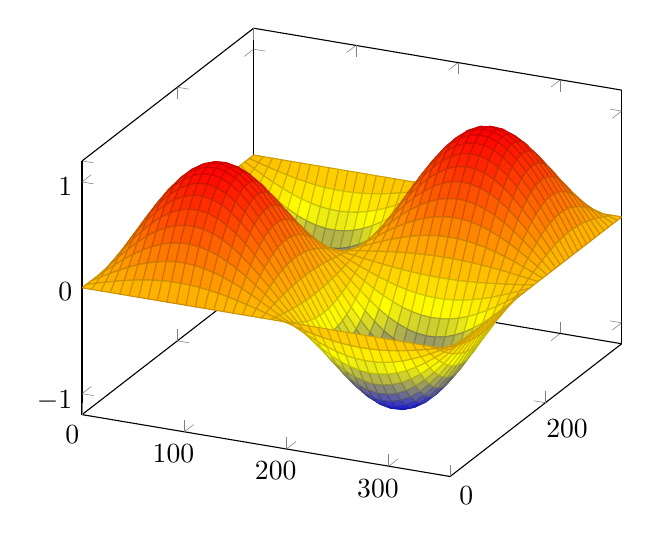
\begin{tikzpicture}
\begin{axis}
\addplot3[
surf,
domain=0:360,
samples=40,
] {sin(x)*sin(y)};
\end{axis}
\end{tikzpicture}
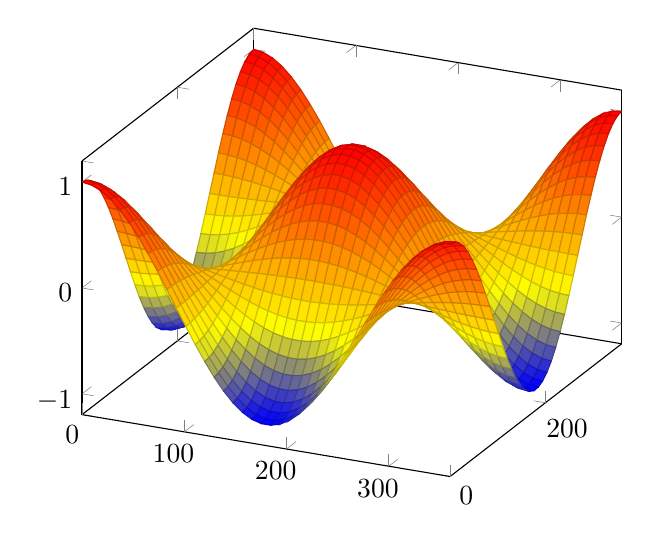
\begin{tikzpicture}
\begin{axis}
\addplot3[
surf,
domain=0:360,
samples=40,
] {cos(x)*cos(y)};
\end{axis}
\end{tikzpicture}

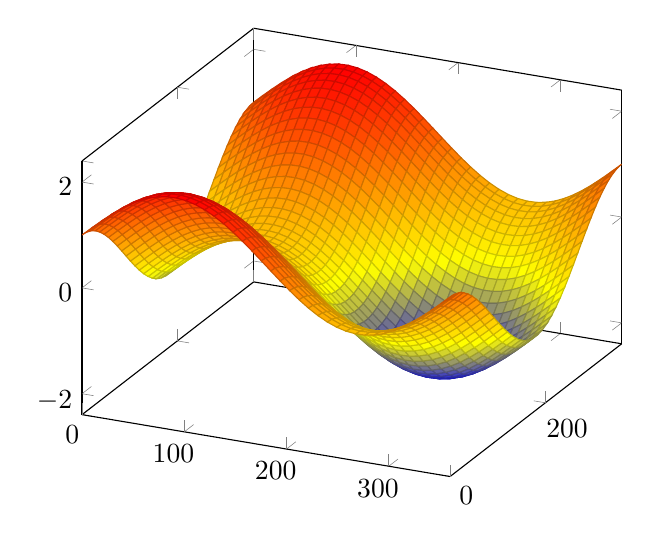
\begin{tikzpicture}
\begin{axis}
\addplot3[
surf,
domain=0:360,
samples=40,
] {sin(x)+cos(y)};
\end{axis}
\end{tikzpicture}
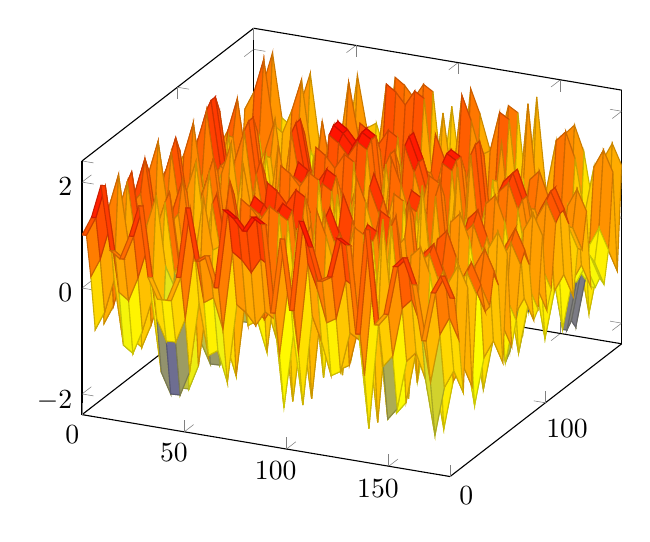
\begin{tikzpicture}
\begin{axis}
\addplot3[
surf,
domain=0:180,
samples=40,
] {sin(x*x)+cos(y*y)};
\end{axis}
\end{tikzpicture}

\begin{tikzpicture}
\begin{axis}
\addplot gnuplot [
id=sin,
] {sin(x)};
\end{axis}
\end{tikzpicture}


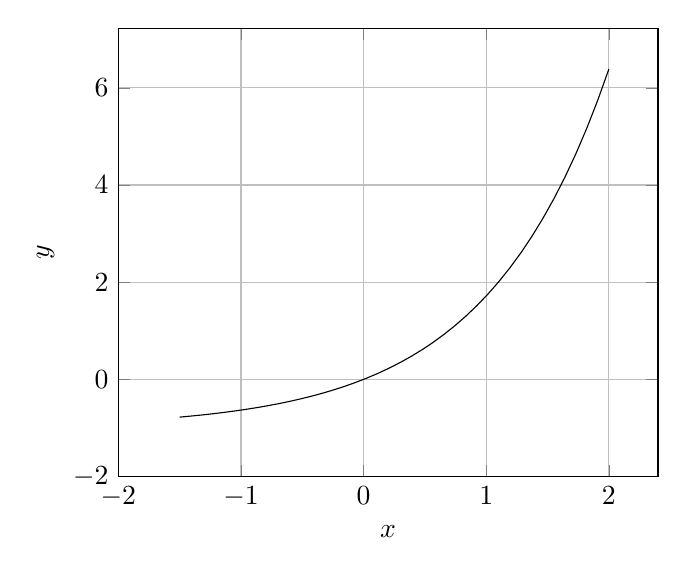
\begin{tikzpicture}
\begin{axis}[
xmin=-2,
ymin=-2,
xlabel= $x$,
ylabel= $y$,
grid=major,
]
\addplot[
domain=-1.5:2,
samples=40,
] {e^x-1};
\end{axis}
\end{tikzpicture}

\begin{tikzpicture}
\begin{axis}[
axis line=center,
xmin=-5.5,
ymin=-4,
xlabel= $x$,x label style={right},
ylabel= $y$,y label style= {above},
grid=major,
]
\addplot[
domain=-5.5:3,
samples=100,
] {1+x+x^2/2+x^3/6+x^4/24};
\end{axis}
\end{tikzpicture}


\begin{tikzpicture}
\datavisualization [school book axes, visualize as smooth line]
data [format=function] {
var x : interval [-1.3:1.3];
func y = \value x*\value x*\value x;
};
\end{tikzpicture}


\section{Symbols, Shortcuts and Semantic Aliasing}

Although Journals recommend not to alias LaTeX commands the harsh reality is that each topic and paper has different needs for notations and things can get messy.

Consider papers written for computations of floating algorithms. We might find in preambles definitions like, 
{\parskip0pt\large
\begin{verbatim}
%% Floating-point machine operations.
\newcommand{\mop}{\boxcircle}
\newcommand{\madd}{\boxplus}
\newcommand{\msub}{\boxminus}
\newcommand{\mmul}{\boxdot}
\newcommand{\mdiv}{\boxdiag}
\end{verbatim}
}
\newcommand{\mop}{\boxcircle}
\newcommand{\madd}{\boxplus}
\newcommand{\msub}{\boxminus}
\newcommand{\mmul}{\boxdot}
\newcommand{\mdiv}{\boxdiag}

I consider aliasing of non-semantic commands to semantic commands, such as the machine operation |\mop| from |\boxcircle| as good practice. 

\begin{texexample}{Example with macro aliasing}{ex;aliasing}
\begin{Definition} \summary{(Absorption.)}
Let $x, y, z \in \Fset$ with $y, z \in \Rset$,
let $\mathord{\mop}$ be any IEEE~754 floating-point operator,
and let $x = y \mop z$.
Then $y \mop z$ gives rise to \emph{absorption} if
\begin{itemize}
\item
$\mathord{\mop} = \mathord{\madd}$
and either $x = y$ and $z \neq 0$, or $x = z$ and $y \neq 0$;
\item
$\mathord{\mop} = \mathord{\msub}$
and either $x = y$ and $z \neq 0$, or $x = -z$ and $y \neq 0$;
\item
$\mathord{\mop} = \mathord{\mmul}$
and either $x = \pm y$ and $z \neq \pm 1$, or $x = \pm z$ and $y \neq \pm 1$;
\item
$\mathord{\mop} = \mathord{\mdiv}$,
$x = \pm y$ and $z \neq \pm 1$.
\end{itemize}
\end{Definition}
\end{texexample}


The most obvious shortcuts should be for calligraphic or fraktur math alphabets.


\begin{texexample}{Calligraphic Alphabet}{ex:callalphabet}
\providecommand*{\cA}{\ensuremath{\mathcal{A}}}
\providecommand*{\cB}{\ensuremath{\mathcal{B}}}
\providecommand*{\cC}{\ensuremath{\mathcal{C}}}
\providecommand*{\cD}{\ensuremath{\mathcal{D}}}
\providecommand*{\cE}{\ensuremath{\mathcal{E}}}
\providecommand*{\cF}{\ensuremath{\mathcal{F}}}
\providecommand*{\cG}{\ensuremath{\mathcal{G}}}
\providecommand*{\cH}{\ensuremath{\mathcal{H}}}
\providecommand*{\cI}{\ensuremath{\mathcal{I}}}
\providecommand*{\cJ}{\ensuremath{\mathcal{J}}}
\providecommand*{\cK}{\ensuremath{\mathcal{K}}}
\providecommand*{\cL}{\ensuremath{\mathcal{L}}}
\providecommand*{\cM}{\ensuremath{\mathcal{M}}}
\providecommand*{\cN}{\ensuremath{\mathcal{N}}}
\providecommand*{\cO}{\ensuremath{\mathcal{O}}}
\providecommand*{\cP}{\ensuremath{\mathcal{P}}}
\providecommand*{\cQ}{\ensuremath{\mathcal{Q}}}
\providecommand*{\cR}{\ensuremath{\mathcal{R}}}
\providecommand*{\cS}{\ensuremath{\mathcal{S}}}
\providecommand*{\cT}{\ensuremath{\mathcal{T}}}
\providecommand*{\cU}{\ensuremath{\mathcal{U}}}
\providecommand*{\cV}{\ensuremath{\mathcal{V}}}
\providecommand*{\cW}{\ensuremath{\mathcal{W}}}
\providecommand*{\cX}{\ensuremath{\mathcal{X}}}
\providecommand*{\cY}{\ensuremath{\mathcal{Y}}}
\providecommand*{\cZ}{\ensuremath{\mathcal{Z}}}
\begin{luacode}
local alphabet = {"A","B","C","D","E","F","G","H","I","J","K","L",
                  "M","N","O","P","Q","R","S","T","U",
                  "V","W","X","Y","Z"}
for k,v in pairs(alphabet) do
	tex.print("\\c"..v..", ")
end
\end{luacode}
\end{texexample}


\section{Calculus}



\subsection*{Differentiation}
Leibnitz invented the transmutation theorem for finding the area under a curve. Finding areas beneath curves
was 


\subsection*{Integration}

\subsection*{Limits}

\marginpar{\includegraphics[width=3cm]{bolzano}
{\scriptsize\RaggedLeft Bolzano begins his work by explaining what he means by theory of science, and the relation between our knowledge, truths and sciences. Human knowledge, he states, is made of all truths (or true propositions) that men know or have known. This is, however, only a very small fraction of all the truths that exist, although still too much for one human being to comprehend. Therefore, our knowledge is divided into more accessible parts. Such a collection of truths is what Bolzano calls a science (Wissenschaft). It is important to note that not all true propositions of a science have to be known to men; hence, this is how we can make discoveries in a science.}}

\textbf{Bolzano} Although implicit in the development of calculus of the 17th and 18th centuries, the modern idea of the limit of a function goes back to Bolzano who, in 1817, introduced the basics of the epsilon-delta technique to define continuous functions. However, his work was not known during his lifetime.\footcite{coolidge} The first publication in English had to wait for almost 150 years and it was published by Coolidge in 1949 in his popular work \emph{The Mathematetics of Great Amateurs.} Grattan-Guiness\footcite{grattan-guiness} falls short though of accusing Cauchy of plagiarizing the work of Bolzano and other contemporaries.


\textbf{Cauchy} discussed variable quantities, infinitesimals, and limits and defined continuity of {$\displaystyle y=f(x)$} $y=f(x)$ by saying that an infinitesimal change in $x$ necessarily produces an infinitesimal change in $y$ in his 1821 book \emph{Cours d'analyse}, while (Grabiner 1983) claims that he only gave a verbal definition. 

\textbf{Weierstrass} first introduced the epsilon-delta definition of limit in the form it is usually written today. He also introduced the notations $\lim$ and $\lim x\rightarrow x_0$. The notation which has been used widely at the time in Europe was
$\operatorname{Lim}_{x=a}$, to express the \enquote{the limit as $x$ approaches $a$.} It is found in papers of Weierstrass, who in 1841 wrote $\lim$ and in 1854 \enquote{$\underset{n=\infty}{\operatorname{Lim.}}\:p_n = \infty $}

In later publications we find $\operatorname{Lim}$ without the point, but still capitalized. I particularly like the way the equations were grouped and the limit indicated by cases and shown in fig.~\ref{weis}.

\begin{figure}[htbp]
\centering
\includegraphics[width=0.8\textwidth]{weistrass}
\caption{Extract from Weierstrass publication.}
\label{weis}

\end{figure}

To create a new operator symbol we can use \cs{operatorname}. The command will take care of spacing, whereas if we use only
|\mathrm| it will not. If we were to use it frequently we could also define a macro using \cs{DeclareMathOperator} from amsmath. 

\begin{texexample}{operatorname}{ex:onames}

$$\operatorname{Lim.}p_n$$

$$\operatorname{Lim}.p_n$$

$$\mathrm{Lim.}p_n$$ 
\end{texexample}

By the early 1900's the notation started approaching more to what is commonly used in today's publications.

\textbf{Hardy} The modern notation of placing the arrow below the limit symbol is due to Hardy in his book \emph{A Course of Pure Mathematics} in 1908, however in the preface to the book he credits Leathem and Bromwich\footcite{bromwich}.\footnote{Hardy wrote ... there are two respects in which I have diverted ...} 


\begin{gather}
\begin{aligned}
f(a) &= f\left[\lim_{k\rightarrow\infty} x_k \right]=\lim_{k} f(x_k)\le 0 & \text{ and }\\
f(a) &= f\left[\lim_{k\rightarrow\infty} X_k \right]=\lim_{k} f(X_k)\ge 0. & \\  
\end{aligned}
\end{gather}

In Cauchy's words, these inequalities established that ``the quantity
$f(a)$ \ldots cannot differ from zero.'' He had thus proved the existence of a
number a between $x$ and $X$ for which $f(a) = O$. The general version of the
intermediate value theorem, namely that a continuous function takes all
values between $f(x_0)$ and $f(X)$, follows as an easy corollary.
This was a remarkable achievement. Cauchy had, for the most part,
succeeded in demonstrating a "self-evident" principle by analytic methods.


Apart from open intervals, limits can be defined for functions on arbitrary subsets of R, as follows.  Let $f$ be a real-valued function defined on a subset $S$ of the real line.  Let $p$ be a limit point of ''S'' that is, ''p'' is the limit of some sequence of elements of ''S'' distinct from p.  The limit of ''f'', as ''x'' approaches ''p'' from values in ''S'', is ''L'' if, for every {{nowrap|''ε'' > ''0''}}, there exists a δ > ''0'' such that {{nowrap|0 < {{abs|''x'' − ''p''}} < ''δ''}} and {{nowrap|''x'' ∈ ''S''}} implies {{nowrap|{{abs|''f''(''x'') − ''L''}} < $\epsilon$.

This limit is often written

\[
L = \underset{x\in S}{\lim_{x\to p}} f(x).
\]

The condition that $f$ be defined on $S$ is that $S$ be a subset of the domain of $f$.  This generalization includes as special cases limits on an interval, as well as left-handed limits of real-valued functions (e.g., by taking ''S'' to be an open interval of the form $(-\infty,a)$, and right-handed limits (e.g., by taking ''S'' to be an open interval of the form $(a,\infty)$. It also extends the notion of one-sided limits to the included endpoints of (half-)closed intervals, so the Square root function $f(x)=\sqrt{x}$ can have limit 0 as $x$ approaches 0 from above.




\section*{Fraktur letters}

Individual Fraktur letters are sometimes used in mathematics, which often denotes associated or parallel concepts by the same letter in different fonts. For example, a Lie group is often denoted by ''G'', while its associated Lie algebra is $\mathfrak{g}$. 
A ring ideal might be denoted by $\mathfrak{a}$ (or $\mathfrak{p}$ if a prime ideal) while an element is $a \in \mathfrak{a}$. The Fraktur $\mathfrak c$ is also sometimes used to denote the cardinality of the continuum, that is, the cardinality of the real line. In model theory, $\mathfrak{A}$ is used to denote an arbitrary model, with ''A'' as its universe. Fraktur is also used in other ways at the discretion of the author.


\begin{luacode}
local alphabet = {"A","B","C","D","E","F","G","H","I","J","K","L",
                  "M","N","O","P","Q","R","S","T","U","V","W","X","Y","Z"}
for k,v in pairs(alphabet) do
	tex.print("\\mathfrak{"..v.."}, ")
end
\end{luacode}

Special symbols such as dingbats loaded using the \pkg{pifont} package need to be enclosed within an \docAuxCommand{mbox} in order to be able to display the glyph properly.
\bigskip

\begin{texexample}{Using special dingbat symbols}{}
\label{e14}
 We start by showing that the function $f(x)=x^2$ is
continuous over the set $X_2$\label{p:X2} defined as the interval
$[0,1]$ where numerals $\frac{i}{\mbox{\ding{172}}}, 0 \le i \le
\mbox{\ding{172}},$ are used to express its points in units $\mu$.
First of all, note that the set $X_2$ is continuous in   $\mu$
because its points are equidistant with the distance
$d=\mbox{\ding{172}}^{-1}$. Since this function is strictly
increasing,  to show its continuity it is sufficient to check the
difference $f(x)-f(x^{-})$ at the point $x=1$. In this case,
$x^{-}=1-\mbox{\ding{172}}^{-1}$ and we have
\[
 f(1)-f(1-\mbox{\ding{172}}^{-1})=
 1-(1-\mbox{\ding{172}}^{-1})^2 =
 2\mbox{\ding{172}}^{-1}(-1)\mbox{\ding{172}}^{-2}.
\]
This number is infinitesimal, thus $f(x)=x^2$ is continuous over
the set $X_2$. \hfill $\Box$
\end{texexample}

\cs{Box}
Notice the use of the \docAuxCommand{Box} command to draw a square for  end of proof symbol. This is from the amsmath package. The box is placed at the end of the line using |\hfill $\Box$|.

%
%\begin{Rule}
%Alias common symbols to semantic macro names that follow their mathematical definitions.
%\end{Rule}
%
%\begin{Rule}
%Create shorcut commands with moderation for alphabets and algebras and alias if necessary. Good practice, sets etc.
%\end{Rule}



\section{Partial derivatives}

Partial derivatives can be typeset using the \latex{} command \cs{partial}

\begin{texexample}{Partial Derivatives}{ex:partial}
\[
dS = \frac{\partial S}{\partial x}\, dx
   + \frac{\partial S}{\partial y}\, dy
   = \left(y - \frac{2V}{x^2}\right) dx
   + \left(x - \frac{2V}{y^2}\right) dy.
\]
\meaning\partial
\end{texexample}


This is using a certain style. For other styles it maybe more difficult.

\section*{Binomial Coefficients}

To typeset binomial coefficients or similar structures, use the command
\cs{binom} from \pkg{amsmath}\index{amsmath>binom}

\begin{texexample}{Binomial}{ex:binomial0}
\[
\begin{align}
(x+y)^3 & = x^3 + 3x^2y + 3xy^2 + y^3, \\[8pt]
(x+y)^4 & = x^4 + 4x^3y + 6x^2y^2 + 4xy^3 + y^4, \\[8pt]
(x+y)^5 & = x^5 + 5x^4y + 10x^3y^2 + 10x^2y^3 + 5xy^4 + y^5, \\[8pt]
(x+y)^6 & = x^6 + 6x^5y + 15x^4y^2 + 20x^3y^3 + 15x^2y^4 + 6xy^5 + y^6, \\[8pt]
(x+y)^7 & = x^7 + 7x^6y + 21x^5y^2 + 35x^4y^3 + 35x^3y^4 + 21x^2y^5 + 7xy^6 + y^7.
\end{align}
\]
\end{texexample}


Pascal's rule can be typeset as:


\begin{texexample}{Binomial Distribution}{ex:binomial}
\[
\binom{n}{k} =\binom{n-1}{k}
+ \binom{n-1}{k-1}
\]
\end{texexample}



\section[Symbols and Abbreviations]{Symbols and Abreviations}
\label{math:abbreviations}

\label{abbr}\label{symbols}%

\begin{texexample}{Creating symbols}{ex:parallelogram}
\newlength{\dentwidth}\setlength{\dentwidth}{\textwidth}
\addtolength{\dentwidth}{-\parindent}

\makeatletter
\gdef\@parallelogram#1{%
  \textnormal{\setbox\z@\hbox{#1/}\dimen@\wd\z@
   \@tempdima 2.45\dimen@
   \vbox{\offinterlineskip
      \hbox{\kern.8\dimen@\vrule\@width\@tempdima\@height.4\p@}%
      \kern-.0\p@
      \hbox to\@tempdima{#1/\hfil\rlap/}%
      \kern-.5\p@
      \hbox{\kern.1\dimen@\vrule\@width\@tempdima\@height.4\p@}}}}
      
 \gdef\Par{%
   \mathchoice
      {\@parallelogram\scriptsize}%
      {\@parallelogram\scriptsize}%
      {\@parallelogram\tiny}%
      {\@parallelogram\tiny}}

            



\begin{tabular*}{\dentwidth}{rl@{\extracolsep{\fill}}l@{\extracolsep{0pt}}@{\dots}l}

$>$ & is (or are) greater than. & Def. & definition. \\
$<$ & is (or are) less than. & Ax. & axiom. \\
$\Bumpeq$ & is (or are) equivalent to. & Hyp. & hypothesis. \\
$\therefore$ & therefore. & Cor. & corollary. \\
$\perp$ & perpendicular. & Scho. & scholium. \\
$\perp_s$ & perpendiculars. & Ex. & exercise. \\
$\parallel$ & parallel.\qquad $\parallel_s$ parallels. & Adj. & adjacent. \\
$\angle$ & angle.\qquad $\angle_s$ angles. & Iden. & identical. \\
$\triangle$ & triangle.\qquad $\triangle_s$ triangles. & Const. & construction. \\
$\Par$ & parallelogram. & Sup. & supplementary. \\
$\Par_s$ & parallelograms. & Ext. & exterior. \\
$\odot$ & circle.\qquad $\odot_s$ circles. & Int. & interior. \\
rt. & right.\qquad  st.\ straight. & Alt. & alternate. \\
\end{tabular*}


\hbox{\qed\ stands for quod erat demonstrandum, \emph{which was to be proved}.\hss}

\newcommand{\qef}{\textsc{q.e.f.}}
\qef\ stands for quod erat faciendum, \emph{which was to be done.}

The signs $+$, $-$, $\times$, $\div$, $=$, have the same meaning as in Algebra.

\makeatother   
\end{texexample}
   
\section{Afixing symbols to other symbols}

\latex provides \docAuxCommand{stackrel} for placing a superscript above a binary relation. In the \pkg{amsmath} package there are somewhat more general commands \docAuxCommand{overset} and \docAuxCommand{underset}, that can be used to place one symbol above or below another symbol, whether is a relation or something else. Oberdiek's package \pkg{stackrel}\footcite{stackrel} extends the syntax by adding an optional argument for the subscript position. It follows the syntax of extensible arrows of the packages |amsmath| and |mathtools|.

\begin{docCommand}{stackrel}{\oarg{subscript}\marg{superscript}{\marg{rel}}}
  Typeset a subscript or superscript above a symbol.
\end{docCommand}

\ifSTACKREL
\begin{texexample}{Example of stackrel and stackbin}{ex:stackrel}
\[
 A \stackbin[\text{and}]{}{+} B \stackrel[x]{!}{=} C
\] 
\end{texexample}
\else
\begin{texcode}{Example of \cs{stackrel} and \cs{stackbin}}{ex:stackrel}
  Example cannot be shown as the package stackrel is not loaded.
\end{texcode}
\fi


\chapter{Matrices and Mathematical Environments}
\label{matrices}

\section{Matrices}

Matrices have a long history of application in solving linear equations but they were known as arrays until the 1800s. The Chinese text The Nine Chapters on the Mathematical Art written in 10th–2nd century BCE is the first example of the use of array methods to solve simultaneous equations,[102] including the concept of determinants. In 1545 Italian mathematician Gerolamo Cardano brought the method to Europe when he published Ars Magna.[103] The Japanese mathematician Seki used the same array methods to solve simultaneous equations in 1683.[104] 


The Dutch statesman and mathematician Johan (Jan) de Witt represented transformations resembling arrays in his 1659 book Elements of Curves (1659). He is also perhaps the second Mathematician to be lynched\footnote{Hypatia, was torn to bits by a lynching Christian mob in the streets of Alexandria in \textsc{AD} 415.} by a mob and had parts of their bodies eaten! [\ldots]The brothers were shot and then left to the mob. Their naked, mutilated bodies were strung up on the nearby public gibbet, while the Orangist mob partook of their roasted livers in a cannibalistic frenzy. Throughout it all, a remarkable discipline was maintained by the mob, according to contemporary observers, making one doubt the spontaneity of the event.\footcite{israel1995} \textit{Elementa Curvarum Linearum} has been described as the first textbook in analytic geometry.\footnote{The savage murder of a man that history has judged a highly competent leader is regarded by the Dutch as one of the most shameful episodes in their history.}


Between 1700 and 1710 Gottfried Wilhelm Leibniz publicized the use of arrays for recording information or solutions and experimented with over 50 different systems of arrays.[103] Cramer presented his rule in 1750.

The term "matrix" (Latin for "womb", derived from mater—mother[106]) was coined by James Joseph Sylvester in 1850,[107] who understood a matrix as an object giving rise to a number of determinants today called minors, that is to say, determinants of smaller matrices that derive from the original one by removing columns and rows. In an 1851 paper, Sylvester explains:

\begin{quote}
I have in previous papers defined a \enquote{Matrix} as a rectangular array of terms, out of which different systems of determinants may be engendered as from the womb of a common parent.[108]
\end{quote}

Arthur Cayley published a treatise on geometric transformations using matrices that were not rotated versions of the coefficients being investigated as had previously been done. Instead he defined operations such as addition, subtraction, multiplication, and division as transformations of those matrices and showed the associative and distributive properties held true. Cayley investigated and demonstrated the non-commutative property of matrix multiplication as well as the commutative property of matrix addition.[103] Early matrix theory had limited the use of arrays almost exclusively to determinants and Arthur Cayley's abstract matrix operations were revolutionary. He was instrumental in proposing a matrix concept independent of equation systems. In 1858 Cayley published his A memoir on the theory of matrices[109][110] in which he proposed and demonstrated the Cayley–Hamilton theorem.[103] Cayley introduced a particular notation for fencing the array as shown in fig~\ref{fig:cayley}, which used () for the first row and $\vert$ for subsequent rows.

\begin{figure}[htbp]
\centering
\includegraphics[width=0.6\textwidth]{cayley-notation}

\caption{Extract from Caley's paper \textit{A memoir on the theory of matrices.}}
\label{fig:cayley}

\end{figure}

An English mathematician named Cullis was the first to use modern bracket notation for matrices in 1913 and he simultaneously demonstrated the first significant use of the notation $A = [a_{i,j}]$ to represent a matrix where $a_{i,j}$ refers to the i$^$th row and the $j$th column.

Cayley's introductory paper in matrix theory was written in French and published in a German periodical. In this paper, matrices are introduced to simplify the notation which arises in simultaneous linear equations.  

\begin{gather}
\begin{aligned}
\xi  &= \alpha x + \beta y + \gamma z + \dots\\
\eta  &= \alpha' x + \beta' y + \gamma' z + \dots\\
\zeta &= \alpha'' x + \beta'' y + \gamma'' z + \dots
\end{aligned}
\end{gather}

The set of equations is written as:

\begin{gather}
(\xi, \eta, \zeta,\dots ) = (\alpha,\beta,\gamma,\dots)(x,y,z,\dots)
\end{gather}

The same article also introduces, although quite sketchily, the ideas of inverse matrix and of matrix multiplication, or \enquote{compounding} as Cayley called it. The above basic properties are expanded in a second expository article\footcite{fieldman1962} which
also lists many additional properties of matrices. In this important paper, Cayley works mostly with square matrices with
nine elements. He represents the zero matrix,\footcite[This is an interesting development]{fieldman1962}

\[
\begin{vmatrix}
0,0,0\\
0,0,0\\
0,0,0
\end{vmatrix}
\]
by \enquote{0} and the \enquote{matrix unity,}

\[
\begin{vmatrix}
1,0,0\\
0,1,0\\
0,0,1
\end{vmatrix}
\]
by \enquote{1}

Caley then introduces the algebra of matrices by defining the addition of two matrices by

\begin{gather}
(\begin{cayleymatrix}{3}
a&b&c\\
a' &b' & c'\\
a''&b'' & c''\\
a''' & b''' & c'''\\
\end{cayleymatrix}) +
(\begin{cayleymatrix}{3}
\alpha & \beta & \gamma\\
\alpha & \beta & \gamma\\
\alpha & \beta & \gamma\\
\end{cayleymatrix})\:\: = \:\:
(\begin{cayleymatrix}{3}
a+a  &b+b  &c+\gamma\\
a''+\alpha' & b'' + \beta'' & c'' +\gamma'' \\
a'''+\alpha''' & b''' + \beta''' & c''' +\gamma''' \\
\end{cayleymatrix})
\end{gather}
Caley stated but without proof, that matrices are commutative and associative under addition. Two types
of multiplication are exhibited. The first type is designated as \enquote{scalar multiplication,} that is

\[
m(\begin{cayleymatrix}{3}
a & b & c\\
a' & b' & c'\\
a'' & b'' & c''
\end{cayleymatrix}) 
= 
(\begin{cayleymatrix}{3}
ma & mb & mc\\
ma' & mb' & mc'\\
ma'' & mb'' & mc''
\end{cayleymatrix})
\]

The notation used for the matrix (\begin{cayleymatrix}{3}
a&b\\
c&d\\
e&f
\end{cayleymatrix}) is defined later on. It is a special environment.

The second type of multiplication is called \enquote{compounding,} according to the following scheme:

\begin{multline}
(\begin{cayleymatrix}{3}
a  &b &c\\
a' &b' &c'\\
a'' &b'' &c''
\end{cayleymatrix}\between \begin{cayleymatrix}{3}
\alpha & \beta & \gamma\\
\alpha'' & \beta'' & \gamma''\\
\alpha'' & \beta'' & \gamma''\\
\end{cayleymatrix})
\\=
 (\begin{cayleymatrix}{3} \bigl(a,b,c\between a, a',a''\bigr) & (a,b,c\between (\beta, \beta', \beta'') & (a,b,c\between \gamma, \gamma', \gamma'')\\
(a &b &c\\
(a &b &c
\end{cayleymatrix})\label{caleyprod}
\end{multline}

The product equation is complex to type, but very clear to understand its definition.\footnote{Uses multline environment.}


Later developments are described by Feldmann\footcite[This is the second paper that appeared in the \textit{The Mathematics Teacher relating to matrices.}][]{feldmann1963}. 

In the 1930s books on matrices written in English started to appear. The two leading ones were C.C. MacDuffee \textit{Theory of Matrices,} Springer (1933) and J. H. M. Wedderburn \textit{Lectures on Matrices}\footnote{The book was published by the American Mathematical Society and bears reseblance to a publication printed using TeX.} (1934). They both wrote matrices with double vertical lines as in

\[
\begin{Vmatrix}
a_{11} & a_{12} & \dots & a_{1n}\\
a_{11} & a_{12} & \dots & a_{1n}\\
\vdots & \vdots & \vdots & \vdots\\
a_{n1} & a_{n2} & \dots &a_{nn}
\end{Vmatrix}
\]
The use of double vertical lines was easy to typeset as well as to handwrite. It could also relate to the single vertical lines which are used to denote determinants.




%%%%%%%%%%%%%%%%%%%%%%%%%%%%%%%%%%%%%%%%%%%%%
%%%%%%%%  TYPOGRAPHY %%%%%%%%%%%%%%%%%%%%%%%%
\section{Typography of Matrices}

Matrices are mostly typed the way tabular environements are types, i.e., you need to use the tabulator sign ``\&''.
Mathematical environments are provided both by \latexe as well as amsmath. The latter are to be preferred.

\begin{docEnvironment}{array}{\marg{specifier}}
\end{docEnvironment}

The |array| environment is a \latex2e provided environment and is identical to tabular, but works automatically with mathematics. It has to be enclosed in a mathematical environment.


\begin{texexample}{Matrices}{ex:matrices}
\[
\mathbf{X} = \left(
\begin{array}{ccc}
x_1 & x_2 & \ldots \\
x_3 & x_4 & \ldots \\
\vdots & \vdots & \ddots
\end{array} \right)
\]
\end{texexample}

\section{AMS Math matrices}

The \pkg{amsmath} package provides environments that go beyond the basic \docAuxEnvironment{array} of \latex2e. The \docAuxEnvironment{pmatrix}, \docAuxEnvironment{Bmatrix}, \docAuxEnvironment{vmatrix} and \docAuxEnvironment{Vmatrix}. 
There is also a \docAuxEnvironment{smallmatrix} that is more suitable for inline text display. 

\begin{texexample}{Using \textbackslash smallmatrix}{ex:smallmatrix}
This is a small matrix $\bigl(\begin{smallmatrix}
a&b\\
c&d\\
\end{smallmatrix}\bigr)$ environment. \lorem
\end{texexample}


\begin{docEnvironment}{bmatrix}{}
The example \ref{ex:bmatrix} illustrates the typesetting of a bracketted matrix hence \ul{b}matrix. If you want the matrix equation to be numbered enclose it withn an |equation| or |gather| environment. In this documentation we have let the |equation| environment to |gather| hence it will make no difference which ever is used. (amsmath)
\end{docEnvironment}

\begin{texexample}{Bmatrix}{ex:bmatrix}
\begin{equation}
\begin{matrix}
1 & 2 \\
3 & 4
\end{matrix} \qquad
\begin{bmatrix}
p_{11} & p_{12} & \ldots & p_{1n} \\
p_{21} & p_{22} & \ldots & p_{2n} \\
\vdots & \vdots & \ddots & \vdots \\
p_{m1} & p_{m2} & \ldots & p_{mn}
\end{bmatrix}
\end{equation}
\end{texexample}

The \refEnv{bmatrix} is from the amsmath package, see also \vref{bmatrix} and \nameref{bmatrix} and \pageref{bmatrix}. 


One issue to be aware is that the \refEnv{bmatrix} does not allow more than 10 tab stops. If you need to use more, you will have to \docCounter{MaxMatrixCols} to a higher number. The |phd| package sets this automatically at 20, so you will not have to worry about it.

\begin{teX}
\setcounter{MaxMatrixCols}{20}
\end{teX}

\begin{texexample}{Large Matrices}{ex:largematrices}
\[
\begin{bmatrix}
1 & 0 & 0 & -1 & 0  & 0  & 1 & -1 & 1  & -1 & 0 \\
0 & 1 & 0 & 0  & -1 & 0  & 1 & -1 & 0  & 1  & -1 \\
0 & 0 & 1 & 0  & 0  & -1 & 1 & -1 & -1 & 0  & 1 
\end{bmatrix}
\]
\end{texexample}



\section{vmatrix}

\begin{texexample}{vmatrix}{ex:vmatrix}

\begin{gather}
\begin{vmatrix}
aa' + bb' + cc' & ea' + fb' + gc' \\
ae' + bf' + cg' & ee' + ff' + gg'
\end{vmatrix}
{} = \begin{vmatrix}
a & b \\
e & f
\end{vmatrix}  \begin{vmatrix}
a' & b' \\
e' & f'
\end{vmatrix} + \begin{vmatrix}
a & c \\
e & g
\end{vmatrix}  \begin{vmatrix}
a' & c' \\
e' & g'
\end{vmatrix}.
\end{gather}
\end{texexample}





\section{Single equations that are too long}

In many cases equations need to be written over two or more lines. The \pkgname{amsmath} package, provides environments that are suitable for this:


\begin{texexample}{The multiline amsmath environment}{ex:multiline}
\begin{multline}
   a + b + c + d + e + f+ g + h + i  + k + l + m + n + o + p\\
              = j + k + l + m + n +\cos^{2}-1
\end{multline}
\end{texexample}



\section{array environment}

This is simply the same as the |eqnarray| environment only with the possibility of
variable rows and columns and the fact, that the whole formula has only one
equation number and that the array environment can only be part of another math
environment, like the equation environment or the displaymath environment. With
@{} before the first and after the last column the additional space |\arraycolsep| is
not used, which maybe important when using left aligned equations.

\begin{texexample}{array environment}{ex:array2}
\begin{eqnarray}
  a & = & b + c \\
    & = & d + e + f + g + h + i
               + j + k + l \nonumber \\
    &   & +\: m + n + o \\
    & = & p + q + r + s
\end{eqnarray}
\end{texexample}

The equations
to be aligned are entered with each one terminated by \cs{cr}. In each equation there should be
one alignment symbol \& to indicate where the alignment should take place. This is usually
done at the equal signs, although it is not necessary to do so. For example


\begin{texexample}{The array environment}{ex:array}
Thus to change $\frac34$ to a decimal divide $4$ into $3$
and we get $.75$ as a result, thus:
\[
\begin{array}{r@{}r@{}}
4 \; & \vline \; 3.00 \\\cline{2-2}
     &            .75
\end{array}
\]

To find the square root of a four-figure number
such as our example calls for, work it out in the
following manner:
\[
\arraycolsep=0em
\begin{array}{cccccccccccc}
\multicolumn{3}{c}{\text{2d pair}} &\qquad&\qquad&
\multicolumn{3}{c}{\text{1st pair}}&\qquad&\qquad&
\multicolumn{2}{c}{\text{square root}}\\
 & \overbrace{\quad}&\ZZZ&&&\ZZZ&\overbrace{\quad}&\ZZZ\\
 & 42 &&&&& 25 &&&&\vline\;65&(answer)\\\cline{11-11}
 & 36 &&&&& \\\cline{2-2}
\multirow{2}{*}{125\:} & \vline\hfill \Zi6 \hfill&&&&& 25\\
 & \vline\hfill \Zi6 \hfill&&&&& 25\\\cline{2-7}
\end{array}
\]
\end{texexample}


\subsection{Array environment in game theory}

This example \ref{ex:gamearray} is from \footnote{From determinacy to Nash equilibrium,St\'ephane Le Roux, TU Darmstadt }

\begin{texexample}{array environment in game theory}{ex:gamearray}
The game $\langle\{a,b,c\},\{1,2,3,4\}^3,\{0,1,2,3,4\},v,(<_d)_{d\in\{a,b,c\}}
\rangle$ is represented below, where player $a$ chooses the row, $b$ the column, and $c$ the array. 
\[\begin{array}{c@{\hspace{1cm}}c@{\hspace{1cm}}c@{\hspace{1cm}}c}
\begin{array}{|c|c|c|c|}
\hline 1 & 1 & 1 & 1\\
\hline 1 & 1 & 1 & 1\\
\hline 1 & 1 & 1 & 1\\
\hline 4 & 1 & 1 & 1\\
\hline
\end{array}
&
\begin{array}{|c|c|c|c|}
\hline 1 & 2 & 1 & 1\\
\hline 2 & 2 & 2 & 2\\
\hline 1 & 2 & 1 & 1\\
\hline 4 & 2 & 1 & 1\\
\hline
\end{array}
&
\begin{array}{|c|c|c|c|}
\hline 1 & 1 & 3 & 1\\
\hline 1 & 1 & 3 & 1\\
\hline 3 & 3 & 3 & 3\\
\hline 4 & 1 & 3 & 1\\
\hline
\end{array}
&
\begin{array}{|c|c|c|c|}
\hline 2 & 4 & 4 & 4\\
\hline 4 & 3 & 4 & 4\\
\hline 4 & 4 & 4 & 4\\
\hline 0 & 0 & 0 & 0\\
\hline
\end{array}
\end{array}
\]
Let us show that the game $\langle\{a,b,c\},\{1,\dots,n\}^3,\{0,\dots,n\},v,(<_d)_{d\in\{a,b,c\}}
\rangle$ witnesses the claim. First, the preferences are linear orders indeed. Second, let us show that there is no Nash equilibrium by case-splitting below. 
\end{texexample}



\section{The AMSmath Package}

\index{maths environment>align}
\index{maths environment>align}
\index{maths environments}{falign}
\index{maths environments}{xalignat}
\index{maths environments}{xxalignat}
\index{maths environments}{eqnarray}

The \pkg{amsmath} package offers five different align environments, |align|, |alignat|, |falign|, |xalignat| and |xxalignat|. 

In difference to the \refEnv{eqnarray} environment from standard \latex the ``three'' parts of one equation expr.-symbol-expr. are divided by only one ampersand in two parts. In general the ampersand should be before the symbol to get the right spacing, for example y \&= x. 

\subsection{The align environment}

The |align| environment is considered an improvement over \latex's |eqnarray| environment. It is very similar to a tabular
environment and is aligned at the |&|. 
It requires one |&| less and produces a tighter equation. Mathematicians 
are very particular in not using |eqnarray| and the package 
\pkgname{onlyamsomath} if used will warn if it finds that it has been used in the document. 
\index{eqnarray (environment)>spacing}
\index{eqnarray (environment)>alternatives}
\index{math environments>align}
\index{math environmenta>eqnarray}


\begin{texexample}{Comparison between |align| and |eqnarray|}{ex:eqnarraycomp}
% First example with eqnarray
\begin{eqnarray}
a & = & b + c \\
  & = & d + e + f + g + h + i
        + j + k + l \nonumber \\
  &   & +\: m + n + o \\
  & = & p + q + r + s
\end{eqnarray}

% Second example with align
\begin{align}
a & =  b + c \\
  & =  d + e + f + g + h + i
       + j + k + l \nonumber \\
  & +\: m + n + o \\
  & =  p + q + r + s
\end{align}
\end{texexample}


You can observe in Example~\ref{eqnarraycomp} the essential differences between the two, which we re-iterate, it requires one less |&| and produces a tighter display.

\begin{texexample}{The align environment}{ex:align}
\begin{align}
         y & = d\label{eq:IntoSection}\\
         y & = cx+d\\
    y_{12} & = bx^{2}+cx+d\\
     y(x)  & = ax^{3}+bx^{2}+cx+d
 \end{align}

%\begin{align*}
%\therefore (13 - x_1) + (13 - x_2) + \dotsb + (13 - x_p) + r &= 52\,,\\
%\therefore 13p - (x_1 + x_2 + \dotsb + x_p) + r              &= 52\,,\\
%\therefore x_1 + x_2 + \dotsb + x_p                          &= 13p - 52 + r\\
%                                                          &= 13 (p - 4) + r\,.
%\end{align*}

whence we conclude that $\gamma$ is a primitive root modulo $p$. But
\begin{align*}
\gamma^{p-1}-1 &=
     g^{p-1} - 1 + \frac{p-1}{1!}g^{p-2}xp +
        \frac{(p-1)(p-2)}{2!}g^{p-3}x^2p^2 + \ldots \\
  &= p\left(kp + \frac{p-1}{1!}g^{p-2}x +
        \frac{(p-1)(p-2)}{2!}g^{p-3}x^2p + \ldots\right).
\end{align*}
\end{texexample}

As you can observe from example\ref{ex:align}, each line is numbered if the unstarred version of the command is used. The |aligned| environment remedies this.
 


\subsection{The aligned environment}

The aligned environment allows more than one horizontal alignment but has only one equation number.

%\newcommand{\dotsbsmall}{\ldot\!\ldot\!\ldot}
%\newcommand{\ldot}{\mathbin{.}}			% dot with math spacing
%\newcommand{\nobf}[1]{\no \textbf{#1}}		% no with bold number
%
%\begin{texexample}{aligned environment example}{}
%\begin{equation}
%\begin{aligned}
%  &\:C_1x^{r_1}\,[\varphi_{r_1 0} \,+ \varphi_{r_1 1}\log x \,+ \dotsb + \varphi_{r_1 \alpha_1}(\log x)^{\alpha_1}]\\
%+ &\:C_2x^{r_2}\,[\varphi_{r_2 0} \,+ \varphi_{r_2 1}\log x \,+ \dotsb + \varphi_{r_2 \alpha_2}(\log x)^{\alpha_2}]\\
%+ &\multispan{1}{\:\dotfill}\\
%+ &\:C_nx^{r_n}[\varphi_{r_n 0} + \varphi_{r_n 1}\log x + \dotsb + \varphi_{r_n \alpha_n}(\log x)^{\alpha_n}],
%\end{aligned}
%\end{equation}
%
%\[
%\tag{98}
%\left\{\qquad
%\begin{aligned}
%T_1 &= T_2 = T_3 (=T)\\
%p_1 &= p_2 = p_3\\
%s_1-s_2 &= \frac{(u_1-u_2)+p_1(v_1-v_2)}{T}\\
%s_2-s_3 &= \frac{(u_2-u_3)+p_2(v_2-v_3)}{T}.
%\end{aligned}
%\right.
%\]
%\end{texexample}
 




\subsection{How to interrupt a display}

\begin{docCommand}{intertext}{}
 In many instances you will want to interrupt a display with some text. This can be accomplished using the control sequence |\intertext|.
 \end{docCommand}
 
 

\begin{texexample}{Using \cs{intertext}}{ex:intertext}
\begin{gather}
\begin{aligned}
U &= M u = M(c_v T + b)\\
S &= M(c_v  \log T + \frac{R}{m}  \log v + a),\\
\intertext{and } 
F &= M \left\{T(c_v - a - c_v \log T) - \frac{RT}{m} \log v + b \right\}.
\end{aligned}
\end{gather}
\end{texexample}

As the command \docAuxCommand{intertext} can only come after a |\\|  command we place it accordingly at {1}. Its function is to preserve the alignment after the text is typeset. This is a common requirement in many mathematical 
structures and the command can be used in all of amsmath aligning environments.







\subsection{The alignat environment}

\begin{docEnvironment}{alignat}{}
The alignat environment means \emph{align at} and can be used to align a set of equations vertically at more than one place. The star version of the environment omits the equation numbering.
\end{docEnvironment}


%\begin{texexample}{The alignat environment}{}
%\renewcommand{\dotsb}{\ldots}			% use lower dots after +-
%\renewcommand{\dotsbsmall}{\ldot\!\ldot\!\ldot}
%\renewcommand{\ldot}{\mathbin{.}}			% dot with math spacing
%\renewcommand{\nobf}[1]{\no \textbf{#1}}	
%
%\begin{alignat*}{5}
%  &p_{i+1}\dfrac{d^{m-i-1}y_1}{dx^{m-i-1}} &&+ \dotsbsmall +p_{m}y_1
%  && = -\Big(\dfrac{d^{m}y_1}{dx^{m}} &&+p_1\dfrac{d^{m-1}y_1}{dx^{m-1}}
%  &&+ \dotsbsmall +p_{i}\dfrac{d^{m-i}y_1}{dx^{m-i}}\Big), \\
%\multispan{10}{\makebox[36em]{\dotfill},}\\
% &p_{i+1}\dfrac{d^{m-i-1}y_{m-i}}{dx^{m-i-1}} &&+ \dotsbsmall +p_{m}y_{m-i}\!
% &&= -\Big(\dfrac{d^{m}y_{m-i}}{dx^{m}} &&+ p_1\dfrac{d^{m-1}y_{m-i}}{dx^{m-1}}
% &&+ \dotsbsmall +p_{i}\dfrac{d^{m-i}y_{m-i}}{dx^{m-i}}\Big).
%\end{alignat*}
%\end{texexample}



Remember that when using one of the align environments, there should be no |\\| at the end of the
last line, otherwise you will get another equation number for this ``empty''  line.


\subsection{Multline}

\begin{docEnvironment}{multline}{\meta{contents}}
\end{docEnvironment}
The |multline| environment is another attempt at displaying long equations. It will set the first line flush left and the last one flush right. It can be quite useful when one has very long equations. The line break is marked with |\\|. It is good typographical practice to have the first line shorter than the last line and not the other way around.

\begin{texexample}{Multiline Equations}{mult}
Example unumbered
\begin{multline*}
x^{\rho}f(x, \rho) = x^{\rho} \Big [ u_{m}x^{m}\frac{\rho(\rho-1)\ldots (\rho-m+1)}{x^{m}} \\
                   + u_{m-1}x^{m-1}\frac{\rho(\rho-1)\ldots (\rho-m+2)}{x^{m-1}}+ \ldots
                   + u_{2}x^{2}\frac{\rho(\rho-1)}{x^2}+u_{1}x\frac{\rho}{x}+u_0 \Big ].
\end{multline*}
Example  numbered
\begin{multline}
M \left[\delta u - \left(T_1\, \frac{dp_{12}}{dT_{12}} - p_1\right) \delta v\right] \\
= \delta T_{12} \left[M_{12}\, \frac{du_{12}}{dT_{12}} + M_{21}\, \frac{du_{21}}{dT_{12}}
  - \left(T_1\, \frac{dp_{12}}{dT_{12}} - p_1\right)
    \left(M_{12}\, \frac{dv_{12}}{dT_{12}}
        + M_{21}\, \frac{dv_{21}}{dT_{12}}\right)\right].
\end{multline}
\end{texexample}



\section{gathered}

The |gathered| environment is like the |aligned| or |alignat| environment. They use
only so much horizontal space as the widest line needs. In difference to the gather
environment it must be itself inside math mode.

\begin{docEnvironment}{gathered}{\meta{contents}}
\end{docEnvironment}

\emphasize{cases}
\begin{texexample}{The gathered environment}{exe:gathered}
\[
  \left .
   \begin{gathered}
    \left [ \frac{\alpha}{p} \right ] +
    \left [ \frac{\alpha}{p^2} \right ] +
    \left [ \frac{\alpha}{p^3} \right ] +
    \ldots \\
    \left [ \frac{\beta}{p} \right ] +
    \left [ \frac{\beta}{p^2} \right ] +
    \left [ \frac{\beta}{p^3} \right ] +
    \ldots \\
      \vdots \\
    \left [ \frac{\lambda}{p} \right ] +
    \left [ \frac{\lambda}{p^2} \right ] +
    \left [ \frac{\lambda}{p^3} \right ] +
    \ldots
   \end{gathered}
  \right \} \tag{B}
\]
\end{texexample}

\section{The cases environment}

The \refEnv{cases} environment renders multiple lines with an extensible left curly-brace. It can be used for piecewise-defined functions. For this to work, you must have |\usepackage{amsmath}| in the preamble.

\newlength{\boxla}
\newlength{\boxlb}
\newlength{\boxlc}
\setlength{\boxla}{1.15in}
\setlength{\boxlb}{1.7in}
\setlength{\boxlc}{1.6in}
\newcommand{\boxa}[1]{\makebox[\boxla]{\small #1\dotfill}}
\newcommand{\boxb}[1]{\makebox[\boxlb]{\small #1\dotfill}}

\begin{docEnvironment}{cases}{}
\end{docEnvironment}


\begin{texexample}{The cases environment}{ex:cases}
\begin{align*}
\boxa{DOYEN} & \quad
\parbox{3.4in}{\small MM. \\
MILNE EDWARDS, Professeur. Zoologie, Anatomie, \\
\hspace*{1.5in} Physiologie compare.}
\\
\parbox[b]{\boxla}{\small PROFESSEURS\\HONORAIRES\dotfill} &
\begin{cases}
\text{\small DUMAS.}\\
\text{\small PASTEUR.}
\end{cases}
\\
\boxa{PROFESSEURS} &
\begin{cases}
\boxb{CHASLES}\text{\small Gomtrie suprieure.} \\
\boxb{P. DESAINS}\text{\small Physique.} \\
\boxb{PUISEUX}\text{\small Astronomie.} \\
\boxb{JAMIN}\text{\small Physique.} \\
\boxb{O. BONNET}\text{\small Astronomie.}
\end{cases}
\\
\boxa{AGROGES} &
\begin{cases}
\parbox{\boxlb}{%
\small BERTRAND\dotfill\\
J. VIEILLE\dotfill}\bigg\} \text{\small Sciences mathematiques.} \\
\boxb{PELIGOT}\text{\small Sciences physiques.}
\end{cases}\\
\boxa{SECRETAIRE} & \quad \text{\small PHILIPPON.}
\end{align*}
\end{texexample}


\begin{texexample}{}{}
non plus orthogonale mais telle que
\[
{\sum_{i}}' a_{pi} a_{qi}
  = \begin{cases}
    0 & \text{ si } p \gtrless q \\
    1 & \text{ si } p = q
    \end{cases}
\]
alors on a aussi
\[
{\sum_{i}}' a_{pi} a_{iq}
  = \begin{cases}
    0 & \text{ si } p \gtrless q \\
    1 & \text{ si } p = q
    \end{cases}
\]
\end{texexample}



\section{flalign}

\emphasize{falign}
\begin{docEnvironment}{falign}{\meta{contents}}
\end{docEnvironment}

%\cxset{
%         tag left bracket =[,
%         tag right bracket =],
%         tag font-weight=\textbf,
%      } 
%\newtagform{squarebrackets}{[}{]}
%\usetagform{squarebrackets}

\begin{texexample}{flalign}{ex:flalign}
\begin{flalign}
&&
\chi\omega  &= \omega - S \omega\, \nabla \centerdot \sigma\, dt, &&\\
&\text{whence}&
\chi'^{-1} \omega &= \omega + \nabla_1 S \omega \sigma_1\, dt, &&
\end{flalign}
\end{texexample}
%\newtagform{roundbrackets}{(}{)}
%\usetagform{roundbrackets}



\section{Sums}

\newcommand\reverseprop{\rotatebox[origin=c]{180}{$\propto$}}

Of the various special kinds of numbers used in analysis, there is hardly a species that 
that is so important and so generally applicable as the Bernoulli  
Numbers. Their numerous properties and applications have caused the creation 
of an extensive literature on the subject which still continues to attract the 
attention of scholars. The first statement of the properties of these numbers 
was given to the world by their inventor Jacques (1) Bernoulli (1654-1705) in 
his posthumously printed work, \emph{Ars Conjectandi} (Basel, 1713), pages 95 to 
98. 

Earlier scholars produced similar results the most important being Faulhaber and Remmelin of Ulm, Wallis, Mercator, in his \emph{Logarithmotechnia} and others.

Bernoulli's original notation is unfamiliar to modern mathematics. He used three notations, first the
summation symbol he used was $\smallint$ which followed Leibnitz. He also used 2 dots to indicate 
grouping. For \ldots he use an {\panunicode Ӿ}  with a bar in the middle. 
Note that Bernoulli writes $n.n-1$ where we would write $n(n-1)$. he also uses Descartes equality symbol, which in our modern notation is a mirrored proportionality symbol \(\reverseprop\) that indicates the equal sign.%
\footnote{This equality symbol was widely used in France and Holland during the latter part of the seventeeth and early eighteenth centuries, but it never attained a substantial foothold in other countries.} His use of $nn$ instead of $n^2$ should also be noted.

\def\xellipsis{\begingroup\mkern\thinmuskip \mbox{\panunicode Ӿ}\mkern\thinmuskip\endgroup}
\begin{longtable}{lll}
\smallint    & |\smallint| & Summation (modern notation  $\sum$)\\
\reverseprop & |\reverseprop| & Equality sign i.e, $=$\\
$\xellipsis$   & |\xellipsis|   & Ellipsis i.e., \ldots\\
  $n.n$        & |n.n-1|          & brackets $n(n-1)$\\
\end{longtable}

\[\smallint \overline{n-1}\]



\[\frac{n.n-1}{1.2} = \frac{nn-n}{2}\]

{\def\arraystretch{1.5}
\setlength\arraysep{3.5pt}
\begin{align}
\smallint\! n   = & \frac{1}{2}nn + \frac{1}{2}n,\\
\smallint\! nn  = & \frac{1}{3}n^3 + \frac{1}{2} nn + \frac{1}{6}n,\\
\smallint\! n^3 = & \frac{1}{4}n^4 + \frac{1}{2} n^3 + \frac{1}{4}nn,\\
\smallint\! n^4 = & \\
\smallint\! n^5 = & \frac{1}{5}n + \frac{1}{2}n^5 + \frac{5}{12}n^4 \xellipsis - \frac{1}{12}nn\\
\smallint\! n^6 = & \\
\smallint\! n^7 = & \\
\smallint\! n^8 = & \\
\smallint\! n^9 = & \\
\smallint\! n^{10} =& \frac{1}{11}n^{11} + \frac{1}{2}n^{10}+\frac{5}{6}n^9 \xellipsis -1n^7 \xellipsis 1n^5 \xellipsis -\frac{1}{2}n^3 \xellipsis  \frac{5}{66}n
\end{align}
}



\[a_1 + a_2 + \dots +a_n,\]
where each $a_k$ is a number that has been defined somehow. 
Each element $a_k$ of a sum is called a \emph{term}. 

The threedots notation has many uses, but it can be ambiguous and a bit long-winded. Another alternative, is the delimited form.

\begin{gather}
\sum_{k=1}^n a_k,
\end{gather}
which is called the Sigma-notation because it uses the upper case Greek letter sigma $\Sigma$.



\begin{equation*}
P = \frac{\displaystyle{
\sum_{i=1}^n (x_i- x)
(y_i- y)}}
{\displaystyle{\left[
\sum_{i=1}^n(x_i-x)^2
\sum_{i=1}^n(y_i- y)^2
\right]^{1/2}}}
\end{equation*}


\section{Math accents}

Mathematical accents are a bit different that the ones used for normal text in order to cater, firstly for the exotic taste in diagritics taste by mathematicians and secondly to cater for the fact that mathematics is styled in italics.
This is a short summary of what is available. 
\bigskip

%\begin{tabular}{llllll}
%\toprule
%$\hat{a}$    & \docCommand{hat\{a\}} & $\check{a}$ & \docCommand{check\{a\}} &$\tilde{a}$&\docCommand{tilde\{a\}}\\
%$\grave{a}$ &\docCommand{grave\{a\}}    & $\dot{a}$ &\docCommand{dot\{a\}} &$\ddot{a}$ &\docCommand{ddot\{a\}}\\
% $\bar{a}$ &\docCommand{bar\{a\}} & $\vec{a}$ &\docCommand{vec\{a\}} & $\widehat{AAA}$ &\docCommand{widehat\{AAA\}}\\
%$\acute{a}$ &\docCommand{acute\{a\}} &$\breve{a}$  &\docCommand{breve\{a\}} &$\widetilde{AAA}$ &\docCommand{widetilde\{AAA\}}\\
% & & & & &\\%CHEXK mathring gives problems
%\bottomrule
%\end{tabular}

\section{Binary Relations}


%\begin{tabular}{llllll}
%\toprule
%$<$ &$<$  &$>$ &$>$ &$=$ &$=$\\
%$\le$  &\docCommand{leq} or \docCommand{le}  &$\geq$ &\docCommand{geq} or \docCommand{ge} &$\equiv$ &\docCommand{equiv}\\
%$\ll$  &\docCommand{ll}   &$\gg$  &\docCommand{gg}   &$\doteq$  &\docCommand{doteq} \\
%$\prec$ &\docCommand{prec} &$\succ$  &\docCommand{succ} &$\sim$ &\docCommand{sim}\\
%$\preceq$ &\docCommand{preceq} &$\succeq$  &\docCommand{succeq} &$\simeq$ &\docCommand{simeq}\\
%$\subset$ &\docCommand{subset}  &$\supset$ &\docCommand{supset} &$\approx$ &\docCommand{approx}\\
%$\subseteq$ &\docCommand{subseteq} &$\supseteq$  &\docCommand{supseteq} &$\cong$  &\docCommand{cong} \\
%$\sqsubset$  &\docCommand{sqsubset}  &$\sqsupset$  &\docCommand{sqsupset}  &$\Join$  &\docCommand{Join}\\
%$\sqsubseteq$   &\docCommand{sqsubseteq}   &$\sqsupseteq$ &\docCommand{sqsupseteq}   &$\bowtie$ &\docCommand{bowtie} \\
%$\in$ &\docCommand{in}  &$\ni$ &\docCommand{ni}, \docCommand{owns} &$\propto$ &\docCommand{propto}\\
%$\vdash$ &\docCommand{vdash}  &$\dashv$ &\docCommand{dashv} &$\models$ &\docCommand{models}\\
%
%\bottomrule
%\end{tabular}



\section{Brackets, braces and parentheses}

In addition  to the previous commands \cmd{Bigg} and \cmd{Biggm} can be used to add a bit more horizontal space.

\[3\Big\downarrow 
\Big\Downarrow\]


\[3\Big\updownarrow
\Big\Updownarrow\]

Another way to typeset the big separators is to split them over a line as shown below

{\arraycolsep=2pt
 \begin{equation}
 \begin{array}{rcl}
 \frac{1}{2}\Delta(f_{ij}f^{ij}) & = & 2\Bigg({\displaystyle
 \sum_{i<j}}\chi_{ij}(\sigma_{i}-\sigma_{j})^{2}+f^{ij}%
 \nabla_{j}\nabla_{i}(\Delta f)+\\
 & & +\nabla_{k}f_{ij}\nabla^{k}f^{ij}+f^{ij}f^{k}[2
 \nabla_{i}R_{jk}-\nabla_{k}R_{ij}]\Bigg)
 \end{array}
 \end{equation}

This is achieved by typing

\begin{teX}
{\arraycolsep=2pt
 \begin{equation}
 \begin{array}{rcl}
 \frac{1}{2}\Delta(f_{ij}f^{ij}) & = & 2\Bigg({\displaystyle
 \sum_{i<j}}\chi_{ij}(\sigma_{i}-\sigma_{j})^{2}+f^{ij}%
 \nabla_{j}\nabla_{i}(\Delta f)+\\
 & & +\nabla_{k}f_{ij}\nabla^{k}f^{ij}+f^{ij}f^{k}[2
 \nabla_{i}R_{jk}-\nabla_{k}R_{ij}]\Bigg)
 \end{array}
 \end{equation}

\end{teX}



\chapter{Maths Typography}

\texttt{
Handbook of Typography for the\\
Mathematical Sciences\\
Steven G. Krantz\\
January 21, 2003}\par

\url{http://www.faqorama.net/tecno/[LaTeX]%20Handbook%20of%20Typography%20for%20the%20Mathematical%20Sciences%20-%20S.G.Krantz%20(2003).pdf}


Ellen Swanson’s book Mathematics into Type is a unique and important contribution to the literature of technical typesetting. It set a
standard for how mathematics should be translated from a handwritten
manuscript to a printed book or document. While Swanson’s book was
intended primarily as a resource for technical typesetters, it was also important to mathematical and other technical authors who wanted to take
an active role in ensuring that their work reached print in an attractive
and accurate form.
The landscape has now changed considerably. With the advent and
wide availability of \tex,
most mathematicians can take a more active
role in producing typeset versions of their work. Indeed, many mathematicians currently use TEX to write preliminary versions of their work
that are very similar (in many respects) to what will ultimately appear
in print.

While the output from \tex has a more typeset appearance than that
from most word processors, the TEX product is not automatically (without human intervention) \enquote{ready to go to press}. There are still \enquote{post processing} typesetting issues that must be addressed before a work
actually appears in print. 

The style and format of running heads, section headings and other titles, the formatting of theorems and other
enunciations, the text at the bottom of the page, page break issues, and
the fonts and spacing used in all of these go under the name of “page design”. These are often customized for a particular book or journal. The
index and table of contents must be designed and typeset. Graphics,
and sometimes new fonts, must be integrated. Additional questions of
style in the formatting of equations and superscripts and subscripts can
also arise. Most TEX users do not know how to handle the questions just
listed, which is why most publishers currently send \tex documents for
books or journal articles to a third-party \tex consultant. The purpose
of the present work is to serve as a touchstone for those who want to
learn to make typesetting decisions themselves.


\def\smsqr#1#2{\sqrt{{#1}^2 + {#2}^2} + \frac{1}{{#1}^2 + {#2}^2}}

\[ \smsqr{a}{c} \]

There are other aspects of consistency about which many authors
are blissfully unaware: spacing above and below a displayed equation,
spacing above and below a theorem,6
space after a proof, the mark at
the end of a proof (QED, or the Halmos "tombstone" |\qed|, for example).\footnote{ "The symbol is definitely not my invention — it appeared in popular magazines (not mathematical ones) before I adopted it, but, once again, I seem to have introduced it into mathematics. It is the symbol that sometimes looks like \(\boxed{\thinspace}\), and is used to indicate an end, usually the end of a proof. It is most frequently called the 'tombstone', but at least one generous author referred to it as the 'halmos'.", Paul R. Halmos, I Want to Be a Mathematician: An Automathography, 1985, p. 403.}

Again, a good macro can be invaluable in addressing these issues; but
awareness of the problem is also a great asset.

\begin{latexquotation}
You make everyone's
life easier if you eschew the eccentric and stick to the most basic constructions. This advice is valid for the Plain \tex user, for the \latex
user, for the Microsoft Word user, and for every other user of electronic
tools.
\end{latexquotation}



\section{Choose your notation carefully}
\index{maths>typography>notation}

Some believe that mathematics is created others that it is discovered, \emph{notation} is certainly created and
a matter that has occupied the minds of many mathematicians. Peterson\footcite{peterson2009} \footcite{peterson2009}  went as far as to claim  `that notation can direct the course of mathematics’ and perhaps rightly so.

Bad notation can make good exposition bad and bad exposition worse; ad hoc decisions about notation, made mid-sentence in the heat of composition, are almost certain to result in bad notation. Good notation has a kind of alphabetical harmony and avoids dissonance.

Leibniz had a lading role in the development of mathematical notations. He made a prolonged study of matters of notation: 
(538)

Leonhard Euler was one of the most prolific mathematicians in history, and also a prolific inventor of canonical notation. His contributions include his use of e to represent the base of natural logarithms. It is not known exactly why {$\displaystyle e$} e was chosen, but it was probably because the four letters of the alphabet were already commonly used to represent variables and other constants. Euler used {$\displaystyle \pi$ }  to represent pi consistently. The use of {$\displaystyle \pi$ }   was suggested by William Jones, who used it as shorthand for perimeter. Euler used {$\displaystyle i$}  to represent the square root of negative one,[note 41] although he earlier used it as an infinite number. [note 42][note 43] For summation, Euler used sigma, Σ.[note 44] For functions, Euler used the notation {$\displaystyle f(x)$}  to represent a function of {$\displaystyle x$} . In 1730, Euler wrote the gamma function.[note 45] In 1736, Euler produces his paper on the Seven Bridges of Königsberg[72] initiating the study of graph theory.


\begin{figure}[htbp]
\includegraphics[width=\textwidth]{shot8}
\caption{The equation of love from \emph{Rites of Love and Math}. The equation which has been shown as a tatoo  on Kayshonne Insixieng May, first appeared in a 100-page paper \emph{Instantons Beyond Topological Theory I} \cite{frenkel2012,FLN}}
\end{figure}


\subsection{One symbol, one letter}
\index{maths>typography>symbols}

A mathematical symbol is usually indicated by \emph{one} letter, not two or three. If for example we want to suggest that the \textit{factor of safety} is equal to three, we should write
\[F_{\mathrm{s}}=3\]
and not
\[F_{\mathrm{safetyfactor}}=3\]
or worse
\[F_{\mathrm{sf}}=3\]
typesetting the subscript in \textit{italic} font is also wrong
\[F_{s}=3\]
as it does not represent a mathematical symbol, but is just an abbreviation for safety factor.

Sometimes the use of the one symbol one letter rule cannot be applied, without the notation becoming complex
\medskip

{
\narrower\narrower
The static friction force \(F_{\mathrm{sf}}\) will exactly oppose forces applied to an object parallel to a surface contact up to the limit specified by the [[coefficient of static friction]] \(\mu_{\mathrm{sf}}\) multiplied by the normal force \(F_N\). In other words the magnitude of the static friction force satisfies the inequality:

\[ \le F_{\mathrm{sf}} \le \mu_{\mathrm{sf}} F_\mathrm{N}. \]

The kinetic friction force \(F_{\mathrm{kf}}\) is independent of both the forces applied and the movement of the object. Thus, the magnitude of the force equals:

\[F_{\mathrm{kf}} = \mu_{\mathrm{kf}} F_\mathrm{N}\]

where \(\mu_{\mathrm{kf}}\) is the coefficient of kinetic friction.
}




\newthought{Do not start a sentence with an equation}

\newthought{Display math}

In general mathematics typeset better when they are displayed. Use in-line maths only for the simplest of equations and for explanations of symbols and the like. Watch out for inconsistent spacing before and after displayed math.

\subsection{Correct badly sized math}

Briggs worked out the table from scratch. Starting with $\log 10 = 1$, he calculated
successively $\sqrt{10}$, $\sqrt{\sqrt{10}}$, $\sqrt{\sqrt{\sqrt{10}}}$, $\cramped{\sqrt{\sqrt{\sqrt{\sqrt{10}}}}}$ \ldots , until after 54 such root extractions he reached a number very close to 1.


$\sqrtsign{a12}$

\meaning\sqrtsign


\begin{quote}
The 2005 Euro\TeX{} ... 16th ($\cramped{2^{2^2}}$)($2^{2^2}$) ...
\end{quote}

Some \tex constructions typeset rather badly, consider for example this:

\[
\sqrt{\frac{\beta}{\gamma}} = \sqrt{X} + \sqrt{y}
\]

\noindent or this,

\[
\surd{\frac{\beta}{\gamma}} = \surd{X} + \surd{y}
\]


You can remedy this by using a \cs{mathstrut}.


\begin{texexample} {Correcting square roots} {ex:sqroot}
\[
\sqrt{\mathstrut a}=\sqrt{\mathstrut X}+\sqrt{\mathstrut y}
\sqrt{\mathstrut a}=\sqrt{\mathstrut X}+\sqrt{\mathstrut y_{i,j}}
\]
\end{texexample}



\newthought{Multiplication}

One of the most common errors is to use the ``dot'' to indicate multiplication between scalars\footnote{\url{http://www.tug.org/TUGboat/Articles/tb29-2/tb92guiggiani.pdf}}. For example the folowing formul\ae
\[a\cdot x^2+b\cdot x+c=0\]
should be written as
\[ax^2+bx+c=0\]

In fact, for the the sake of simplicity, the standard multiplication between letters, or between letters, or between a number and a letter, does not require any symbol. If, on the other hand, the multiplication is between two numbers, the $\times$ or $\cdot$ symbols are required to avoid ambiguity.
For example you should write

\[2\times 3=6 \text{ and not } 2\thickspace 3=6 \]


\paragraph{Using the right font}

Matching the text font with the mathematical font is the job of the class and
style designer. Ideally these should be selected by a specialist at the publisher.

This is now complicated a bit in that there are a limited number of unicode fonts, as well as unicode defined symbols. Nevertheless at least the \docFont{stix} family of fonts is a good start.

The Euler equation involves the five most important mathematical constants. First we typeset it with no space corrections\footnote{\texttt{\textbackslash eu\^\,\{\textbackslash iu\textbackslash pi\}}},
% The number `e'
\providecommand*{\eu}%
{\ensuremath{\mathrm{e}}}
% The imaginary unit
\providecommand*{\iu}%
{\ensuremath{\mathrm{j}}}
\[\scalebox{3}{$\eu^{\iu\pi}$}\]
a small correction to the space should be added

\[\scalebox{3}{$\eu^{\,\iu\pi}$}\]

\subsection{Differential operators}
A peculiar defnition is required to properly
write the differential symbol. It is in fact an operator that has a space only on its left. In Beccari (2007b) the following solution is proposed:

\bigskip


\clearpage
\section{tikz}
\begin{texexample}{Using TikZ with Maths}{ex:tikzmaths}
because of the periodicity of the Jacobi theta functions involved in the construction of the vectors.
The height difference between starting point and endpoint of the path is thus $Lp$ as shown in figure \ref{fig:path}. Moreover, because of the periodicity of the theta functions it is sufficient to restrict the initial height to $\ell_1=0,1,\dots,L-1$ in this case.

{  \centering
  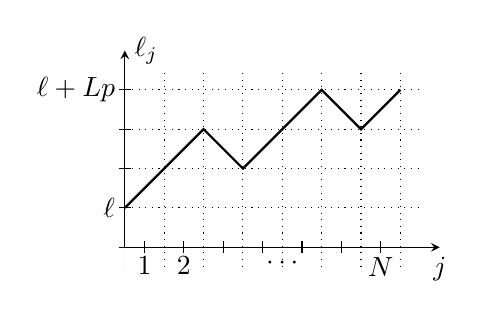
\begin{tikzpicture}[>=stealth]
     \draw[scale=0.5,thick] (0,0)--(2,2)--(3,1)--(5,3)--(6,2)--(7,3);
           
     \draw[<->] (0,2) -- (0,-0.5) -- (4,-0.5);
     \foreach \x in {0.25,0.75,...,3.25}
       \draw[xshift=\x cm,yshift=-0.5cm] (0,-0.075)--(0,0.075);
     
    \foreach \y in {-0.5,0,...,1.5}
       \draw[yshift=\y cm] (-0.075,0)--(0.075,0);
 
    \draw (0.25,-0.5) node[below] {$1$};
    \draw (0.75,-0.5) node[below] {$2$};
    \draw (2,-0.5) node[below] {$\cdots$};
    \draw (3.25,-0.5) node[below] {$N$};
    \draw (4,-0.5) node[below] {$j$};
    \draw (0,0) node [left] {$\ell$};
    \draw (0,1.5) node [left] {$\ell+Lp$};
    \draw (0,2) node [right] {$\ell_j$};
    \clip[scale=0.5] (0,-1.5) rectangle (7.5,3.5);
    \draw[scale=0.5,dotted] (-1,-2) grid (8,5);
  \end{tikzpicture}
}
  
\end{texexample}




%\begin{texexample}{Example}{}
%\newcommand{\ud}{\ensuremath \mathop{}\!\mathrm{d}}
%\(z=2\sin x\mathrm{d}x\) and \(z=2\sin x\ud x\)
%
%
%\newcommand{\ud}{\mathop{}\!\mathrm{d}}
%\bigskip
%
%It uses an empty operator and eliminates the space
%on its left with |\!|.
%
%Note the difference between
%
%\[z=2\sin x\mathrm{d}x  \]
%
%\[z=2\sin x\ud x\]
%
%where the diffrential is obtained respectively with
%|\mathrm{d}| and |\ud|.
%\end{texexample}




\subsubsection{God is in the details}

Sometimes you will be faced with small decisions for which the Journal style manual might not have an answer for you or the journal Editor might have a different opinion to yours. One such question is if one needs to insert the thousand separator in coefficients.

\[
\operatorname{erf}^{-1}(z)=\tfrac{1}{2}\sqrt{\pi}\left (z+\frac{\pi}{12}z^3+\frac{7\pi^2}{480}z^5+\frac{127\pi^3}{40320}z^7+\frac{4369\pi^4}{5806080}z^9+\frac{34807\pi^5}{182476800}z^{11}+\cdots\right )
\]


\[
\operatorname{erf}^{-1}(z)=\tfrac{1}{2}\sqrt{\pi}\left (z+\frac{\pi}{12}z^3+\frac{7\pi^2}{480}z^5+\frac{127\pi^3}{40,320}z^7+\frac{4,369\pi^4}{5,806,080}z^9+\frac{34,807\pi^5}{182{,}476,800}z^{11}+\cdots\right )
\]

\[
\operatorname{erf}^{-1}(z)=\tfrac{1}{2}\sqrt{\pi}\left (z+\frac{\pi}{12}z^3+\frac{7\pi^2}{480}z^5+\frac{127\pi^3}{40{,}320}z^7+\frac{4{,}369\pi^4}{5{,}806{,}080}z^9+\frac{34{,}807\pi^5}{182{,}476{,}800}z^{11}+\cdots\right )
\]



\[
\operatorname{erf}^{-1}(z)=\tfrac{1}{2}\sqrt{\pi}\left (z+\frac{\pi}{12}z^3+\frac{7\pi^2}{480}z^5+\frac{127\pi^3}{40\thinspace 320}z^7+\frac{4\thinspace 369\pi^4}{5\thinspace 806\thinspace 080}z^9+\frac{34\thinspace 807\pi^5}{182\thinspace 476\thinspace 800}z^{11}+\cdots\right )
\]


If you type the commas watch out to put them in |{,}| otherwise \tex's algorithm will leave a space. See the difference below:

\[182{,}476{,}800 \]
\[182,476,800\]

It is interesting to note that Knuth believes that in equations this is unnecessary.
He is quoted in Typesetting Mathematics.


\begin{quotation}
But where Don wrote 1000000 they substituted
1,000,000. Don objected that although this might be justifed in text, his use is perfectly OK in a formula. Well then, they replied, write \(10^6\).
Fine, said, Don, but what do I do 
when the number is 1234567? The IEEE standard here is to insert spaces, thus: 1 234 567.
Don doesn't like this in formulae, but agrees that it may be useful in a high precision context, such as numerical tables. 
\end{quotation}



The following are extracts from his paper \textit{Johann Faulhaber and Sums of Powers}:\footnote{\url{http://www-cs-faculty.stanford.edu/~uno/papers/jfsp.tex.gz}}

{
\[\vcenter{\halign{$#$\hfil\ &$#$\hfil\cr
\Sigma n^{11}&=39916800{n+6\choose 12}+
19958400{n+5\choose 10}+3160080{n+4\choose 8}
+168960{n+3\choose 6}\cr
\noalign{\smallskip}
&\qquad\null+2046{n+2\choose 4}+{n+1\choose 2}\,;\cr
\noalign{\smallskip}
\Sigma n^{13}&=6227020800{n+7\choose 14}+3632428800{n+6\choose 12}+
726485760{n+5\choose 10}\cr
\noalign{\smallskip}
&\qquad\null+57657600{n+4\choose 8}
+1561560{n+3\choose 6}+8190{n+2\choose 4}+\binom{n+1}{2}\,.\cr}}\]
}

Also, note in the last equation the use of a period at the end. 
This is something that evokes strong opinions and flaming wars in fora. 
I am not too sure if I agree on the last one, but the way that Knuth writes 
is very clear and his equations in a way are paragraphs. 
In this case the use of a period is recommended.


\subsection{Punctuation}
\index{maths>typography>punctuation}

There are two schools of thought when it comes to punctuation, that is punctuation in display style formulae. Some authors (Beccari, 2007) argue it is not necessary, others that it is necessary and essential \footcite{guiggiani2008}. Mermin \footcite{mermin89} strongly argued in his third rule that:  `The
Math Is Prose rule simply says: End
a displayed equation with a punctuation
mark. It is implicit in this
statement that the absence of a punctuation
mark is itself a degenerate
form of punctuation that, like periods,
commas or semicolons, can be used
provided it makes sense.''

The authors of this article believe that equations, both in display and text style, are part of the argumentation
and so punctuation should be used to help the reader. An example of good use of punctuation is:


Since
\[ a=b \]
and
\[ b=c,\]
it is proven that
\[ a =c. \]

It is extremely unusual to find an equation end with a question mark but here is one. What is 
\[ a = d^2\mathrm{?} \]

If you do put a question mark or an exclamation mark and you are using unicode fonts,
you will need to use |\mathrm{?}| not to confuse it with the relevant symbols.

Most journals require that equations be punctuated, like normal text. Even if the author of the manuscript disagrees, probably the journal editor will add the punctuation.

Read your mathematical text aloud and introduce punctuation as if it was spelled in words rather than mathematical symbols. 

\subsection{Numbering Equations}
\index{maths>typography>equation numbering}

One question that you may face is the numbering of display equations. Early books used numbering sparingly, whereas many authors go overboard and number all the equations.

According to Knuth et al:\footnote{\url{http://tex.loria.fr/typographie/mathwriting.pdf}}
Numbering all displayed formulas is usually a bad idea; number the important ones only.

Halmos\footnote{\url{http://www.math.uh.edu/~tomforde/Books/Halmos-How-To-Write.pdf}} offers pretty much the same good advice,

\begin{latexquotation}
What about ``inequality (*)", or ``equation (7)", or ``formula (iii)"; should all displays be labelled or numbered? My answer is no. Reason: just as you shouldn't mention irrelevant assumptions or name irrelevant concepts, you also shouldn't attach irrelevant labels. Some small part of the reader's attention is attracted to the label, and some small part of his mind will wonder why the label is there. If there is a reason, then the wonder serves a healthy purpose by way of preparation, with no fuss, for a future reference to the same idea; if there is no reason, then the attention and the wonder were wasted.
\end{latexquotation}

Mermin's argues in his Good samaritan Rule: that it is distressing to having to hunt for an equation back in a manuscript for Eq. (2.46) not because your subsequent progress requires
you to inspect it in detail, but merely to find out what it is about so
you may know the principles that go into the construction of Eq. (7.38).
The Good Samaritan rule says: When referring to an equation identify it by
a phrase as well as a number. No compassionate and helpful person
would herald the arrival of Eq. (7.38) by saying "inserting (2.47) and (3.51)
into (5.13)..." when it is possible to say "inserting the form (2.47) of the
electric field $E$ and the Lindhard form (3.51) of the dielectric function $e$ into
the constitutive equation (5.13). To be sure, it's longer this way but much 
clearer\ldots'

For those that want only the equations that are referenced numbered the package \pkgname{autoref} can automate this. This is not included in this package due to conflicts with \pkgname{mathtools} and \pkgname{amsmath}.
\footnote{See also discussion at \protect\url{http://tex.stackexchange.com/questions/29267/which-equations-should-be numbered/49080\#49080}}

Now if you wish to argue about this is fine.

\section{Mathmode}

\tex is in \textit{mathmode} when it is reading mathematics. The |ifmmode| can be used to find out if \tex is in math mode. It denotes the start of an if-then-else control structure that tests whether \tex is currently in either math mode or display math mode. The |\else| part is optional. <TeX code 1> is processed if TeX is in one of the math modes, otherwise it is ignored. 
If the |\else| section is included and TeX is not in one of the math modes then \meta{TeX code 2} is processed; otherwise it is ignored.


\begin{texexample}{Calligraphic fonts}{ex:cal}

\newcommand{\Acal}{\ifmmode \mathcal{Acal} \else \(\mathcal{Acal}\) \fi}
The commandd efines a macro |\Acal| that can be used both in and out of math mode to typeset a calligraphy script A. 

This is a calligraphic {\Acal} or ({\Acal}).
\end{texexample}


\section{Useful packages}

Besides the main packages that we have discussed so far and which should be in everyone's toolbox, there are a number of other packages that you may find useful. One such package is the \pkgname{multienum}, which although not really a packaged specializing in mathematical typesetting, it provides an environment to set multiple equations, as in an exercise or exam.



\subsection{the multienum package}

The \docpkg{multienum} enables  the typestting of multiple equations on one line and numbering them, either with roman, arabic or alpha letters.

\emphasis{usepackage, multienum,begin,end,multienumerate}
\begin{teXXX}
\documentclass{article}
\usepackage{multienum}
\renewcommand{\regularlisti}{\setcounter{multienumi}{0}%
  \renewcommand{\labelenumi}%
  {\addtocounter{multienumi}{1}\alph{multienumi})}}
\begin{document}
\begin{multienumerate}[oddlist]
\mitemxxx{\(x^2 + y^2 = 1\)}{\(a + b = c\)}{\(r-x = y+z\)}
\mitemxxx{\(f - y = z\)}{\(a - b = 2d\)}{\(r+x = 2y-3z\)}
\end{multienumerate}
\end{document}
\end{teXXX}


\begin{multienumerate}[oddlist]
\mitemxxx{\(x^2 + y^2 = 1\)}{\(a + b = c\)}{\(r-x = y+z\)}
\end{multienumerate}
\begin{multienumerate}[evenlist]
\mitemxxx{\(f - y = z\)}{\(a - b = 2d\)}{\(r+x = 2y-3z\)}
\end{multienumerate}


\hrule

\bigskip

We can also enumerate the items using an even-only or odd only
counter.
\subsection*{Answers to Even-Numbered Exercises}
\begin{multienumerate}[evenlist]
\mitemxxxx{Not}{Linear}{Not}{Quadratic}
\mitemxxxo{Not}{Linear}{No; if $x=3$, then $y=-2$.}
\mitemxx{$(x_1,x_2)=(2+\frac{1}{3}t,t)$ or
$(s,3s-6)$}{$(x_1,x_2,x_3)=(2+\frac{5}{2}s-3t,s,t)$}
\mitemx{$(x_1,x_2,x_3,x_4)= (\frac{1}{4}+\frac{5}{4}s+\frac{3}{4}t-u,s,t,u)$
or $(s,t,u,\frac{1}{4}-s+\frac{5}{4}t+\frac{3}{4}u)$}
\mitemxxxx{$(2,-1,3)$}{None}{$(2,1,0,1)$}{$(0,0,0,0)$}
\end{multienumerate}
\bigskip



\newcommand\thecasestudylabel{Case Study}
\newenvironment{casestudy}[2][]{%
   \clearpage\par\leavevmode
   \addcontentsline{toc}{section}{\thecasestudylabel:  #1}
    \topline\vskip1.5pt
   {\noindent\large CASE STUDY\par}\vspace{3.5pt}
   \noindent\textsc{\large#1}\par
   \bigskip
   {#2}
   \medskip
   \topline
}{%
\vfill\bottomline}

\begin{casestudy}[The Riemann hypothesis.]{%
Typeset the text and the equations, shown below. Use a standard minimal to achieve it. Note the fraktur fonts. Text must all be as one paragraph.}

It is well known that the Riemann zeta function $\zeta(s)$ of a complex variable $s=\sigma+it$ is defined by
\[
\zeta(s)=\sum_{n=1}^{\infty}\frac{1}{n^{s}}
\]
for the real part $\mathfrak{R}(s)>1$ and its analytic continuation in the half plane $\sigma>0$ is
\begin{equation}\label{func:zeta}
\zeta(s)=\sum_{n=1}^{N}\frac{1}{n^{s}}-\frac{N^{1-s}}{1-s}-\frac{1}{2}N^{-s}
+s\int_{N}^{\infty}\frac{\frac{1}{2}-\{x\}}{x^{s+1}}dx
\end{equation}
for any integer $N\geq1$ and $\mathfrak{R}(s)>0$.
It extends to an analytic function in the whole complex plane except for having a simple pole at $s=1$. Trivially, $\zeta(-2n)=0$ for all positive integers. All other zeros of the Riemann zeta functions are called its nontrivial zeros.
\bottomline

\begin{teX}
It is well known that the Riemann zeta function $\zeta(s)$ of a complex variable $s=\sigma+it$ is defined by
\[
\zeta(s)=\sum_{n=1}^{\infty}\frac{1}{n^{s}}
\]
for the real part $\mathfrak{R}(s)>1$ and its analytic continuation in the half plane $\sigma>0$ is
\begin{equation}\label{func:zeta}
\zeta(s)=\sum_{n=1}^{N}\frac{1}{n^{s}}-\frac{N^{1-s}}{1-s}-\frac{1}{2}N^{-s}
+s\int_{N}^{\infty}\frac{\frac{1}{2}-\{x\}}{x^{s+1}}dx
\end{equation}
for any integer $N\geq1$ and $\mathfrak{R}(s)>0$.
It extends to an analytic function in the whole complex plane except for having a simple pole at $s=1$. Trivially, $\zeta(-2n)=0$ for all positive integers. All other zeros of the Riemann zeta functions are called its nontrivial zeros.
\end{teX}

Please note that the maths and the text, are typed as a single block. Do not leave any spaces in between. We have used |\mathfrak| for the fraktur font. We have also used $it$ for the imaginary part. This would depend on the style used in your field. 
\end{casestudy}

\clearpage
\section{Gather}

\begin{docEnvironment}{gather}{}
This is like a multi line environment with no special horizontal alignment. All rows
are centered and can have an own equation number:
\end{docEnvironment}

\begin{texexample}{Gather}{ex:gather}
\begingroup
\def\O{\mathcal{O}}
\begin{gather}
 \O,\O(E_4),\O(E_2),\O(H-E_3-E_5),\O(H-E_3),\O(H-E_5),\\ 
\O(2H-E_1-E_3-E_5-E_6),\O(2H-E_1-E_3-E_5),\O(2H-E_3-E_5-E_6).
\end{gather}

So lautet der Beweis des Satzes $2 \times 2 = 4$:
\begin{gather}
(\Omega^{\nu})^{\mu}{}'x = \Omega^{\nu \times \mu}{}'x \text{ Def.}\\
%\begin{split}
\Omega^{2 \times 2}{}'x = (\Omega^{2})^{2}{}'x = (\Omega^{2})^{1 + 1}{}'x = \Omega^{2}{}'\Omega^{2}{}'x = \Omega^{1 + 1}{}'\Omega^{1 + 1}{}'x\nonumber \\
= (\Omega'\Omega)'(\Omega'\Omega)'x = \Omega'\Omega'\Omega'\Omega'x = \Omega^{1 + 1 + 1 + 1}{}'x = \Omega^{4}{}'x.
%\end{split}
\end{gather}


\begin{gather*}
  x = \Omega^{0}{}' x \text{ Def.\ and}\\
  \Omega'\Omega^{\nu}{}'x = \Omega^{\nu+1}{}'x \text{ Def.}
\end{gather*}
\begin{equation}
  x = \Omega^{0}{}' x \text{ Def.\ and}\\
\Omega'\Omega^{\nu}{}'x = \Omega^{\nu+1}{}'x \text{ Def.}
\end{equation}
\endgroup
\end{texexample}


\section{How to number equations either to the left or right?}
\label{eqnochange}

\latexe uses Plain TeX \docAuxCommand{eqno} and \docAuxCommand{leqno} to place the equation number either to the left or the right of the equation. The placement is done automatically and the recommended way is to set this through the documentclass declaration at the start of the document. This can also be set manually later on through the above control sequences, as shown in the Example~\ref{ex:eqno}.

\begin{texexample}{Left or right numbering}{ex:eqno}
\makeatletter
\[ a = b + x^2 \eqno \@eqnnum \]
or at left
\[ a = b + x^2 \leqno \@eqnnum \]
\makeatother
\end{texexample}


%\meaning\text

%\chapter{Unicode Math}
\tcbdocmarginnote{N 29-06-2018}
Unicode contains separate codepoints for most if not all variations of alphabet
shape one may wish to use in mathematical notation. The complete list is shown
in table 5. Some of these have been covered in the previous sections.
The math font switching commands do not nest; therefore if you want sans
serif bold, you must write |\mathbfsf{...}| rather than |\mathbf{\mathsf{...}}|.
This may change in the future.

\section{Unicode maths font setup}

The promise of Unicode is that all symbols and alphabetic variants are in one font. The \pkgname{unicode-math}
maps all the available unicode math characters of a math font to respective \latex commands. If you have patience you can actually input them directly from the keyboard rather than in commands.

The best advice that I can give you is to read the \pkgname{unicode-math} carefully. 

\begin{docCommand} {setmathfont} { \oarg{range=\meta{unicode range}, \meta{font features } } \marg{font name} }
In many cases using one font might not be adequate. Specific Unicode ranges can be assigned to separate fonts.
\end{docCommand}

\subsection{Control over maths alphabets}

\subsection{Math `versions'}

\subsection{Maths input}

\subsection{Math `style'}

\subsubsection{Bold style}

Similar as in the previous section, ISO standards differ somewhat to \tex’s conventions
(and classical typesetting) for ‘boldness’ in mathematics. In the past, it has
been customary to use bold upright letters to denote things like vectors and matrices.


$$\boldsymbol{\omega} \times \mathbf{T} = \mathbf{T'}$$

$$\mathbf{\omega} = {1\over 2}\kappa \mathbf{B} + {1\over 2}(\kappa \mathbf{B} + \tau \mathbf{T}) + {1\over 2}\tau \mathbf{T} = \kappa \mathbf{B} + \tau \mathbf{T}
$$

\[
\mathbf{e} = \frac{\mathbf{A}}{m k} = \frac{1}{m k}(\mathbf{p} \times \mathbf{L})
\]

\subsubsection{Sans serif style}

\subsubsection{Blackboard or double-struck}



\subsubsection{Caligraphic and Script variants}



\section{Growing and non-growing accents}

This are the most problematic with Unicode fonts.

%%%%%%%% INPUT INTEGRAL FILES %%%%%%%%%%
%%%%%%%%%%%%%%%%%%%%%%%%%%%%%%%
 %% Too many errors here need to revisit.
 \subsection{Delimiters}
 \begin{multicols}{2}
% \showmbrace/{002F}{}
% \showlbrace({0028}{}
% \showlbrace[{005B}{}
% \showlbrace\lbrace{007B}{}
% \showmbrace\backslash{005C}{}
% \showrbrace){0029}{}
% \showrbrace]{005D}{}
% \showrbrace\rbrace{007D}{}
% \showlbrace\lceil{2308}{}
% \showlbrace\lfloor{230A}{}
% \showlbrace\lmoustache{23B0}{*}
% \showlbrace\lbrbrak{2772}{*}
% \showlbrace\lBrack{27E6}{*}
% \showlbrace\langle{27E8}{}, \cmd<
% \showlbrace\lAngle{27EA}{*}
% \showlbrace\lgroup{27EE}{*}
% \showlbrace\lBrace{2983}{*}
% \showlbrace\lParen{2985}{*}
% \showrbrace\rceil{2309}{}
 %\showrbrace\rfloor{230B}{}
% \showrbrace\rmoustache{23B1}{*}
% \showrbrace\rbrbrak{2773}{*}
% \showrbrace\rBrack{27E7}{*}
% \showrbrace\rangle{27E9}{}, \cmd>
% \showrbrace\rAngle{27EB}{*}
% \showrbrace\rgroup{27EF}{*}
 %\showrbrace\rBrace{2984}{*}
% \showrbrace\rParen{2986}{*}
 \end{multicols}

 \begin{multicols}{2}
% \showmbrace\vert{007C}{}, \cmd|
 \showmbrace\Vert{2016}{*}, \cmd\|
 \showmbrace\Vvert{2980}{}
 \showmbrace\uparrow{2191}{}
 \showmbrace\downarrow{2193}{}
 \showmbrace\updownarrow{2195}{}
 \showmbrace\Uparrow{21D1}{}
 \showmbrace\Downarrow{21D3}{}
 \showmbrace\Updownarrow{21D5}{}
% \showmbrace\Uuparrow{290A}{*}
% \showmbrace\Ddownarrow{290B}{*}
% \showmbrace\UUparrow{27F0}{*}
% \showmbrace\DDownarrow{27F1}{*}
% \showmbrace\arrowvert{XXXX}{}
% \showmbrace\Arrowvert{XXXX}{}
% \showmbrace\bracevert{XXXX}{*}
 \end{multicols}

 \subsection{Other bracess}
 \begin{multicols}{2}
 \showsymbol\ulcorner{231C}{*}
 \showsymbol\urcorner{231D}{*}
 \showsymbol\llcorner{231E}{*}
 \showsymbol\lrcorner{231F}{*}
 \showsymbol\Lbrbrak{27EC}{*}
 \showsymbol\Rbrbrak{27ED}{*}
 \showsymbol\llparenthesis{2987}{*}
 \showsymbol\rrparenthesis{2988}{*}
 \showsymbol\llangle{2989}{*}
 \showsymbol\rrangle{298A}{*}
 \showsymbol\lbrackubar{298B}{*}
 \showsymbol\rbrackubar{298C}{*}
 \showsymbol\lbrackultick{298D}{*}
 \showsymbol\rbracklrtick{298E}{*}
 \showsymbol\lbracklltick{298F}{*}
 \showsymbol\rbrackurtick{2990}{*}
 \showsymbol\langledot{2991}{*}
 \showsymbol\rangledot{2992}{*}
 \showsymbol\lparenless{2993}{*}
 \showsymbol\rparengtr{2994}{*}
 \showsymbol\Lparengtr{2995}{*}
 \showsymbol\Rparenless{2996}{*}
 \showsymbol\lblkbrbrak{2997}{*}
 \showsymbol\rblkbrbrak{2998}{*}
 \showsymbol\lvzigzag{29D8}{*}
 \showsymbol\rvzigzag{29D9}{*}
 \showsymbol\Lvzigzag{29DA}{*}
 \showsymbol\Rvzigzag{29DB}{*}
 \showsymbol\lcurvyangle{29FC}{*}
 \showsymbol\rcurvyangle{29FD}{*}
 \showsymbol\lbrbrak{2772}{*}
 \showsymbol\rbrbrak{2773}{*}
 \showsymbol\lbag{27C5}{*}
 \showsymbol\rbag{27C6}{*}
 \showsymbol\Lbrbrak{27EC}{*}
 \showsymbol\Rbrbrak{27ED}{*}
 \end{multicols}

 \section{Alphabetics}
 \begin{multicols}{2}
\showsymbolalpha\Gamma{0393}{}
\showsymbolalpha\Delta{0394}{}
\showsymbolalpha\Theta{0398}{}
\showsymbolalpha\Lambda{039B}{}
\showsymbolalpha\Xi{039E}{}
\showsymbolalpha\Pi{03A0}{}
\showsymbolalpha\Sigma{03A3}{}
\showsymbolalpha\Upsilon{03A5}{}
\showsymbolalpha\Phi{03A6}{}
\showsymbolalpha\Psi{03A8}{}
\showsymbolalpha\Omega{03A9}{}
\showsymbolalpha\alpha{03B1}{}
\showsymbolalpha\beta{03B2}{}
\showsymbolalpha\gamma{03B3}{}
\showsymbolalpha\delta{03B4}{}
\showsymbolalpha\epsilon{03B5}{}
\showsymbolalpha\zeta{03B6}{}
\showsymbolalpha\eta{03B7}{}
\showsymbolalpha\theta{03B8}{}
\showsymbolalpha\iota{03B9}{}
\showsymbolalpha\kappa{03BA}{}
\showsymbolalpha\lambda{03BB}{}
\showsymbolalpha\mu{03BC}{}
\showsymbolalpha\nu{03BD}{}
\showsymbolalpha\xi{03BE}{}
\showsymbolalpha\pi{03C0}{}
\showsymbolalpha\rho{03C1}{}
\showsymbolalpha\sigma{03C3}{}
\showsymbolalpha\tau{03C4}{}
\showsymbolalpha\upsilon{03C5}{}
\showsymbolalpha\phi{03D5}{}
\showsymbolalpha\chi{03C7}{}
\showsymbolalpha\psi{03C8}{}
\showsymbolalpha\omega{03C9}{}
\showsymbolalpha\varepsilon{03F5}{}
\showsymbolalpha\vartheta{03D1}{}
\showsymbolalpha\varpi{03D6}{}
\showsymbolalpha\varrho{03F1}{}
\showsymbolalpha\varsigma{03C2}{}
\showsymbolalpha\varphi{03C6}{}
\showsymbolalpha\nabla{2207}{}
\showsymbolalpha\partial{2202}{}
\showsymbolalpha\imath{1D6A4}{}
\showsymbolalpha\jmath{1D6A5}{}
 \end{multicols}
% \subsection{Accents}
 \begin{multicols}{2}
 \showaccent\grave{0300}{}
 \showaccent\acute{0301}{}
 \showaccent\hat{0302}{}
 \showaccent\tilde{0303}{}
 \showaccent\bar{0304}{}
 \showaccent\breve{0306}{}
 \showaccent\dot{0307}{}
 \showaccent\ddot{0308}{}
 \showaccent\ovhook{0309}{}
 \showaccent\mathring{030A}{}
 \showaccent\check{030C}{}
 \showaccent\candra{0310}{}
 \showaccent\oturnedcomma{0312}{}
 \showaccent\ocommatopright{0315}{}
 \showaccent\droang{031A}{}
 \showaccent\leftharpoonaccent{20D0}{}
 \showaccent\rightharpoonaccent{20D1}{}
 %\showaccent\leftarrowaccent{20D6}{}
 \showaccent\vec{20D7}{}, \cmd\rightarrowaccent
 %\showaccent\leftrightarrowaccent{20E1}{}
 \showaccent\dddot{20DB}{}
 \showaccent\ddddot{20DC}{}
 \showaccent\annuity{20E7}{}
 \showaccent\widebridgeabove{20E9}{}
 \showaccent\asteraccent{20F0}{}
 \end{multicols}

 \begin{multicols}{2}
 \showwideaccent\widehat{0302}{*}
 \showwideaccent\widetilde{0303}{*}
% \showwideaccent\widecheck{030C}{*}
 \showwideaccent\overleftarrow{20D6}{}
 \showwideaccent\overrightarrow{20D7}{}
 \showwideaccent\underrightarrow{20EF}{}
 \showwideaccent\underleftarrow{20EE}{}
 \showwideaccent\overleftrightarrow{20E1}{}
 \showwideaccent\underleftrightarrow{034D}{}
% \showwideaccent\overleftharpoon{20D0}{}
% \showwideaccent\overrightharpoon{20D1}{}
% \showwideaccent\underleftharpoon{20EC}{}
% \showwideaccent\underrightharpoon{20ED}{}
 \end{multicols}

 OpenType STIX fonts include a number of under accents that can be used in
 math mode, but \TeX\ does not support under accents natively so such glyphs
 can not be used directly. Under accents can be set using regular accents and
 commands like |\underaccent| from the \pkgname{accents} package, for example
 gives |\(\underaccent{\hat}{X}\)|. The
 \pkgname{undertilde} package provides |\utilde| for extensible under tilde
 accent \citep{undertilde}.
 
 
 % \subsection{Over and under brackets}
 \begin{multicols}{2}
 %\showover\overbracket{23B4}{} conflict mathtools consider remove mathtools for UNICODE
 \showover\overparen{23DC}{}
 \showover\overbrace{23DE}{}
 \showover\underbracket{23B5}{} %conflict mathtools?
 \showover\underparen{23DD}{}
 \showover\underbrace{23DF}{}
 \end{multicols}

 \subsection{Radicals}
 \begin{multicols}{2}
 \showaccent\sqrt{221A}{}
 \showaccent\longdivision{27CC}{*}
 \end{multicols}
 
 
 
 
 
 
 \subsection{Big operators}
 \begin{multicols}{2}
 \showop\Bbbsum{2140}{}
 \showop\prod{220F}{}
 \showop\coprod{2210}{}
 \showop\sum{2211}{}
 \showop\bigwedge{22C0}{}
 \showop\bigvee{22C1}{}
 \showop\bigcap{22C2}{}
 \showop\bigcup{22C3}{}
 \showop\leftouterjoin{27D5}{*}
 \showop\rightouterjoin{27D6}{*}
 \showop\fullouterjoin{27D7}{*}
 \showop\bigbot{27D8}{*}
 \showop\bigtop{27D9}{*}
 \showop\xsol{29F8}{*}
 \showop\xbsol{29F9}{*}
 \showop\bigodot{2A00}{*}
 \showop\bigoplus{2A01}{*}
 \showop\bigotimes{2A02}{*}
 \showop\bigcupdot{2A03}{*}
 \showop\biguplus{2A04}{*}
 \showop\bigsqcap{2A05}{*}
 \showop\bigsqcup{2A06}{*}
 \showop\conjquant{2A07}{*}
 \showop\disjquant{2A08}{*}
 \showop\bigtimes{2A09}{*}
 \showop\modtwosum{2A0A}{*}
 \showop\Join{2A1D}{*}
 \showop\bigtriangleleft{2A1E}{*}
 \showop\zcmp{2A1F}{*}
 \showop\zpipe{2A20}{*}
 \showop\zproject{2A21}{*}
 \showop\biginterleave{2AFC}{}
 \showop\bigtalloblong{2AFF}{*}
 \end{multicols}
 
 \section{General manipulations test.}
 
 Here are some examples using big operators

$$\sum_{n=s}^t C\cdot f(n) = C\cdot \sum_{n=s}^t f(n),$$ where ``'C'' is a constant

\[\sum_{n=s}^t f(n) + \sum_{n=s}^{t} g(n) = \sum_{n=s}^t \left[f(n) + g(n)\right]\] 

\[\sum_{n=s}^t f(n) - \sum_{n=s}^{t} g(n) = \sum_{n=s}^t \left[f(n) - g(n)\right]\] 

\[\sum_{n=s}^t f(n) = \sum_{n=s+p}^{t+p} f(n-p) \] 

\[\sum_{n\in B} f(n) = \sum_{m\in A} f(\sigma(m)),\] for a bijection σ from a finite set ``$A$'' onto a finite set ``$B$''; this generalizes the preceding formula.

\[\sum_{n=s}^j f(n) + \sum_{n=j+1}^t f(n) = \sum_{n=s}^t f(n)\] 

\[\sum_{i=k_0}^{k_1}\sum_{j=l_0}^{l_1} a_{i,j} = \sum_{j=l_0}^{l_1}\sum_{i=k_0}^{k_1} a_{i,j}\] 

\[\sum_{k\le j \le i\le n} a_{i,j} = \sum_{i=k}^n\sum_{j=k}^i a_{i,j} = \sum_{j=k}^n\sum_{i=j}^n a_{i,j}\] 


\[\sum_{n=0}^t f(2n) + \sum_{n=0}^t f(2n+1) = \sum_{n=0}^{2t+1} f(n)\] 

\[\sum_{n=0}^t \sum_{i=0}^{z-1} f(z\cdot n+i) = \sum_{n=0}^{z\cdot t+z-1} f(n)\] 

\[\sum_{i=s}^m\sum_{j=t}^n {a_i}{c_j} = \sum_{i=s}^m a_i \cdot \sum_{j=t}^n c_j\] 

\[\sum_{n=s}^t \ln f(n) = \ln \prod_{n=s}^t f(n)\] 

\[c^{\left[\sum_{n=s}^t f(n) \right]} = \prod_{n=s}^t c^{f(n)}\] 
 
 
 \section{Convergence criteria}
 
The product of positive real numbers

\[\prod_{n=1}^{\infty} a_n\]
converges to a nonzero real number if and only if the sum
\[\sum_{n=1}^{\infty} \log(a_n)\]
converges. This allows the translation of convergence criteria for infinite sums into convergence criteria for infinite products. The same criterion applies to products of arbitrary complex numbers (including negative reals) if log is understood as a fixed Complex logarithm which satisfies $\log(1) = 0$, with the proviso that the infinite product diverges when infinitely many ''$a_n$'' fall outside 
the domain of log, whereas finitely many such ''$a_n$'' can be ignored in the sum.

For products of reals in which each $a_n\ge1$, written as, for instance, $a_n=1+p_n$,
where $p_n\ge 0$, the bounds

\[1+\sum_{n=1}^{N} p_n \le \prod_{n=1}^{N} \left( 1 + p_n \right) \le \exp \left( \sum_{n=1}^{N}p_n \right)\]

show that the infinite product converges precisely if the infinite sum of the $p_n$ converges. This relies on the Monotone convergence theorem. More generally, the convergence of $\prod_{n=1}^\infty(1+p_n)$ is equivalent to the convergence of $\sum_{n=1}^\infty p_n$ 
%if ''p<sub>n</sub>'' are real or complex numbers such that <math>\sum_{n=1}^\infty|p_n|^2<+\infty\], since <math>\log(1+x)=x+O(x^2)\] in a neighbourhood of 0.
%
%If the series ''p''<sub>''n''</sub> diverges, then the sequence of partial products converges to zero as a sequence.  The infinite product is said to '''diverge to zero'''.
% 
 
 
 
 
 
 
 
 
%% Relations symbols from STIX font
%% 
  \subsection{Relations}
 \begin{multicols}{2}
% \showrelsymbol*{002A}{}, \cmd\ast
% \showrelsymbol:{003A}{}
 \showrelsymbol{\less}{003C}{}, \cmd\less
 \showrelsymbol{\equal}{003D}{}, \cmd\equal
 \showrelsymbol{\greater}{003E}{}, \cmd\greater
 \showrelsymbol\closure{2050}{*}
 %\showrelsymbol\vertoverlay{20D2}{}
 \showrelsymbol\leftarrow{2190}{}, \cmd\gets
 \showrelsymbol\uparrow{2191}{}
 \showrelsymbol\rightarrow{2192}{}, \cmd\to
 \showrelsymbol\downarrow{2193}{}
 \showrelsymbol\leftrightarrow{2194}{}
 \showrelsymbol\updownarrow{2195}{}
 \showrelsymbol\nwarrow{2196}{}
 \showrelsymbol\nearrow{2197}{}
 \showrelsymbol\searrow{2198}{}
 \showrelsymbol\swarrow{2199}{}
 \showrelsymbol\nleftarrow{219A}{}
 \showrelsymbol\nrightarrow{219B}{}
 \showrelsymbol\leftwavearrow{219C}{}
 \showrelsymbol\rightwavearrow{219D}{}
 \showrelsymbol\twoheadleftarrow{219E}{}
 \showrelsymbol\twoheaduparrow{219F}{}
 \showrelsymbol\twoheadrightarrow{21A0}{}
 \showrelsymbol\twoheaddownarrow{21A1}{}
 \showrelsymbol\leftarrowtail{21A2}{}
 \showrelsymbol\rightarrowtail{21A3}{}
 \showrelsymbol\mapsfrom{21A4}{}
 \showrelsymbol\mapsup{21A5}{}
 \showrelsymbol\mapsto{21A6}{}
 \showrelsymbol\mapsdown{21A7}{}
 \showrelsymbol\hookleftarrow{21A9}{}
 \showrelsymbol\hookrightarrow{21AA}{}
 \showrelsymbol\looparrowleft{21AB}{}
 \showrelsymbol\looparrowright{21AC}{}
 \showrelsymbol\leftrightsquigarrow{21AD}{}
 \showrelsymbol\nleftrightarrow{21AE}{}
 \showrelsymbol\downzigzagarrow{21AF}{}
 \showrelsymbol\Lsh{21B0}{}
 \showrelsymbol\Rsh{21B1}{}
 \showrelsymbol\Ldsh{21B2}{}
 \showrelsymbol\Rdsh{21B3}{}
 \showrelsymbol\curvearrowleft{21B6}{}
 \showrelsymbol\curvearrowright{21B7}{}
 \showrelsymbol\circlearrowleft{21BA}{}
 \showrelsymbol\circlearrowright{21BB}{}
 \showrelsymbol\leftharpoonup{21BC}{}
 \showrelsymbol\leftharpoondown{21BD}{}
 \showrelsymbol\upharpoonright{21BE}{}, \cmd\restriction
 \showrelsymbol\upharpoonleft{21BF}{}
 \showrelsymbol\rightharpoonup{21C0}{}
 \showrelsymbol\rightharpoondown{21C1}{}
 \showrelsymbol\downharpoonright{21C2}{}
 \showrelsymbol\downharpoonleft{21C3}{}
 \showrelsymbol\rightleftarrows{21C4}{}
 \showrelsymbol\updownarrows{21C5}{}
 \showrelsymbol\leftrightarrows{21C6}{}
 \showrelsymbol\leftleftarrows{21C7}{}
 \showrelsymbol\upuparrows{21C8}{}
 \showrelsymbol\rightrightarrows{21C9}{}
 \showrelsymbol\downdownarrows{21CA}{}
 \showrelsymbol\leftrightharpoons{21CB}{}
 \showrelsymbol\rightleftharpoons{21CC}{}
 \showrelsymbol\nLeftarrow{21CD}{}
 \showrelsymbol\nLeftrightarrow{21CE}{}
 \showrelsymbol\nRightarrow{21CF}{}
 \showrelsymbol\Leftarrow{21D0}{}
 \showrelsymbol\Uparrow{21D1}{}
 \showrelsymbol\Rightarrow{21D2}{}
 \showrelsymbol\Downarrow{21D3}{}
 \showrelsymbol\Leftrightarrow{21D4}{}
 \showrelsymbol\Updownarrow{21D5}{}
 \showrelsymbol\Nwarrow{21D6}{}
 \showrelsymbol\Nearrow{21D7}{}
 \showrelsymbol\Searrow{21D8}{}
 \showrelsymbol\Swarrow{21D9}{}
 \showrelsymbol\Lleftarrow{21DA}{*}
 \showrelsymbol\Rrightarrow{21DB}{*}
 \showrelsymbol\leftsquigarrow{21DC}{}
 \showrelsymbol\rightsquigarrow{21DD}{}, \cmd\leadsto
 \showrelsymbol\barleftarrow{21E4}{*}
 \showrelsymbol\rightarrowbar{21E5}{*}
 \showrelsymbol\circleonrightarrow{21F4}{*}
 \showrelsymbol\downuparrows{21F5}{}
 \showrelsymbol\rightthreearrows{21F6}{*}
 \showrelsymbol\nvleftarrow{21F7}{*}
 \showrelsymbol\nvrightarrow{21F8}{*}
 \showrelsymbol\nvleftrightarrow{21F9}{*}
 \showrelsymbol\nVleftarrow{21FA}{*}
 \showrelsymbol\nVrightarrow{21FB}{*}
 \showrelsymbol\nVleftrightarrow{21FC}{*}
 \showrelsymbol\leftarrowtriangle{21FD}{*}
 \showrelsymbol\rightarrowtriangle{21FE}{*}
 \showrelsymbol\leftrightarrowtriangle{21FF}{*}
 \showrelsymbol\in{2208}{}
 \showrelsymbol\notin{2209}{}
 \showrelsymbol\smallin{220A}{}
 \showrelsymbol\ni{220B}{}, \cmd\owns
 \showrelsymbol\nni{220C}{}
 \showrelsymbol\smallni{220D}{}
 \showrelsymbol\propto{221D}{}
 \showrelsymbol\varpropto{221D}{}
 \showrelsymbol\mid{2223}{}
 \showrelsymbol\shortmid{2223}{}
 \showrelsymbol\nmid{2224}{}
 \showrelsymbol\nshortmid{2224}{*}
 \showrelsymbol\parallel{2225}{}
 \showrelsymbol\shortparallel{2225}{*}
 \showrelsymbol\nparallel{2226}{}
 \showrelsymbol\nshortparallel{2226}{*}
 \showrelsymbol\Colon{2237}{}
 \showrelsymbol\dashcolon{2239}{}
 \showrelsymbol\dotsminusdots{223A}{}
 \showrelsymbol\kernelcontraction{223B}{}
 \showrelsymbol\sim{223C}{}
 \showrelsymbol\thicksim{223C}{}
 \showrelsymbol\backsim{223D}{}
 \showrelsymbol\nsim{2241}{}
 \showrelsymbol\eqsim{2242}{}
 \showrelsymbol\simeq{2243}{}
 \showrelsymbol\nsime{2244}{}
 \showrelsymbol\cong{2245}{}
 \showrelsymbol\simneqq{2246}{}
 \showrelsymbol\ncong{2247}{}
 \showrelsymbol\approx{2248}{}
 \showrelsymbol\thickapprox{2248}{}
 \showrelsymbol\napprox{2249}{}
 \showrelsymbol\approxeq{224A}{}
 \showrelsymbol\approxident{224B}{}
 \showrelsymbol\backcong{224C}{}
 \showrelsymbol\asymp{224D}{}
 \showrelsymbol\Bumpeq{224E}{}
 \showrelsymbol\bumpeq{224F}{}
 \showrelsymbol\doteq{2250}{}
 \showrelsymbol\Doteq{2251}{}, \cmd\doteqdot
 \showrelsymbol\fallingdotseq{2252}{}
 \showrelsymbol\risingdotseq{2253}{}
 \showrelsymbol\coloneq{2254}{}
 \showrelsymbol\eqcolon{2255}{}
 \showrelsymbol\eqcirc{2256}{}
 \showrelsymbol\circeq{2257}{}
 \showrelsymbol\arceq{2258}{}
 \showrelsymbol\wedgeq{2259}{}
 \showrelsymbol\veeeq{225A}{}
 \showrelsymbol\stareq{225B}{}
 \showrelsymbol\triangleq{225C}{}
 \showrelsymbol\eqdef{225D}{}
 \showrelsymbol\measeq{225E}{}
 \showrelsymbol\questeq{225F}{}
 \showrelsymbol\ne{2260}{}, \cmd\neq
 \showrelsymbol\equiv{2261}{}
 \showrelsymbol\nequiv{2262}{}
 \showrelsymbol\Equiv{2263}{}
 \showrelsymbol\leq{2264}{}, \cmd\le
 \showrelsymbol\geq{2265}{}, \cmd\ge
 \showrelsymbol\leqq{2266}{}
 \showrelsymbol\geqq{2267}{}
 \showrelsymbol\lneqq{2268}{}
 \showrelsymbol\lvertneqq{2268}{}
 \showrelsymbol\gneqq{2269}{}
 \showrelsymbol\gvertneqq{2269}{}
 \showrelsymbol\ll{226A}{}
 \showrelsymbol\gg{226B}{}
 \showrelsymbol\between{226C}{}
 \showrelsymbol\nasymp{226D}{}
 \showrelsymbol\nless{226E}{}
 \showrelsymbol\ngtr{226F}{}
 \showrelsymbol\nleq{2270}{}
 \showrelsymbol\ngeq{2271}{}
 \showrelsymbol\lesssim{2272}{}
 \showrelsymbol\gtrsim{2273}{}
 \showrelsymbol\nlesssim{2274}{}
 \showrelsymbol\ngtrsim{2275}{}
 \showrelsymbol\lessgtr{2276}{}
 \showrelsymbol\gtrless{2277}{}
 \showrelsymbol\nlessgtr{2278}{}
 \showrelsymbol\ngtrless{2279}{}
 \showrelsymbol\prec{227A}{}
 \showrelsymbol\succ{227B}{}
 \showrelsymbol\preccurlyeq{227C}{}
 \showrelsymbol\succcurlyeq{227D}{}
 \showrelsymbol\precsim{227E}{}
 \showrelsymbol\succsim{227F}{}
 \showrelsymbol\nprec{2280}{}
 \showrelsymbol\nsucc{2281}{}
 \showrelsymbol\subset{2282}{}
 \showrelsymbol\supset{2283}{}
 \showrelsymbol\nsubset{2284}{}
 \showrelsymbol\nsupset{2285}{}
 \showrelsymbol\subseteq{2286}{}
 \showrelsymbol\supseteq{2287}{}
 \showrelsymbol\nsubseteq{2288}{}
 \showrelsymbol\nsupseteq{2289}{}
 \showrelsymbol\subsetneq{228A}{}
 \showrelsymbol\varsubsetneq{228A}{*}
 \showrelsymbol\supsetneq{228B}{}
 \showrelsymbol\varsupsetneq{228B}{*}
 \showrelsymbol\sqsubset{228F}{}
 \showrelsymbol\sqsupset{2290}{}
 \showrelsymbol\sqsubseteq{2291}{}
 \showrelsymbol\sqsupseteq{2292}{}
 \showrelsymbol\vdash{22A2}{}
 \showrelsymbol\dashv{22A3}{}
 \showrelsymbol\assert{22A6}{}
 \showrelsymbol\models{22A7}{}
 \showrelsymbol\vDash{22A8}{}
 \showrelsymbol\Vdash{22A9}{}
 \showrelsymbol\Vvdash{22AA}{}
 \showrelsymbol\VDash{22AB}{}
 \showrelsymbol\nvdash{22AC}{}
 \showrelsymbol\nvDash{22AD}{}
 \showrelsymbol\nVdash{22AE}{}
 \showrelsymbol\nVDash{22AF}{}
 \showrelsymbol\prurel{22B0}{}
 \showrelsymbol\scurel{22B1}{}
 \showrelsymbol\vartriangleleft{22B2}{}
 \showrelsymbol\vartriangleright{22B3}{}
 \showrelsymbol\trianglelefteq{22B4}{}
 \showrelsymbol\trianglerighteq{22B5}{}
 \showrelsymbol\origof{22B6}{}
 \showrelsymbol\imageof{22B7}{}
 \showrelsymbol\multimap{22B8}{}
 \showrelsymbol\bowtie{22C8}{}
 \showrelsymbol\backsimeq{22CD}{}
 \showrelsymbol\Subset{22D0}{}
 \showrelsymbol\Supset{22D1}{}
 \showrelsymbol\pitchfork{22D4}{}
 \showrelsymbol\equalparallel{22D5}{}
 \showrelsymbol\lessdot{22D6}{}
 \showrelsymbol\gtrdot{22D7}{}
 \showrelsymbol\lll{22D8}{}, \cmd\llless
 \showrelsymbol\ggg{22D9}{}, \cmd\gggtr
 \showrelsymbol\lesseqgtr{22DA}{}
 \showrelsymbol\gtreqless{22DB}{}
 \showrelsymbol\eqless{22DC}{}
 \showrelsymbol\eqgtr{22DD}{}
 \showrelsymbol\curlyeqprec{22DE}{}
 \showrelsymbol\curlyeqsucc{22DF}{}
 \showrelsymbol\npreccurlyeq{22E0}{}
 \showrelsymbol\nsucccurlyeq{22E1}{}
 \showrelsymbol\nsqsubseteq{22E2}{}
 \showrelsymbol\nsqsupseteq{22E3}{}
 \showrelsymbol\sqsubsetneq{22E4}{*}
 \showrelsymbol\sqsupsetneq{22E5}{*}
 \showrelsymbol\lnsim{22E6}{}
 \showrelsymbol\gnsim{22E7}{}
 \showrelsymbol\precnsim{22E8}{}
 \showrelsymbol\succnsim{22E9}{}
 \showrelsymbol\nvartriangleleft{22EA}{}
 \showrelsymbol\nvartriangleright{22EB}{}
 \showrelsymbol\ntrianglelefteq{22EC}{}
 \showrelsymbol\ntrianglerighteq{22ED}{}
 \showrelsymbol\vdots{22EE}{}
 \showrelsymbol\adots{22F0}{}
 \showrelsymbol\ddots{22F1}{}
 \showrelsymbol\disin{22F2}{*}
 \showrelsymbol\varisins{22F3}{*}
 \showrelsymbol\isins{22F4}{*}
 \showrelsymbol\isindot{22F5}{*}
 \showrelsymbol\varisinobar{22F6}{}
 \showrelsymbol\isinobar{22F7}{*}
 \showrelsymbol\isinvb{22F8}{*}
 \showrelsymbol\isinE{22F9}{*}
 \showrelsymbol\nisd{22FA}{*}
 \showrelsymbol\varnis{22FB}{*}
 \showrelsymbol\nis{22FC}{*}
 \showrelsymbol\varniobar{22FD}{}
 \showrelsymbol\niobar{22FE}{*}
 \showrelsymbol\bagmember{22FF}{*}
 \showrelsymbol\frown{2322}{}
 \showrelsymbol\smallfrown{2322}{*}
 \showrelsymbol\smile{2323}{}
 \showrelsymbol\smallsmile{2323}{*}
 \showrelsymbol\APLnotslash{233F}{}
 \showrelsymbol\vartriangle{25B5}{*}
 \showrelsymbol\perp{27C2}{*}
 \showrelsymbol\bsolhsub{27C8}{}
 \showrelsymbol\suphsol{27C9}{}
 \showrelsymbol\upin{27D2}{*}
 \showrelsymbol\pullback{27D3}{*}
 \showrelsymbol\pushout{27D4}{*}
 \showrelsymbol\DashVDash{27DA}{*}
 \showrelsymbol\dashVdash{27DB}{*}
 \showrelsymbol\multimapinv{27DC}{*}
 \showrelsymbol\vlongdash{27DD}{*}
 \showrelsymbol\longdashv{27DE}{*}
 \showrelsymbol\cirbot{27DF}{*}
 \showrelsymbol\UUparrow{27F0}{*}
 \showrelsymbol\DDownarrow{27F1}{*}
 \showrelsymbol\acwgapcirclearrow{27F2}{*}
 \showrelsymbol\cwgapcirclearrow{27F3}{*}
 \showrelsymbol\rightarrowonoplus{27F4}{*}
 \showrelsymbol\longleftarrow{27F5}{*}
 \showrelsymbol\longrightarrow{27F6}{*}
 \showrelsymbol\longleftrightarrow{27F7}{*}
 \showrelsymbol\Longleftarrow{27F8}{*}
 \showrelsymbol\Longrightarrow{27F9}{*}
 \showrelsymbol\Longleftrightarrow{27FA}{*}
 \showrelsymbol\longmapsfrom{27FB}{*}
 \showrelsymbol\longmapsto{27FC}{*}
 \showrelsymbol\Longmapsfrom{27FD}{*}
 \showrelsymbol\Longmapsto{27FE}{*}
 \showrelsymbol\longrightsquigarrow{27FF}{*}
 \showrelsymbol\nvtwoheadrightarrow{2900}{*}
 \showrelsymbol\nVtwoheadrightarrow{2901}{*}
 \showrelsymbol\nvLeftarrow{2902}{*}
 \showrelsymbol\nvRightarrow{2903}{*}
 \showrelsymbol\nvLeftrightarrow{2904}{*}
 \showrelsymbol\twoheadmapsto{2905}{*}
 \showrelsymbol\Mapsfrom{2906}{*}
 \showrelsymbol\Mapsto{2907}{*}
 \showrelsymbol\downarrowbarred{2908}{*}
 \showrelsymbol\uparrowbarred{2909}{*}
 \showrelsymbol\Uuparrow{290A}{*}
 \showrelsymbol\Ddownarrow{290B}{*}
 \showrelsymbol\leftbkarrow{290C}{*}
 \showrelsymbol\rightbkarrow{290D}{*}
 \showrelsymbol\leftdbkarrow{290E}{*}, \cmd\dashleftarrow
 \showrelsymbol\dbkarow{290F}{*}, \cmd\dashrightarrow
 \showrelsymbol\drbkarow{2910}{*}
 \showrelsymbol\rightdotarrow{2911}{*}
 \showrelsymbol\baruparrow{2912}{*}
 \showrelsymbol\downarrowbar{2913}{*}
 \showrelsymbol\nvrightarrowtail{2914}{*}
 \showrelsymbol\nVrightarrowtail{2915}{*}
 \showrelsymbol\twoheadrightarrowtail{2916}{*}
 \showrelsymbol\nvtwoheadrightarrowtail{2917}{*}
 \showrelsymbol\nVtwoheadrightarrowtail{2918}{*}
 \showrelsymbol\lefttail{2919}{*}
 \showrelsymbol\righttail{291A}{*}
 \showrelsymbol\leftdbltail{291B}{*}
 \showrelsymbol\rightdbltail{291C}{*}
 \showrelsymbol\diamondleftarrow{291D}{*}
 \showrelsymbol\rightarrowdiamond{291E}{*}
 \showrelsymbol\diamondleftarrowbar{291F}{*}
 \showrelsymbol\barrightarrowdiamond{2920}{*}
 \showrelsymbol\nwsearrow{2921}{*}
 \showrelsymbol\neswarrow{2922}{*}
 \showrelsymbol\hknwarrow{2923}{*}
 \showrelsymbol\hknearrow{2924}{*}
 \showrelsymbol\hksearow{2925}{*}
 \showrelsymbol\hkswarow{2926}{*}
 \showrelsymbol\tona{2927}{*}
 \showrelsymbol\toea{2928}{*}
 \showrelsymbol\tosa{2929}{*}
 \showrelsymbol\towa{292A}{*}
 \showrelsymbol\rightcurvedarrow{2933}{*}
 \showrelsymbol\leftdowncurvedarrow{2936}{*}
 \showrelsymbol\rightdowncurvedarrow{2937}{*}
 \showrelsymbol\cwrightarcarrow{2938}{*}
 \showrelsymbol\acwleftarcarrow{2939}{*}
 \showrelsymbol\acwoverarcarrow{293A}{*}
 \showrelsymbol\acwunderarcarrow{293B}{*}
 \showrelsymbol\curvearrowrightminus{293C}{*}
 \showrelsymbol\curvearrowleftplus{293D}{*}
 \showrelsymbol\cwundercurvearrow{293E}{*}
 \showrelsymbol\ccwundercurvearrow{293F}{*}
 \showrelsymbol\acwcirclearrow{2940}{*}
 \showrelsymbol\cwcirclearrow{2941}{*}
 \showrelsymbol\rightarrowshortleftarrow{2942}{*}
 \showrelsymbol\leftarrowshortrightarrow{2943}{*}
 \showrelsymbol\shortrightarrowleftarrow{2944}{*}
 \showrelsymbol\rightarrowplus{2945}{*}
 \showrelsymbol\leftarrowplus{2946}{*}
 \showrelsymbol\rightarrowx{2947}{*}
 \showrelsymbol\leftrightarrowcircle{2948}{*}
 \showrelsymbol\twoheaduparrowcircle{2949}{*}
 \showrelsymbol\leftrightharpoonupdown{294A}{*}
 \showrelsymbol\leftrightharpoondownup{294B}{*}
 \showrelsymbol\updownharpoonrightleft{294C}{*}
 \showrelsymbol\updownharpoonleftright{294D}{*}
 \showrelsymbol\leftrightharpoonupup{294E}{*}
 \showrelsymbol\updownharpoonrightright{294F}{*}
 \showrelsymbol\leftrightharpoondowndown{2950}{*}
 \showrelsymbol\updownharpoonleftleft{2951}{*}
 \showrelsymbol\barleftharpoonup{2952}{*}
 \showrelsymbol\rightharpoonupbar{2953}{*}
 \showrelsymbol\barupharpoonright{2954}{*}
 \showrelsymbol\downharpoonrightbar{2955}{*}
 \showrelsymbol\barleftharpoondown{2956}{*}
 \showrelsymbol\rightharpoondownbar{2957}{*}
 \showrelsymbol\barupharpoonleft{2958}{*}
 \showrelsymbol\downharpoonleftbar{2959}{*}
 \showrelsymbol\leftharpoonupbar{295A}{*}
 \showrelsymbol\barrightharpoonup{295B}{*}
 \showrelsymbol\upharpoonrightbar{295C}{*}
 \showrelsymbol\bardownharpoonright{295D}{*}
 \showrelsymbol\leftharpoondownbar{295E}{*}
 \showrelsymbol\barrightharpoondown{295F}{*}
 \showrelsymbol\upharpoonleftbar{2960}{*}
 \showrelsymbol\bardownharpoonleft{2961}{*}
 \showrelsymbol\leftharpoonsupdown{2962}{*}
 \showrelsymbol\upharpoonsleftright{2963}{*}
 \showrelsymbol\rightharpoonsupdown{2964}{*}
 \showrelsymbol\downharpoonsleftright{2965}{*}
 \showrelsymbol\leftrightharpoonsup{2966}{*}
 \showrelsymbol\leftrightharpoonsdown{2967}{*}
 \showrelsymbol\rightleftharpoonsup{2968}{*}
 \showrelsymbol\rightleftharpoonsdown{2969}{*}
 \showrelsymbol\leftharpoonupdash{296A}{*}
 \showrelsymbol\dashleftharpoondown{296B}{*}
 \showrelsymbol\rightharpoonupdash{296C}{*}
 \showrelsymbol\dashrightharpoondown{296D}{*}
 \showrelsymbol\updownharpoonsleftright{296E}{*}
 \showrelsymbol\downupharpoonsleftright{296F}{*}
 \showrelsymbol\rightimply{2970}{*}
 \showrelsymbol\equalrightarrow{2971}{*}
 \showrelsymbol\similarrightarrow{2972}{*}
 \showrelsymbol\leftarrowsimilar{2973}{*}
 \showrelsymbol\rightarrowsimilar{2974}{*}
 \showrelsymbol\rightarrowapprox{2975}{*}
 \showrelsymbol\ltlarr{2976}{*}
 \showrelsymbol\leftarrowless{2977}{*}
 \showrelsymbol\gtrarr{2978}{*}
 \showrelsymbol\subrarr{2979}{*}
 \showrelsymbol\leftarrowsubset{297A}{*}
 \showrelsymbol\suplarr{297B}{*}
 \showrelsymbol\leftfishtail{297C}{*}
 \showrelsymbol\rightfishtail{297D}{*}
 \showrelsymbol\upfishtail{297E}{*}
 \showrelsymbol\downfishtail{297F}{*}
 \showrelsymbol\rtriltri{29CE}{*}
 \showrelsymbol\ltrivb{29CF}{*}
 \showrelsymbol\vbrtri{29D0}{*}
 \showrelsymbol\lfbowtie{29D1}{*}
 \showrelsymbol\rfbowtie{29D2}{*}
 \showrelsymbol\fbowtie{29D3}{*}
 \showrelsymbol\lftimes{29D4}{*}
 \showrelsymbol\rftimes{29D5}{*}
 \showrelsymbol\dualmap{29DF}{*}
 \showrelsymbol\lrtriangleeq{29E1}{*}
 \showrelsymbol\eparsl{29E3}{*}
 \showrelsymbol\smeparsl{29E4}{*}
 \showrelsymbol\eqvparsl{29E5}{*}
 \showrelsymbol\gleichstark{29E6}{*}
 \showrelsymbol\ruledelayed{29F4}{*}
 \showrelsymbol\veeonwedge{2A59}{*}
 \showrelsymbol\eqdot{2A66}{}
 \showrelsymbol\dotequiv{2A67}{}
 \showrelsymbol\equivVert{2A68}{*}
 \showrelsymbol\equivVvert{2A69}{*}
 \showrelsymbol\dotsim{2A6A}{}
 \showrelsymbol\simrdots{2A6B}{*}
 \showrelsymbol\simminussim{2A6C}{*}
 \showrelsymbol\congdot{2A6D}{}
 \showrelsymbol\asteq{2A6E}{}
 \showrelsymbol\hatapprox{2A6F}{}
 \showrelsymbol\approxeqq{2A70}{}
 \showrelsymbol\eqqsim{2A73}{}
 \showrelsymbol\Coloneq{2A74}{*}
 \showrelsymbol\eqeq{2A75}{*}
 \showrelsymbol\eqeqeq{2A76}{*}
 \showrelsymbol\ddotseq{2A77}{*}
 \showrelsymbol\equivDD{2A78}{*}
 \showrelsymbol\ltcir{2A79}{*}
 \showrelsymbol\gtcir{2A7A}{*}
 \showrelsymbol\ltquest{2A7B}{*}
 \showrelsymbol\gtquest{2A7C}{*}
 \showrelsymbol\leqslant{2A7D}{}
 \showrelsymbol\geqslant{2A7E}{}
 \showrelsymbol\lesdot{2A7F}{*}
 \showrelsymbol\gesdot{2A80}{*}
 \showrelsymbol\lesdoto{2A81}{*}
 \showrelsymbol\gesdoto{2A82}{*}
 \showrelsymbol\lesdotor{2A83}{*}
 \showrelsymbol\gesdotol{2A84}{*}
 \showrelsymbol\lessapprox{2A85}{*}
 \showrelsymbol\gtrapprox{2A86}{*}
 \showrelsymbol\lneq{2A87}{}
 \showrelsymbol\gneq{2A88}{}
 \showrelsymbol\lnapprox{2A89}{}
 \showrelsymbol\gnapprox{2A8A}{}
 \showrelsymbol\lesseqqgtr{2A8B}{*}
 \showrelsymbol\gtreqqless{2A8C}{*}
 \showrelsymbol\lsime{2A8D}{*}
 \showrelsymbol\gsime{2A8E}{*}
 \showrelsymbol\lsimg{2A8F}{*}
 \showrelsymbol\gsiml{2A90}{*}
 \showrelsymbol\lgE{2A91}{*}
 \showrelsymbol\glE{2A92}{*}
 \showrelsymbol\lesges{2A93}{*}
 \showrelsymbol\gesles{2A94}{*}
 \showrelsymbol\eqslantless{2A95}{}
 \showrelsymbol\eqslantgtr{2A96}{}
 \showrelsymbol\elsdot{2A97}{*}
 \showrelsymbol\egsdot{2A98}{*}
 \showrelsymbol\eqqless{2A99}{*}
 \showrelsymbol\eqqgtr{2A9A}{*}
 \showrelsymbol\eqqslantless{2A9B}{*}
 \showrelsymbol\eqqslantgtr{2A9C}{*}
 \showrelsymbol\simless{2A9D}{}
 \showrelsymbol\simgtr{2A9E}{}
 \showrelsymbol\simlE{2A9F}{*}
 \showrelsymbol\simgE{2AA0}{*}
 \showrelsymbol\Lt{2AA1}{*}
 \showrelsymbol\Gt{2AA2}{*}
 \showrelsymbol\partialmeetcontraction{2AA3}{*}
 \showrelsymbol\glj{2AA4}{*}
 \showrelsymbol\gla{2AA5}{*}
 \showrelsymbol\ltcc{2AA6}{*}
 \showrelsymbol\gtcc{2AA7}{*}
 \showrelsymbol\lescc{2AA8}{*}
 \showrelsymbol\gescc{2AA9}{*}
 \showrelsymbol\smt{2AAA}{*}
 \showrelsymbol\lat{2AAB}{*}
 \showrelsymbol\smte{2AAC}{*}
 \showrelsymbol\late{2AAD}{*}
 \showrelsymbol\bumpeqq{2AAE}{*}
 \showrelsymbol\preceq{2AAF}{}
 \showrelsymbol\npreceq{XXXX}{*}
 \showrelsymbol\succeq{2AB0}{}
 \showrelsymbol\nsucceq{XXXX}{*}
 \showrelsymbol\precneq{2AB1}{*}
 \showrelsymbol\succneq{2AB2}{*}
 \showrelsymbol\preceqq{2AB3}{*}
 \showrelsymbol\succeqq{2AB4}{*}
 \showrelsymbol\precneqq{2AB5}{*}
 \showrelsymbol\succneqq{2AB6}{*}
 \showrelsymbol\precapprox{2AB7}{*}
 \showrelsymbol\succapprox{2AB8}{*}
 \showrelsymbol\precnapprox{2AB9}{*}
 \showrelsymbol\succnapprox{2ABA}{*}
 \showrelsymbol\Prec{2ABB}{*}
 \showrelsymbol\Succ{2ABC}{*}
 \showrelsymbol\subsetdot{2ABD}{}
 \showrelsymbol\supsetdot{2ABE}{}
 \showrelsymbol\subsetplus{2ABF}{*}
 \showrelsymbol\supsetplus{2AC0}{*}
 \showrelsymbol\submult{2AC1}{*}
 \showrelsymbol\supmult{2AC2}{*}
 \showrelsymbol\subedot{2AC3}{*}
 \showrelsymbol\supedot{2AC4}{*}
 \showrelsymbol\subseteqq{2AC5}{}
 \showrelsymbol\nsubseteqq{XXXX}{*}
 \showrelsymbol\supseteqq{2AC6}{}
 \showrelsymbol\nsupseteqq{XXXX}{*}
 \showrelsymbol\subsim{2AC7}{*}
 \showrelsymbol\supsim{2AC8}{*}
 \showrelsymbol\subsetapprox{2AC9}{*}
 \showrelsymbol\supsetapprox{2ACA}{*}
 \showrelsymbol\subsetneqq{2ACB}{}
 \showrelsymbol\varsubsetneqq{2ACB}{*}
 \showrelsymbol\supsetneqq{2ACC}{}
 \showrelsymbol\varsupsetneqq{2ACC}{*}
 \showrelsymbol\lsqhook{2ACD}{}
 \showrelsymbol\rsqhook{2ACE}{}
 \showrelsymbol\csub{2ACF}{}
 \showrelsymbol\csup{2AD0}{}
 \showrelsymbol\csube{2AD1}{}
 \showrelsymbol\csupe{2AD2}{}
 \showrelsymbol\subsup{2AD3}{}
 \showrelsymbol\supsub{2AD4}{}
 \showrelsymbol\subsub{2AD5}{}
 \showrelsymbol\supsup{2AD6}{}
 \showrelsymbol\suphsub{2AD7}{}
 \showrelsymbol\supdsub{2AD8}{}
 \showrelsymbol\forkv{2AD9}{}
 \showrelsymbol\topfork{2ADA}{}
 \showrelsymbol\mlcp{2ADB}{}
 \showrelsymbol\forks{2ADC}{}
 \showrelsymbol\forksnot{2ADD}{}
 \showrelsymbol\shortlefttack{2ADE}{}
 \showrelsymbol\shortdowntack{2ADF}{}
 \showrelsymbol\shortuptack{2AE0}{}
 \showrelsymbol\vDdash{2AE2}{}
 \showrelsymbol\dashV{2AE3}{}
 \showrelsymbol\Dashv{2AE4}{}
 \showrelsymbol\DashV{2AE5}{}
 \showrelsymbol\varVdash{2AE6}{}
 \showrelsymbol\Barv{2AE7}{}
 \showrelsymbol\vBar{2AE8}{}
 \showrelsymbol\vBarv{2AE9}{}
 \showrelsymbol\barV{2AEA}{}
 \showrelsymbol\Vbar{2AEB}{}
 \showrelsymbol\Not{2AEC}{}
 \showrelsymbol\bNot{2AED}{}
 \showrelsymbol\revnmid{2AEE}{}
 \showrelsymbol\cirmid{2AEF}{}
 \showrelsymbol\midcir{2AF0}{}
 \showrelsymbol\nhpar{2AF2}{}
 \showrelsymbol\parsim{2AF3}{}
 \showrelsymbol\lllnest{2AF7}{}
 \showrelsymbol\gggnest{2AF8}{}
 \showrelsymbol\leqqslant{2AF9}{}
 \showrelsymbol\geqqslant{2AFA}{}
 \showrelsymbol\circleonleftarrow{2B30}{*}
 \showrelsymbol\leftthreearrows{2B31}{*}
 \showrelsymbol\leftarrowonoplus{2B32}{*}
 \showrelsymbol\longleftsquigarrow{2B33}{*}
 \showrelsymbol\nvtwoheadleftarrow{2B34}{*}
 \showrelsymbol\nVtwoheadleftarrow{2B35}{*}
 \showrelsymbol\twoheadmapsfrom{2B36}{*}
 \showrelsymbol\twoheadleftdbkarrow{2B37}{*}
 \showrelsymbol\leftdotarrow{2B38}{*}
 \showrelsymbol\nvleftarrowtail{2B39}{*}
 \showrelsymbol\nVleftarrowtail{2B3A}{*}
 \showrelsymbol\twoheadleftarrowtail{2B3B}{*}
 \showrelsymbol\nvtwoheadleftarrowtail{2B3C}{*}
 \showrelsymbol\nVtwoheadleftarrowtail{2B3D}{*}
 \showrelsymbol\leftarrowx{2B3E}{*}
 \showrelsymbol\leftcurvedarrow{2B3F}{*}
 \showrelsymbol\equalleftarrow{2B40}{*}
 \showrelsymbol\bsimilarleftarrow{2B41}{*}
 \showrelsymbol\leftarrowbackapprox{2B42}{*}
 \showrelsymbol\rightarrowgtr{2B43}{*}
 \showrelsymbol\rightarrowsupset{2B44}{*}
 \showrelsymbol\LLeftarrow{2B45}{*}
 \showrelsymbol\RRightarrow{2B46}{*}
 \showrelsymbol\bsimilarrightarrow{2B47}{*}
 \showrelsymbol\rightarrowbackapprox{2B48}{*}
 \showrelsymbol\similarleftarrow{2B49}{*}
 \showrelsymbol\leftarrowapprox{2B4A}{*}
 \showrelsymbol\leftarrowbsimilar{2B4B}{*}
 \showrelsymbol\rightarrowbsimilar{2B4C}{*}
 \showrelsymbol\ngeqq{XXXX}{}
 \showrelsymbol\ngeqslant{XXXX}{}
 \showrelsymbol\nleqslant{XXXX}{}
 \showrelsymbol\nleqq{XXXX}{}
% \showrelsymbol\ncongdot{XXXX}{}
% \showrelsymbol\napproxeqq{XXXX}{}
% \showrelsymbol\nll{XXXX}{}
% \showrelsymbol\ngg{XXXX}{}
% \showrelsymbol\nsqsubset{XXXX}{}
% \showrelsymbol\nsqsupset{XXXX}{}
% \showrelsymbol\nBumpeq{XXXX}{}
% \showrelsymbol\nbumpeq{XXXX}{}
%\showrelsymbol\neqsim{XXXX}{}
 %\showrelsymbol\nvarisinobar{XXXX}{}
% \showrelsymbol\nvarniobar{XXXX}{}
% \showrelsymbol\neqslantless{XXXX}{}
 %\showrelsymbol\neqslantgtr{XXXX}{}
 \showrelsymbol\lhook{XXXX}{}
 \showrelsymbol\rhook{XXXX}{}
 \showrelsymbol\relbar{XXXX}{}
 \showrelsymbol\Relbar{XXXX}{}
 %\showrelsymbol\Rrelbar{XXXX}{*}
% \showrelsymbol\RRelbar{XXXX}{*}
 \showrelsymbol\mapsfromchar{XXXX}{}
 \showrelsymbol\mapstochar{XXXX}{}
 \end{multicols}
 %%% TODO HOW TO HANDLE BOTH LOCALLY
 %%%
 \subsection{Integrals}
 \label{integrals}
 Integrals come in two styles, the slanted versions shown below (|$\intsl$|,
 etc.)\ and right versions such as~|$\int$|. By default, the symbol names
 listed below will give you the slanted style, but if you specify the |int|
 package option, they will give you the corresponding right symbols.

 It is highly recommended that authors stick to the names below and use the
 |int| package option to choose a style globally for their document.
 However, in recognition of the fact that it might occasionally be necessary
 to mix the two styles, alternative names have been provided for all
 integrals. Append |sl| or || to the names below to request either the
 \emph{sl}anted or the \emph{}right variant. Thus, |$\intsl$| will always
 yield~|$\intsl$| and |$\int$| will always yield~|$\int$|, and similarly for
 the other integrals.
%
 \begin{multicols}{2}
 \integralsymbol\int{222B}{}
 \integralsymbol\iint{222C}{}
 \integralsymbol\iiint{222D}{}
 \integralsymbol\oint{222E}{}
 \integralsymbol\oiint{222F}{}
 \integralsymbol\oiiint{2230}{}
 \integralsymbol\intclockwise{2231}{}
 \integralsymbol\varointclockwise{2232}{}
 \integralsymbol\ointctrclockwise{2233}{}
 \integralsymbol\sumint{2A0B}{}
 \integralsymbol\iiiint{2A0C}{}
 \integralsymbol\intbar{2A0D}{}
 \integralsymbol\intBar{2A0E}{}
 \integralsymbol\fint{2A0F}{}
 \integralsymbol\cirfnint{2A10}{}
 \integralsymbol\awint{2A11}{}
 \integralsymbol\rppolint{2A12}{}
 \integralsymbol\scpolint{2A13}{}
 \integralsymbol\npolint{2A14}{}
 \integralsymbol\pointint{2A15}{}
 \integralsymbol\sqint{2A16}{}
 \integralsymbol\intlarhk{2A17}{}
 \integralsymbol\intx{2A18}{}
% \integralsymbol\intcapup{2A19}{}
 %\integralsymbol\intc{2A1A}{}
% \integralsymbol\intcup{2A1B}{}
 \integralsymbol\lowint{2A1C}{}
 \end{multicols}

\endinput



%%%%%%%%%%%%%%%%%%%%%%%%%%%%%%%
 \subsection{Ordinary symbols}
 \begin{multicols}{2}
 %\showsymbol\#{0023}{}
 %\showsymbol\mathdollar{0024}{}
 % \showsymbol\%{0025}{}
 %\showsymbol\&{0026}{}
% \showsymbol.{002E}{}
% \showsymbol/{002F}{}
% \showsymbol?{003F}{}
% \showsymbol@{0040}{}
 \showsymbol\backslash{005C}{}
 \showsymbol\mathsterling{00A3}{}
 \showsymbol\mathsection{00A7}{}
 \showsymbol\neg{00AC}{}, \cmd\lnot
 \showsymbol\mathparagraph{00B6}{}
 \showsymbol\eth{00F0}{}
 \showsymbol\Zbar{01B5}{*}
 \showsymbol\digamma{03DD}{}
 \showsymbol\varkappa{03F0}{}
 \showsymbol\backepsilon{03F6}{}
 \showsymbol\upbackepsilon{03F6}{}
 \showsymbol\enleadertwodots{2025}{}
 \showsymbol\mathellipsis{2026}{}
 \showsymbol\prime{2032}{}
 \showsymbol\dprime{2033}{}
 \showsymbol\trprime{2034}{}
 \showsymbol\backprime{2035}{}
 \showsymbol\backdprime{2036}{}
 \showsymbol\backtrprime{2037}{}
 \showsymbol\caretinsert{2038}{}
 \showsymbol\Exclam{203C}{}
 \showsymbol\hyphenbullet{2043}{*}
 \showsymbol\Question{2047}{}
 \showsymbol\qprime{2057}{}
 \showsymbol\enclosecircle{20DD}{}\indexmathcmd[Circles]{\enclosecircle}
 \showsymbol\enclosesquare{20DE}{*}
 \showsymbol\enclosediamond{20DF}{*}
 \showsymbol\enclosetriangle{20E4}{}
 \showsymbol\Eulerconst{2107}{}
 \showsymbol\hbar{210F}{*}
 \showsymbol\hslash{210F}{}
 \showsymbol\Im{2111}{}
 \showsymbol\ell{2113}{}
 \showsymbol\wp{2118}{}
 \showsymbol\Re{211C}{}
 \showsymbol\mho{2127}{}
 \showsymbol\turnediota{2129}{}
 \showsymbol\Angstrom{212B}{}
 \showsymbol\Finv{2132}{}
 \showsymbol\aleph{2135}{}
 \showsymbol\beth{2136}{}
 \showsymbol\gimel{2137}{}
 \showsymbol\daleth{2138}{}
 \showsymbol\Game{2141}{*}
 \showsymbol\sansLturned{2142}{*}
 \showsymbol\sansLmirrored{2143}{*}
 \showsymbol\Yup{2144}{*}
 \showsymbol\PropertyLine{214A}{*}
 \showsymbol\updownarrowbar{21A8}{}
 \showsymbol\linefeed{21B4}{}
 \showsymbol\carriagereturn{21B5}{}
 \showsymbol\barovernorthwestarrow{21B8}{}
 \showsymbol\barleftarrowrightarrowbar{21B9}{}
 \showsymbol\acwopencirclearrow{21BA}{}\indexmathcmd[Circles]{\acwopencirclearrow}
 \showsymbol\cwopencirclearrow{21BB}{}\indexmathcmd[Circles]{\cwopencirclearrow}
 \showsymbol\nHuparrow{21DE}{*}
 \showsymbol\nHdownarrow{21DF}{*}
 \showsymbol\leftdasharrow{21E0}{*}
 \showsymbol\updasharrow{21E1}{*}
 \showsymbol\rightdasharrow{21E2}{*}
 \showsymbol\downdasharrow{21E3}{*}
 \showsymbol\leftwhitearrow{21E6}{}
 \showsymbol\upwhitearrow{21E7}{}
 \showsymbol\rightwhitearrow{21E8}{}
 \showsymbol\downwhitearrow{21E9}{}
 \showsymbol\whitearrowupfrombar{21EA}{}
 \showsymbol\forall{2200}{}
 \showsymbol\complement{2201}{}
 \showsymbol\exists{2203}{}
 \showsymbol\nexists{2204}{}
 \showsymbol\varnothing{2205}{}
 \showsymbol\emptyset{2205}{}
 \showsymbol\increment{2206}{}
 \showsymbol\QED{220E}{*}
 \showsymbol\infty{221E}{}
 \showsymbol\rightangle{221F}{}
 \showsymbol\angle{2220}{}
 \showsymbol\measuredangle{2221}{}
 \showsymbol\sphericalangle{2222}{}
 \showsymbol\therefore{2234}{}
 \showsymbol\because{2235}{}
 \showsymbol\sinewave{223F}{}
 \showsymbol\top{22A4}{}
 \showsymbol\bot{22A5}{}
 \showsymbol\hermitmatrix{22B9}{}
 \showsymbol\measuredrightangle{22BE}{}
 \showsymbol\varlrtriangle{22BF}{}
 %\showsymbol\cdots{22EF}{} % TO FIX
 \showsymbol\diameter{2300}{*}
 \showsymbol\house{2302}{}
 \showsymbol\invnot{2310}{}
 \showsymbol\sqlozenge{2311}{*}
 \showsymbol\profline{2312}{*}
 \showsymbol\profsurf{2313}{*}
 \showsymbol\viewdata{2317}{*}
 \showsymbol\turnednot{2319}{}
 \showsymbol\varhexagonlrbonds{232C}{*}
 \showsymbol\conictaper{2332}{*}
 \showsymbol\topbot{2336}{}
 \showsymbol\APLnotbackslash{2340}{*}
 \showsymbol\APLboxupcaret{2353}{*}
 \showsymbol\APLboxquestion{2370}{*}
 \showsymbol\rangledownzigzagarrow{237C}{*}
 \showsymbol\hexagon{2394}{*}
 \showsymbol\bbrktbrk{23B6}{}
 \showsymbol\varcarriagereturn{23CE}{*}
 \showsymbol\obrbrak{23E0}{}
 \showsymbol\ubrbrak{23E1}{}
 \showsymbol\trapezium{23E2}{*}
 \showsymbol\benzenr{23E3}{*}
 \showsymbol\strns{23E4}{*}
 \showsymbol\fltns{23E5}{*}
 \showsymbol\accurrent{23E6}{*}
 \showsymbol\elinters{23E7}{*}
 \showsymbol\mathvisiblespace{2423}{}
 \showsymbol\circledR{24C7}{}
 \showsymbol\circledS{24C8}{}
 \showsymbol\mdlgblksquare{25A0}{*}, \cmd\blacksquare
 \showsymbol\mdlgwhtsquare{25A1}{*}, \cmd\square, \cmd\Box
 \showsymbol\squoval{25A2}{*}
 \showsymbol\blackinwhitesquare{25A3}{*}
 \showsymbol\squarehfill{25A4}{*}
 \showsymbol\squarevfill{25A5}{*}
 \showsymbol\squarehvfill{25A6}{*}
 \showsymbol\squarenwsefill{25A7}{*}
 \showsymbol\squareneswfill{25A8}{*}
 \showsymbol\squarecrossfill{25A9}{*}
 \showsymbol\smblksquare{25AA}{*}
 \showsymbol\smwhtsquare{25AB}{*}
 \showsymbol\hrectangleblack{25AC}{*}
 \showsymbol\hrectangle{25AD}{*}
 \showsymbol\vrectangleblack{25AE}{*}
 \showsymbol\vrectangle{25AF}{*}
 \showsymbol\parallelogramblack{25B0}{*}
 \showsymbol\parallelogram{25B1}{*}
 \showsymbol\bigblacktriangleup{25B2}{*}
 \showsymbol\blacktriangle{25B4}{*}
 \showsymbol\blacktriangleright{25B6}{*}
 \showsymbol\smallblacktriangleright{25B8}{*}
 \showsymbol\smalltriangleright{25B9}{*}
 \showsymbol\blackpointerright{25BA}{*}
 \showsymbol\whitepointerright{25BB}{*}
 \showsymbol\bigblacktriangledown{25BC}{*}
 \showsymbol\bigtriangledown{25BD}{}
 \showsymbol\blacktriangledown{25BE}{*}
 \showsymbol\triangledown{25BF}{*}
 \showsymbol\blacktriangleleft{25C0}{*}
 \showsymbol\smallblacktriangleleft{25C2}{*}
 \showsymbol\smalltriangleleft{25C3}{*}
 \showsymbol\blackpointerleft{25C4}{*}
 \showsymbol\whitepointerleft{25C5}{*}
 \showsymbol\mdlgblkdiamond{25C6}{*}
 \showsymbol\mdlgwhtdiamond{25C7}{*}
 \showsymbol\blackinwhitediamond{25C8}{*}
 \showsymbol\fisheye{25C9}{*}
 \showsymbol\mdlgwhtlozenge{25CA}{}, \cmd\lozenge, \\ \cmd\Diamond
 \showsymbol\dottedcircle{25CC}{*}
 \showsymbol\circlevertfill{25CD}{*}
 \showsymbol\bullseye{25CE}{*}
 \showsymbol\mdlgblkcircle{25CF}{*}
 \showsymbol\circlelefthalfblack{25D0}{*}
 \showsymbol\circlerighthalfblack{25D1}{*}
 \showsymbol\circlebottomhalfblack{25D2}{*}
 \showsymbol\circletophalfblack{25D3}{*}
 \showsymbol\circleurquadblack{25D4}{*}
 \showsymbol\blackcircleulquadwhite{25D5}{*}
 \showsymbol\blacklefthalfcircle{25D6}{*}
 \showsymbol\blackrighthalfcircle{25D7}{*}
 \showsymbol\inversebullet{25D8}{*}
 \showsymbol\inversewhitecircle{25D9}{*}
 \showsymbol\invwhiteupperhalfcircle{25DA}{*}
 \showsymbol\invwhitelowerhalfcircle{25DB}{*}
 \showsymbol\ularc{25DC}{*}
 \showsymbol\urarc{25DD}{*}
 \showsymbol\lrarc{25DE}{*}
 \showsymbol\llarc{25DF}{*}
 \showsymbol\topsemicircle{25E0}{*}
 \showsymbol\botsemicircle{25E1}{*}
 \showsymbol\lrblacktriangle{25E2}{*}
 \showsymbol\llblacktriangle{25E3}{*}
 \showsymbol\ulblacktriangle{25E4}{*}
 \showsymbol\urblacktriangle{25E5}{*}
 \showsymbol\circ{25E6}{}, \cmd\smwhtcircle
 \showsymbol\squareleftblack{25E7}{*}
 \showsymbol\squarerightblack{25E8}{*}
 \showsymbol\squareulblack{25E9}{*}
 \showsymbol\squarelrblack{25EA}{*}
 \showsymbol\trianglecdot{25EC}{}
 \showsymbol\triangleleftblack{25ED}{*}
 \showsymbol\trianglerightblack{25EE}{*}
 \showsymbol\lgwhtcircle{25EF}{*}
 \showsymbol\squareulquad{25F0}{*}
 \showsymbol\squarellquad{25F1}{*}
 \showsymbol\squarelrquad{25F2}{*}
 \showsymbol\squareurquad{25F3}{*}
 \showsymbol\circleulquad{25F4}{*}
 \showsymbol\circlellquad{25F5}{*}
 \showsymbol\circlelrquad{25F6}{*}
 \showsymbol\circleurquad{25F7}{*}
 \showsymbol\ultriangle{25F8}{*}
 \showsymbol\urtriangle{25F9}{*}
 \showsymbol\lltriangle{25FA}{*}
 \showsymbol\mdwhtsquare{25FB}{*}
 \showsymbol\mdblksquare{25FC}{*}
 \showsymbol\mdsmwhtsquare{25FD}{*}
 \showsymbol\mdsmblksquare{25FE}{*}
 \showsymbol\lrtriangle{25FF}{*}
 \showsymbol\bigstar{2605}{*}
 \showsymbol\bigwhitestar{2606}{*}
 \showsymbol\astrosun{2609}{}
 \showsymbol\danger{2621}{}
 \showsymbol\blacksmiley{263B}{}
 \showsymbol\sun{263C}{}
 \showsymbol\rightmoon{263D}{}
 \showsymbol\leftmoon{263E}{}
 \showsymbol\female{2640}{}
 \showsymbol\male{2642}{}
 \showsymbol\spadesuit{2660}{*}
 \showsymbol\heartsuit{2661}{*}
 \showsymbol\diamondsuit{2662}{*}
 \showsymbol\clubsuit{2663}{*}
 \showsymbol\varspadesuit{2664}{}
 \showsymbol\varheartsuit{2665}{}
 \showsymbol\vardiamondsuit{2666}{}
 \showsymbol\varclubsuit{2667}{}
 \showsymbol\quarternote{2669}{}
 \showsymbol\eighthnote{266A}{}
 \showsymbol\twonotes{266B}{}
 \showsymbol\flat{266D}{}
 \showsymbol\natural{266E}{}
 \showsymbol\sharp{266F}{}
 \showsymbol\acidfree{267E}{*}
 \showsymbol\dicei{2680}{}
 \showsymbol\diceii{2681}{}
 \showsymbol\diceiii{2682}{}
 \showsymbol\diceiv{2683}{}
 \showsymbol\dicev{2684}{}
 \showsymbol\dicevi{2685}{}
 \showsymbol\circledrightdot{2686}{}
 \showsymbol\circledtwodots{2687}{}
 \showsymbol\blackcircledrightdot{2688}{}
 \showsymbol\blackcircledtwodots{2689}{}
 \showsymbol\Hermaphrodite{26A5}{}
 \showsymbol\mdwhtcircle{26AA}{}
 \showsymbol\mdblkcircle{26AB}{}
 \showsymbol\mdsmwhtcircle{26AC}{}
 \showsymbol\neuter{26B2}{}
 \showsymbol\checkmark{2713}{}
 \showsymbol\maltese{2720}{}
 \showsymbol\circledstar{272A}{}
 \showsymbol\varstar{2736}{}
 \showsymbol\dingasterisk{273D}{}
 \showsymbol\draftingarrow{279B}{*}
 \showsymbol\threedangle{27C0}{*}
 \showsymbol\whiteinwhitetriangle{27C1}{*}
 \showsymbol\subsetcirc{27C3}{*}
 \showsymbol\supsetcirc{27C4}{*}
 \showsymbol\diagup{27CB}{*}
 \showsymbol\diagdown{27CD}{*}
 \showsymbol\diamondcdot{27D0}{*}
 \showsymbol\rdiagovfdiag{292B}{*}
 \showsymbol\fdiagovrdiag{292C}{*}
 \showsymbol\seovnearrow{292D}{*}
 \showsymbol\neovsearrow{292E}{*}
 \showsymbol\fdiagovnearrow{292F}{*}
 \showsymbol\rdiagovsearrow{2930}{*}
 \showsymbol\neovnwarrow{2931}{*}
 \showsymbol\nwovnearrow{2932}{*}
 \showsymbol\uprightcurvearrow{2934}{*}
 \showsymbol\downrightcurvedarrow{2935}{*}
 \showsymbol\mdsmblkcircle{2981}{*}
 \showsymbol\fourvdots{2999}{*}
 \showsymbol\vzigzag{299A}{*}
 \showsymbol\measuredangleleft{299B}{*}
 \showsymbol\rightanglesqr{299C}{*}
 \showsymbol\rightanglemdot{299D}{*}
 \showsymbol\angles{299E}{*}
 \showsymbol\angdnr{299F}{*}
 \showsymbol\gtlpar{29A0}{*}
 \showsymbol\sphericalangleup{29A1}{*}
 \showsymbol\turnangle{29A2}{*}
 \showsymbol\revangle{29A3}{*}
 \showsymbol\angleubar{29A4}{*}
 \showsymbol\revangleubar{29A5}{*}
 \showsymbol\wideangledown{29A6}{*}
 \showsymbol\wideangleup{29A7}{*}
 \showsymbol\measanglerutone{29A8}{*}
 \showsymbol\measanglelutonw{29A9}{*}
 \showsymbol\measanglerdtose{29AA}{*}
 \showsymbol\measangleldtosw{29AB}{*}
 \showsymbol\measangleurtone{29AC}{*}
 \showsymbol\measangleultonw{29AD}{*}
 \showsymbol\measangledrtose{29AE}{*}
 \showsymbol\measangledltosw{29AF}{*}
 \showsymbol\revemptyset{29B0}{*}
 \showsymbol\emptysetobar{29B1}{*}
 \showsymbol\emptysetocirc{29B2}{*}
 \showsymbol\emptysetoarr{29B3}{*}
 \showsymbol\emptysetoarrl{29B4}{*}
 \showsymbol\obot{29BA}{*}
 \showsymbol\olcross{29BB}{*}
 \showsymbol\odotslashdot{29BC}{*}
 \showsymbol\uparrowoncircle{29BD}{*}
 \showsymbol\circledwhitebullet{29BE}{*}
 \showsymbol\circledbullet{29BF}{*}
 \showsymbol\cirscir{29C2}{*}
 \showsymbol\cirE{29C3}{*}
 \showsymbol\boxonbox{29C9}{*}
 \showsymbol\triangleodot{29CA}{*}
 \showsymbol\triangleubar{29CB}{*}
 \showsymbol\triangles{29CC}{*}
 \showsymbol\iinfin{29DC}{*}
 \showsymbol\tieinfty{29DD}{*}
 \showsymbol\nvinfty{29DE}{*}
 \showsymbol\laplac{29E0}{*}
 \showsymbol\thermod{29E7}{*}
 \showsymbol\downtriangleleftblack{29E8}{*}
 \showsymbol\downtrianglerightblack{29E9}{*}
 \showsymbol\blackdiamonddownarrow{29EA}{*}
 \showsymbol\blacklozenge{29EB}{}
 \showsymbol\circledownarrow{29EC}{*}
 \showsymbol\blackcircledownarrow{29ED}{*}
 \showsymbol\errbarsquare{29EE}{*}
 \showsymbol\errbarblacksquare{29EF}{*}
 \showsymbol\errbardiamond{29F0}{*}
 \showsymbol\errbarblackdiamond{29F1}{*}
 \showsymbol\errbarcircle{29F2}{*}
 \showsymbol\errbarblackcircle{29F3}{*}
 \showsymbol\perps{2AE1}{}
 \showsymbol\topcir{2AF1}{}
 \showsymbol\squaretopblack{2B12}{}
 \showsymbol\squarebotblack{2B13}{}
 \showsymbol\squareurblack{2B14}{}
 \showsymbol\squarellblack{2B15}{}
 \showsymbol\diamondleftblack{2B16}{}
 \showsymbol\diamondrightblack{2B17}{}
 \showsymbol\diamondtopblack{2B18}{}
 \showsymbol\diamondbotblack{2B19}{}
 \showsymbol\dottedsquare{2B1A}{}
 \showsymbol\lgblksquare{2B1B}{}
 \showsymbol\lgwhtsquare{2B1C}{}
 \showsymbol\vysmblksquare{2B1D}{}
 \showsymbol\vysmwhtsquare{2B1E}{}
 \showsymbol\pentagonblack{2B1F}{}
 \showsymbol\pentagon{2B20}{}
 \showsymbol\varhexagon{2B21}{}
 \showsymbol\varhexagonblack{2B22}{}
 \showsymbol\hexagonblack{2B23}{}
 \showsymbol\lgblkcircle{2B24}{}
 \showsymbol\mdblkdiamond{2B25}{}
 \showsymbol\mdwhtdiamond{2B26}{}
 \showsymbol\mdblklozenge{2B27}{}
 \showsymbol\mdwhtlozenge{2B28}{}
 \showsymbol\smblkdiamond{2B29}{}
 \showsymbol\smblklozenge{2B2A}{}
 \showsymbol\smwhtlozenge{2B2B}{}
 \showsymbol\blkhorzoval{2B2C}{}
 \showsymbol\whthorzoval{2B2D}{}
 \showsymbol\blkvertoval{2B2E}{}
 \showsymbol\whtvertoval{2B2F}{}
 \showsymbol\medwhitestar{2B50}{}
 \showsymbol\medblackstar{2B51}{}
 \showsymbol\smwhitestar{2B52}{}
 \showsymbol\rightpentagonblack{2B53}{}
 \showsymbol\rightpentagon{2B54}{}
 \showsymbol\postalmark{3012}{}
 \showsymbol\hzigzag{3030}{}
 \showsymbol\Bbbk{1D55C}{}
 \showsymbol\bracevert{XXXX}{*}
 \end{multicols}

 \subsection{Binary operators}
 \index{binary operators}
 \begin{multicols}{2}
% \showsymbolbin+{000B}{}
 \showsymbolbin\pm{00B1}{}
 \showsymbolbin\cdotp{00B7}{}%?, \cmd\centerdot
 \showsymbolbin\times{00D7}{}
 \showsymbolbin\div{00F7}{}
 \showsymbolbin\dagger{2020}{}
 \showsymbolbin\ddagger{2021}{}
 \showsymbolbin\smblkcircle{2022}{}
 \showsymbolbin\fracslash{2044}{}
 \showsymbolbin\upand{214B}{}
% \showsymbolbin-{000D}{}
 \showsymbolbin\mp{2213}{}
 \showsymbolbin\dotplus{2214}{}
 \showsymbolbin\smallsetminus{2216}{}
 \showsymbolbin\ast{2217}{}
 \showsymbolbin\vysmwhtcircle{2218}{}
 \showsymbolbin\vysmblkcircle{2219}{}, {\small\cmd\bullet}
 \showsymbolbin\wedge{2227}{}, \cmd\land
 \showsymbolbin\vee{2228}{}, \cmd\lor
 \showsymbolbin\cap{2229}{}
 \showsymbolbin\cup{222A}{}
 \showsymbolbin\dotminus{2238}{}
 \showsymbolbin\invlazys{223E}{}
 \showsymbolbin\wr{2240}{}
 \showsymbolbin\cupleftarrow{228C}{}
 \showsymbolbin\cupdot{228D}{}
 \showsymbolbin\uplus{228E}{}
 \showsymbolbin\sqcap{2293}{}
 \showsymbolbin\sqcup{2294}{}
 \showsymbolbin\oplus{2295}{}
 \showsymbolbin\ominus{2296}{}
 \showsymbolbin\otimes{2297}{}
 \showsymbolbin\oslash{2298}{}
 \showsymbolbin\odot{2299}{}
 \showsymbolbin\circledcirc{229A}{}
 \showsymbolbin\circledast{229B}{}
 \showsymbolbin\circledequal{229C}{}
 \showsymbolbin\circleddash{229D}{}
 \showsymbolbin\boxplus{229E}{}
 \showsymbolbin\boxminus{229F}{}
 \showsymbolbin\boxtimes{22A0}{}
 \showsymbolbin\boxdot{22A1}{}
 \showsymbolbin\intercal{22BA}{}
 \showsymbolbin\veebar{22BB}{}
 \showsymbolbin\barwedge{22BC}{}
 \showsymbolbin\barvee{22BD}{}
 \showsymbolbin\diamond{22C4}{}, \cmd\smwhtdiamond
 \showsymbolbin\cdot{22C5}{*}
 \showsymbolbin\star{22C6}{}
 \showsymbolbin\divideontimes{22C7}{}
 \showsymbolbin\ltimes{22C9}{}
 \showsymbolbin\rtimes{22CA}{}
 \showsymbolbin\leftthreetimes{22CB}{}
 \showsymbolbin\rightthreetimes{22CC}{}
 \showsymbolbin\curlyvee{22CE}{}
 \showsymbolbin\curlywedge{22CF}{}
 \showsymbolbin\Cap{22D2}{}, \cmd\doublecap
 \showsymbolbin\Cup{22D3}{}, \cmd\doublecup
 \showsymbolbin\varbarwedge{2305}{*}
 \showsymbolbin\vardoublebarwedge{2306}{*}
 \showsymbolbin\obar{233D}{}
 \showsymbolbin\triangle{25B3}{}, \cmd\bigtriangleup
 \showsymbolbin\lhd{22B2}{}
 \showsymbolbin\rhd{22B3}{}
 \showsymbolbin\unlhd{22B4}{}
 \showsymbolbin\unrhd{22B5}{}
 \showsymbolbin\mdlgwhtcircle{25CB}{*}
 \showsymbolbin\boxbar{25EB}{*}
 \showsymbolbin\veedot{27C7}{*}
 \showsymbolbin\wedgedot{27D1}{*}
 \showsymbolbin\lozengeminus{27E0}{*}
 \showsymbolbin\concavediamond{27E1}{*}
 \showsymbolbin\concavediamondtickleft{27E2}{*}
 \showsymbolbin\concavediamondtickright{27E3}{*}
 \showsymbolbin\whitesquaretickleft{27E4}{*}
 \showsymbolbin\whitesquaretickright{27E5}{*}
 \showsymbolbin\typecolon{2982}{*}
 \showsymbolbin\circlehbar{29B5}{*}
 \showsymbolbin\circledvert{29B6}{}
 \showsymbolbin\circledparallel{29B7}{}
 \showsymbolbin\obslash{29B8}{}
 \showsymbolbin\operp{29B9}{*}
 \showsymbolbin\olessthan{29C0}{}
 \showsymbolbin\ogreaterthan{29C1}{}
 \showsymbolbin\boxdiag{29C4}{}
 \showsymbolbin\boxbslash{29C5}{}
 \showsymbolbin\boxast{29C6}{}
 \showsymbolbin\boxcircle{29C7}{}
 \showsymbolbin\boxbox{29C8}{*}
 \showsymbolbin\triangleserifs{29CD}{*}
 \showsymbolbin\hourglass{29D6}{*}
 \showsymbolbin\blackhourglass{29D7}{*}
 \showsymbolbin\shuffle{29E2}{*}
 \showsymbolbin\mdlgblklozenge{29EB}{*}
 \showsymbolbin\setminus{29F5}{*}
 \showsymbolbin\dsol{29F6}{*}
 \showsymbolbin\rsolbar{29F7}{*}
 \showsymbolbin\doubleplus{29FA}{*}
 \showsymbolbin\tripleplus{29FB}{*}
 \showsymbolbin\tplus{29FE}{*}
 \showsymbolbin\tminus{29FF}{*}
 \showsymbolbin\ringplus{2A22}{}
 \showsymbolbin\plushat{2A23}{}
 \showsymbolbin\simplus{2A24}{}
 \showsymbolbin\plusdot{2A25}{}
 \showsymbolbin\plussim{2A26}{}
 \showsymbolbin\plussubtwo{2A27}{}
 \showsymbolbin\plustrif{2A28}{*}
 \showsymbolbin\commaminus{2A29}{*}
 \showsymbolbin\minusdot{2A2A}{}
 \showsymbolbin\minusfdots{2A2B}{}
 \showsymbolbin\minusrdots{2A2C}{*}
 \showsymbolbin\opluslhrim{2A2D}{*}
 \showsymbolbin\oplusrhrim{2A2E}{*}
 \showsymbolbin\vectimes{2A2F}{*}
 \showsymbolbin\dottimes{2A30}{}
 \showsymbolbin\timesbar{2A31}{}
 \showsymbolbin\btimes{2A32}{}
 \showsymbolbin\smashtimes{2A33}{*}
 \showsymbolbin\otimeslhrim{2A34}{*}
 \showsymbolbin\otimesrhrim{2A35}{*}
 \showsymbolbin\otimeshat{2A36}{*}
 \showsymbolbin\Otimes{2A37}{*}
 \showsymbolbin\odiv{2A38}{*}
 \showsymbolbin\triangleplus{2A39}{*}
 \showsymbolbin\triangleminus{2A3A}{*}
 \showsymbolbin\triangletimes{2A3B}{*}
 \showsymbolbin\intprod{2A3C}{*}
 \showsymbolbin\intprodr{2A3D}{*}
 \showsymbolbin\fcmp{2A3E}{*}
 \showsymbolbin\amalg{2A3F}{}
 \showsymbolbin\capdot{2A40}{*}
 \showsymbolbin\uminus{2A41}{*}
 \showsymbolbin\barcup{2A42}{*}
 \showsymbolbin\barcap{2A43}{*}
 \showsymbolbin\capwedge{2A44}{*}
 \showsymbolbin\cupvee{2A45}{*}
 \showsymbolbin\cupovercap{2A46}{*}
 \showsymbolbin\capovercup{2A47}{*}
 \showsymbolbin\cupbarcap{2A48}{*}
 \showsymbolbin\capbarcup{2A49}{*}
 \showsymbolbin\twocups{2A4A}{*}
 \showsymbolbin\twocaps{2A4B}{*}
 \showsymbolbin\closedvarcup{2A4C}{*}
 \showsymbolbin\closedvarcap{2A4D}{*}
 \showsymbolbin\Sqcap{2A4E}{*}
 \showsymbolbin\Sqcup{2A4F}{*}
 \showsymbolbin\closedvarcupsmashprod{2A50}{*}
 \showsymbolbin\wedgeodot{2A51}{*}
 \showsymbolbin\veeodot{2A52}{*}
 \showsymbolbin\Wedge{2A53}{*}
 \showsymbolbin\Vee{2A54}{*}
 \showsymbolbin\wedgeonwedge{2A55}{*}
 \showsymbolbin\veeonvee{2A56}{*}
 \showsymbolbin\bigslopedvee{2A57}{*}
 \showsymbolbin\bigslopedwedge{2A58}{*}
 \showsymbolbin\wedgemidvert{2A5A}{*}
 \showsymbolbin\veemidvert{2A5B}{*}
 \showsymbolbin\midbarwedge{2A5C}{*}
 \showsymbolbin\midbarvee{2A5D}{*}
 \showsymbolbin\doublebarwedge{2A5E}{}
 \showsymbolbin\wedgebar{2A5F}{*}
 \showsymbolbin\wedgedoublebar{2A60}{*}
 \showsymbolbin\varveebar{2A61}{*}
 \showsymbolbin\doublebarvee{2A62}{*}
 \showsymbolbin\veedoublebar{2A63}{}
 \showsymbolbin\dsub{2A64}{*}
 \showsymbolbin\rsub{2A65}{*}
 \showsymbolbin\eqqplus{2A71}{}
 \showsymbolbin\pluseqq{2A72}{}
 \showsymbolbin\interleave{2AF4}{}
 \showsymbolbin\nhVvert{2AF5}{}
 \showsymbolbin\threedotcolon{2AF6}{}
 \showsymbolbin\trslash{2AFB}{}
 \showsymbolbin\sslash{2AFD}{}
 \showsymbolbin\talloblong{2AFE}{}
 \end{multicols}










%%% Check on why fonttable gives problems in Index
\parindent1em
\chapter{Symbols}

\section{Introduction}
\label{ch:comprehensivesymbols}

The \pkgname{phd} package, preloads a number of packages, to provide as
many symbols as possible irrespective of the \tex engine used. Many of these
symbols can easily be replaced by the use of \pkgname{fontspec} and if
the package is set to unicode math with the use of and suitable fonts Open Type Fonts. What follows has been largely copied from \emph{The Comprehensive List of \latexe Symbols}, which has been the authoritative publication, using almost all available symbols. 
The publication lists many symbols which I have dropped due to having exceeded the number of math alphabets allowed by \tex. 


With the newer engines \xetex \luatex you can now use any symbol you can imagine, but there is still room and advantages for using commands. It is at least for me faster than looking up a symbol's unicode character or trying it out with a screen keyboard (unless of course you are using a foreign language keyboard). 

The sections that follow describe the commands and packages that are
available, by simply including the \pkgname{phd} package. Most of the conflicts have been resolved and I am hoping that in the next version we will add some more symbols. 
Currently these are over 1500 as commands and in excess of 60,000 unicode glyphs, provided you have access to the fonts.\footnote{This document has been compiled using \luatex.}
  

\subsection{Reserved Symbols}
\tex has a number of symbols that need to be escaped, as they have 
special meanings during processing see Table~\vref{special-escapable} and also Chapter~\vref{ch:characters}.


\begin{symtable}{\latexe{} Escapable ``Special'' Characters}
\index{special characters=``special'' characters}
\index{escapable characters}
\index{underline}
\label{special-escapable}
\begin{tabular}{*6{ll@{\qqquad}}ll}
\K\$   & \K\%   & \K\_$\,^*$  & \Kp\}  & \K\&   & \K\#   & \Kp\{   \\
\end{tabular}
\end{symtable}

The \latexe kernel command \refCom{@sanitize} changes the catcode of these characters so they can be included in commands such as |\index|. In text just escape them with a (\textbackslash).


\begin{longsymtable}{Predefined \latexe{} Text-mode Commands}
\index{inequalities}
\index{tilde}
\index{underline}
\index{copyright}
\idxboth{dot}{symbols}
\index{dots (ellipses)} \index{ellipses (dots)}
\idxboth{legal}{symbols}
\label{text-predef}
\begin{longtable}{lll@{\qqquad}lll}
\indexTextcomp\textasciicircum$^*$    					& \indexTextcomp\textless                             \\
\indexTextcomp\textasciitilde$^*$     						& \indexTextcomp[\ltextordfeminine]\textordfeminine   \\
\indexTextcomp\textasteriskcentered   					& \indexTextcomp[\ltextordmasculine]\textordmasculine \\
\indexTextcomp{\textbackslash}          				    & \indexTextcomp\textparagraph$^\dag$                 \\
texbar                                              & \indexTextcomp\textperiodcentered                   \\
\indexTextcomp{textbraceleft}           $^\dag$   & \indexTextcomp\textquestiondown                     \\
\indexTextcomp\textbraceright$^\dag$  & \indexTextcomp\textquotedblleft                     \\
\indexTextcomp\textbullet             & \indexTextcomp\textquotedblright                    \\
\indexTextcomp[\ltextcopyright]\textcopyright$^\dag$
                          & \indexTextcomp\textquoteleft                        \\
\indexTextcomp\textdagger$^\dag$      & \indexTextcomp\textquoteright                       \\
\indexTextcomp\textdaggerdbl$^\dag$   & \indexTextcomp[\ltextregistered]\textregistered     \\
\indexTextcomp\textdollar$^\dag$      & \indexTextcomp\textsection$^\dag$                   \\
\indexTextcomp\textellipsis$^\dag$    & \indexTextcomp\textsterling$^\dag$                  \\
\indexTextcomp\textemdash             & \indexTextcomp[\ltexttrademark]\texttrademark       \\
\indexTextcomp\textendash             & \indexTextcomp\textunderscore$^\dag$                \\
\indexTextcomp\textexclamdown         & \indexTextcomp\textvisiblespace                     \\
\indexTextcomp\textgreater                                                      \\
\end{longtable}

\bigskip
\twosymbolmessage

\bigskip
\begin{tablenote}[*]
  \docAuxCommand{^} and
%  \cmdI[\string\~{}]{\~{}}\verb|{}| can be used instead of
  \docAuxCommand{textasciicircum} and \docAuxCommand{textasciitilde}.  See the
  discussion of ``\texttt{\textasciitilde}'' \vpageref[below]{page:tildes}.
\end{tablenote}

\bigskip
\usetextmathmessage[\dag]
\end{longsymtable}



\begin{symtable}{\latexe{} Commands Defined to Work in Both Math and Text Mode}
\index{dots (ellipses)} \index{ellipses (dots)}
\index{copyright}
\idxboth{legal}{symbols}
\label{math-text}
\begin{tabular}{*3{lll@{\qqquad}}lll}
\indexTextcomp\$ & \indexTextcomp\_              & \indexTextcomp\ddag    & \Vp\{ \\
\indexTextcomp\P & \indexTextcomp[\ltextcopyright]\copyright
                         & \indexTextcomp\dots    & \Vp\} \\
 & \indexTextcomp\dag            & \indexTextcomp\pounds          \\%V\S removed
\end{tabular}

\bigskip
\twosymbolmessage
\end{symtable}

\begin{symtable}{AMS Commands Defined to Work in Both Math and Text Mode}
\index{check marks}
\label{ams-math-text}
\begin{tabular}{*2{ll@{\qquad}}ll}
\X\checkmark & \X\circledR & \X\maltese
\end{tabular}
\end{symtable}


\begin{symtable}{Non-ASCII Letters (Excluding Accented Letters)}
\index{letters>non-ASCII} %\K\l to fix
\index{ASCII}
\label{non-ascii}
\begin{tabular}{*4{ll@{\qqquad}}ll}
\K\aa      & \Ks\DH     & \Ks\L      & \K\o       & \K\ss                   \\
\K\AA      & \Ks\dh     & &          & \K\O       & \K\SS                   \\
\K\AE      & \Ks\DJ     & \Ks\NG     & \K\OE      & \Ks\TH                  \\
\K\ae      & \Ks\dj     & \Ks\ng     & \K\oe      & \Ks\th                  \\
\end{tabular}

\bigskip
\begin{tablenote}[*]
  Not available in the OT1 \fntenc[OT1].  Use the \pkgname{fontenc}
  package to select an alternate \fntenc[T1], such as T1.
\end{tablenote}
\end{symtable}

\section{Punctuation marks}

\begin{longsymtable}{Punctuation Marks Not Found in OT1}
\index{punctuation}
\label{punc-no-OT1}
\begin{longtable}{*8l}
\Kt\guillemotleft  & \Kt\guilsinglleft & \Kt\quotedblbase & \Kt\textquotedbl \\
\Kt\guillemotright & \Kt\guilsinglright & \Kt\quotesinglbase \\
\end{longtable}
\end{longsymtable}


\begin{longsymtable}[PI]{\PI\ Decorative Punctuation Marks}
\index{punctuation}
\label{pi-punctuation}
\begin{longtable}{*5{ll}}
\indexDing{123} & \indexDing{125} & \indexDing{161} & \indexDing{163} \\
\indexDing{124} & \indexDing{126} & \indexDing{162} \\
\end{longtable}
\medskip
\begin{tablenote}
  To get these symbols, use the \pkgname{fontenc} package to select an
  alternate \fntenc[T1], such as~T1.
\end{tablenote}

\end{longsymtable}

\section{Accents}
\begin{symtable}{Text-mode Accents}
\index{accents}
\index{accents>acute=acute (\blackacchack\')}   
\index{accents>arc=arc (\blackacchack\newtie)}
\index{accents>breve=breve (\blackacchack\u)}   
\index{accents>caron=caron (\blackacchack\v)} 
\index{accents>cedilla=cedilla (\blackacc\c)} 
\index{accents>circumflex=circumflex (\blackacchack\^)}  
\index{accents>diaeresis=di\ae{}resis (\blackacchack\")}  
\index{accents>dot=dot (\blackacchack\. or \blackacc\d)} 
\index{accents>double acute=double acute (\blackacchack\H)}  
\index{accents>grave=grave (\blackacchack\`)}  
\index{accents>ogonek=ogonek (\encone{\blackacc\k})} 
\index{accents>ring=ring (\blackacchack\r)} 
\label{text-accents}
\begin{tabular}{*3{ll@{\qqquad}}ll}
\Q\"                                & \Q\`         & \Q\d         & \Q\r        \\
\Q\'                                & \QivBAR\ddag & \Qiv\G\ddag  & \Q\t        \\
\Q\.                                & \Q\~         & \Qv\h\S      &        \\ %Q/u removed
\Qe[\magicequal][\magicequalname]\= & \Q\b         & \Q\H         & \Qiv\U\ddag \\
\Q\^                                & \Q\c         & \Qt\k$^\dag$ & \Q\v        \\
\end{tabular}
\par\medskip
\begin{tabular}{ll@{\qqquad}ll}
\Q\newtie$^*$ & \Qc\textcircled
\end{tabular}

\bigskip
\begin{tablenote}[*]
  Requires the \TC\ package.
\end{tablenote}

\medskip
\begin{tablenote}[\dag]
  Not available in the OT1 \fntenc[OT1].  Use the \pkgname{fontenc}
  package to select an alternate \fntenc[T1], such as T1.
\end{tablenote}

\medskip
\begin{tablenote}[\ddag]
  Requires the T4 \fntenc[T4], provided by the \FC\ package.
\end{tablenote}

\medskip
\begin{tablenote}[\S]
  Requires the T5 \fntenc[T5], provided by the \VIET\ package.
\end{tablenote}

\bigskip
\begin{tablenote}
  \index{dotless i=dotless $i~(\imath)$>text mode} \index{dotless
  j=dotless $j~(\jmath)$>text mode} Also note the existence of
  \docAuxCommand{i} and \docAuxCommand{j}, which produce dotless versions of ``i'' and
  ``j'' (viz., ``\i'' and ``\j'').  These are useful when the accent
  is supposed to replace the dot in encodings that need to
  composite\index{composited accents} (i.e.,~combine) letters and
  accents.  For example, ``\verb|na\"{\i}ve|'' always produces a
  correct ``na\"{\i}ve'', while ``\verb|na\"{i}ve|'' yields the rather
  odd-looking na\"{i}ve
  \makeatletter
  ``na\add@accent{127}{i}ve''\index{i=\add@accent{127}{i}}
  \makeatother
  when using the OT1 \fntenc[OT1] and older versions of \latex.  Font
  encodings other than OT1 and newer versions of \latex properly
  typeset ``\verb|na\"{i}ve|'' as ``na\"{\i}ve''.
\end{tablenote}
\end{symtable}

\section{Diacritics and Accents}

Again the most convenient way to get diagritics is to use the
\pkgname{textcomp}. The \TC\ package defines all of the above as ordinary characters,
  and not as accents. Of course with Unicode and True Type fonts, the worlds accents and
  diagritics, make these tables pale in comparison. 

\begin{longsymtable}{\TC\ Diacritics}
\index{accents}
\index{accents>acute=acute (\blackacchack\')}   
\index{accents>breve=breve (\blackacchack\u)}  
\index{accents>caron=caron (\blackacchack\v)}  
\index{accents>diaeresis=di\ae{}resis (\blackacchack\")} 
\index{accents>double acute=double acute (\blackacchack\H)}
\index{accents>grave=grave (\blackacchack\`)}  
\index{diacritics}
  
\label{tc-accent-chars}
\begin{longtable}{*3{ll}}
\K\textacutedbl      & \K\textasciicaron    & \K\textasciimacron \\
\K\textasciiacute    & \K\textasciidieresis & \K\textgravedbl    \\
\K\textasciibreve    & \K\textasciigrave                         \\
\end{longtable}
\end{longsymtable}


\begin{longsymtable}{\TC\ Currency Symbols}
\idxboth{currency}{symbols}
\idxboth{monetary}{symbols}
\index{euro signs}
\label{tc-currency}
\begin{longtable}{*4{ll}}
\K\textbaht          & \K\textdollar$^*$     & \K\textguarani  & \K\textwon \\
\K\textcent          & \K\textdollaroldstyle & \K\textlira     & \K\textyen \\
\K\textcentoldstyle  & \K\textdong           & \K\textnaira    \\
\K\textcolonmonetary & \K\texteuro           & \K\textpeso     \\
\K\textcurrency      & \K\textflorin         & \K\textsterling$^*$ \\
\end{longtable}
\end{longsymtable}

\begin{symtable}[MARV]{\MARV\ Currency Symbols}
\idxboth{currency}{symbols}
\idxboth{monetary}{symbols}
\index{euro signs}
\label{marv-currency}
\begin{tabular}{*4{ll}ll}
\K\Denarius   & \K\EUR    & \K\EURdig   & \K\EURtm      & \K\Pfund      \\
\K\Ecommerce  & \K\EURcr  & \K\EURhv    & \K\EyesDollar & \K\Shilling   \\
{\arial \char"20AC}                      &                &                   &                      &                   \\
\end{tabular}

\bigskip

\begin{tablenote}
  The different euro signs are meant to be visually compatible with
  different fonts---\PSfont{Courier} (\texttt{\string\EURcr}),
  \PSfont{Helvetica} (\texttt{\string\EURhv}), \PSfont{Times Roman}
  (\texttt{\string\EURtm}), and the \MARV\ digits listed in
  \ref{marv-digits} (\texttt{\string\EURdig}).
%  
%
%\ifMDES
%  The \MDES\ package redefines \cmdI[\MDEStexteuro]{\texteuro} to be
%  visually compatible with one of three additional fonts:
%  \PSfont{Utopia}~({\usefont{TS1}{mdput}{m}{n}\char"BF}),
%  \PSfont{Charter}~({\usefont{TS1}{mdbch}{m}{n}\char"BF}), or
%  \PSfont{Garamond}~({\usefont{TS1}{mdugm}{m}{n}\char"BF}).
%\fi
%
\end{tablenote}
\end{symtable}


\begin{symtable}[WASY]{\WASY\ Currency Symbols}
\idxboth{currency}{symbols}
\idxboth{monetary}{symbols}
\label{wasy-currency}
\begin{tabular}{ll@{\qquad}ll}
\K\cent & \K\currency \\
\end{tabular}
\end{symtable}

There is another package providing Euro related signs the \pkgname{eurosym}. The package provides the commands, \docAuxCommand{geneuro}, \docAuxCommand{geneuronarrow}, \docAuxCommand{geneurowide} and \cmd{\officialeuro}. You can read more at \url{http://www.theiling.de/eurosym.html}. \texttt{eurosym}  provides a new symbol to be used for the European currency, the Euro. The specifications were taken from a picture in the c't magazine 11/98 p.211 and from Encyclopaedia Britannica, Book of the Year 2002 (thanks to Dr. Werner Gans).

\texttt{eurosym}'s Euro symbol is implemented in \texttt{MetaFont}, and thus fits smoothly into a \texttt{LaTeX} installation. It is now part of major Linux distributions, including Debian, Suse, Mandrake and probably others.

Apart from the official form, the eurosym package provides some generalisations that fit non-roman font faces better.

\ifEUSYM
\begin{symtable}[EUSYM]{\EUSYM\ Euro Signs}
\idxboth{currency}{symbols}
\idxboth{monetary}{symbols}
\index{euro signs}
\label{eurosym-euros}
\begin{tabular}{*4{ll}}
\K\geneuro & \K\geneuronarrow & \K\geneurowide & \K\officialeuro \\
\end{tabular}

\bigskip

\begin{tablenote}
  \cmd{\euro} is automatically mapped to one of the above---by
  default, \docAuxCommand{officialeuro}---based on a \EUSYM\ package option.
  \seedocs{\EUSYM}.  The \verb|\geneuro|\dots{} characters are
  generated from the current body font's ``C'' character and therefore
  may not appear exactly as shown.
\end{tablenote}

\begin{tablenote}
To use the symbol with fontspec see the package documentation.
\end{tablenote}
\end{symtable}
\fi



\begin{symtable}[CHINA]{\CHINA\ Currency Symbols}
\idxboth{currency}{symbols}
\idxboth{monetary}{symbols}
\index{euro signs}
\label{china-euro}
\begin{tabular}{ll@{\qquad}ll}
  \K\Euro & \K\Pound \\
\end{tabular}
\end{symtable}



\begin{symtable}{\TC\ Legal Symbols}
\index{copyright}
\idxboth{legal}{symbols}
\label{tc-legal}
\begin{tabular}{*2{lll@{\qquad}}lll}
\indexTextcomp\textcircledP & \indexTextcomp[\ltextcopyright]\textcopyright   
&\indexTextcomp\textservicemark \\

\indexTextcomp\textcopyleft 
& \indexTextcomp[\ltextregistered]\textregistered 
& \indexTextcomp[\ltexttrademark]\texttrademark \\
\end{tabular}

\bigskip
\twosymbolmessage
\medskip
\begin{tablenote}
  \hspace*{15pt}%
  See \url{http://www.tex.ac.uk/cgi-bin/texfaq2html?label=tradesyms}
  for solutions to common problems that occur when using these symbols
  (e.g.,~getting a~``\textcircled{r}'' when you expected to get
  a~``\textregistered'').
\end{tablenote}
\end{symtable}


\begin{symtable}[CCLIC]{\CCLIC\ Creative Commons License Icons}
\index{Creative Commons licenses}
\index{copyright}
\idxboth{legal}{symbols}
\label{creativecommons}
\begin{tabular}{*4{ll@{\qqquad}}ll}
\K\cc & \K\ccby & \K\ccnc$^*$ & \K\ccnd & \K\ccsa$^*$ \\
\end{tabular}

\bigskip
\begin{tablenote}[*]
  These symbols utilize the \pkgname{rotating} package and therefore
  display improperly in some DVI\index{DVI} viewers.
\end{tablenote}
\end{symtable}


\begin{symtable}{\TC\ Old-style Numerals}
\idxboth{old-style}{digits}
\index{numerals>old style}
\label{old-style-nums}
\begin{tabular}{*3{ll}}
\K\textzerooldstyle  & \K\textfouroldstyle  & \K\texteightoldstyle \\
\K\textoneoldstyle   & \K\textfiveoldstyle  & \K\textnineoldstyle  \\
\K\texttwooldstyle   & \K\textsixoldstyle   \\
\K\textthreeoldstyle & \K\textsevenoldstyle \\
\end{tabular}

\bigskip
\begin{tablenote}
  Rather than use the bulky \cmd{\textoneoldstyle},
  \cmd{\texttwooldstyle}, etc.\ commands shown above, consider using
  \docAuxCommand{oldstylenums}\verb|{|$\ldots$\verb|}| to typeset an old-style eg. abcde{\oldstylenums 123456789}fgh. These type of
symbols and commands become redundant with the correct font, as the old style numbers are a feature of the font. Not all fonts provide old style numbers.
\end{tablenote}
\end{symtable}

\section{Miscellaneous Symbols}

\begin{longsymtable}{Miscellaneous \TC\ Symbols}
\idxboth{musical}{symbols}
\index{tilde}
\label{tc-misc}
\begin{longtable}{lll@{\qquad}lll}
\indexTextcomp\textasteriskcentered & \indexTextcomp[\ltextordfeminine]\textordfeminine   \\
\indexTextcomp\textbardbl           & \indexTextcomp[\ltextordmasculine]\textordmasculine \\
\indexTextcomp\textbigcircle        & \indexTextcomp\textparagraph$^*$                    \\
\indexTextcomp\textblank            & \indexTextcomp\textperiodcentered                   \\
\indexTextcomp\textbrokenbar        & \indexTextcomp\textpertenthousand                   \\
\indexTextcomp\textbullet           & \indexTextcomp\textperthousand                      \\
\indexTextcomp\textdagger$^*$       & \indexTextcomp\textpilcrow                          \\
\indexTextcomp\textdaggerdbl$^*$    & \indexTextcomp\textquotesingle                      \\
\indexTextcomp\textdblhyphen        & \indexTextcomp\textquotestraightbase                \\
\indexTextcomp\textdblhyphenchar    & \indexTextcomp\textquotestraightdblbase             \\
\indexTextcomp\textdiscount         & \indexTextcomp\textrecipe                           \\
\indexTextcomp\textestimated        & \indexTextcomp\textreferencemark                    \\
\indexTextcomp\textinterrobang      & \indexTextcomp\textsection$^*$                      \\
\indexTextcomp\textinterrobangdown  & \indexTextcomp\textthreequartersemdash              \\
\indexTextcomp\textmusicalnote      & \indexTextcomp\texttildelow                         \\
\indexTextcomp\textnumero           & \indexTextcomp\texttwelveudash                      \\
\indexTextcomp\textopenbullet                                                 \\
\end{longtable}

\bigskip
\twosymbolmessage

\bigskip
\usetextmathmessage[*]

\end{longsymtable}
%
%\begin{symtable}[WASY]{Miscellaneous \WASY\ Text-mode Symbols}
%\label{wasy-text}
%\begin{tabular}{ll}
%\K\permil \\
%\end{tabular}
%\end{symtable}
%\idxbothend{body-text}{symbols}



\section{Mathematical symbols}
\label{math-symbols}
\idxbothbegin{mathematical}{symbols}


Most, but not all, of the symbols in this section are math-mode only.
That is, they yield a ``\texttt{Missing~\$ inserted}''\index{Missing
\$ inserted=``\texttt{Missing~\$ inserted}''} error message if not
used within \verb|$|$\ldots$\verb|$|, \verb|\[|$\ldots$\verb|\]|, or
another math-mode environment.  Operators marked as ``variable-sized''
are taller in displayed formulas, shorter in in-text formulas, and
possibly shorter still when used in various levels of superscripts or
subscripts.

% The following definition is used both in the discussion of disjoint
% union and in the "Joining and overlapping existing symbols" section.

\newcommand{\dotcup}{\ensuremath{\mathaccent\cdot\cup}}


Alphanumeric symbols (e.g., $\mathscr{L}$, and
|\varmathbb{Z}|) are usually produced using one of the math
alphabets in \ref{alphabets} rather than with an explicit symbol
command.  Look there first if you need a symbol for a transform,
number set, or some other alphanumeric.

Although there have been many requests on \ctt for a
contradiction\idxboth{contradiction}{symbols} symbol, the ensuing
discussion invariably reveals innumerable ways to represent
contradiction in a proof, including ``|\blitza|''~(\cmd{\blitza}),
``$\Rightarrow\Leftarrow$''~(\docAuxCommand{Rightarrow}\docAuxCommand{Leftarrow}),
``$\bot$''~(\docAuxCommand{bot}),
``$\nleftrightarrow$''~(\docAuxCommand{nleftrightarrow}), and
%``\textreferencemark''~(\docAuxCommand{textreferencemark}).  Because of the
%lack of notational consensus, it is probably better to spell out
%``Contradiction!''\ than to use a symbol for this purpose.  Similarly,
%discussions on \ctt have revealed that there are a variety of ways to
%indicate the mathematical notion of ``is
%defined\idxboth{definition}{symbols} as''.  Common candidates include
%``$\triangleq$''~(\docAuxCommand{triangleq}), ``$\equiv$''~(\docAuxCommand{equiv}),
%``$\coloneqq$''~(\emph{various}\footnote{In \TX, \PX, and \MTOOLS\ the
%symbol is called \docAuxCommand{coloneqq}.  In |\ABX\| and MNS\footnote{Do not use it uses too many aplhabets} it's called
%\cmdI[$\string\ABXcoloneq$]{\coloneq}.  In \CEQ\ it's called
%colonequals}.}), and ``$\stackrel{\text{\tiny
%def}}{=}$''~(\cmd{\stackrel}\verb|{|\cmd{\text}\verb|{\tiny|
%\verb|def}}{=}|).  See also the example of \cmd{\equalsfill}
%\vpageref[below]{equalsfill-ex}.  Depending upon the context,
%disjoint\index{disjoint union} union may be represented as
%``$\coprod$''~(\docAuxCommand{coprod}), ``$\sqcup$''~(\docAuxCommand{sqcup}),
%``$\dotcup$''~(\docAuxCommand{dotcup}), ``$\oplus$''~(\docAuxCommand{oplus}), or any
%of a number of other symbols.\footnote{\person{Bob}{Tennent} listed
%these and other disjoint-union symbol possibilities in a November~2007
%post to \ctt.}  Finally, the average\index{average} value of a
%variable~$x$ is written by some people as
%``$\overline{x}$''~(\verb|\overline{x}|)\incsyms\indexaccent[$\string\blackacc{\string\overline}$]{\overline},
%by some people as ``$\langle x \rangle$''~(\docAuxCommand{langle} \texttt{x}
%\docAuxCommand{rangle}), and by some people as ``$\diameter x$'' or
%``$\varnothing x$''~(\docAuxCommand{diameter} \texttt{x} or \docAuxCommand{varnothing}
%\texttt{x}).  The moral of the story is that you should be careful
%always to explain your notation to avoid confusing your readers.



\bigskip

\begin{symtable}{Math-Mode Versions of Text Symbols}
\index{underline}
\label{math-text-vers}
\begin{tabular}{*3{ll}}
\X\mathdollar   & \X\mathparagraph & \X\mathsterling   \\
\X\mathellipsis & \X\mathsection   & \X\mathunderscore \\
\end{tabular}

\bigskip
\usetextmathmessage

\end{symtable}

\subsection{CMLL}
The \pkgname{cmll} defines a handful of symbols useful in linear logic and not found in other
%font packages \cite{cmll}. The package defines unary operators, binary operators, large operators, binary relations and letter-like symbols |\Bot| $\Bot$ and $\simbot$
%and |\simbot|.

\begin{symtable}[CMLL]{\CMLL\ Unary Operators}
\idxboth{unary}{operators}
\idxboth{linear logic}{symbols}
\label{cmll-unary}
\begin{tabular}{*2{ll@{\qquad}}ll}
\K[!]\oc$^*$         & \K[\CMLLshneg]\shneg & \K[?]\wn$^*$ \\
\K[\CMLLshift]\shift & \K[\CMLLshpos]\shpos &              \\
\end{tabular}

\bigskip

\begin{tablenote}[*]
  \docAuxCommand{oc} and \docAuxCommand{wn} differ from~``!''  and~``?'' in
  terms of their math-mode spacing: \verb|$A=!B$| produces ``$A=!B$'',
  for example, while \verb|$A=\oc B$| produces ``$A=\mathord{!}B$''.
\end{tablenote}
\end{symtable}


`Linear implication' is not included in the grammar of connectives, but is definable in CLL using linear negation and multiplicative disjunction, by $A⊸B:=A^{{\pan ⊥}}$.


\begin{symtable}{Binary Operators}
\idxboth{binary}{operators}
\index{division}
\idxboth{linear logic}{symbols}
\label{bin}
\begin{tabular}{*4{ll}}
\X\amalg           & \X\cup          & \X\oplus    & \X\times           \\
\X\ast             & \X\dagger       & \X\oslash   & \X\triangleleft    \\
\X\bigcirc         & \X\ddagger      & \X\otimes   & \X\triangleright   \\
\X\bigtriangledown & \X\diamond      & \X\pm       & \X\unlhd$^*$       \\
\X\bigtriangleup   & \X\div          & \X\rhd$^*$  & \X\unrhd$^*$       \\
\X\bullet          & \X\lhd$^*$      & \X\setminus & \X\uplus           \\
\X\cap             & \X\mp           & \X\sqcap    & \X\vee             \\
\X\cdot            & \X\odot         & \X\sqcup    & \X\wedge           \\
\X\circ            & \X\ominus       & \X\star     & \X\wr              \\
\end{tabular}

\bigskip
\notpredefinedmessage
\end{symtable}


\begin{symtable}{AMS Binary Operators}
\idxboth{binary}{operators}
\index{semidirect products}
\label{ams-bin}
\begin{tabular}{*3{ll}}
\X\barwedge        & \X\circledcirc     & \X\intercal$^*$    \\
\X\boxdot          & \X\circleddash     & \X\leftthreetimes  \\
\X\boxminus        & \X\Cup             & \X\ltimes          \\
\X\boxplus         & \X\curlyvee        & \X\rightthreetimes \\
\X\boxtimes        & \X\curlywedge      & \X\rtimes          \\
\X\Cap             & \X\divideontimes   & \X\smallsetminus   \\
\X\centerdot       & \X\dotplus         & \X\veebar          \\
\X\circledast      & \X\doublebarwedge  \\
\end{tabular}

\bigskip

\begin{tablenote}[*]
  \newcommand{\trpose}{{\mathpalette\raiseT{\intercal}}}
  \newcommand{\raiseT}[2]{\raisebox{0.25ex}{$#1#2$}}
%
  Some people use a superscripted \docAuxCommand{intercal} for matrix
  transpose\index{transpose}: ``\verb|A^\intercal|''~$\mapsto$
  ``$A^\intercal$''.  (See the May~2009 \ctt thread, ``raising math
  symbols'', for suggestions about altering the height of the
  superscript. and se.tex question \footnote{\url{http://tex.stackexchange.com/questions/30619/what-is-the-best-symbol -for-vector-matrix-transpose}})  \docAuxCommand{top} (\vref*{letter-like}), \verb|T|, and
  \verb|\mathsf{T}| are other popular choices: ``$A^\top$'',
  ``$A^T$'', ``$A^{\text{\textsf{T}}}$''.
\end{tablenote}

\end{symtable}



\subsection{St Mary Road Binary Operators}

%\begin{symtable}[ST]{\ST\ Binary Operators}
\idxboth{binary}{operators}
\idxboth{linear logic}{symbols}
\label{st-bin}
\captionof{table}{\ST\ Binary Operators}
\begin{longtable}{*3{ll}}
\X\baro                & \X\interleave          & \X\varoast             \\
\X\bbslash             & \X\leftslice           & \X\varobar             \\
\X\binampersand        & \X\merge               & \X\varobslash          \\
\X\bindnasrepma        & \X\minuso              & \X\varocircle          \\
\X\boxast              & \X\moo                 & \X\varodot             \\
\X\boxbar              & \X\nplus               & \X\varogreaterthan     \\
\X\boxbox              & \X\obar                & \X\varolessthan        \\
\X\boxbslash           & \X\oblong              & \X\varominus           \\
\X\boxcircle           & \X\obslash             & \X\varoplus            \\
\X\boxdot              & \X\ogreaterthan        & \X\varoslash           \\
\X\boxempty            & \X\olessthan           & \X\varotimes           \\
\X\boxslash            & \X\ovee                & \X\varovee             \\
\X\curlyveedownarrow   & \X\owedge              & \X\varowedge           \\
\X\curlyveeuparrow     & \X\rightslice          & \X\vartimes            \\
\X\curlywedgedownarrow & \X\sslash              & \X\Ydown               \\
\X\curlywedgeuparrow   & \X\talloblong          & \X\Yleft               \\
\X\fatbslash           & \X\varbigcirc          & \X\Yright              \\
\X\fatsemi             & \X\varcurlyvee         & \X\Yup                 \\
\X\fatslash            & \X\varcurlywedge       \\
\end{longtable}


%\end{symtable}


\begin{symtable}[WASY]{\WASY\ Binary Operators}
\idxboth{binary}{operators}
\label{wasy-bin}
\begin{tabular}{*4{ll}}
\X\lhd & \X\ocircle & \X\RHD   & \X\unrhd \\
\X\LHD & \X\rhd     & \X\unlhd            \\
\end{tabular}
\end{symtable}


\section{Unicode Binary Operators}
 \subsection{Binary operators}
 \index{binary operators}
 \begin{multicols}{2}
% \showsymbolbin+{000B}{}
 \showsymbolbin\pm{00B1}{}
 \showsymbolbin\cdotp{00B7}{}%?, \cmd\centerdot
 \showsymbolbin\times{00D7}{}
 \showsymbolbin\div{00F7}{}
 \showsymbolbin\dagger{2020}{}
 \showsymbolbin\ddagger{2021}{}
 \showsymbolbin\smblkcircle{2022}{}
 \showsymbolbin\fracslash{2044}{}
 \showsymbolbin\upand{214B}{}
% \showsymbolbin-{000D}{}
 \showsymbolbin\mp{2213}{}
 \showsymbolbin\dotplus{2214}{}
 \showsymbolbin\smallsetminus{2216}{}
 \showsymbolbin\ast{2217}{}
 \showsymbolbin\vysmwhtcircle{2218}{}
 \showsymbolbin\vysmblkcircle{2219}{}, {\small\cmd\bullet}
 \showsymbolbin\wedge{2227}{}, \cmd\land
 \showsymbolbin\vee{2228}{}, \cmd\lor
 \showsymbolbin\cap{2229}{}
 \showsymbolbin\cup{222A}{}
 \showsymbolbin\dotminus{2238}{}
 \showsymbolbin\invlazys{223E}{}
 \showsymbolbin\wr{2240}{}
 \showsymbolbin\cupleftarrow{228C}{}
 \showsymbolbin\cupdot{228D}{}
 \showsymbolbin\uplus{228E}{}
 \showsymbolbin\sqcap{2293}{}
 \showsymbolbin\sqcup{2294}{}
 \showsymbolbin\oplus{2295}{}
 \showsymbolbin\ominus{2296}{}
 \showsymbolbin\otimes{2297}{}
 \showsymbolbin\oslash{2298}{}
 \showsymbolbin\odot{2299}{}
 \showsymbolbin\circledcirc{229A}{}
 \showsymbolbin\circledast{229B}{}
 \showsymbolbin\circledequal{229C}{}
 \showsymbolbin\circleddash{229D}{}
 \showsymbolbin\boxplus{229E}{}
 \showsymbolbin\boxminus{229F}{}
 \showsymbolbin\boxtimes{22A0}{}
 \showsymbolbin\boxdot{22A1}{}
 \showsymbolbin\intercal{22BA}{}
 \showsymbolbin\veebar{22BB}{}
 \showsymbolbin\barwedge{22BC}{}
 \showsymbolbin\barvee{22BD}{}
 \showsymbolbin\diamond{22C4}{}, \cmd\smwhtdiamond
 \showsymbolbin\cdot{22C5}{*}
 \showsymbolbin\star{22C6}{}
 \showsymbolbin\divideontimes{22C7}{}
 \showsymbolbin\ltimes{22C9}{}
 \showsymbolbin\rtimes{22CA}{}
 \showsymbolbin\leftthreetimes{22CB}{}
 \showsymbolbin\rightthreetimes{22CC}{}
 \showsymbolbin\curlyvee{22CE}{}
 \showsymbolbin\curlywedge{22CF}{}
 \showsymbolbin\Cap{22D2}{}, \cmd\doublecap
 \showsymbolbin\Cup{22D3}{}, \cmd\doublecup
 \showsymbolbin\varbarwedge{2305}{*}
 \showsymbolbin\vardoublebarwedge{2306}{*}
 \showsymbolbin\obar{233D}{}
 \showsymbolbin\triangle{25B3}{}, \cmd\bigtriangleup
 \showsymbolbin\lhd{22B2}{}
 \showsymbolbin\rhd{22B3}{}
 \showsymbolbin\unlhd{22B4}{}
 \showsymbolbin\unrhd{22B5}{}
 \showsymbolbin\mdlgwhtcircle{25CB}{*}
 \showsymbolbin\boxbar{25EB}{*}
 \showsymbolbin\veedot{27C7}{*}
 \showsymbolbin\wedgedot{27D1}{*}
 \showsymbolbin\lozengeminus{27E0}{*}
 \showsymbolbin\concavediamond{27E1}{*}
 \showsymbolbin\concavediamondtickleft{27E2}{*}
 \showsymbolbin\concavediamondtickright{27E3}{*}
 \showsymbolbin\whitesquaretickleft{27E4}{*}
 \showsymbolbin\whitesquaretickright{27E5}{*}
 \showsymbolbin\typecolon{2982}{*}
 \showsymbolbin\circlehbar{29B5}{*}
 \showsymbolbin\circledvert{29B6}{}
 \showsymbolbin\circledparallel{29B7}{}
 \showsymbolbin\obslash{29B8}{}
 \showsymbolbin\operp{29B9}{*}
 \showsymbolbin\olessthan{29C0}{}
 \showsymbolbin\ogreaterthan{29C1}{}
 \showsymbolbin\boxdiag{29C4}{}
 \showsymbolbin\boxbslash{29C5}{}
 \showsymbolbin\boxast{29C6}{}
 \showsymbolbin\boxcircle{29C7}{}
 \showsymbolbin\boxbox{29C8}{*}
 \showsymbolbin\triangleserifs{29CD}{*}
 \showsymbolbin\hourglass{29D6}{*}
 \showsymbolbin\blackhourglass{29D7}{*}
 \showsymbolbin\shuffle{29E2}{*}
 \showsymbolbin\mdlgblklozenge{29EB}{*}
 \showsymbolbin\setminus{29F5}{*}
 \showsymbolbin\dsol{29F6}{*}
 \showsymbolbin\rsolbar{29F7}{*}
 \showsymbolbin\doubleplus{29FA}{*}
 \showsymbolbin\tripleplus{29FB}{*}
 \showsymbolbin\tplus{29FE}{*}
 \showsymbolbin\tminus{29FF}{*}
 \showsymbolbin\ringplus{2A22}{}
 \showsymbolbin\plushat{2A23}{}
 \showsymbolbin\simplus{2A24}{}
 \showsymbolbin\plusdot{2A25}{}
 \showsymbolbin\plussim{2A26}{}
 \showsymbolbin\plussubtwo{2A27}{}
 \showsymbolbin\plustrif{2A28}{*}
 \showsymbolbin\commaminus{2A29}{*}
 \showsymbolbin\minusdot{2A2A}{}
 \showsymbolbin\minusfdots{2A2B}{}
 \showsymbolbin\minusrdots{2A2C}{*}
 \showsymbolbin\opluslhrim{2A2D}{*}
 \showsymbolbin\oplusrhrim{2A2E}{*}
 \showsymbolbin\vectimes{2A2F}{*}
 \showsymbolbin\dottimes{2A30}{}
 \showsymbolbin\timesbar{2A31}{}
 \showsymbolbin\btimes{2A32}{}
 \showsymbolbin\smashtimes{2A33}{*}
 \showsymbolbin\otimeslhrim{2A34}{*}
 \showsymbolbin\otimesrhrim{2A35}{*}
 \showsymbolbin\otimeshat{2A36}{*}
 \showsymbolbin\Otimes{2A37}{*}
 \showsymbolbin\odiv{2A38}{*}
 \showsymbolbin\triangleplus{2A39}{*}
 \showsymbolbin\triangleminus{2A3A}{*}
 \showsymbolbin\triangletimes{2A3B}{*}
 \showsymbolbin\intprod{2A3C}{*}
 \showsymbolbin\intprodr{2A3D}{*}
 \showsymbolbin\fcmp{2A3E}{*}
 \showsymbolbin\amalg{2A3F}{}
 \showsymbolbin\capdot{2A40}{*}
 \showsymbolbin\uminus{2A41}{*}
 \showsymbolbin\barcup{2A42}{*}
 \showsymbolbin\barcap{2A43}{*}
 \showsymbolbin\capwedge{2A44}{*}
 \showsymbolbin\cupvee{2A45}{*}
 \showsymbolbin\cupovercap{2A46}{*}
 \showsymbolbin\capovercup{2A47}{*}
 \showsymbolbin\cupbarcap{2A48}{*}
 \showsymbolbin\capbarcup{2A49}{*}
 \showsymbolbin\twocups{2A4A}{*}
 \showsymbolbin\twocaps{2A4B}{*}
 \showsymbolbin\closedvarcup{2A4C}{*}
 \showsymbolbin\closedvarcap{2A4D}{*}
 \showsymbolbin\Sqcap{2A4E}{*}
 \showsymbolbin\Sqcup{2A4F}{*}
 \showsymbolbin\closedvarcupsmashprod{2A50}{*}
 \showsymbolbin\wedgeodot{2A51}{*}
 \showsymbolbin\veeodot{2A52}{*}
 \showsymbolbin\Wedge{2A53}{*}
 \showsymbolbin\Vee{2A54}{*}
 \showsymbolbin\wedgeonwedge{2A55}{*}
 \showsymbolbin\veeonvee{2A56}{*}
 \showsymbolbin\bigslopedvee{2A57}{*}
 \showsymbolbin\bigslopedwedge{2A58}{*}
 \showsymbolbin\wedgemidvert{2A5A}{*}
 \showsymbolbin\veemidvert{2A5B}{*}
 \showsymbolbin\midbarwedge{2A5C}{*}
 \showsymbolbin\midbarvee{2A5D}{*}
 \showsymbolbin\doublebarwedge{2A5E}{}
 \showsymbolbin\wedgebar{2A5F}{*}
 \showsymbolbin\wedgedoublebar{2A60}{*}
 \showsymbolbin\varveebar{2A61}{*}
 \showsymbolbin\doublebarvee{2A62}{*}
 \showsymbolbin\veedoublebar{2A63}{}
 \showsymbolbin\dsub{2A64}{*}
 \showsymbolbin\rsub{2A65}{*}
 \showsymbolbin\eqqplus{2A71}{}
 \showsymbolbin\pluseqq{2A72}{}
 \showsymbolbin\interleave{2AF4}{}
 \showsymbolbin\nhVvert{2AF5}{}
 \showsymbolbin\threedotcolon{2AF6}{}
 \showsymbolbin\trslash{2AFB}{}
 \showsymbolbin\sslash{2AFD}{}
 \showsymbolbin\talloblong{2AFE}{}
 \end{multicols}





\begin{symtable}{Variable-sized Math Operators}
\idxboth{variable-sized}{symbols}
\idxboth{linear logic}{symbols}
\index{integrals}
\label{op}
\renewcommand{\arraystretch}{1.75}  
\begin{tabular}{*3{l@{$\:$}ll@{\qquad}}l@{$\:$}ll}
\R\bigcap    & \R\bigotimes & \R\bigwedge  & \R\prod      \\
\R\bigcup    & \R\bigsqcup  & \R\coprod    & \R\sum       \\
\R\bigodot   & \R\biguplus  & \R\int       \\
\R\bigoplus  & \R\bigvee    & \R\oint      \\
\end{tabular}
\end{symtable}




\begin{symtable}[AMS]{\AmS Variable-sized Math Operators}
\idxboth{variable-sized}{symbols}
\index{integrals}
\label{ams-large}
\renewcommand{\arraystretch}{2.5}  
\begin{tabular}{l@{$\:$}ll@{\qquad}l@{$\:$}ll}
% removed optional \R[\AMSiint]
\R\iint     & \R\iiint       \\
\R\iiiint & \R\idotsint \\
\end{tabular}
\end{symtable}


\begin{symtable}[ST]{\ST\ Variable-sized Math Operators}
\idxboth{variable-sized}{symbols}
\label{st-large}
\renewcommand{\arraystretch}{1.75} 
\begin{tabular}{*2{l@{$\:$}ll@{\qquad}}l@{$\:$}ll}
\R\bigbox        & \R\biginterleave & \R\bigsqcap                            \\
\R\bigcurlyvee   & \R\bignplus      & \R[\STbigtriangledown]\bigtriangledown \\
\R\bigcurlywedge & \R\bigparallel   & \R[\STbigtriangleup]\bigtriangleup     \\
\end{tabular}
\end{symtable}


\begin{symtable}[WASY]{\WASY\ Variable-sized Math Operators}
\idxboth{variable-sized}{symbols}
\index{integrals}
\label{wasy-large}
\renewcommand{\arraystretch}{2.5}  
\begin{tabular}{*2{l@{$\:$}ll@{\qquad}}l@{$\:$}ll}
\R[\varint]\int$^\dag$ & \R\iint        & \R\iiint \\
\R\varint$^*$          & \R\varoint$^*$ & \R\oiint \\
\end{tabular}

\bigskip
\begin{tablenote}
  None of the preceding symbols are defined when \WASY\ is passed the
  \optname{wasysym}{nointegrals} option.
\end{tablenote}

\medskip
\begin{tablenote}[*]
  Not defined when \WASY\ is passed the \optname{wasysym}{integrals} option.
\end{tablenote}

\medskip
\begin{tablenote}[\dag]
  Defined only when \WASY\ is passed the \optname{wasysym}{integrals}
  option.  Otherwise, the default \latex \docAuxCommand{int} glyph (as shown
  in \ref{op}) is used.
\end{tablenote}
\end{symtable}

\begin{symtable}{Negated Binary Relations}
\index{binary relations>negated}
\index{relational symbols>negated binary}
\label{ams-nrel}
\begin{tabular}{*3{ll}}
\X\ncong     & \X\nshortparallel & \X\nVDash      \\
\X\nmid      & \X\nsim           & \X\precnapprox \\
\X\nparallel & \X\nsucc          & \X\precnsim    \\
\X\nprec     & \X\nsucceq        & \X\succnapprox \\
\X\npreceq   & \X\nvDash         & \X\succnsim    \\
\X\nshortmid & \X\nvdash                          \\
\end{tabular}
\end{symtable}


%\begin{symtable}[ST]{\ST\ Binary Relations}
%\index{binary relations}
%\index{relational symbols>binary}
%\label{st-rel}
%\begin{tabular}{*2{ll}}
%\X\inplus & \X\niplus \\
%\end{tabular}
%\end{symtable}


\begin{symtable}[WASY]{\WASY\ Binary Relations}
\index{binary relations}
\index{relational symbols>binary}
\label{wasy-rel}
\begin{tabular}{*3{ll}}
\X\invneg & \X\leadsto & \X\wasypropto \\
\X\Join   & \X\logof                   \\
\end{tabular}
\end{symtable}


\begin{symtable}[CMLL]{\CMLL\ Binary Relations}
\index{binary relations}
\index{relational symbols>binary}
\idxboth{linear logic}{symbols}
\label{cmll-rel}
\begin{tabular}{ll@{\hspace*{2em}}ll}
\K[\CMLLcoh]\coh     & \K[\CMLLscoh]\scoh     \\
\K[\CMLLincoh]\incoh & \K[\CMLLsincoh]\sincoh \\
\end{tabular}
\end{symtable}



\begin{symtable}{Subset and Superset Relations}
\index{binary relations}
\index{relational symbols>binary}
\index{subsets}
\index{supersets}
\index{symbols>subset and superset}
\label{subsets}
\begin{tabular}{*3{ll}}
\X\sqsubset$^*$ & \X\sqsupseteq & \X\supset   \\
\X\sqsubseteq   & \X\subset     & \X\supseteq \\
\X\sqsupset$^*$ & \X\subseteq                 \\
\end{tabular}

\bigskip
\notpredefinedmessageABX
\end{symtable}

\section{Inequalities}
\begin{symtable}{Inequalities}
\index{binary relations}\index{relational symbols>binary}
\index{inequalities}
\label{inequal-rel}
\begin{tabular}{*5{ll}}
\X\geq & \X\gg & \X\leq & \X\ll & \X\neq \\
\end{tabular}
\end{symtable}
\begin{symtable}{ Subset and Superset Relations}
\index{binary relations}
\index{relational symbols>binary}
\index{subsets}
\index{supersets}
\index{symbols>subset and superset}
\label{ams-subsets}
\begin{tabular}{*3{ll}}
\X\nsubseteq  & \X\subseteqq  & \X\supsetneqq    \\
\X\nsupseteq  & \X\subsetneq  & \X\varsubsetneq  \\
\X\nsupseteqq & \X\subsetneqq & \X\varsubsetneqq \\
\X\sqsubset   & \X\Supset     & \X\varsupsetneq  \\
\X\sqsupset   & \X\supseteqq  & \X\varsupsetneqq \\
\X\Subset     & \X\supsetneq                     \\
\end{tabular}
\end{symtable}


%\begin{symtable}[ST]{\ST\ Subset and Superset Relations}
%\index{binary relations}
%\index{relational symbols>binary}
%\index{subsets}
%\index{supersets}
%\index{symbols>subset and superset}
%\label{st-subsets}
%\begin{tabular}{*2{ll}}
%\X\subsetplus   & \X\supsetplus   \\
%\X\subsetpluseq & \X\supsetpluseq \\
%\end{tabular}
%\end{symtable}


\begin{symtable}[WASY]{\WASY\ Subset and Superset Relations}
\index{binary relations}
\index{relational symbols>binary}
\index{subsets}
\index{supersets}
\index{symbols>subset and superset}
\label{wasy-subset}
\begin{tabular}{*2{ll}}
\X\sqsubset & \X\sqsupset \\
\end{tabular}
\end{symtable}


\begin{symtable}{AMS Triangle Relations}
\index{triangle relations}\index{relational symbols>triangle}
\label{ams-triangle-rel}
\begin{tabular}{*3{ll}}
\X\blacktriangleleft  & \X\ntriangleright    & \X\trianglerighteq  \\
\X\blacktriangleright & \X\ntrianglerighteq  & \X\vartriangleleft  \\
\X\ntriangleleft      & \X\trianglelefteq    & \X\vartriangleright \\
\X\ntrianglelefteq    & \X\triangleq         &                     \\
\end{tabular}
\end{symtable}


%\begin{symtable}[ST]{\ST\ Triangle Relations}
%\index{triangle relations}\index{relational symbols>triangle}
%\label{st-triangle-rel}
%\begin{tabular}{*2{ll}}
%\X\trianglelefteqslant  & \X\trianglerighteqslant  \\
%\X\ntrianglelefteqslant & \X\ntrianglerighteqslant \\
%\end{tabular}
%\end{symtable}




\begin{symtable}{Arrows}
\index{arrows}
\label{arrow}
\begin{tabular}{*3{ll}}
\X\Downarrow          & \X\longleftarrow      & \X\nwarrow     \\
\X\downarrow          & \X\Longleftarrow      & \X\Rightarrow  \\
\X\hookleftarrow      & \X\longleftrightarrow & \X\rightarrow  \\
\X\hookrightarrow     & \X\Longleftrightarrow & \X\searrow     \\
\X\leadsto$^*$        & \X\longmapsto         & \X\swarrow     \\
\X\leftarrow          & \X\Longrightarrow     & \X\uparrow     \\
\X\Leftarrow          & \X\longrightarrow     & \X\Uparrow     \\
\X\Leftrightarrow     & \X\mapsto             & \X\updownarrow \\
\X\leftrightarrow     & \X\nearrow$^\dag$     & \X\Updownarrow \\
\end{tabular}

\bigskip
\notpredefinedmessage

\bigskip
\begin{tablenote}[\dag]
  See the note beneath \ref{extensible-accents} for information
  about how to put a diagonal arrow across a mathematical expression%
%\ifhavecancel
%  ~(as in ``$\cancelto{0}{\nabla \cdot \vec{B}}\quad$'')
%\fi
.
\end{tablenote}
\end{symtable}


\begin{symtable}{Harpoons}
\index{harpoons}
\label{harpoons}
\begin{tabular}{*3{ll}}
\X\leftharpoondown   & \X\rightharpoondown  & \X\rightleftharpoons \\
\X\leftharpoonup     & \X\rightharpoonup                           \\
\end{tabular}
\end{symtable}


\begin{symtable}{\TC\ Text-mode Arrows}
\index{arrows}
\label{tc-arrows}
\begin{tabular}{*2{ll}}
\K\textdownarrow & \K\textrightarrow \\
\K\textleftarrow & \K\textuparrow    \\
\end{tabular}
\end{symtable}


\begin{symtable}{AmS Arrows}
\index{arrows}
\label{ams-arrows}
\begin{tabular}{*3{ll}}
\X\circlearrowleft    & \X\leftleftarrows          & \X\rightleftarrows   \\
\X\circlearrowright  & \X\leftrightarrows       & \X\rightrightarrows  \\
\X\curvearrowleft   & \X\leftrightsquigarrow & \X\rightsquigarrow   \\
\X\curvearrowright & \X\Lleftarrow              & \X\Rsh               \\
\X\dashleftarrow     & \X\looparrowleft        & \X\twoheadleftarrow  \\
\X\dashrightarrow  & \X\looparrowright      & \X\twoheadrightarrow \\
\X\downdownarrows   & \X\Lsh                   & \X\upuparrows        \\
\X\leftarrowtail       & \X\rightarrowtail        &                      \\
\end{tabular}
\end{symtable}


\begin{symtable}{\AmS Negated Arrows}
\index{arrows>negated}
\label{ams-narrows}
\begin{tabular}{*3{ll}}
\X\nLeftarrow       & \X\nLeftrightarrow  & \X\nRightarrow     \\
\X\nleftarrow       & \X\nleftrightarrow   & \X\nrightarrow     \\
\end{tabular}
\end{symtable}


\begin{symtable}{\AmS Harpoons}
\index{harpoons}
\label{ams-harpoons}
\begin{tabular}{*3{ll}}
\X\downharpoonleft  & \X\leftrightharpoons   & \X\upharpoonleft  \\
\X\downharpoonright & \X\rightleftharpoons & \X\upharpoonright \\
\end{tabular}
\end{symtable}




\section{Log-like Symbols}
\begin{symtable}{Log-like Symbols}
\idxboth{log-like}{symbols}
\index{atomic math objects}
\index{limits}
\label{log}
\begin{tabular}{*8l}
\Z\arccos & \Z\cos  & \Z\csc & \Z\exp & \Z\ker    & \Z\limsup & \Z\min & \Z\sinh \\
\Z\arcsin & \Z\cosh & \Z\deg & \Z\gcd & \Z\lg     & \Z\ln     & \Z\Pr  & \Z\sup  \\
\Z\arctan & \Z\cot  & \Z\det & \Z\hom & \Z\lim    & \Z\log    & \Z\sec & \Z\tan  \\
\Z\arg    & \Z\coth & \Z\dim & \Z\inf & \Z\liminf & \Z\max    & \Z\sin & \Z\tanh
\end{tabular}

\bigskip
\begin{tablenote}
  Calling the above ``symbols'' may be a bit
  misleading.\footnotemark{} Each log-like symbol merely produces the
  eponymous textual equivalent, but with proper surrounding spacing.
  See \ref{math-spacing} for more information about log-like
  symbols.  As \cmd{\bmod} and \cmd{\pmod} are arguably not symbols we
  refer the reader to the Short Math Guide for
  \latex~\cite{Downes:smg} for samples.
\end{tablenote}
\end{symtable}
\footnotetext{Michael\index{Downes, Michael J.} J. Downes prefers the
more general term, ``atomic\index{atomic math objects} math objects''.}


\begin{symtable}{AMS Log-like Symbols}
\idxboth{log-like}{symbols}
\index{atomic math objects}
\index{limits}
\label{ams-log}
\renewcommand{\arraystretch}{1.5} 
\begin{tabular}{*2{ll@{\qquad}}ll}
\X\injlim     & \X\varinjlim  & \X\varlimsup  \\
\X\projlim    & \X\varliminf  & \X\varprojlim
\end{tabular}

\bigskip
\begin{tablenote}
  Load the \pkgname{amsmath} package to get these symbols.  See
  \ref{math-spacing} for some additional comments regarding
  log-like symbols.  As \cmd{\mod} and \cmd{\pod} are arguably not
  symbols we refer the reader to the Short Math Guide for
  \latex~\cite{Downes:smg} for samples.
\end{tablenote}
\end{symtable}



\section{Greek Letters}
   
  For usage see also Chapter \vref{ch:maths}. Greek letters are fundamental
  for most mathematical documents and the control sequences to use them are shown in 
  Table~\vref{greek}.
   
  The remaining Greek majuscules\index{majuscules} can be produced
  with ordinary Latin letters.  The symbol ``M'', for instance, is
  used for both an uppercase ``m'' and an uppercase ``$\mu$''.

  See \ref{bold-math} for examples of how to produce bold Greek
  letters.\index{Greek>bold}

  The symbols in this table are intended to be used in mathematical
  typesetting.  Greek body text can be typeset using the
  \pkgname{babel} package's \optname{babel}{greek} (or
  \optname{babel}{polutonikogreek}\idxboth{polytonic}{Greek})
  option---and, of course, a font that provides the glyphs for the
  Greek alphabet.

\begin{longsymtable}{Greek Letters}
\index{Greek}\index{alphabets>Greek}
\label{greek}
\begin{longtable}{*8l}
\X\alpha        &\X\theta       &\X o           &\X\tau         \\
\X\beta         &\X\vartheta    &\X\pi          &\X\upsilon     \\
\X\gamma        &\X\iota        &\X\varpi       &\X\phi         \\
\X\delta        &\X\kappa       &\X\rho         &\X\varphi      \\
\X\epsilon      &\X\lambda      &\X\varrho      &\X\chi         \\
\X\varepsilon   &\X\mu          &\X\sigma       &\X\psi         \\
\X\zeta         &\X\nu          &\X\varsigma    &\X\omega       \\
\X\eta          &\X\xi                                          \\
                                                                \\
\X\Gamma        &\X\Lambda      &\X\Sigma       &\X\Psi         \\
\X\Delta        &\X\Xi          &\X\Upsilon     &\X\Omega       \\
\X\Theta        &\X\Pi          &\X\Phi
\end{longtable}
\end{longsymtable}


\begin{symtable}[AMS]{\AmS\ Greek Letters}
\index{Greek}\index{alphabets>Greek}
\label{ams-greek}
\begin{tabular}{*4l}
\X\digamma      &\X\varkappa
\end{tabular}
\end{symtable}



\section{Hebrew letters}
\begin{symtable}{AMS Hebrew Letters}
\index{Hebrew}\index{alphabets>Hebrew}
\label{ams-hebrew}
\begin{tabular}{*6l}
\X\beth & \X\gimel & \X\daleth
\end{tabular}

\bigskip
\begin{tablenote}
\docAuxCommand{aleph}~($\aleph$) appears in \vref{ord}.
\end{tablenote}
\end{symtable}

\section{Letter-like Symbols}

\begin{symtable}{Letter-like Symbols}
\idxboth{letter-like}{symbols}
\index{tacks}
\idxboth{linear logic}{symbols}
\label{letter-like}
\begin{tabular}{*5{ll}}
\X\bot    & \X\forall & \X\imath & \X\ni      & \X\top \\
\X\ell    & \X\hbar   & \X\in    & \X\partial & \X\wp  \\
\X\exists & \X\Im     & \X\jmath & \X\Re               \\
\end{tabular}
\end{symtable}


\begin{symtable}{\AmS Letter-like Symbols}
\idxboth{letter-like}{symbols}
\label{ams-letter-like}
\begin{tabular}{*3{ll}}
\X\Bbbk       & \X\complement & \X\hbar    \\
\X\circledR   & \X\Finv       & \X\hslash  \\
\X\circledS   & \X\Game       & \X\nexists \\
\end{tabular}
\end{symtable}


\section{Variable-sized delimiters}

\begin{symtable}{Variable-sized Delimiters}
\index{delimiters}
\index{delimiters>variable-sized}
\label{dels}
\renewcommand{\arraystretch}{1.75} 
\begin{tabular}{lll@{\qquad}lll@{\hspace*{1.5cm}}lll@{\qquad}lll}
  \N\downarrow & \N\Downarrow &               & \N[\magicrbrack]{. } \\
  \N\langle         & \N\rangle         & \Np[\vert][\magicvertname]|
                                                                          & \Np[\Vert][\magicVertname]\| \\
  \N\lceil            & \N\rceil             & \N\uparrow      & \N\Uparrow          \\
  \N\lfloor          & \N\rfloor           & \N\updownarrow  & \N\Updownarrow      \\
  \N(                  & \N)                   & \Np\{           & \Np\}               \\
  \N/                  & \N\backslash                                         \\
\end{tabular}

\bigskip
\begin{tablenote}
  When used with \cmd{\left} and \cmd{\right}, these symbols expand to
  the height of the enclosed math expression.  Note that \docAuxCommand{vert}
  is a synonym for \verb+|+\index{_=\magicvertname{} ($\vert$)}, and
  \docAuxCommand{Vert} is a synonym for \verb+\|+\index{_=\magicVertname{}
  ($\Vert$)}.

  $\varepsilon$-\TeX{}\index{e-tex=$\varepsilon$-\TeX} provides a
  \cmd{\middle} analogue to \cmd{\left} and \cmd{\right}.
  \cmd{\middle} can be used, for example, to make an internal ``$\vert$''
  expand to the height of the surrounding \cmd{\left} and \cmd{\right}
  symbols.  (This capability is commonly needed when typesetting
  adjacent bras\index{bra} and kets\index{ket} in Dirac\index{Dirac
  notation} notation: ``$\langle\phi\vert\psi\rangle$'').  A similar
  effect can be achieved in conventional \latex using the
  \pkgname{braket} package.
\end{tablenote}
\end{symtable}



\begin{symtable}[ST]{\ST\ Variable-sized Delimiters}
\index{delimiters}
\index{delimiters>variable-sized}
\index{semantic valuation}
\label{st-var-del}
\begin{tabular}{lll@{\qquad}lll}
\N\llbracket & \N\rrbracket
\end{tabular}
\end{symtable}

\begin{symtable}{\TC\ Text-mode Delimiters}
\index{delimiters}
\index{delimiters>text-mode}
\label{tc-delimiters}
\begin{tabular}{*2{ll}}
\K\textlangle    & \K\textrangle    \\
\K\textlbrackdbl & \K\textrbrackdbl \\
\K\textlquill    & \K\textrquill    \\
\end{tabular}
\end{symtable}




%%problematic skip for the moment
\section{Math-mode Accents}
%
%
%\begin{symtable}{Math-mode Accents}
%\index{accents}
%\index{accents>acute=acute (\blackacchack\')}   
%\index{accents>breve=breve (\blackacchack\u)}   
%\index{accents>caron=caron (\blackacchack\v)}   
%\index{accents>circumflex=circumflex (\blackacchack\^)}   
%\index{accents>diaeresis=di\ae{}resis (\blackacchack\")} 
%\index{accents>dot=dot (\blackacchack\. or \blackacc\d)}  
%\index{accents>grave=grave (\blackacchack\`)}   
%  
%\index{accents>ring=ring (\blackacchack\r)}     
%\index{tilde}
%\label{math-accents}
%\begin{tabular}{*4{ll}}
%\W\acute{a}    & \W\check{a}    & \W\grave{a}    & \W\tilde{a} \\
%\W\bar{a}      & \W\ddot{a}     & \W\hat{a}      & \W\vec{a}   \\
%\W\breve{a}    & \W\dot{a}      & \W\mathring{a}               \\
%\end{tabular}
%
%
%\bigskip
%
%\begin{tablenote}
%  \index{dotless i=dotless $i~(\imath)$>math mode}
%  \index{dotless j=dotless $j~(\jmath)$>math mode}
%  Also note the existence of \docAuxCommand{imath} and \docAuxCommand{jmath}, which
%  produce dotless versions of ``\textit{i}'' and ``\textit{j}''.  (See
%  \vref{ord}.)  These are useful when the accent is supposed to
%  replace the dot.  For example, ``\verb|\hat{\imath}|'' produces a
%  correct ``$\,\hat{\imath}\,$'', while ``\verb|\hat{i}|'' would yield
%  the rather odd-looking ``\,$\hat{i}\,$''.
%\end{tablenote}
%\end{symtable}
%
%
\begin{symtable}{AMS Math-mode Accents}
\index{accents}
\label{ams-math-accents}
\begin{tabular}{ll@{\hspace*{2em}}ll}
\W\dddot{a}    & \W\ddddot{a} \\
\end{tabular}

\bigskip

\begin{tablenote}
  These accents are also provided by the ABX and \pkgname{accents}
  packages and are redefined by the MDOTS package if the
  \pkgname{amsmath} and \pkgname{amssymb} packages have previously
  been loaded.  All of the variations except for the original AMS
  ones tighten the space between the dots%


\end{tablenote}
\end{symtable}

%
%
\subsection{Extensible Accents}
%
\begin{longsymtable}{Extensible Accents}
\index{accents}
\idxboth{extensible}{accents}
\idxboth{extensible}{arrows}
\index{underline}
\index{tilde}
\index{tilde>extensible}
\index{extensible tildes}
\index{symbols>extensible}
\index{accents>circumflex=circumflex (\blackacchack\^)}  
\label{extensible-accents}
\renewcommand{\arraystretch}{1.5}
\begin{longtable}{*4l}
\W\widetilde{abc}$^*$         & \W\widehat{abc}$^*$    \\
\W\overleftarrow{abc}$^\dag$  & \W\overrightarrow{abc}$^\dag$ \\
\W\overline{abc}              & \W\underline{abc}      \\
\W\overbrace{abc}             & \W\underbrace{abc}     \\[5pt]
\W\sqrt{abc}$^\ddag$                                   \\
\end{longtable}

\bigskip

\begin{tablenote}
  \def\longdivsign{%
    \ensuremath{\overline{\vphantom{)}%
      \hbox{\smash{\raise3.5\fontdimen8\textfont3\hbox{$)$}}}%
      abc}}}

  \index{long division|(}
  \index{division|(}
  \index{polynomial division|(}

  As demonstrated in a 1997 TUGboat\index{TUGboat} article about
  typesetting long-division problems~\cite{Gibbons:longdiv}, an
  extensible long-division sign (``\,\longdivsign\,'') can be faked by
  putting a ``\verb|\big)|'' in a \texttt{tabular} environment with an
  \verb|\hline| or \verb|\cline| in the preceding row.  The article
  also presents a piece of code (uploaded to CTAN as
  \texttt{longdiv.tex}%
  \index{longdiv=\textsf{longdiv} (package)}%
  \index{packages>\textsf{longdiv}}) that automatically solves and
  typesets---by putting an \docAuxCommand{overline} atop ``\verb|\big)|'' and
  the desired text---long-division problems.  Of course now we have
  a not so good unicode character for it \texttt{U+27cc} {{\pan3\char"27CC 123456}},
  which you can use with a font that supports it. 
  See also the
  \pkgname{polynom} package, which automatically solves and typesets
  polynomial-division problems in a similar manner.

  \index{long division|)}
  \index{division|)}
  \index{polynomial division|)}
\end{tablenote}

\bigskip

\begin{tablenote}[*]
  These symbols are made more extensible by the MNS package and even
  more extensible by the \pkgname{yhmath} package.
\end{tablenote}

\bigskip

\begin{tablenote}[\dag]
  If you're looking for an extensible \emph{diagonal} line or arrow to
  be used for canceling or reducing mathematical
  subexpressions\index{arrows>diagonal, for reducing subexpressions}
\ifhavecancel
  %(e.g.,~``$\cancel{x + -x}$'' or ``$\cancelto{5}{3+2}\quad$'')
\fi
  then consider using the \pkgname{cancel} package.
\end{tablenote}

\bigskip

\begin{tablenote}[\ddag]
  With an optional argument, \verb|\sqrt| typesets nth roots.  For
  example, ``\verb|\sqrt[3]{abc}|'' produces~``$\!\sqrt[3]{abc}$\,''
  and ``\verb|\sqrt[n]{abc}|'' produces~``$\!\sqrt[n]{abc}$\,''.
\end{tablenote}
\end{longsymtable}


The \pkgname{ymath} package provides some very wide and extensible accents, as well as the |\widetriangle{XYZ}| triangular hat. The latter is used in France to show that the notation $ABC$ where $A,B,C$ are three points means a triangle $\widetriangle{ABC}$ and not an 
angle $\wideparen{ABC}$ \citep{ymath}. 
\index{triangular hat accent}\index{wide triangle accent} 


\medskip
\bgroup
%\begin{longsymtable}[YH]{yhmath Extensible Accents}
\idxboth{extensible}{accents}
\index{symbols>extensible}
\index{accents>arc=arc (\blackacchack\newtie)} 
\label{yhmath-extensible-accents}
\renewcommand{\arraystretch}{1.5}
\begin{longtable}{*4l}
\W\wideparen{ABC}    & \W\widetriangle{ABC} \\[5pt]
\W\widering{ABC}     & \W\wideparen {ABC}      \\
%\W\widebar{ABC}
\end{longtable}
\captionof{table}{yhmath Extensible Accents}
\egroup
\medskip

Yiannis Haralambous stated that he called the |widering| 
because it plays the r\^ole of a wide
 symbol (and since the ring can't be widened, a parenthesis is used).
 
Here are some more examples from the documentation (the first one coded as |\ring{A}|):
 
\begin{texexample}{The ymath package} {ex:ymath}
 $$
 \ring{A},
 \widering{AB},
 \widering{ABC},
 \widering{ABCD},
 \widering{ABCDE},
 \widering{ABCDEF},
 \widering{ABCDEFG},
 $$
\end{texexample} 
 
%In this paper we give a Clifford bundle motivated approach to the wave equation of a free spin $1/2$ fermion in the de Sitter manifold, a brane with topology $M=\mathrm{S0}(4,1)/\mathrm{S0}(3,1)$ living in the bulk spacetime $\mathbb{R}^{4,1}=(\mathring{M}=\mathbb{R}^{5},\bm{\mathring{g}})$ and equipped with a metric field $\bm{g:=-i}^{\ast}\bm{\mathring{g}}$ with $\bm{i}:M\rightarrow\mathring{M}$ being the inclusion map. To obtain the analog of Dirac equation in Minkowski spacetime in the structure $\mathring{M}$ we appropriately factorize the two Casimir invariants $C_{1}$ and $C_{2}$ of the Lie algebra of the de Sitter group \ldots.

 \begin{gather}
 \begin{pmatrix} a & b\\ c & d\end{pmatrix}
 \begin{pmatrix} a & b & c\\ d & e & f\\ g & h & i\end{pmatrix}
 \begin{pmatrix} a & b & c & d\\ e & f & g & h\\ i & j & k & l\\
 m & n & o & p\end{pmatrix}
 \\
 \begin{pmatrix} a & b & c & d & e\\ f & g & h & i & j\\
 k & l & m & n & o\\ p & q & r & s & t\\ u & v & w & x & y\end{pmatrix}
 \begin{pmatrix} a & b & c & d & e & f \\ g & h & i & j & k & l \\
 m & n & o & p & q & r \\ s & t & u & v & w & x \\ y & z & \alpha &
 \beta & \gamma & \delta\end{pmatrix}
 \end{gather}

%A Kakeya set is a subset of ${\mathbb R}^d$ that contains a unit line segment in every direction. Let $\mathring S^{d-1}$ denote the unit sphere in ${\mathbb R}^d$ with antipodal points identified. We encode a Kakeya set in ${\mathbb R}^d$ as a bounded map $f:\mathring S^{d-1}\to{\mathbb R}^d$, where $f(x)$ gives the centre of the unit line segment orientated in the $x$ direction. Denoting by $B(\mathring S^{d-1})$ the collection of all such maps equipped with the supremum norm, we show that (i) for a dense set of $f$ the corresponding Kakeya set has positive Lebesgue measure and (ii) the set of those $f$ for which the corresponding Kakeya set has maximal upper box-counting (Minkowski) dimension $d$ is a residual subset of $B(\widering S^{d-1})$. We also give a very simple proof that the lower box-counting dimension of any Kakeya set is at least $d/2$.


\begin{symtable}[MTOOLS]{\MTOOLS\ Extensible Accents}
\idxboth{extensible}{accents}
\index{symbols>extensible}
\label{mathtools-extensible-accents}
\renewcommand{\arraystretch}{1.5}
\begin{tabular}{ll@{\qquad}ll}
\W[\MTOOLSoverbrace]\overbrace{abc}         & \W[\MTOOLSunderbrace]\underbrace{abc}         \\
\W[\MTOOLSoverbracket]\overbracket{abc}$^*$ & \W[\MTOOLSunderbracket]\underbracket{abc}$^*$ \\
\end{tabular}

\bigskip

\begin{tablenote}[*]
  \verb|\overbracket| and \verb|\underbracket| accept optional
  arguments that specify the bracket height and thickness.
  \seedocs{\MTOOLS}.
\end{tablenote}
\end{symtable}




\subsection{Extensible Arrows}

\begin{symtable}{AMS Extensible Arrows}
\index{arrows}
\idxboth{extensible}{arrows}
\index{symbols>extensible}
\label{ams-extensible-arrows}
\begin{tabular}{ll@{\qquad}ll}
\W\xleftarrow{abc} & \W\xrightarrow{abc} \\
\end{tabular}
\end{symtable}



\section{Dots}

%\begin{symtable}{Dots}
%\idxboth{dot}{symbols}
%\index{dots (ellipses)} \index{ellipses (dots)}
%\label{dots}
%\begin{tabular}{*{3}{ll@{\hspace*{1.5cm}}}ll}
%\X\cdotp & \X\colon$^*$    & \X\ldotp & \X\vdots$^\dag$ \\
%\X\cdots & \X\ddots$^\dag$ & \X\ldots                   \\
%\end{tabular}
%
%\bigskip
%
%\begin{tablenote}[*]
%  While ``\texttt{:}'' is valid in math mode, \cmd{\colon} uses
%  different surrounding spacing.  See \ref{math-spacing} and the
%  Short Math Guide for \latex~\cite{Downes:smg} for more information on
%  math-mode spacing.
%\end{tablenote}
%
%\bigskip
%
%\begin{tablenote}[\dag]
% \ifMDOTS
%    \let\mdcmdX=\cmdX
%  \else
%    \let\mdcmdX=\cmd
%  \fi
% The \MDOTS\ package redefines \docAuxCommand{ddots} and \docAuxCommand{vdots} to
%  make them scale properly with font size.  (They normally scale
%  horizontally but not vertically.)  \mdcmdX{\fixedddots} and
%  \mdcmdX{\fixedvdots} provide the original, fixed-height
%  functionality of \latexe's \docAuxCommand{ddots} and \docAuxCommand{vdots} macros.
%\end{tablenote}
%\end{symtable}
%
%
%
%\begin{symtable}{\AmS Dots}
%\idxboth{dot}{symbols}
%\index{dots (ellipses)} \index{ellipses (dots)}
%\label{ams-dots}
%\begin{tabular}{*{2}{ll@{\hspace*{1.5cm}}}ll}
%\X\because$^*$   & \X[\cdots]\dotsi & \X\therefore$^*$ \\
%\X[\cdots]\dotsb & \X[\cdots]\dotsm &                  \\
%\X[\ldots]\dotsc & \X[\ldots]\dotso &                  \\
%\end{tabular}
%
%\bigskip
%
%\begin{tablenote}[*]
%  \docAuxCommand{because} and \docAuxCommand{therefore} are defined as binary
%  relations and therefore also appear in \vref{ams-rel}.
%\end{tablenote}
%
%\bigskip
%
%\begin{tablenote}
%  The \AmS \verb*|\dots| symbols are named
%  according to their intended usage: \cmdI[$\string\cdots$]{\dotsb}
%  between pairs of binary operators/relations,
%  \cmdI[$\string\ldots$]{\dotsc} between pairs of commas,
%  \cmdI[$\string\cdots$]{\dotsi} between pairs of integrals,
%  \cmdI[$\string\cdots$]{\dotsm} between pairs of multiplication
%  signs, and \cmdI[$\string\ldots$]{\dotso} between other symbol
%  pairs.
%\end{tablenote}
%\end{symtable}
%


%\begin{symtable}{WASY Dots}
%\idxboth{dot}{symbols}
%\label{wasy-dots}
%\begin{tabular}{ll}
%\K\wasytherefore
%\end{tabular}
%\end{symtable}



\begin{symtable}{Miscellaneous \latexe{} Math Symbols}
\idxboth{miscellaneous}{symbols}
\index{card suits}
\index{diamonds (suit)}
\index{hearts (suit)}
\index{clubs (suit)}
\index{spades (suit)}
\idxboth{musical}{symbols}
\index{dots (ellipses)}
\index{ellipses (dots)}
\index{null set}
\index{dotless i=dotless $i~(\imath)$>math mode}
\index{dotless j=dotless $j~(\jmath)$>math mode}
\index{angles}
\label{ord}
\AMSfalse
\ifAMS
  \def\AMSfn{$^\ddag$}
\else
  \def\AMSfn{}
\fi
\begin{tabular}{*4{ll}}
\X\aleph          & \X\Diamond$^*$    & \X\infty   & \X\prime     \\
\X\angle          & \X\diamondsuit    & \X\mho$^*$ & \X\sharp     \\
\X\backslash      & \X\emptyset\AMSfn & \X\nabla   & \X\spadesuit \\
\X\Box$^{*,\dag}$ & \X\flat           & \X\natural & \X\surd      \\
\X\clubsuit       & \X\heartsuit      & \X\neg     & \X\triangle  \\
\end{tabular}

\bigskip
\begin{tablenote}[*]
  Not predefined in \latexe.  Use one of the packages
  \pkgname{latexsym}, \pkgname{amsfonts}, \pkgname{amssymb},
  \pkgname{txfonts}, \pkgname{pxfonts}, or \pkgname{wasysym}.  Note,
  however, that \pkgname{amsfonts} and \pkgname{amssymb} define
  \docAuxCommand{Diamond} to produce the same glyph as
  the other packages produce a squarer \docAuxCommand{Diamond} as depicted above.
\end{tablenote}

\bigskip
\begin{tablenote}[\dag]
  To use \docAuxCommand{Box}---or any other symbol---as an end-of-proof
  (Q.E.D\@.)\index{Q.E.D.}\index{end of proof}\index{proof, end of}
  marker, consider using the \pkgname{ntheorem} package, which
  properly juxtaposes a symbol with the end of the proof text.
\end{tablenote}
\end{symtable}



\subsection{Miscellaneous Text-mode Math Symbols}

\subsection{Biological Symbols}
\begin{symtable}[MARV]{\MARV\ Biological Symbols}
\idxboth{biological}{symbols}
\index{male}
\index{female}
\label{marv-bio}
\begin{tabular}{*3{ll}ll}
\K\Female        & \K\FemaleMale    & \K\MALE          & \K\Neutral       \\
\K\FEMALE        & \K\Hermaphrodite & \K\Male          \\
\K\FemaleFemale  & \K\HERMAPHRODITE & \K\MaleMale      \\
\end{tabular}
\end{symtable}

\begin{symtable}[WASY]{\WASY\ Biological Symbols}
\index{male}
\index{female}
\label{wasy-bio}
\begin{tabular}{*2{ll}}
\K\female & \K\male \\
\end{tabular}
\end{symtable}

\begin{symtable}[MARV]{\MARV\ Safety-related Symbols}
\idxboth{safety-related}{symbols}
\label{marv-safety}
\begin{tabular}{*3{ll}ll}
\K\Biohazard     & \K\CEsign        & \K\Explosionsafe & \K\Radioactivity \\
\K\BSEfree       & \K\Estatically   & \indexlinearb\Laserbeam     & \K\Stopsign      \\
\end{tabular}
\end{symtable}

\idxbothend{scientific}{symbols}
\idxbothend{technological}{symbols}


\section{Dingbats}
\idxbothbegin{dingbat}{symbols}

Dingbats are symbols such as stars, arrows, and geometric shapes.
They are commonly used as bullets in itemized lists or, more
generally, as a means to draw attention to the text that follows.

The \PI\ dingbat package warrants special mention.  Among other
capabilities, \PI\ provides a \latex\ interface to the \PSfont{Zapf
Dingbats} font (one of the standard~35 \postscript\index{PostScript
fonts} fonts).  However, rather than name each of the dingbats
individually, \PI\ merely provides a single \cmd{\ding} command, which
outputs the character that lies at a given position in the font.  The
consequence is that the \PI\ symbols can't be listed by name in this
document's index, so be mindful of that fact when searching for a
particular symbol.

\bigskip


\begin{symtable}[DING]{\DING\ Arrows}
\label{bbding-arrows}
\begin{tabular}{*3{ll}}
\K\ArrowBoldDownRight    & \K\ArrowBoldRightShort  & \K\ArrowBoldUpRight \\
\K\ArrowBoldRightCircled & \K\ArrowBoldRightStrobe \\
\end{tabular}
\end{symtable}


\begin{symtable}[PI]{\PI\ Arrows}
\index{arrows}
\idxboth{fletched}{arrows}
\label{pi-arrows}
\begin{tabular}{*5{ll}}
\indexDing{212} & \indexDing{221} & \indexDing{230} & \indexDing{239} & \indexDing{249} \\
\indexDing{213} & \indexDing{222} & \indexDing{231} & \indexDing{241} & \indexDing{250} \\
\indexDing{214} & \indexDing{223} & \indexDing{232} & \indexDing{242} & \indexDing{251} \\
\indexDing{215} & \indexDing{224} & \indexDing{233} & \indexDing{243} & \indexDing{252} \\
\indexDing{216} & \indexDing{225} & \indexDing{234} & \indexDing{244} & \indexDing{253} \\
\indexDing{217} & \indexDing{226} & \indexDing{235} & \indexDing{245} & \indexDing{254} \\
\indexDing{218} & \indexDing{227} & \indexDing{236} & \indexDing{246} \\
\indexDing{219} & \indexDing{228} & \indexDing{237} & \indexDing{247} \\
\indexDing{220} & \indexDing{229} & \indexDing{238} & \indexDing{248} \\
\end{tabular}
\end{symtable}



\begin{symtable}[MARV]{\MARV\ Scissors}
\index{scissors}
\label{marv-scissors}
\begin{tabular}{*3{ll}}
\K\Cutleft       & \K\Cutright      & \indexlinearb\Leftscissors  \\
\K\Cutline       & \K\Kutline       & \K\Rightscissors \\
\end{tabular}
\end{symtable}


\begin{symtable}[DING]{\DING\ Scissors}
\index{scissors}
\label{scissors}
\begin{tabular}{*2{ll}}
\K\ScissorHollowLeft        & \K\ScissorLeftBrokenTop     \\
\K\ScissorHollowRight       & \K\ScissorRight             \\
\K\ScissorLeft              & \K\ScissorRightBrokenBottom \\
\K\ScissorLeftBrokenBottom  & \K\ScissorRightBrokenTop    \\
\end{tabular}
\end{symtable}


\begin{symtable}[PI]{\PI\ Scissors}
\index{scissors}
\label{pi-scissors}
\begin{tabular}{*4{ll}}
\indexDing{33} & \indexDing{34} & \indexDing{35} & \indexDing{36} \\
\end{tabular}
\end{symtable}

\begin{symtable}[DING]{\DING\ Pencils and Nibs}
\index{pencils}
\index{nibs}
\label{pencils-nibs}
\begin{tabular}{*3{ll}}
\K\NibLeft         & \K\PencilLeft      & \K\PencilRightDown \\
\K\NibRight        & \K\PencilLeftDown  & \K\PencilRightUp   \\
\K\NibSolidLeft    & \K\PencilLeftUp    \\
\K\NibSolidRight   & \K\PencilRight     \\
\end{tabular}
\end{symtable}


\begin{symtable}[PI]{\PI\ Pencils and Nibs}
\index{pencils}
\index{nibs}
\label{pi-pencils}
\begin{tabular}{*5{ll}}
\indexDing{46} & \indexDing{47} & \indexDing{48} & \indexDing{49} & \indexDing{50} \\
\end{tabular}
\end{symtable}

\begin{symtable}[DING]{\DING\ Fists}
\index{fists}
\label{hands}
\begin{tabular}{*3{ll}}
\K\HandCuffLeft    & \K\HandCuffRightUp & \K\HandPencilLeft  \\
\K\HandCuffLeftUp  & \K\HandLeft        & \K\HandRight       \\
\K\HandCuffRight   & \K\HandLeftUp      & \K\HandRightUp     \\
\end{tabular}
\end{symtable}


\begin{symtable}[PI]{\PI\ Fists}
\index{fists}
\label{pi-hands}
\begin{tabular}{*4{ll}}
\indexDing{42} & \indexDing{43} & \indexDing{44} & \indexDing{45} \\
\end{tabular}
\end{symtable}

\begin{symtable}[DING]{\DING\ Crosses and Plusses}
\index{crosses}
\index{plusses}
\index{crucifixes}
\label{crosses-plusses}
\begin{tabular}{*3{ll}}
\K[\dingCross]\Cross  & \K\CrossOpenShadow    & \K\PlusOutline        \\
\K\CrossBoldOutline   & \K\CrossOutline       & \K\PlusThinCenterOpen \\
\K\CrossClowerTips    & \K\Plus               \\
\K\CrossMaltese       & \K\PlusCenterOpen     \\
\end{tabular}
\end{symtable}


\begin{symtable}[PI]{\PI\ Crosses and Plusses}
\index{symbols>crosses}
\index{symbols>plusses}
\index{symbols>crucifixes}
\label{pi-crosses-plusses}
\begin{tabular}{*4{ll}}
\indexDing{57} & \indexDing{59} & \indexDing{61} & \indexDing{63} \\
\indexDing{58} & \indexDing{60} & \indexDing{62} & \indexDing{64} \\
\end{tabular}
\end{symtable}


\begin{symtable}[DING]{\DING\ Xs and Check Marks}
\index{symbols>check marks}
\index{symbols>Xs}
\label{ding-check-marks}
\begin{tabular}{*3{ll}}
\K\Checkmark     & \K\XSolid        & \K\XSolidBrush   \\
\K\CheckmarkBold & \K\XSolidBold    \\
\end{tabular}
\end{symtable}


\begin{symtable}[PI]{\PI\ Xs and Check Marks}
\index{check marks}
\index{Xs}
\label{pi-check-marks}
\begin{tabular}{*3{ll}}
\indexDing{51} & \indexDing{53} & \indexDing{55} \\
\indexDing{52} & \indexDing{54} & \indexDing{56} \\
\end{tabular}
\end{symtable}


\begin{symtable}[WASY]{\WASY\ Xs and Check Marks}
\index{check marks}
\index{Xs}
\label{wasy-check-marks}
\begin{tabular}{*6l}
\K\CheckedBox & \K\Square & \K\XBox \\
\end{tabular}
\end{symtable}


\begin{symtable}[PI]{\PI\ Circled Numbers}
\index{circled numbers}
\index{numbers>circled}
\label{circled-numbers}
\begin{tabular}{*4{ll}}
\indexDing{172} & \indexDing{182} & \indexDing{192} & \indexDing{202} \\
\indexDing{173} & \indexDing{183} & \indexDing{193} & \indexDing{203} \\
\indexDing{174} & \indexDing{184} & \indexDing{194} & \indexDing{204} \\
\indexDing{175} & \indexDing{185} & \indexDing{195} & \indexDing{205} \\
\indexDing{176} & \indexDing{186} & \indexDing{196} & \indexDing{206} \\
\indexDing{177} & \indexDing{187} & \indexDing{197} & \indexDing{207} \\
\indexDing{178} & \indexDing{188} & \indexDing{198} & \indexDing{208} \\
\indexDing{179} & \indexDing{189} & \indexDing{199} & \indexDing{209} \\
\indexDing{180} & \indexDing{190} & \indexDing{200} & \indexDing{210} \\
\indexDing{181} & \indexDing{191} & \indexDing{201} & \indexDing{211} \\
\end{tabular}

\bigskip

\begin{tablenote}
  \PI\ (part of the \pkgname{psnfss} package) provides a
  \cmd{dingautolist} environment which resembles \texttt{enumerate}
  but uses circled numbers as bullets.\footnotemark{}
  \seedocs{\pkgname{psnfss}}.
\end{tablenote}
\end{symtable}
\footnotetext{In fact, \cmd{\dingautolist} can use any set of
  consecutive \PSfont{Zapf Dingbats} symbols.}


\begin{symtable}[WASY]{\WASY\ Stars}
\index{stars}
\index{Jewish star}\index{Star of David}
\label{wasy-stars}
\begin{tabular}{*6l}
\K\davidsstar & \K\hexstar & \K\varhexstar
\end{tabular}
\end{symtable}


\begin{symtable}[DING]{\DING\ Stars, Flowers, and Similar Shapes}
\index{asterisks}
\index{clovers}
\index{flowers}
\index{ornaments}
\index{sparkles}
\index{snowflakes}
\index{stars}
\index{Jewish star}\index{Star of David}
\label{star-like}
\begin{tabular}{*3{ll}}
\K\Asterisk                & \K\FiveFlowerPetal      & \K\JackStar                  \\
\K\AsteriskBold            & \K\FiveStar             & \K\JackStarBold              \\
\K\AsteriskCenterOpen      & \K\FiveStarCenterOpen   & \K\SixFlowerAlternate        \\
\K\AsteriskRoundedEnds     & \K\FiveStarConvex       & \K\SixFlowerAltPetal         \\
\K\AsteriskThin            & \K\FiveStarLines        & \K\SixFlowerOpenCenter       \\
\K\AsteriskThinCenterOpen  & \K\FiveStarOpen         & \K\SixFlowerPetalDotted      \\
\K\DavidStar               & \K\FiveStarOpenCircled  & \K\SixFlowerPetalRemoved     \\
\K\DavidStarSolid          & \K\FiveStarOpenDotted   & \K\SixFlowerRemovedOpenPetal \\
\K\EightAsterisk           & \K\FiveStarOutline      & \K\SixStar                   \\
\K\EightFlowerPetal        & \K\FiveStarOutlineHeavy & \K\SixteenStarLight          \\
\K\EightFlowerPetalRemoved & \K\FiveStarShadow       & \K\Snowflake                 \\
\K\EightStar               & \K\FourAsterisk         & \K\SnowflakeChevron          \\
\K\EightStarBold           & \K\FourClowerOpen       & \K\SnowflakeChevronBold      \\
\K\EightStarConvex         & \K\FourClowerSolid      & \K\Sparkle                   \\
\K\EightStarTaper          & \K\FourStar             & \K\SparkleBold               \\
\K\FiveFlowerOpen          & \K\FourStarOpen         & \K\TwelweStar                \\
\end{tabular}
\end{symtable}

\begin{symtable}[WASY]{\WASY\ Geometric Shapes}
\index{polygons}
\index{geometric shapes}
\label{wasy-geometrical}
\begin{tabular}{*8l}
\K\hexagon & \K\octagon & \K\pentagon & \K\varhexagon
\end{tabular}
\end{symtable}

\begin{symtable}[DING]{\DING\ Geometric Shapes}
\index{circles}
\index{diamonds}
\index{ellipses (ovals)}
\index{geometric shapes}
\index{ovals}
\index{rectangles}
\index{squares}
\index{triangles}
\label{ding-geometrical}
\begin{tabular}{*3{ll}}
\K\CircleShadow    & \K\Rectangle                   & \K\SquareShadowTopLeft     \\
\K\CircleSolid     & \K\RectangleBold               & \K\SquareShadowTopRight    \\
\K\DiamondSolid    & \K\RectangleThin               & \K\SquareSolid             \\
\K\Ellipse         & \K[\dingSquare]\Square         & \K\TriangleDown            \\
\K\EllipseShadow   & \K\SquareCastShadowBottomRight & \K\TriangleUp              \\
\K\EllipseSolid    & \K\SquareCastShadowTopLeft     \\
\K\HalfCircleLeft  & \K\SquareCastShadowTopRight    \\
\K\HalfCircleRight & \K\SquareShadowBottomRight     \\
\end{tabular}
\end{symtable}


\begin{symtable}[PI]{\PI\ Geometric Shapes}
\index{circles}
\index{diamonds}
\index{geometric shapes}
\index{rectangles}
\index{squares}
\index{triangles}
\label{pi-geometrical}
\begin{tabular}{*5{ll}}
\indexDing{108} & \indexDing{111} & \indexDing{114} & \indexDing{117} & \indexDing{121} \\
\indexDing{109} & \indexDing{112} & \indexDing{115} & \indexDing{119} & \indexDing{122} \\
\indexDing{110} & \indexDing{113} & \indexDing{116} & \indexDing{120} \\
\end{tabular}
\end{symtable}\begin{symtable}[DING]{Miscellaneous \DING\ Dingbats}
\idxboth{miscellaneous}{symbols}
\index{envelopes}
\label{bbding-misc}
\begin{tabular}{*4{ll}}
\K\Envelope             & \K\Peace & \K\PhoneHandset & \K\SunshineOpenCircled \\
\K\OrnamentDiamondSolid & \K\Phone & \K\Plane        & \K\Tape                \\
\end{tabular}
\end{symtable}


\begin{symtable}[PI]{Miscellaneous \PI\ Dingbats}
\idxboth{miscellaneous}{symbols}
\index{card suits}
\index{diamonds (suit)}
\index{hearts (suit)}
\index{clubs (suit)}
\index{spades (suit)}
\index{fleurons}
\index{leaves}
\index{ornaments}
\label{pi-misc}
\begin{tabular}{*5{ll}}
\indexDing{37} & \indexDing{40}  & \indexDing{164} & \indexDing{167} & \indexDing{171} \\
\indexDing{38} & \indexDing{41}  & \indexDing{165} & \indexDing{168} & \indexDing{169} \\
\indexDing{39} & \indexDing{118} & \indexDing{166} & \indexDing{170} \\
\end{tabular}
\end{symtable}
\idxbothend{dingbat}{symbols}

\begin{symtable}{\TC\ Genealogical Symbols}
\idxboth{genealogical}{symbols}
\label{genealogical}
\begin{tabular}{*3{ll}}
\K\textborn     & \K\textdivorced & \K\textmarried  \\
\K\textdied     & \K\textleaf     \\
\end{tabular}
\end{symtable}


\begin{symtable}[WASY]{\WASY\ General Symbols}
\index{symbols>general}
\index{smiley faces}
\index{frowny faces}
\index{faces}
\idxboth{clock}{symbols}
\index{check marks}
\label{wasy-general}
\begin{tabular}{*4{ll}}
\K\ataribox    & \K[\WASYclock]\clock & \indexlinearb\LEFTarrow  & \K\smiley      \\
\K\bell        & \K\diameter          & \K\lightning  & \K\sun         \\
\K\blacksmiley & \K\DOWNarrow         & \K\phone      & \K\UParrow     \\
\K\Bowtie      & \K\frownie           & \K\pointer    & \K\wasylozenge \\
\K\brokenvert  & \K\invdiameter       & \K\recorder                    \\
\K\checked     & \K\kreuz             & \K\RIGHTarrow                  \\
\end{tabular}
\end{symtable}


\begin{symtable}[WASY]{\WASY\ Circles}
\index{circles}
\label{wasy-circles}
\begin{tabular}{*8l}
\K\CIRCLE         & \indexlinearb\LEFTcircle     & \K\RIGHTcircle    & \K\rightturn      \\
\K\Circle         & \indexlinearb\Leftcircle     & \K\Rightcircle    \\
\indexlinearb\LEFTCIRCLE     & \K\RIGHTCIRCLE    & \K\leftturn       \\
\end{tabular}
\end{symtable}


\begin{symtable}[WASY]{\WASY\ Musical Symbols}
\idxboth{musical}{symbols}
\label{wasy-music}
\begin{tabular}{*{10}l}
\K\eighthnote & \K\halfnote    & \K\twonotes &
\K\fullnote   & \K\quarternote \\
\end{tabular}

\bigskip
\begin{tablenote}
  See also \docAuxCommand{flat}, \docAuxCommand{sharp}, and \docAuxCommand{natural}
  (\vref*{ord}).
\end{tablenote}
\end{symtable}

\begin{symtable}[MARV]{\MARV\ Navigation Symbols}
\idxboth{navigation}{symbols}
\label{marv-navigation}
\begin{tabular}{*3{ll}ll}
\K\Forward        & \K\MoveDown  & \K\RewindToIndex  & \K\ToTop \\
\K\ForwardToEnd   & \K\MoveUp    & \K\RewindToStart  \\
\K\ForwardToIndex & \K\Rewind    & \K\ToBottom       \\
\end{tabular}
\end{symtable}


\begin{symtable}[MARV]{\MARV\ Laundry Symbols}
\idxboth{laundry}{symbols}
\label{marv-laundry}
\begin{tabular}{*3{ll}}
\K\AtForty            & \K\Handwash           & \K\ShortNinetyFive    \\
\K\AtNinetyFive       & \K\IroningI           & \K\ShortSixty         \\
\K\AtSixty            & \K\IroningII          & \K\ShortThirty        \\
\K\Bleech             & \K\IroningIII         & \K\SpecialForty       \\
\K\CleaningA          & \K\NoBleech           & \K\Tumbler            \\
\K\CleaningF          & \K\NoChemicalCleaning & \K\WashCotton         \\
\K\CleaningFF         & \K\NoIroning          & \K\WashSynthetics     \\
\K\CleaningP          & \K\NoTumbler          & \K\WashWool           \\
\K\CleaningPP         & \K\ShortFifty         \\
\K\Dontwash           & \K\ShortForty         \\
\end{tabular}
\end{symtable}


\begin{symtable}[MARV]{\MARV\ Information Symbols}
\idxboth{information}{symbols}
\index{check marks}
\index{Xs}
\idxboth{clock}{symbols}
\label{marv-info}
\begin{tabular}{*3{ll}ll}
\K\Bicycle      & \K\Football     & \K\Pointinghand \\
\K\Checkedbox   & \K\Gentsroom    & \K\Wheelchair   \\
\K\Clocklogo    & \K\Industry     & \K\Writinghand  \\
\K\Coffeecup    & \K\Info         \\
\K\Crossedbox   & \indexlinearb\Ladiesroom   \\
\end{tabular}
\end{symtable}


\begin{symtable}[MARV]{Other \MARV\ Symbols}
\idxboth{miscellaneous}{symbols}
\index{crosses}
\index{crucifixes}
\index{smiley faces}
\index{frowny faces}
\index{faces}
\index{man}
\index{woman}
\index{globe}
\index{world}
\label{marv-other}
\begin{tabular}{*4{ll}}
\K\Ankh        & \K\Cross        & \K\Heart       & \K\Smiley      \\
\K\Bat         & \K\FHBOlogo     & \K\MartinVogel & \K\Womanface   \\
\K\Bouquet     & \K\FHBOLOGO     & \K\Mundus      & \K\Yinyang     \\
\K\Celtcross   & \K\Frowny       & \K\MVAt                         \\
\K\CircledA    & \K\FullFHBO     & \K\MVRightarrow                 \\
\end{tabular}
\end{symtable}

\section{Alphabets}

\begin{symtable}[CYPR]{\CYPR\ Cypriot Letters}
\index{Cypriot}
\index{alphabets>Cypriot}
\label{cypriot}
\begin{tabular}{*5{ll@{\qquad}}ll}
\Kcyp[{\Ca}]\Ca   & \Kcyp[{\Cku}]\Cku & \Kcyp[{\Cmu}]\Cmu & \Kcyp[{\Cpo}]\Cpo & \Kcyp[{\Cso}]\Cso & \Kcyp[{\Cwi}]\Cwi \\
\Kcyp[{\Ce}]\Ce   & \Kcyp[{\Cla}]\Cla & \Kcyp[{\Cna}]\Cna & \Kcyp[{\Cpu}]\Cpu & \Kcyp[{\Csu}]\Csu & \Kcyp[{\Cwo}]\Cwo \\
\Kcyp[{\Cga}]\Cga & \Kcyp[{\Cle}]\Cle & \Kcyp[{\Cne}]\Cne & \Kcyp[{\Cra}]\Cra & \Kcyp[{\Cta}]\Cta & \Kcyp[{\Cxa}]\Cxa \\
\Kcyp[{\Ci}]\Ci   & \Kcyp[{\Cli}]\Cli & \Kcyp[{\Cni}]\Cni & \Kcyp[{\Cre}]\Cre & \Kcyp[{\Cte}]\Cte & \Kcyp[{\Cxe}]\Cxe \\
\Kcyp[{\Cja}]\Cja & \Kcyp[{\Clo}]\Clo & \Kcyp[{\Cno}]\Cno & \Kcyp[{\Cri}]\Cri & \Kcyp[{\Cti}]\Cti & \Kcyp[{\Cya}]\Cya \\
\Kcyp[{\Cjo}]\Cjo & \Kcyp[{\Clu}]\Clu & \Kcyp[{\Cnu}]\Cnu & \Kcyp[{\Cro}]\Cro & \Kcyp[{\Cto}]\Cto & \Kcyp[{\Cyo}]\Cyo \\
\Kcyp[{\Cka}]\Cka & \Kcyp[{\Cma}]\Cma & \Kcyp[{\Co}]\Co   & \Kcyp[{\Cru}]\Cru & \Kcyp[{\Ctu}]\Ctu & \Kcyp[{\Cza}]\Cza \\
\Kcyp[{\Cke}]\Cke & \Kcyp[{\Cme}]\Cme & \Kcyp[{\Cpa}]\Cpa & \Kcyp[{\Csa}]\Csa & \Kcyp[{\Cu}]\Cu   & \Kcyp[{\Czo}]\Czo \\
\Kcyp[{\Cki}]\Cki & \Kcyp[{\Cmi}]\Cmi & \Kcyp[{\Cpe}]\Cpe & \Kcyp[{\Cse}]\Cse & \Kcyp[{\Cwa}]\Cwa &                         \\
\Kcyp[{\Cko}]\Cko & \Kcyp[{\Cmo}]\Cmo & \Kcyp[{\Cpi}]\Cpi & \Kcyp[{\Csi}]\Csi & \Kcyp[{\Cwe}]\Cwe &                         \\
\end{tabular}

\bigskip
\begin{tablenote}
  \usefontcmdmessage{}{\cyprfamily}.  Single-character
  shortcuts are also supported: Both
  ``\verb+{\Cpa\Cki\Cna}+'' and ``\verb+{pcn}+''
  produce ``{pcn}'', for example.  \seedocs{\CYPR}.
\end{tablenote}
\end{symtable}


\begin{symtable}[PRSN]{\PRSN\ Cuneiform Letters}
\index{cuneiform}
\index{alphabets>Old Persian (cuneiform)}
\label{oldprsn}
\begin{tabular}{*4{ll@{\qquad}}ll}
\indexoldpersian[\textcopsn{\Oa}]\Oa     & \indexoldpersian[\textcopsn{\Oga}]\Oga   & \indexoldpersian[\textcopsn{\Ola}]\Ola   & \indexoldpersian[\textcopsn{\Oru}]\Oru   & \indexoldpersian[\textcopsn{\Ovi}]\Ovi   \\
\indexoldpersian[\textcopsn{\Oba}]\Oba   & \indexoldpersian[\textcopsn{\Ogu}]\Ogu   & \indexoldpersian[\textcopsn{\Oma}]\Oma   & \indexoldpersian[\textcopsn{\Osa}]\Osa   & \indexoldpersian[\textcopsn{\Oxa}]\Oxa   \\
\indexoldpersian[\textcopsn{\Oca}]\Oca   & \indexoldpersian[\textcopsn{\Oha}]\Oha   & \indexoldpersian[\textcopsn{\Omi}]\Omi   & \indexoldpersian[\textcopsn{\Osva}]\Osva & \indexoldpersian[\textcopsn{\Oya}]\Oya   \\
\indexoldpersian[\textcopsn{\Occa}]\Occa & \indexoldpersian[\textcopsn{\Oi}]\Oi     & \indexoldpersian[\textcopsn{\Omu}]\Omu   & \indexoldpersian[\textcopsn{\Ota}]\Ota   & \indexoldpersian[\textcopsn{\Oza}]\Oza   \\
\indexoldpersian[\textcopsn{\Oda}]\Oda   & \indexoldpersian[\textcopsn{\Oja}]\Oja   & \indexoldpersian[\textcopsn{\Ona}]\Ona   & \indexoldpersian[\textcopsn{\Otha}]\Otha &                            \\
\indexoldpersian[\textcopsn{\Odi}]\Odi   & \indexoldpersian[\textcopsn{\Oji}]\Oji   & \indexoldpersian[\textcopsn{\Onu}]\Onu   & \indexoldpersian[\textcopsn{\Otu}]\Otu   &                            \\
\indexoldpersian[\textcopsn{\Odu}]\Odu   & \indexoldpersian[\textcopsn{\Oka}]\Oka   & \indexoldpersian[\textcopsn{\Opa}]\Opa   & \indexoldpersian[\textcopsn{\Ou}]\Ou     &                            \\
\indexoldpersian[\textcopsn{\Ofa}]\Ofa   & \indexoldpersian[\textcopsn{\Oku}]\Oku   & \indexoldpersian[\textcopsn{\Ora}]\Ora   & \indexoldpersian[\textcopsn{\Ova}]\Ova   &                            \\
\end{tabular}

\bigskip
\begin{tablenote}
  \usefontcmdmessage{\textcopsn}{\copsnfamily}.  Single-character
  shortcuts are also supported: Both
  ``\verb+\textcopsn{\Opa\Oka\Ona}+'' and ``\verb+\textcopsn{pkn}+''
  produce ``\textcopsn{pkn}'', for example.  \seedocs{\PRSN}.
\end{tablenote}
\end{symtable}


\begin{symtable}[PRSN]{\PRSN\ Cuneiform Numerals}
\index{cuneiform}
\index{numerals>cuneiform}
\label{oldprsn-nums}
\begin{tabular}{*4{ll@{\qquad}}ll}
\indexoldpersian[\textcopsn{\Oone}]\Oone & \indexoldpersian[\textcopsn{\Otwo}]\Otwo & \indexoldpersian[\textcopsn{\Oten}]\Oten & \indexoldpersian[\textcopsn{\Otwenty}]\Otwenty & \indexoldpersian[\textcopsn{\Ohundred}]\Ohundred \\
\end{tabular}

\bigskip
\begin{tablenote}
  \usefontcmdmessage{\textcopsn}{\copsnfamily}.
\end{tablenote}
\end{symtable}


\begin{symtable}[PRSN]{\PRSN\ Cuneiform Words}
\index{cuneiform}
\label{oldprsn-objs}
\begin{tabular}{*3{ll@{\qquad}}ll}
\indexoldpersian[\textcopsn{\OAura}]\OAura         & \indexoldpersian[\textcopsn{\Ocountrya}]\Ocountrya & \indexoldpersian[\textcopsn{\Ogod}]\Ogod           &                                      \\
\indexoldpersian[\textcopsn{\OAurb}]\OAurb         & \indexoldpersian[\textcopsn{\Ocountryb}]\Ocountryb & \indexoldpersian[\textcopsn{\Oking}]\Oking         &                                      \\
\indexoldpersian[\textcopsn{\OAurc}]\OAurc         & \indexoldpersian[\textcopsn{\Oearth}]\Oearth       & \indexoldpersian[\textcopsn{\Owd}]\Owd             &                                      \\
\end{tabular}

\bigskip
\begin{tablenote}
  \usefontcmdmessage{\textcopsn}{\copsnfamily}.
\end{tablenote}
\end{symtable}

\subsection{Ugaritic}

\begin{symtable}[UGAR]{\UGAR\ Cuneiform Letters}
\index{cuneiform}
\index{alphabets>Ugarite (cuneiform)}
\label{ugarite}
\begin{tabular}{*4{ll@{\qquad}}ll}
\indexugar[\textcugar{\Arq}]\Arq & \indexugar[\textcugar{\Az}]\Az   & \indexugar[\textcugar{\Am}]\Am   & \indexugar[\textcugar{\Asd}]\Asd & \indexugar[\textcugar{\Au}]\Au   \\
\indexugar[\textcugar{\Ab}]\Ab   & \indexugar[\textcugar{\Ahd}]\Ahd & \indexugar[\textcugar{\Adb}]\Adb & \indexugar[\textcugar{\Aq}]\Aq   & \indexugar[\textcugar{\Asg}]\Asg \\
\indexugar[\textcugar{\Ag}]\Ag   & \indexugar[\textcugar{\Atd}]\Atd & \indexugar[\textcugar{\An}]\An   & \indexugar[\textcugar{\Ar}]\Ar   & \indexugar[\textcugar{\Awd}]\Awd \\
\indexugar[\textcugar{\Ahu}]\Ahu & \indexugar[\textcugar{\Ay}]\Ay   & \indexugar[\textcugar{\Azd}]\Azd & \indexugar[\textcugar{\Atb}]\Atb &                          \\
\indexugar[\textcugar{\Ad}]\Ad   & \indexugar[\textcugar{\Ak}]\Ak   & \indexugar[\textcugar{\As}]\As   & \indexugar[\textcugar{\Agd}]\Agd &                          \\
\indexugar[\textcugar{\Ah}]\Ah   & \indexugar[\textcugar{\Asa}]\Asa & \indexugar[\textcugar{\Alq}]\Alq & \indexugar[\textcugar{\At}]\At   &                          \\
\indexugar[\textcugar{\Aw}]\Aw   & \indexugar[\textcugar{\Al}]\Al   & \indexugar[\textcugar{\Ap}]\Ap   & \indexugar[\textcugar{\Ai}]\Ai   &                          \\
\end{tabular}

\bigskip
\begin{tablenote}
  \usefontcmdmessage{\textcugar}{\cugarfamily}.  Single-character
  shortcuts and various aliases are also supported:
  ``\verb+\textcopsn{\Ap\Aq\An}+'',
  ``\verb+\textcopsn{\Ape\Aqoph\Anun}+'', and
  ``\verb+\textcopsn{pqn}+'' all produce ``\textcopsn{pqn}'', for
  example.  \seedocs{\UGAR}.
\end{tablenote}
\end{symtable}


\begin{longsymtable}[SARAB]{\SARAB\ South Arabian Letters}
\index{South Arabian alphabet}
\index{alphabets>South Arabian}
\label{sarabian}
\begin{longtable}{*4{ll@{\qquad}}ll}
\indexsoutharabian[\textsarab{\SAa}]\SAa   & \indexsoutharabian[\textsarab{\SAz}]\SAz   & \indexsoutharabian[\textsarab{\SAm}]\SAm   & \indexsoutharabian[\textsarab{\SAsd}]\SAsd & \indexsoutharabian[\textsarab{\SAdb}]\SAdb \\
\indexsoutharabian[\textsarab{\SAb}]\SAb   & \indexsoutharabian[\textsarab{\SAhd}]\SAhd & \indexsoutharabian[\textsarab{\SAn}]\SAn   & \indexsoutharabian[\textsarab{\SAq}]\SAq   & \indexsoutharabian[\textsarab{\SAtb}]\SAtb \\
\indexsoutharabian[\textsarab{\SAg}]\SAg   & \indexsoutharabian[\textsarab{\SAtd}]\SAtd & \indexsoutharabian[\textsarab{\SAs}]\SAs   & \indexsoutharabian[\textsarab{\SAr}]\SAr   & \indexsoutharabian[\textsarab{\SAga}]\SAga \\
\indexsoutharabian[\textsarab{\SAd}]\SAd   & \indexsoutharabian[\textsarab{\SAy}]\SAy   & \indexsoutharabian[\textsarab{\SAf}]\SAf   & \indexsoutharabian[\textsarab{\SAsv}]\SAsv & \indexsoutharabian[\textsarab{\SAzd}]\SAzd \\
\indexsoutharabian[\textsarab{\SAh}]\SAh   & \indexsoutharabian[\textsarab{\SAk}]\SAk   & \indexsoutharabian[\textsarab{\SAlq}]\SAlq & \indexsoutharabian[\textsarab{\SAt}]\SAt   & \indexsoutharabian[\textsarab{\SAsa}]\SAsa \\
\indexsoutharabian[\textsarab{\SAw}]\SAw   & \indexsoutharabian[\textsarab{\SAl}]\SAl   & \indexsoutharabian[\textsarab{\SAo}]\SAo   & \indexsoutharabian[\textsarab{\SAhu}]\SAhu & \indexsoutharabian[\textsarab{\SAdd}]\SAdd \\
\end{longtable}

\bigskip
\begin{tablenote}
  \usefontcmdmessage{\textsarab}{\sarabfamily}.  Single-character
  shortcuts are also supported: Both
  ``\verb+\textsarab{\SAb\SAk\SAn}+'' and ``\verb+\textsarab{bkn}+''
  produce ``\textsarab{bkn}'', for example.  \seedocs{\SARAB}.
\end{tablenote}
\end{longsymtable}

\begin{longsymtable}[LINA]{\LINA\ Linear~A Script}
\index{Linear A}
\index{alphabets>Linear A}
\label{linearA}
\begin{longtable}{*3{ll@{\quad}}ll}
\multicolumn{8}{l}{\small\textit{(continued from previous page)}} \\[1ex]
\endhead
\endfirsthead
\\[3ex]
\multicolumn{8}{r}{\small\textit{(continued on next page)}}
\endfoot
\endlastfoot
\indexlinearb\LinearAI           & \indexlinearb\LinearAXCIX        & \indexlinearb\LinearACXCVII      & \indexlinearb\LinearACCXCV       \\
\indexlinearb\LinearAII          & \indexlinearb\LinearAC           & \indexlinearb\LinearACXCVIII     & \indexlinearb\LinearACCXCVI      \\
\indexlinearb\LinearAIII         & \indexlinearb\LinearACI          & \indexlinearb\LinearACXCIX       & \indexlinearb\LinearACCXCVII     \\
\indexlinearb\LinearAIV          & \indexlinearb\LinearACII         & \indexlinearb\LinearACC          & \indexlinearb\LinearACCXCVIII    \\
\indexlinearb\LinearAV           & \indexlinearb\LinearACIII        & \indexlinearb\LinearACCI         & \indexlinearb\LinearACCXCIX      \\
\indexlinearb\LinearAVI          & \indexlinearb\LinearACIV         & \indexlinearb\LinearACCII        & \indexlinearb\LinearACCC         \\
\indexlinearb\LinearAVII         & \indexlinearb\LinearACV          & \indexlinearb\LinearACCIII       & \indexlinearb\LinearACCCI        \\
\indexlinearb\LinearAVIII        & \indexlinearb\LinearACVI         & \indexlinearb\LinearACCIV        & \indexlinearb\LinearACCCII       \\
\indexlinearb\LinearAIX          & \indexlinearb\LinearACVII        & \indexlinearb\LinearACCV         & \indexlinearb\LinearACCCIII      \\
\indexlinearb\LinearAX           & \indexlinearb\LinearACVIII       & \indexlinearb\LinearACCVI        & \indexlinearb\LinearACCCIV       \\
\indexlinearb\LinearAXI          & \indexlinearb\LinearACIX         & \indexlinearb\LinearACCVII       & \indexlinearb\LinearACCCV        \\
\indexlinearb\LinearAXII         & \indexlinearb\LinearACX          & \indexlinearb\LinearACCVIII      & \indexlinearb\LinearACCCVI       \\
\indexlinearb\LinearAXIII        & \indexlinearb\LinearACXI         & \indexlinearb\LinearACCIX        & \indexlinearb\LinearACCCVII      \\
\indexlinearb\LinearAXIV         & \indexlinearb\LinearACXII        & \indexlinearb\LinearACCX         & \indexlinearb\LinearACCCVIII     \\
\indexlinearb\LinearAXV          & \indexlinearb\LinearACXIII       & \indexlinearb\LinearACCXI        & \indexlinearb\LinearACCCIX       \\
\indexlinearb\LinearAXVI         & \indexlinearb\LinearACXIV        & \indexlinearb\LinearACCXII       & \indexlinearb\LinearACCCX        \\
\indexlinearb\LinearAXVII        & \indexlinearb\LinearACXV         & \indexlinearb\LinearACCXIII      & \indexlinearb\LinearACCCXI       \\
\indexlinearb\LinearAXVIII       & \indexlinearb\LinearACXVI        & \indexlinearb\LinearACCXIV       & \indexlinearb\LinearACCCXII      \\
\indexlinearb\LinearAXIX         & \indexlinearb\LinearACXVII       & \indexlinearb\LinearACCXV        & \indexlinearb\LinearACCCXIII     \\
\indexlinearb\LinearAXX          & \indexlinearb\LinearACXVIII      & \indexlinearb\LinearACCXVI       & \indexlinearb\LinearACCCXIV      \\
\indexlinearb\LinearAXXI         & \indexlinearb\LinearACXIX        & \indexlinearb\LinearACCXVII      & \indexlinearb\LinearACCCXV       \\
\indexlinearb\LinearAXXII        & \indexlinearb\LinearACXX         & \indexlinearb\LinearACCXVIII     & \indexlinearb\LinearACCCXVI      \\
\indexlinearb\LinearAXXIII       & \indexlinearb\LinearACXXI        & \indexlinearb\LinearACCXIX       & \indexlinearb\LinearACCCXVII     \\
\indexlinearb\LinearAXXIV        & \indexlinearb\LinearACXXII       & \indexlinearb\LinearACCXX        & \indexlinearb\LinearACCCXVIII    \\
\indexlinearb\LinearAXXV         & \indexlinearb\LinearACXXIII      & \indexlinearb\LinearACCXXI       & \indexlinearb\LinearACCCXIX      \\
\indexlinearb\LinearAXXVI        & \indexlinearb\LinearACXXIV       & \indexlinearb\LinearACCXXII      & \indexlinearb\LinearACCCXX       \\
\indexlinearb\LinearAXXVII       & \indexlinearb\LinearACXXV        & \indexlinearb\LinearACCXXIII     & \indexlinearb\LinearACCCXXI      \\
\indexlinearb\LinearAXXVIII      & \indexlinearb\LinearACXXVI       & \indexlinearb\LinearACCXXIV      & \indexlinearb\LinearACCCXXII     \\
\indexlinearb\LinearAXXIX        & \indexlinearb\LinearACXXVII      & \indexlinearb\LinearACCXXV       & \indexlinearb\LinearACCCXXIII    \\
\indexlinearb\LinearAXXX         & \indexlinearb\LinearACXXVIII     & \indexlinearb\LinearACCXXVI      & \indexlinearb\LinearACCCXXIV     \\
\indexlinearb\LinearAXXXI        & \indexlinearb\LinearACXXIX       & \indexlinearb\LinearACCXXVII     & \indexlinearb\LinearACCCXXV      \\
\indexlinearb\LinearAXXXII       & \indexlinearb\LinearACXXX        & \indexlinearb\LinearACCXXVIII    & \indexlinearb\LinearACCCXXVI     \\
\indexlinearb\LinearAXXXIII      & \indexlinearb\LinearACXXXI       & \indexlinearb\LinearACCXXIX      & \indexlinearb\LinearACCCXXVII    \\
\indexlinearb\LinearAXXXIV       & \indexlinearb\LinearACXXXII      & \indexlinearb\LinearACCXXX       & \indexlinearb\LinearACCCXXVIII   \\
\indexlinearb\LinearAXXXV        & \indexlinearb\LinearACXXXIII     & \indexlinearb\LinearACCXXXI      & \indexlinearb\LinearACCCXXIX     \\
\indexlinearb\LinearAXXXVI       & \indexlinearb\LinearACXXXIV      & \indexlinearb\LinearACCXXXII     & \indexlinearb\LinearACCCXXX      \\
\indexlinearb\LinearAXXXVII      & \indexlinearb\LinearACXXXV       & \indexlinearb\LinearACCXXXIII    & \indexlinearb\LinearACCCXXXI     \\
\indexlinearb\LinearAXXXVIII     & \indexlinearb\LinearACXXXVI      & \indexlinearb\LinearACCXXXIV     & \indexlinearb\LinearACCCXXXII    \\
\indexlinearb\LinearAXXXIX       & \indexlinearb\LinearACXXXVII     & \indexlinearb\LinearACCXXXV      & \indexlinearb\LinearACCCXXXIII   \\
\indexlinearb\LinearAXL          & \indexlinearb\LinearACXXXVIII    & \indexlinearb\LinearACCXXXVI     & \indexlinearb\LinearACCCXXXIV    \\
\indexlinearb\LinearAXLI         & \indexlinearb\LinearACXXXIX      & \indexlinearb\LinearACCXXXVII    & \indexlinearb\LinearACCCXXXV     \\
\indexlinearb\LinearAXLII        & \indexlinearb\LinearACXL         & \indexlinearb\LinearACCXXXVIII   & \indexlinearb\LinearACCCXXXVI    \\
\indexlinearb\LinearAXLIII       & \indexlinearb\LinearACXLI        & \indexlinearb\LinearACCXXXIX     & \indexlinearb\LinearACCCXXXVII   \\
\indexlinearb\LinearAXLIV        & \indexlinearb\LinearACXLII       & \indexlinearb\LinearACCXL        & \indexlinearb\LinearACCCXXXVIII  \\
\indexlinearb\LinearAXLV         & \indexlinearb\LinearACXLIII      & \indexlinearb\LinearACCXLI       & \indexlinearb\LinearACCCXXXIX    \\
\indexlinearb\LinearAXLVI        & \indexlinearb\LinearACXLIV       & \indexlinearb\LinearACCXLII      & \indexlinearb\LinearACCCXL       \\
\indexlinearb\LinearAXLVII       & \indexlinearb\LinearACXLV        & \indexlinearb\LinearACCXLIII     & \indexlinearb\LinearACCCXLI      \\
\indexlinearb\LinearAXLVIII      & \indexlinearb\LinearACXLVI       & \indexlinearb\LinearACCXLIV      & \indexlinearb\LinearACCCXLII     \\
\indexlinearb\LinearAXLIX        & \indexlinearb\LinearACXLVII      & \indexlinearb\LinearACCXLV       & \indexlinearb\LinearACCCXLIII    \\
\indexlinearb\LinearAL           & \indexlinearb\LinearACXLVIII     & \indexlinearb\LinearACCXLVI      & \indexlinearb\LinearACCCXLIV     \\
\indexlinearb\LinearALI          & \indexlinearb\LinearACXLIX       & \indexlinearb\LinearACCXLVII     & \indexlinearb\LinearACCCXLV      \\
\indexlinearb\LinearALII         & \indexlinearb\LinearACL          & \indexlinearb\LinearACCXLVIII    & \indexlinearb\LinearACCCXLVI     \\
\indexlinearb\LinearALIII        & \indexlinearb\LinearACLI         & \indexlinearb\LinearACCXLIX      & \indexlinearb\LinearACCCXLVII    \\
\indexlinearb\LinearALIV         & \indexlinearb\LinearACLII        & \indexlinearb\LinearACCL         & \indexlinearb\LinearACCCXLVIII   \\
\indexlinearb\LinearALV          & \indexlinearb\LinearACLIII       & \indexlinearb\LinearACCLI        & \indexlinearb\LinearACCCXLIX     \\
\indexlinearb\LinearALVI         & \indexlinearb\LinearACLIV        & \indexlinearb\LinearACCLII       & \indexlinearb\LinearACCCL        \\
\indexlinearb\LinearALVII        & \indexlinearb\LinearACLV         & \indexlinearb\LinearACCLIII      & \indexlinearb\LinearACCCLI       \\
\indexlinearb\LinearALVIII       & \indexlinearb\LinearACLVI        & \indexlinearb\LinearACCLIV       & \indexlinearb\LinearACCCLII      \\
\indexlinearb\LinearALIX         & \indexlinearb\LinearACLVII       & \indexlinearb\LinearACCLV        & \indexlinearb\LinearACCCLIII     \\
\indexlinearb\LinearALX          & \indexlinearb\LinearACLVIII      & \indexlinearb\LinearACCLVI       & \indexlinearb\LinearACCCLIV      \\
\indexlinearb\LinearALXI         & \indexlinearb\LinearACLIX        & \indexlinearb\LinearACCLVII      & \indexlinearb\LinearACCCLV       \\
\indexlinearb\LinearALXII        & \indexlinearb\LinearACLX         & \indexlinearb\LinearACCLVIII     & \indexlinearb\LinearACCCLVI      \\
\indexlinearb\LinearALXIII       & \indexlinearb\LinearACLXI        & \indexlinearb\LinearACCLIX       & \indexlinearb\LinearACCCLVII     \\
\indexlinearb\LinearALXIV        & \indexlinearb\LinearACLXII       & \indexlinearb\LinearACCLX        & \indexlinearb\LinearACCCLVIII    \\
\indexlinearb\LinearALXV         & \indexlinearb\LinearACLXIII      & \indexlinearb\LinearACCLXI       & \indexlinearb\LinearACCCLIX      \\
\indexlinearb\LinearALXVI        & \indexlinearb\LinearACLXIV       & \indexlinearb\LinearACCLXII      & \indexlinearb\LinearACCCLX       \\
\indexlinearb\LinearALXVII       & \indexlinearb\LinearACLXV        & \indexlinearb\LinearACCLXIII     & \indexlinearb\LinearACCCLXI      \\
\indexlinearb\LinearALXVIII      & \indexlinearb\LinearACLXVI       & \indexlinearb\LinearACCLXIV      & \indexlinearb\LinearACCCLXII     \\
\indexlinearb\LinearALXIX        & \indexlinearb\LinearACLXVII      & \indexlinearb\LinearACCLXV       & \indexlinearb\LinearACCCLXIII    \\
\indexlinearb\LinearALXX         & \indexlinearb\LinearACLXVIII     & \indexlinearb\LinearACCLXVI      & \indexlinearb\LinearACCCLXIV     \\
\indexlinearb\LinearALXXI        & \indexlinearb\LinearACLXIX       & \indexlinearb\LinearACCLXVII     & \indexlinearb\LinearACCCLXV      \\
\indexlinearb\LinearALXXII       & \indexlinearb\LinearACLXX        & \indexlinearb\LinearACCLXVIII    & \indexlinearb\LinearACCCLXVI     \\
\indexlinearb\LinearALXXIII      & \indexlinearb\LinearACLXXI       & \indexlinearb\LinearACCLXIX      & \indexlinearb\LinearACCCLXVII    \\
\indexlinearb\LinearALXXIV       & \indexlinearb\LinearACLXXII      & \indexlinearb\LinearACCLXX       & \indexlinearb\LinearACCCLXVIII   \\
\indexlinearb\LinearALXXV        & \indexlinearb\LinearACLXXIII     & \indexlinearb\LinearACCLXXI      & \indexlinearb\LinearACCCLXIX     \\
\indexlinearb\LinearALXXVI       & \indexlinearb\LinearACLXXIV      & \indexlinearb\LinearACCLXXII     & \indexlinearb\LinearACCCLXX      \\
\indexlinearb\LinearALXXVII      & \indexlinearb\LinearACLXXV       & \indexlinearb\LinearACCLXXIII    & \indexlinearb\LinearACCCLXXI     \\
\indexlinearb\LinearALXXVIII     & \indexlinearb\LinearACLXXVI      & \indexlinearb\LinearACCLXXIV     & \indexlinearb\LinearACCCLXXII    \\
\indexlinearb\LinearALXXIX       & \indexlinearb\LinearACLXXVII     & \indexlinearb\LinearACCLXXV      & \indexlinearb\LinearACCCLXXIII   \\
\indexlinearb\LinearALXXX        & \indexlinearb\LinearACLXXVIII    & \indexlinearb\LinearACCLXXVI     & \indexlinearb\LinearACCCLXXIV    \\
\indexlinearb\LinearALXXXI       & \indexlinearb\LinearACLXXIX      & \indexlinearb\LinearACCLXXVII    & \indexlinearb\LinearACCCLXXV     \\
\indexlinearb\LinearALXXXII      & \indexlinearb\LinearACLXXX       & \indexlinearb\LinearACCLXXVIII   & \indexlinearb\LinearACCCLXXVI    \\
\indexlinearb\LinearALXXXIII     & \indexlinearb\LinearACLXXXI      & \indexlinearb\LinearACCLXXIX     & \indexlinearb\LinearACCCLXXVII   \\
\indexlinearb\LinearALXXXIV      & \indexlinearb\LinearACLXXXII     & \indexlinearb\LinearACCLXXX      & \indexlinearb\LinearACCCLXXVIII  \\
\indexlinearb\LinearALXXXV       & \indexlinearb\LinearACLXXXIII    & \indexlinearb\LinearACCLXXXI     & \indexlinearb\LinearACCCLXXIX    \\
\indexlinearb\LinearALXXXVI      & \indexlinearb\LinearACLXXXIV     & \indexlinearb\LinearACCLXXXII    & \indexlinearb\LinearACCCLXXX     \\
\indexlinearb\LinearALXXXVII     & \indexlinearb\LinearACLXXXV      & \indexlinearb\LinearACCLXXXIII   & \indexlinearb\LinearACCCLXXXI    \\
\indexlinearb\LinearALXXXVIII    & \indexlinearb\LinearACLXXXVI     & \indexlinearb\LinearACCLXXXIV    & \indexlinearb\LinearACCCLXXXII   \\
\indexlinearb\LinearALXXXIX      & \indexlinearb\LinearACLXXXVII    & \indexlinearb\LinearACCLXXXV     & \indexlinearb\LinearACCCLXXXIII  \\
\indexlinearb\LinearALXXXX       & \indexlinearb\LinearACLXXXVIII   & \indexlinearb\LinearACCLXXXVI    & \indexlinearb\LinearACCCLXXXIV   \\
\indexlinearb\LinearAXCI         & \indexlinearb\LinearACLXXXIX     & \indexlinearb\LinearACCLXXXVII   & \indexlinearb\LinearACCCLXXXV    \\
\indexlinearb\LinearAXCII        & \indexlinearb\LinearACLXXXX      & \indexlinearb\LinearACCLXXXVIII  & \indexlinearb\LinearACCCLXXXVI   \\
\indexlinearb\LinearAXCIII       & \indexlinearb\LinearACXCI        & \indexlinearb\LinearACCLXXXIX    & \indexlinearb\LinearACCCLXXXVII  \\
\indexlinearb\LinearAXCIV        & \indexlinearb\LinearACXCII       & \indexlinearb\LinearACCLXXXX     & \indexlinearb\LinearACCCLXXXVIII \\
\indexlinearb\LinearAXCV         & \indexlinearb\LinearACXCIII      & \indexlinearb\LinearACCXCI       & \indexlinearb\LinearACCCLXXXIX   \\
\indexlinearb\LinearAXCVI        & \indexlinearb\LinearACXCIV       & \indexlinearb\LinearACCXCII      &                       \\
\indexlinearb\LinearAXCVII       & \indexlinearb\LinearACXCV        & \indexlinearb\LinearACCXCIII     &                       \\
\indexlinearb\LinearAXCVIII      & \indexlinearb\LinearACXCVI       & \indexlinearb\LinearACCXCIV      &                       \\
\end{longtable}
\end{longsymtable}

\begin{longsymtable}[LINB]{\LINB\ Linear~B Basic and Optional Letters}
\index{Linear B}
\index{alphabets>Linear B}
\label{linearB}
\begin{longtable}{*5{ll@{\qquad}}ll}
\indexlinearb[\textlinb{\Ba}]\Ba         & \indexlinearb[\textlinb{\Bja}]\Bja       & \indexlinearb[\textlinb{\Bmu}]\Bmu       & \indexlinearb[\textlinb{\Bpte}]\Bpte     & \indexlinearb[\textlinb{\Broii}]\Broii   & \indexlinearb[\textlinb{\Bto}]\Bto       \\
\indexlinearb[\textlinb{\Baii}]\Baii     & \indexlinearb[\textlinb{\Bje}]\Bje       & \indexlinearb[\textlinb{\Bna}]\Bna       & \indexlinearb[\textlinb{\Bpu}]\Bpu       & \indexlinearb[\textlinb{\Bru}]\Bru       & \indexlinearb[\textlinb{\Btu}]\Btu       \\
\indexlinearb[\textlinb{\Baiii}]\Baiii   & \indexlinearb[\textlinb{\Bjo}]\Bjo       & \indexlinearb[\textlinb{\Bne}]\Bne       & \indexlinearb[\textlinb{\Bpuii}]\Bpuii   & \indexlinearb[\textlinb{\Bsa}]\Bsa       & \indexlinearb[\textlinb{\Btwo}]\Btwo     \\
\indexlinearb[\textlinb{\Bau}]\Bau       & \indexlinearb[\textlinb{\Bju}]\Bju       & \indexlinearb[\textlinb{\Bni}]\Bni       & \indexlinearb[\textlinb{\Bqa}]\Bqa       & \indexlinearb[\textlinb{\Bse}]\Bse       & \indexlinearb[\textlinb{\Bu}]\Bu         \\
\indexlinearb[\textlinb{\Bda}]\Bda       & \indexlinearb[\textlinb{\Bka}]\Bka       & \indexlinearb[\textlinb{\Bno}]\Bno       & \indexlinearb[\textlinb{\Bqe}]\Bqe       & \indexlinearb[\textlinb{\Bsi}]\Bsi       & \indexlinearb[\textlinb{\Bwa}]\Bwa       \\
\indexlinearb[\textlinb{\Bde}]\Bde       & \indexlinearb[\textlinb{\Bke}]\Bke       & \indexlinearb[\textlinb{\Bnu}]\Bnu       & \indexlinearb[\textlinb{\Bqi}]\Bqi       & \indexlinearb[\textlinb{\Bso}]\Bso       & \indexlinearb[\textlinb{\Bwe}]\Bwe       \\
\indexlinearb[\textlinb{\Bdi}]\Bdi       & \indexlinearb[\textlinb{\Bki}]\Bki       & \indexlinearb[\textlinb{\Bnwa}]\Bnwa     & \indexlinearb[\textlinb{\Bqo}]\Bqo       & \indexlinearb[\textlinb{\Bsu}]\Bsu       & \indexlinearb[\textlinb{\Bwi}]\Bwi       \\
\indexlinearb[\textlinb{\Bdo}]\Bdo       & \indexlinearb[\textlinb{\Bko}]\Bko       & \indexlinearb[\textlinb{\Bo}]\Bo         & \indexlinearb[\textlinb{\Bra}]\Bra       & \indexlinearb[\textlinb{\Bswa}]\Bswa     & \indexlinearb[\textlinb{\Bwo}]\Bwo       \\
\indexlinearb[\textlinb{\Bdu}]\Bdu       & \indexlinearb[\textlinb{\Bku}]\Bku       & \indexlinearb[\textlinb{\Bpa}]\Bpa       & \indexlinearb[\textlinb{\Braii}]\Braii   & \indexlinearb[\textlinb{\Bswi}]\Bswi     & \indexlinearb[\textlinb{\Bza}]\Bza       \\
\indexlinearb[\textlinb{\Bdwe}]\Bdwe     & \indexlinearb[\textlinb{\Bma}]\Bma       & \indexlinearb[\textlinb{\Bpaiii}]\Bpaiii & \indexlinearb[\textlinb{\Braiii}]\Braiii & \indexlinearb[\textlinb{\Bta}]\Bta       & \indexlinearb[\textlinb{\Bze}]\Bze       \\
\indexlinearb[\textlinb{\Bdwo}]\Bdwo     & \indexlinearb[\textlinb{\Bme}]\Bme       & \indexlinearb[\textlinb{\Bpe}]\Bpe       & \indexlinearb[\textlinb{\Bre}]\Bre       & \indexlinearb[\textlinb{\Btaii}]\Btaii   & \indexlinearb[\textlinb{\Bzo}]\Bzo       \\
\indexlinearb[\textlinb{\Be}]\Be         & \indexlinearb[\textlinb{\Bmi}]\Bmi       & \indexlinearb[\textlinb{\Bpi}]\Bpi       & \indexlinearb[\textlinb{\Bri}]\Bri       & \indexlinearb[\textlinb{\Bte}]\Bte       &                               \\
\indexlinearb[\textlinb{\Bi}]\Bi         & \indexlinearb[\textlinb{\Bmo}]\Bmo       & \indexlinearb[\textlinb{\Bpo}]\Bpo       & \indexlinearb[\textlinb{\Bro}]\Bro       & \indexlinearb[\textlinb{\Bti}]\Bti       &                               \\
\end{longtable}

\bigskip
\begin{tablenote}
  \usefontcmdmessage{\textlinb}{\linbfamily}.  Single-character
  shortcuts are also supported: Both
  ``\verb+\textlinb{\Bpa\Bki\Bna}+'' and ``\verb+\textlinb{pcn}+''
  produce ``\textlinb{pcn}'', for example.  \seedocs{\LINB}.
\end{tablenote}
\end{longsymtable}


\begin{symtable}[LINB]{\LINB\ Linear~B Numerals}
\index{Linear B}
\index{numerals>Linear B}
\index{tally markers}
\label{linearB-nums}
\begin{tabular}{*4{ll@{\qquad}}ll}
\indexlinearb[\textlinb{\BNi}]\BNi       & \indexlinearb[\textlinb{\BNvii}]\BNvii   & \indexlinearb[\textlinb{\BNxl}]\BNxl     & \indexlinearb[\textlinb{\BNc}]\BNc       & \indexlinearb[\textlinb{\BNdcc}]\BNdcc   \\
\indexlinearb[\textlinb{\BNii}]\BNii     & \indexlinearb[\textlinb{\BNviii}]\BNviii & \indexlinearb[\textlinb{\BNl}]\BNl       & \indexlinearb[\textlinb{\BNcc}]\BNcc     & \indexlinearb[\textlinb{\BNdccc}]\BNdccc \\
\indexlinearb[\textlinb{\BNiii}]\BNiii   & \indexlinearb[\textlinb{\BNix}]\BNix     & \indexlinearb[\textlinb{\BNlx}]\BNlx     & \indexlinearb[\textlinb{\BNccc}]\BNccc   & \indexlinearb[\textlinb{\BNcm}]\BNcm     \\
\indexlinearb[\textlinb{\BNiv}]\BNiv     & \indexlinearb[\textlinb{\BNx}]\BNx       & \indexlinearb[\textlinb{\BNlxx}]\BNlxx   & \indexlinearb[\textlinb{\BNcd}]\BNcd     & \indexlinearb[\textlinb{\BNm}]\BNm       \\
\indexlinearb[\textlinb{\BNv}]\BNv       & \indexlinearb[\textlinb{\BNxx}]\BNxx     & \indexlinearb[\textlinb{\BNlxxx}]\BNlxxx & \indexlinearb[\textlinb{\BNd}]\BNd       &                               \\
\indexlinearb[\textlinb{\BNvi}]\BNvi     & \indexlinearb[\textlinb{\BNxxx}]\BNxxx   & \indexlinearb[\textlinb{\BNxc}]\BNxc     & \indexlinearb[\textlinb{\BNdc}]\BNdc     &                               \\
\end{tabular}

\bigskip
\begin{tablenote}
  \usefontcmdmessage{\textlinb}{\linbfamily}.
\end{tablenote}
\end{symtable}


\begin{symtable}[LINB]{\LINB\ Linear~B Weights and Measures}
\index{Linear B}
\label{linearB-weights}
\begin{tabular}{*4{ll@{\qquad}}ll}
\indexlinearb[\textlinb{\BPtalent}]\BPtalent & \indexlinearb[\textlinb{\BPvolb}]\BPvolb     & \indexlinearb[\textlinb{\BPvolcf}]\BPvolcf   & \indexlinearb[\textlinb{\BPwtb}]\BPwtb       & \indexlinearb[\textlinb{\BPwtd}]\BPwtd       \\
\indexlinearb[\textlinb{\BPvola}]\BPvola     & \indexlinearb[\textlinb{\BPvolcd}]\BPvolcd   & \indexlinearb[\textlinb{\BPwta}]\BPwta       & \indexlinearb[\textlinb{\BPwtc}]\BPwtc       &                                   \\
\end{tabular}

\bigskip
\begin{tablenote}
  \usefontcmdmessage{\textlinb}{\linbfamily}.
\end{tablenote}
\end{symtable}


\begin{symtable}[LINB]{\LINB\ Linear~B Ideograms}
\index{Linear B}
\index{arrows}
\index{animals}
\label{linearB-objs}
\begin{tabular}{*3{ll@{\qquad}}ll}
\indexlinearb[\textlinb{\BPamphora}]\BPamphora       & \indexlinearb[\textlinb{\BPchassis}]\BPchassis       & \indexlinearb[\textlinb{\BPman}]\BPman               & \indexlinearb[\textlinb{\BPwheat}]\BPwheat           \\
\indexlinearb[\textlinb{\BParrow}]\BParrow           & \indexlinearb[\textlinb{\BPcloth}]\BPcloth           & \indexlinearb[\textlinb{\BPnanny}]\BPnanny           & \indexlinearb[\textlinb{\BPwheel}]\BPwheel           \\
\indexlinearb[\textlinb{\BPbarley}]\BPbarley         & \indexlinearb[\textlinb{\BPcow}]\BPcow               & \indexlinearb[\textlinb{\BPolive}]\BPolive           & \indexlinearb[\textlinb{\BPwine}]\BPwine             \\
\indexlinearb[\textlinb{\BPbilly}]\BPbilly           & \indexlinearb[\textlinb{\BPcup}]\BPcup               & \indexlinearb[\textlinb{\BPox}]\BPox                 & \indexlinearb[\textlinb{\BPwineiih}]\BPwineiih       \\
\indexlinearb[\textlinb{\BPboar}]\BPboar             & \indexlinearb[\textlinb{\BPewe}]\BPewe               & \indexlinearb[\textlinb{\BPpig}]\BPpig               & \indexlinearb[\textlinb{\BPwineiiih}]\BPwineiiih     \\
\indexlinearb[\textlinb{\BPbronze}]\BPbronze         & \indexlinearb[\textlinb{\BPfoal}]\BPfoal             & \indexlinearb[\textlinb{\BPram}]\BPram               & \indexlinearb[\textlinb{\BPwineivh}]\BPwineivh       \\
\indexlinearb[\textlinb{\BPbull}]\BPbull             & \indexlinearb[\textlinb{\BPgoat}]\BPgoat             & \indexlinearb[\textlinb{\BPsheep}]\BPsheep           & \indexlinearb[\textlinb{\BPwoman}]\BPwoman           \\
\indexlinearb[\textlinb{\BPcauldroni}]\BPcauldroni   & \indexlinearb[\textlinb{\BPgoblet}]\BPgoblet         & \indexlinearb[\textlinb{\BPsow}]\BPsow               & \indexlinearb[\textlinb{\BPwool}]\BPwool             \\
\indexlinearb[\textlinb{\BPcauldronii}]\BPcauldronii & \indexlinearb[\textlinb{\BPgold}]\BPgold             & \indexlinearb[\textlinb{\BPspear}]\BPspear           &                                           \\
\indexlinearb[\textlinb{\BPchariot}]\BPchariot       & \indexlinearb[\textlinb{\BPhorse}]\BPhorse           & \indexlinearb[\textlinb{\BPsword}]\BPsword           &                                           \\
\end{tabular}

\bigskip
\begin{tablenote}
  \usefontcmdmessage{\textlinb}{\linbfamily}.
\end{tablenote}
\end{symtable}


\begin{longsymtable}[LINB]{\LINB\ Unidentified Linear~B Symbols}
\index{Linear B}
\label{linearB-unknown}
\begin{longtable}{*4{ll@{\qquad}}ll}
\indexlinearb[\textlinb{\BUi}]\BUi       & \indexlinearb[\textlinb{\BUiv}]\BUiv     & \indexlinearb[\textlinb{\BUvii}]\BUvii   & \indexlinearb[\textlinb{\BUx}]\BUx       & \indexlinearb[\textlinb{\Btwe}]\Btwe     \\
\indexlinearb[\textlinb{\BUii}]\BUii     & \indexlinearb[\textlinb{\BUv}]\BUv       & \indexlinearb[\textlinb{\BUviii}]\BUviii & \indexlinearb[\textlinb{\BUxi}]\BUxi     &                               \\
\indexlinearb[\textlinb{\BUiii}]\BUiii   & \indexlinearb[\textlinb{\BUvi}]\BUvi     & \indexlinearb[\textlinb{\BUix}]\BUix     & \indexlinearb[\textlinb{\BUxii}]\BUxii   &                               \\
\end{longtable}

\bigskip
\begin{tablenote}
  \usefontcmdmessage{\textlinb}{\linbfamily}.
\end{tablenote}
\end{longsymtable}

\section{Magical Staves}

\begin{longsymtable}[STAVE]{\STAVE\ Magical Staves}
\index{symbols>staves}
\index{symbols>magical signs}
\index{magical signs}
\index{staves}
\index{Icelandic staves}
\label{staves}
\small
\begin{longtable}{*2{ll@{\qqquad}}ll}
\multicolumn{6}{l}{\small\textit{(continued from previous page)}} \\[3ex]
\endhead
\endfirsthead
\\[3ex]
\multicolumn{6}{r}{\small\textit{(continued on next page)}}
\endfoot
\endlastfoot
\Kstav\staveI     & \Kstav\staveXXIV    & \Kstav\staveXLVII  \\
\Kstav\staveII    & \Kstav\staveXXV     & \Kstav\staveXLVIII \\
\Kstav\staveIII   & \Kstav\staveXXVI    & \Kstav\staveXLIX   \\
\Kstav\staveIV    & \Kstav\staveXXVII   & \Kstav\staveL      \\
\Kstav\staveV     & \Kstav\staveXXVIII  & \Kstav\staveLI     \\
\Kstav\staveVI    & \Kstav\staveXXIX    & \Kstav\staveLII    \\
\Kstav\staveVII   & \Kstav\staveXXX     & \Kstav\staveLIII   \\
\Kstav\staveVIII  & \Kstav\staveXXXI    & \Kstav\staveLIV    \\
\Kstav\staveIX    & \Kstav\staveXXXII   & \Kstav\staveLV     \\
\Kstav\staveX     & \Kstav\staveXXXIII  & \Kstav\staveLVI    \\
\Kstav\staveXI    & \Kstav\staveXXXIV   & \Kstav\staveLVII   \\
\Kstav\staveXII   & \Kstav\staveXXXV    & \Kstav\staveLVIII  \\
\Kstav\staveXIII  & \Kstav\staveXXXVI   & \Kstav\staveLIX    \\
\Kstav\staveXIV   & \Kstav\staveXXXVII  & \Kstav\staveLX     \\
\Kstav\staveXV    & \Kstav\staveXXXVIII & \Kstav\staveLXI    \\
\Kstav\staveXVI   & \Kstav\staveXXXIX   & \Kstav\staveLXII   \\
\Kstav\staveXVII  & \Kstav\staveXL      & \Kstav\staveLXIII  \\
\Kstav\staveXVIII & \Kstav\staveXLI     & \Kstav\staveLXIV   \\
\Kstav\staveXIX   & \Kstav\staveXLII    & \Kstav\staveLXV    \\
\Kstav\staveXX    & \Kstav\staveXLIII   & \Kstav\staveLXVI   \\
\Kstav\staveXXI   & \Kstav\staveXLIV    & \Kstav\staveLXVII  \\
\Kstav\staveXXII  & \Kstav\staveXLV     & \Kstav\staveLXVIII \\
\Kstav\staveXXIII & \Kstav\staveXLVI    &                \\
\end{longtable}

\bigskip

\begin{tablenote}
  The meanings of these symbols are described on the Web site for the
  Museum of Icelandic Sorcery and Witchcraft\index{Museum of Icelandic
  Sorcery and Witchcraft} at
  \url{http://www.galdrasyning.is/index.php?option=com_content&task=category&sectionid=5&id=18&Itemid=60}
  (TinyURL: \url{http://tinyurl.com/25979m}).  For example,
  \docAuxCommand{staveL}~(``\staveL'') is intended to ward off
  ghosts\index{ghosts} and evil\index{evil spirits} spirits.
\end{tablenote}
\end{longsymtable}


\subsection{Resizing symbols}
\label{resizing-symbols}
\index{symbols>resize}

Mathematical symbols listed in this document as
``variable-sized\idxboth{variable-sized}{symbols}'' are designed to
stretch vertically.  Each
variable-sized\idxboth{variable-sized}{symbols} symbol comes in one or
more basic sizes plus a variation comprising both stretchable and
nonstretchable segments.  Table \vref{var-sized-syms} presents the
symbols %\docAuxCommand{}}
 and \docAuxCommand{uparrow} in their default size, in their
\cmd{\big}, \cmd{\Big}, \cmd{\bigg}, and \cmd{\Bigg} sizes, in an even
larger size achieved using \cmd{\left}\slash\cmd{\right}, and---for
contrast---in a large size achieved by changing the font size using
\latexe's \cmd{\fontsize} command.  Because the symbols shown belong
to the \PSfont{Computer Modern} family, the \pkgname{type1cm} package
needs to be loaded to support font sizes larger than 24.88\,pt.

\begin{nonsymtable}{Sample resized delimiters}
\idxboth{variable-sized}{symbols}
\label{var-sized-syms}
\newcommand{\maketall}[1]{\ensuremath{\left.\rule{0pt}{1.5cm}\right#1}}
\newcommand{\makebig}[1]{\fontsize{3cm}{3cm}\selectfont\ensuremath{#1}}

\begin{tabular}{@{}*8c@{}}
  \toprule
  Symbol &
  Default size &
  \cmd{\big} &
  \cmd{\Big} &
  \cmd{\bigg} &
  \cmd{\Bigg} &
  \cmd{\left}\,/\,\cmd{\right} &
  \cmd{\fontsize} \\
  \midrule

  \verb|\}| &
  $\}$ &
  $\big\}$ &
  $\Big\}$ &
  $\bigg\}$ &
  $\Bigg\}$ &
  \maketall\} &
  \makebig\} \\

  \verb|\uparrow| &
  $\uparrow$ &
  $\big\uparrow$ &
  $\Big\uparrow$ &
  $\bigg\uparrow$ &
  $\Bigg\uparrow$ &
  \maketall\uparrow &
  \makebig\uparrow \\
  \bottomrule
\end{tabular}
\end{nonsymtable}

All variable-sized delimiters are defined (by the corresponding
\texttt{.tfm} file) in terms of up to five segments, as illustrated by
\vref{extensible-brace}.  The top, middle, and bottom segments
are of a fixed size.  The top-middle and middle-bottom segments (which
are constrained to be the same character) are repeated as many times
as necessary to achieve the desired height.

\begin{figure}[htbp]
\centering
\renewcommand{\arraystretch}{2}
\newcommand{\cmexchar}{\usefont{OMX}{cmex}{m}{n}\selectfont\char}
\newlength{\braceheight}
\setlength{\braceheight}{6.5\baselineskip}
\begin{tabular}{@{}ccl@{}}
  \multirow{5}*{$\left.\rule{0pt}{\braceheight}\right\} \longrightarrow$}
  & \cmexchar'71 & top \\
  & \cmexchar'76 & top-middle (extensible) \\
  & \cmexchar'75 & middle \\
  & \cmexchar'76 & middle-bottom (extensible) \\
  & \cmexchar'73 & bottom \\
  \\
\end{tabular}
\index{symbols>extensible}
\caption{Implementation of variable-sized delimiters}
\label{extensible-brace}
\end{figure}

  
\subsubsection{Reflecting and rotating existing symbols}

 
  \index{symbols>reversed|(}
  \index{symbols>rotated|(}
  \index{symbols>upside-down|(}
  \index{symbols>inverted|(}
  \index{reversed symbols|(}
  \index{rotated symbols|(}
  \index{upside-down symbols|(}
  \index{inverted symbols|(}
  
  
  \begin{texexample}{Create an Irony mark}{}
  \DeclareRobustCommand{\irony}{\textsuperscript{\reflectbox{?}}}
  \end{texexample}
  \DeclareRobustCommand{\irony}{\textsuperscript{\reflectbox{?}}}
  A common request on \ctt is for a reversed or rotated version of an
  existing symbol.  As a last resort, these effects can be achieved
  with the \pkgname{graphicx} (or \pkgname{graphics}) package's
  \cmd{\reflectbox} and \cmd{\rotatebox} macros.
  \newcommand{\definitedescription}{\rotatebox[origin=c]{180}{$\iota$}}
  For example, \verb|\textsuperscript{\reflectbox{?}}| produces an
  irony\index{irony mark=irony mark (\irony)} mark~(``\,\irony\,'';
  cf.~\url{http://en.wikipedia.org/wiki/Irony_mark}), and
  \verb|\rotatebox[origin=c]{180}{$\iota$}| produces the
  definite-description\index{definite-description operator
  (\definitedescription)}\index{iota, upside-down}
  operator~(``\rotatebox[origin=c]{180}{$\iota$}'').  
  
  The disadvantage
  of the \pkgname{graphicx}/\pkgname{graphics} approach is that not
  every \tex backend handles graphical transformations.\footnote{As an
  example, Xdvi\index{Xdvi} ignores both \cmd{\reflectbox} and
  \cmd{\rotatebox}.}  Far better is to find a suitable font that
  contains the desired symbol in the correct orientation.  For
  instance, if the PHON package is available, then
  \verb|\textit{\riota}| will yield a
  backend-independent~``\textit{\cmd{\riota}}''.
  Similarly,\label{page:such-that} \TIPA's
  \docAuxCommand{textrevepsilon}~(``\textrevepsilon'') or \WIPA's
  \docAuxCommand{textrevepsilon}~(``\textrevepsilon'') may be used to express the
  mathematical notion of ``such\index{such that} that'' in a cleaner
  manner than with \cmd{\reflectbox} or
  \cmd{\rotatebox}.\footnote{More common symbols for representing
  ``such\index{such that} that'' include ``\texttt{\textbar}'',
  ``\texttt{:}'', and ``\texttt{s.t.}''.}
  \index{symbols>reversed|)}
  \index{symbols>rotated|)}
  \index{symbols>upside-down|)}
  \index{symbols>inverted|)}
  \index{reversed symbols|)}
  \index{rotated symbols|)}
  \index{inverted symbols|)}



\begin{texexample}{Enlarging Delimiters}{ex:type1cm}
\newcommand{\makeBIG}[1]{\fontsize{1cm}{1cm}\selectfont\ensuremath{#1}}
  \makeBIG\>

\end{texexample}

\subsection{Where can I find the symbol for~\dots?}

\label{combining-symbols}

An easy way to find a symbol is to use \url{http://detexify.com}. This is a website service that you can use to identify a symbol by drawing it. The menu always adds the necessary package to a symbol after presenting possible matches to what you have drawn. But you also can click on the ``symbols'' button and enter the command. Here, too, the necessary package is added. 

If you can't find some symbol you're looking for in this document, there
are a few possible explanations:

\begin{itemize}
  \item The symbol isn't intuitively named.  As a few examples, the
  \IFS\ command to draw dice\index{dice} is
  ``\docAuxCommand{Cube}''; a plus sign with a circle around it
  (``exclusive or''\index{exclusive or} to computer engineers) is
  ``\docAuxCommand{oplus}''; and lightning bolts in fonts designed by German
  speakers may have ``blitz'' in their names as in the
  ULSY package.  The moral of the story is to be creative with
  synonyms when searching the index.

  \item The symbol is defined by some package that I overlooked (or
  deemed unimportant).  

  \item The symbol isn't defined in any package whatsoever.
\end{itemize}


  Even in the last case, all is not lost.  Sometimes, a symbol exists
  in a font, but there is no \latex{} binding for it.  For example,
  the \postscript \PSfont{Symbol} font contains a
  ``\Pisymbol{psy}{191}''\index{arrows} symbol, which may be useful
  for representing a carriage\index{carriage return} return, but there
  is no package (as far as I know) for accessing that symbol.  To
  produce an unnamed symbol, you need to switch to the font explicitly
  with \latexe's low-level font commands~\cite{fntguide} and use
  \tex's primitive \cmd{\char} command~\cite{Knuth:ct-a} to request a
  specific character number in the font.\footnote{\pkgname{pifont}
  defines a convenient \cmd{\Pisymbol} command for accessing symbols
  in \postscript\index{PostScript fonts} fonts by number.  For example,
  ``\cmd{\Pisymbol}\texttt{\string{psy\string}\string{191\string}}''
  produces ``\Pisymbol{psy}{191}''.}
   
  In fact, \cmd{\char} is not strictly necesssary; the character can
  often be entered symbolically.
 

  For example, the symbol for an impulse train or Tate-Shafarevich
  group (``{|\string\fontencoding{OT2}\string\selectfont SH|}'') is actually an
  uppercase \textit{sha} in the Cyrillic\index{alphabets>Cyrillic}
  alphabet.  (Cyrillic is supported by the OT2 \fntenc[OT2], for
  instance).  While a \textit{sha} can be defined numerically as
  
  it may be more intuitive to use the OT2 \fntenc[OT2]'s ``SH''
  ligature:
  
 
The \pkgname{slashed} package \citep{slashed}, although originally designed for
producing Feynman\index{Feynman slashed character notation}
slashed-character\idxboth{slashed}{letters} notation, in fact
facilitates the production of \emph{arbitrary} overlapped symbols.
\ifhaveslashed
  \newcommand{\rqm}{{\declareslashed{}{\text{-}}{0.04}{0}{I}\slashed{I}}}
  The default behavior is to overwrite a given character with ``$/$''.
  For example, \cmd{\slashed}\verb|{D}| produces ``$\slashed{D}$''.
  However, the \cmd{\declareslashed} command provides the flexibility
  to specify the mathematical context of the composite character
  (operator, relation, punctuation, etc., as will be discussed in
  \ref{math-spacing}), the overlapping symbol, horizontal and
  vertical adjustments in symbol-relative units, and the character to
  be overlapped.  Consider, for example, the symbol for reduced
  quadrupole moment~(``$\rqm$'').  This can be declared as follows:

\begin{verbatim}
    \newcommand{\rqm}{{%
      \declareslashed{}{\text{-}}{0.04}{0}{I}\slashed{I}}}
\end{verbatim}

  \noindent
  \newcommand{\curlyarg}{\texttt{\char`\{}$\cdot$\texttt{\char`\}}}%

  \cmd{\declareslashed}\curlyarg\curlyarg\curlyarg\curlyarg\verb|{I}|
  affects the meaning of all subsequent \cmd{\slashed}\verb|{I}|
  commands in the same scope.  The preceding definition of \docAuxCommand{rqm}
  therefore uses an extra set of curly braces to limit that scope to a
  single \cmd{\slashed}\verb|{I}|.  In addition, \docAuxCommand{rqm} uses
  \pkgname{amstext}'s \cmd{\text} macro
  (described~\vpageref[below]{text-macro}) to make
  \cmd{\declareslashed} use a text-mode hyphen~(``-'') instead of a
  math-mode minus sign~(``$-$'') and to ensure that the hyphen scales
  properly in size in subscripts and superscripts.
\fi  

See \pkgname{slashed}'s documentation (located in
\docfilename{slashed.sty} itself) for a detailed usage description of the
\cmd{\slashed} and \cmd{\declareslashed} commands.

Somewhat simpler than \pkgname{slashed} is the \pkgname{centernot}
package.  \pkgname{centernot} provides a single command,
\cmd{\centernot}, which, like \cmd{\not}, puts a slash over the
subsequent mathematical symbol.  However, instead of putting the slash
at a fixed location, \cmd{\centernot} centers the slash over its
argument.  \cmd{\centernot} might be used, for example, to create a
``does\index{does not imply} not imply'' symbol%

\ifhavecenternot
%   \begin{center}
%    \renewcommand{\arraystretch}{1.25}%
%    \begin{tabular}{cl}
%      $\not\Longrightarrow$       & \verb|\not\Longrightarrow| \\
%      \multicolumn{2}{c}{vs.} \\
%      $\centernot\Longrightarrow$ & \verb|\centernot\Longrightarrow| \\
%    \end{tabular}
%  \end{center}
\else
  .
\fi   
\seedocs{\pkgname{centernot}}


\subsection{How to make new symbols work in superscripts and subscripts}

\index{subscripts>new symbols used in|(}
\index{superscripts>new symbols used in|(}


To make composite symbols work properly within subscripts and
superscripts, you may need to use \tex's \cmd{\mathchoice} primitive.
\cmd{\mathchoice} evaluates one of four expressions, based on whether
the current math style is display, text, script, or scriptscript.
(See \TeXbook for a more complete description.)  For example, the
following \latex code---posted to \ctt by
\person{Torsten}{Bronger}---composes a sub/superscriptable
``\cmd{\topbot}'' symbol out of \docAuxCommand{top} and \docAuxCommand{bot} (``$\top$''
and ``$\bot$''):



\indexcommand{\displaystyle}%
\indexcommand{\textstyle}%
\indexcommand{\scriptstyle}%
\indexcommand{\scriptscriptstyle}%
\label{code:topbot}%

\begin{verbatim}
   \def\topbotatom#1{\hbox{\hbox to 0pt{$#1\bot$\hss}$#1\top$}}
   \newcommand*{\topbot}{\mathrel{\mathchoice{\topbotatom\displaystyle}
                                    {\topbotatom\textstyle}
                                    {\topbotatom\scriptstyle}
                                    {\topbotatom\scriptscriptstyle}}}
\end{verbatim}
\index{superscripts>new symbols used in|)}
\index{subscripts>new symbols used in|)}

\begin{texexample}{mathchoice}{ex:mathchoice}
\bgroup
\def\topbotatom#1{\hbox{\hbox to 0pt{$#1\bot$\hss}$#1\top$}}
   \def\topbot{\mathrel{\mathchoice{\topbotatom\displaystyle}
                                    {\topbotatom\textstyle}
                                    {\topbotatom\scriptstyle}
                                    {\topbotatom\scriptscriptstyle}}}
\[ a_{\topbot} + b^{\topbot} \]
\egroup
\end{texexample}


\subsection{Modifying \latex-generated symbols}

\index{dots (ellipses)|(}
\index{ellipses (dots)|(}
\index{dot symbols|(}
\index{symbols>dot|(}

Oftentimes, symbols composed in the \latexe source code can be
modified with minimal effort to produce useful variations.  For
example, \fontdefdtx composes the \docAuxCommand{ddots} symbol (see
\vref{dots}) out of three periods, raised~7\,pt., 4\,pt., and
1\,pt., respectively:

\begin{verbatim}
   \def\ddots{\mathinner{\mkern1mu\raise7\p@
       \vbox{\kern7\p@\hbox{.}}\mkern2mu
       \raise4\p@\hbox{.}\mkern2mu\raise\p@\hbox{.}\mkern1mu}}
\end{verbatim}

\noindent
\cmd{\p@} is a \latexe{} shortcut for ``\texttt{pt}'' or
``\texttt{1.0pt}''.  The remaining commands are defined in \TeXbook.
To\label{revddots} draw a version of \docAuxCommand{ddots} with the dots going
along the opposite diagonal, we merely have to reorder the
\verb|\raise7\p@|, \verb|\raise4\p@|, and \verb|\raise\p@|:

\begin{texexample}{revddots}{ex:revddots}
\makeatletter
   \def\revddots{\mathinner{\mkern1mu\raise\p@
      \vbox{\kern7\p@\hbox{.}}\mkern2mu
       \raise4\p@\hbox{.}\mkern2mu\raise7\p@\hbox{.}\mkern1mu}}
\makeatother

\[\revddots \]
\end{texexample}


    \makeatletter
      \def\revddots{\mathinner{\mkern1mu\raise\p@
        \vbox{\kern7\p@\hbox{.}}\mkern2mu
        \raise4\p@\hbox{.}\mkern2mu\raise7\p@\hbox{.}\mkern1mu}}
    \makeatother
\indexcommand[$\string\revddots$]{\revddots}

\noindent
\docAuxCommand{revddots} is essentially identical to the \MDOTS\
package's
\ifMDOTS
  \docAuxCommand{iddots}
\else
  \cmd{\iddots}
\fi
command or the \YH\ package's
%\ifYH
%  \docAuxCommand{adots}
%\else
  \cmd{\adots}
%\fi
command.
\index{symbols>dot|)}
\index{dot symbols|)}
\index{ellipses (dots)|)}
\index{dots (ellipses)|)}




\section{ASCII and Latin~1 quick reference}
\label{ascii-quickref}

\index{ASCII|(}

\vref{ascii-table} amalgamates data from various other tables in this
document into a convenient reference for \latexe typesetting of \texttt{ascii}
characters, i.e., the characters available on a typical U.S. computer
keyboard.  The first two columns list the character's \texttt{ascii} code in
decimal and hexadecimal.  The third column shows what the character
looks like.  The fourth column lists the \latexe command to typeset
the character as a text character.  And the fourth column lists the
\latexe command to typeset the character within a
\verb|\texttt{|$\ldots$\verb|}| command (or, more generally, when
\verb|\ttfamily| is in effect).


\index{ASCII|)}

\begin{nonsymtable}{\latexe ASCII Table}
  \index{ASCII>table}
  \label{ascii-table}
  ^^A Define an equivalent of \vdots that's the height of a "9".
  \newlength{\digitheight}
  \settoheight{\digitheight}{9}
  \newcommand{\digitvdots}{\raisebox{-1.5pt}[\digitheight]{$\vdots$}}

 ^^A Replace all glyphs in a row with vertical dots.
  \makeatletter
  \newcommand{\skipped}{%
    \settowidth{\@tempdima}{99} \makebox[\@tempdima]{\digitvdots} &
    \settowidth{\@tempdima}{99} \makebox[\@tempdima]{\digitvdots} &
    \digitvdots &
    \digitvdots &
    \digitvdots \\
  }
  \makeatother

  ^^A Typesetting a symbol by prefixing it with a "\".
  \newcommand{\bscommand}[1]{#1 & \cmd{#1} & \cmd{#1}}

  \begin{tabular}[t]{@{}*2{>{\ttfamily}r}c*2{>{\ttfamily}l}l@{}} \\ \toprule
    \multicolumn{1}{@{}c}{Dec} &
    \multicolumn{1}{c}{Hex} &
    \multicolumn{1}{c}{Char} &
    \multicolumn{1}{c}{Body text} &
    \multicolumn{1}{c@{}}{\ttfamily\string\texttt} \\ \midrule

    33 & 21 & ! & ! & ! \\
    34 & 22 & {\fontencoding{T1}\selectfont\textquotedbl} &
      \string\textquotedbl & " \\      ^^A Not available in OT1
    35 & 23 & \bscommand{\#} \\
    36 & 24 & \bscommand{\$} \\
    37 & 25 & \bscommand{\%} \\
    38 & 26 & \bscommand{\&} \\
    39 & 27 & ' & ' & ' \\
    40 & 28 & ( & ( & ( \\
    41 & 29 & ) & ) & ) \\
    42 & 2A & * & * & * \\
    43 & 2B & + & + & + \\
    44 & 2C & , & , & , \\
    45 & 2D & - & - & - \\
    46 & 2E & . & . & . \\
    47 & 2F & / & / & / \\
    48 & 30 & 0 & 0 & 0 \\
    49 & 31 & 1 & 1 & 1 \\
    50 & 32 & 2 & 2 & 2 \\
    \skipped
    57 & 39 & 9 & 9 & 9 \\
    58 & 3A & : & : & : \\
    59 & 3B & ; & ; & ; \\
    60 & 3C & \textless & \docAuxCommand{textless} & < \\       ^^A Or $<$
    61 & 3D & = & = & = \\ \bottomrule
  \end{tabular}
  \hfil
  \begin{tabular}[t]{@{}*2{>{\ttfamily}r}c*2{>{\ttfamily}l}l@{}} \\ \toprule
    \multicolumn{1}{@{}c}{Dec} &
    \multicolumn{1}{c}{Hex} &
    \multicolumn{1}{c}{Char} &
    \multicolumn{1}{c}{Body text} &
    \multicolumn{1}{c@{}}{\ttfamily\string\texttt} \\ \midrule

    62 & 3E & \textgreater & \docAuxCommand{textgreater} & > \\   
    63 & 3F & ? & ? & ? \\
    64 & 40 & @ & @ & @ \\
    65 & 41 & A & A & A \\
    66 & 42 & B & B & B \\
    67 & 43 & C & C & C \\
    \skipped
    90 & 5A & Z & Z & Z \\
    91 & 5B & [ & [ & [ \\
    92 & 5C & \textbackslash & \docAuxCommand{textbackslash} &
      \verb|\char`\\| \\   ^^A \textbackslash works in non-OT1
    93 & 5D & ] & ] & ] \\
    94 & 5E & \^{} & \verb|\^{}| & \verb|\^{}| \\   ^^A Or \textasciicircum
    95 & 5F & \_ & \verb|\_| & \verb|\char`\_| \\   ^^A \_ works in non-OT1
    96 & 60 & ` & ` & ` \\
    97 & 61 & a & a & a \\
    98 & 62 & b & b & b \\
    99 & 63 & c & c & c \\
    \skipped
   122 & 7A & z & z & z \\
   123 & 7B & \{ & \verb|\{| & \verb|\char`\{| \\   
   124 & 7C & \textbar & \docAuxCommand{textbar} & \textbar \\    
   125 & 7D & \} & \verb|\}| & \verb|\char`\}| \\   
   126 & 7E & \~{} & \verb|\~{}| & \verb|\~{}| \\   
   \\
   \bottomrule
  \end{tabular}
\end{nonsymtable}

The following are some additional notes about the contents of
\ref{ascii-table}:

\begin{itemize}
  \item
  ``\indexcommand[\string\encone{\string\textquotedbl}]{\textquotedbl}{\encone{\textquotedbl}}''
  is not available in the OT1 \fntenc[OT1].

  \item \ref{ascii-table} shows a close quote for character~39 for
    consistency with the open quote shown for character~96.  A
    straight quote can be typeset using \docAuxCommand{textquotesingle}
    (cf.~\ref{tc-misc}).

  \item
  The\label{upside-down}\index{symbols>upside-down|(}\index{upside-down
  symbols|(} characters ``\texttt{<}'', ``\texttt{>}'', and
  ``\texttt{\textbar}'' do work as expected in math mode, although they
  produce, respectively, ``<'', ``>'', and ``\textbar'' in text mode when
  using the OT1 \fntenc[OT1].\footnote{Donald\index{Knuth, Donald E.}
  Knuth didn't think such symbols were important outside of
  mathematics so he omitted them from his text fonts.} The following
  are some alternatives for typesetting ``\textless'',
  ``\textgreater'', and ``\textbar'':

  \begin{itemize}
    \item Specify a document \fntenc{} other than OT1 (as
    described~\vpageref[above]{altenc}).

    \item Use the appropriate symbol commands from
    \vref{text-predef}, viz.~\docAuxCommand{textless},
    \docAuxCommand{textgreater}, and \docAuxCommand{textbar}.

    \item Enter the symbols in math mode instead of text mode,
    i.e.,~\verb+$<$+, \verb+$>$+, and \verb+$|$+.
  \end{itemize}

  \noindent
  Note that for typesetting metavariables many people prefer
  \docAuxCommand{textlangle} and \docAuxCommand{textrangle} to \docAuxCommand{textless} and
  \docAuxCommand{textgreater}; i.e., ``\meta{filename}'' instead of
  ``$<$\textit{filename}$>$''.\index{symbols>upside-down|)}\index{upside-down
  symbols|)}

  \item Although ``\texttt{/}'' does not require any special
  treatment, \latex additionally defines a \docAuxCommand{slash} command which
  outputs the same glyph but permits a line~break afterwards.  That
  is, ``\texttt{increase/decrease}'' is always typeset as a single
  entity while ``\verb|increase\slash{}decrease|'' may be typeset with
  ``increase/'' on one line and ``decrease'' on the next.

  \item \label{page:tildes} \index{tilde|(} \docAuxCommand{textasciicircum}
  can be used instead of 
 % \cmdI[\string\^{}]{\^{}}\verb|{}|, 
  and
  \docAuxCommand{textasciitilde} can be used instead of
%  \cmdI[\string\~{}]{\~{}}\verb|{}|.  Note that
  \docAuxCommand{textasciitilde} and 
  %\cmdI[\string\~{}]{\~{}}\verb|{}|
  produce raised, diacritic tildes.  ``Text''
  (i.e.,~vertically\index{tilde>vertically centered} centered)
  tildes can be generated with either the math-mode \docAuxCommand{sim}
  command (shown in \vref{rel}), which produces a somewhat wide
  ``$\sim$'', or the \TC\ package's \docAuxCommand{texttildelow} (shown in
  \vref{tc-misc}), which produces a vertically centered
  ``{\fontfamily{ptm}\selectfont\texttildelow}'' in most fonts but a
  baseline-oriented ``\texttildelow'' in \PSfont{Computer Modern},
  \TX, \PX, and various other fonts originating from the
  \tex\ world.  If your goal is to typeset tildes in URLs or Unix
  filenames, your best bet is to use the \pkgname{url} package,
  which has a number of nice features such as proper line-breaking
  of such names.\index{tilde|)}

  \item The various \cmd{\char} commands within \verb|\texttt| are
  necessary only in the OT1 \fntenc[OT1].  In other encodings
  (e.g.,~T1)\index{font encodings>T1}, commands such as 
%  \cmdIp{\{},
  %\cmdIp{\}}, \
  %docAuxCommand{_}, 
  and \docAuxCommand{textbackslash} all work properly.

  \item The code\index{code page 437} page~437 (IBM~PC\index{IBM PC})
  version of \texttt{ascii} characters~1 to~31 can be typeset
  using the \ASCII\ package.
\ifASCII
  See \vref{ibm-ascii}.
\fi

  \item To replace~``\verb|`|'' and~``\verb|'|'' with the more
  computer-like (and more visibly distinct) ``\texttt{\char18}''
  and~``\texttt{\char13}'' within a \texttt{verbatim} environment,
  use the \pkgname{upquote} package.  Outside of \texttt{verbatim},
  you can use \cmd{\char}\texttt{18} and \cmd{\char}\texttt{13} to
  get the modified quote characters.  (The former is actually a
  grave accent.)
\end{itemize}





\subsection{Unicode characters}
\label{unicode-chars}

\index{Unicode|(}

\href{http://www.unicode.org/}{Unicode} is a ``universal character
set''---a standard for encoding (i.e.,~assigning unique numbers to)
the symbols appearing in many of the world's languages.  While \texttt{ascii}
can represent 128 symbols and Latin~1 can represent 256 symbols,
Unicode can represent an astonishing 1,114,112 symbols.

Because \tex and \latex{} predate the Unicode standard and Unicode
fonts by almost a decade, support for Unicode has had to be added to
the base \tex{} and \latex{} systems.  Note first that \latex{}
distinguishes between \emph{input} encoding---the characters used in
the \texttt{.tex} file---and \emph{output} encoding---the characters
that appear in the generated \texttt{.dvi}, \texttt{.pdf}, etc.\ file.
For a discusiion on Unicode for Mathematics see \citep{beetona}.

\begin{texexample}{How to add symbols}{unicodesymbols}
\ifxetex
  \newfontfamily{\codetwothousand}{code2000.ttf}
  \codetwothousand\char"1F050 \char"2603\char"2617
  \symbol{9825}
  \newfontfamily{\codetwothousandone}{code2001.ttf}
  \newfontfamily{\symbola}{symbola.ttf}
  {\codetwothousand \symbol{9742} \symbol{9743}
    Katakana (片仮名, カタカナ)
   \codetwothousandone \symbol{57508}
   \symbola \symbol{9816}
   
  }
\else
   Compile the document with XeTeX to see the example
\fi
\end{texexample}

\subsubsection{Inputting Unicode characters}

To include Unicode characters in a \texttt{.tex} file, load the
\pkgname{ucs} package and load the \pkgname{inputenc} package with the
\optname{inputenc}{utf8x} (``\utfviii extended'')
option.\footnote{\utfviii is the 8-bit Unicode Transformation Format,
  a popular mechanism for representing Unicode symbol numbers as
  sequences of one to four bytes.}  These packages enable \latex{} to
translate \utfviii sequences to \latex{} commands, which are
subsequently processed as normal.  For example, the \utfviii text
``\texttt{Copyright~\textcopyright\ \the\year}''---``\texttt{\textcopyright}''
is not an \texttt{ascii} character and therefore cannot be input directly
without packages such as \pkgname{ucs}/\pkgname{inputenc}---is
converted internally by \pkgname{inputenc} to ``\texttt{Copyright}
\verb+\textcopyright{}+ \texttt{\the\year}'' and therefore typeset as
``Copyright~\textcopyright\ \the\year''.

The \pkgname{ucs}\slash\pkgname{inputenc} combination supports only a
tiny subset of Unicode's million-plus symbols.  Additional symbols can
be added manually using the \cmd{\DeclareUnicodeCharacter} command.
\cmd{\DeclareUnicodeCharacter} takes two arguments: a Unicode number
and a \latex{} command to execute when the corresponding Unicode
character is encountered in the input.  For example, the Unicode
character ``degree celsius''~(``\,\textcelsius\,'') appears at
character position U+2103.\footnote{The Unicode convention is to
  express character positions as ``U+\meta{hexadecimal number}''.}
However, ``\,\texttt{\textcelsius}\,'' is not one of the characters
that \pkgname{ucs} and \pkgname{inputenc} recognize.  

The following
document shows how to use \cmd{\DeclareUnicodeCharacter} to tell
\latex{} that the ``\,\texttt{\textcelsius}\,'' character should be
treated as a synonym for \docAuxCommand{textcelsius}:

\begin{verbatim}
   \documentclass{article}
   \usepackage{ucs}
   \usepackage[utf8x]{inputenc}
   \usepackage{textcomp}

   \DeclareUnicodeCharacter{"2103}{\textcelsius} % Enable direct input of U+2103.
\end{verbatim}
\noindent
\verb|   \begin{document}| \\
\verb|   |\texttt{It was a balmy 21\textcelsius.} \\
\verb|   \end{document}|

\medskip

\noindent
which produces

\begin{quotation}
  It was a balmy 21\textcelsius.
\end{quotation}

\seedocs{\pkgname{ucs}} and for descriptions of the various options that control \pkgname{ucs}'s behavior.


\subsection{Outputting Unicode characters}

Orthogonal to the ability to include Unicode characters in a
\latex\ input file is the ability to include a given Unicode character
in the corresponding output file.  By far the easiest approach is to
use \xelatex instead of pdf\LaTeX\index{pdfLaTeX=pdf\LaTeX} or
ordinary \latex.  \xelatex handles Unicode input and output natively
and can utilize system fonts directly without having to expose them
via \texttt{.tfm}, \texttt{.fd}, and other such files.  To output a
Unicode character, a \xelatex document can either include that
character directly as \utfviii text or use \tex's \cmd{\char}
primitive, which \xelatex extends to accept numbers larger than~255.

\DeclareRobustCommand{\trafficsign}{\includegraphics[height=10pt]{./images/traffic-sign-01.png}
}
Suppose we need to declare a traffic sign \trafficsign and for which we have some images ready.


\newfontfamily{\codetwothousand}{code2000.ttf}
\newfontfamily{\codetwothousandone}{code2001.ttf}
  \newfontfamily{\symbola}{symbola.ttf}
  
\DeclareRobustCommand{\versicle}{%
  \raisebox{-2.2bp}{\includegraphics{./images/versicle.jpg}}\kern-1pt}
\DeclareRobustCommand{\response}{%
  \raisebox{-1.2bp}{\includegraphics{./images/response.jpg}}\kern-1pt}
\newcommand{\versicleIDX}{\index{versicle=versicle (\versicle)}}
\newcommand{\responseIDX}{\index{response=response (\response)}}

Suppose we want to output the symbols for
versicle\versicleIDX~(``\versicle'') and
response\responseIDX~(``\response'') in a document.  The Unicode
charts list ``versicle\versicleIDX'' at position~U+2123 ({\codetwothousand\char"2123}) and
``response\responseIDX'' at position~U+211F ({\codetwothousand\char"211F}).  We therefore need to
install a font that contains those characters at their proper
positions.  One such font that is freely available from CTAN\idxCTAN{}
is Junicode Regular (\docfilename{Junicode-Regular.ttf}) from the
\pkgname{junicode} package.  

The \pkgname{fontspec} package makes it
easy for a \xelatex or \lualatex document to utilize a system font.  The following
example defines a \texttt{\string\textjuni} command that uses
\pkgname{fontspec} to typeset its argument in Junicode Regular:

\begin{verbatim}
   \documentclass{article}
   \usepackage{fontspec}

   \newcommand{\textjuni}[1]{{\fontspec{Junicode-Regular}#1}}

   \begin{document}
   We use ``\textjuni{\char"2123}'' for a versicle
   and ``\textjuni{\char"211F}'' for a response.
   \end{document}
\end{verbatim}

\noindent
which produces

\begin{quotation}
  We use ``\versicle'' for a versicle\versicleIDX\ and ``\response''
  for a response\responseIDX.
\end{quotation}

\noindent
(Typesetting the entire document in Junicode Regular would be even
easier.  \seedocs{\pkgname{fontspec}} regarding font selection.)  Note
how the preceding example uses \cmd{\char} to specify a Unicode
character by number.  The double quotes before the number indicate
that the number is represented in hexadecimal instead of decimal.

\index{Unicode|)}

\section{XeLaTeX and fontspec}

\index{maths>fontspec}
The best option so far for math fonts using XeLaTeX and \pkgname{fontspec} is to use the option |no-math|. When typesetting this document for example there were numerous problems with accents (I lost the |ring| accent, until I used this option. Unicode math fonts are not available in large numbers.



% Because the Math Alphabets table is a bit different from the symbol
% tables in this document we start it on its own page to emphasize it
% and to include enough room for some of the table notes.
\clearpage

\begin{symtable}{Math Alphabets}
\idxboth{math}{alphabets}
\label{alphabets}
\begin{tabular}{@{}*3l@{}}
\toprule
Font sample & Generating command & Required package           \\
\midrule
\Wf\mathrm{ABCabc123}    & \textit{none}                      \\
\Ww\textit\mathit{ABCabc123}    & \textit{none}               \\
\Wf\mathnormal{ABCabc123}& \textit{none}                      \\
|\Ww\CMcal\mathcal{ABC}|   & \textit{none}                      \\

\ifx\mathscr\undefined\else
\Wf\mathscr{ABC}         & \pkgname{mathrsfs} \\
\multicolumn{1}{r@{}}{\emph{or}}
        &\verb|\mathcal{ABC}|
                         & \pkgname{calrsfs} \\
\fi
%
%\ifEU
%\Wf\mathcal{ABC}         & \pkgname{euscript} with the
%                           \optname{euscript}{mathcal} option \\
%\multicolumn{1}{r@{}}{\emph{or}}
%        &\verb|\mathscr{ABC}|
%                         & \pkgname{euscript} with the
%                           \optname{euscript}{mathscr} option \\
%\fi

\ifx\mathpzc\undefined\else
\Wf\mathpzc{ABCdef123}   & \textit{none}; manually defined$^*$    \\
\fi

\ifx\mathbb\undefined\else
\Wf\mathbb{ABC}          & \pkgname{amsfonts},%
                           \ifx\MSYMmathbb\undefined\else$^\S$~\fi
                           \pkgname{amssymb}, \pkgname{txfonts}, or
                           \pkgname{pxfonts} \\
\fi

\ifx\varmathbb\undefined\else
\Wf\varmathbb{ABC}       & \pkgname{txfonts} or \pkgname{pxfonts} \\
\fi

%\ifx\BBmathbb\undefined\else
%\Ww\BBmathbb\mathbb{ABCdef123}
%                         & \pkgname{bbold} or \pkgname{mathbbol}$^\dag$  \\
%\fi
%
%\ifx\MBBmathbb\undefined\else
%\Ww\MBBmathbb\mathbb{ABCdef123}
%                         & \pkgname{mbboard}$^\dag$              \\
%\fi

%\ifx\mathbbm\undefined\else
%\Wf\mathbbm{ABCdef12}    & \pkgname{bbm}                         \\
%\Wf\mathbbmss{ABCdef12}  & \pkgname{bbm}                         \\
%\Wf\mathbbmtt{ABCdef12}  & \pkgname{bbm}                         \\
%\fi

\ifx\mathds\undefined\else
\Wf\mathds{ABC1}         & \pkgname{dsfont}                      \\
\Ww\mathdsss\mathds{ABC1}
                         & \pkgname{dsfont} with the
                           \optname{dsfont}{sans} option         \\
\fi

\ifx\symA\undefined\else
\symA\symB\symC & \docAuxCommand{symA}\docAuxCommand{symB}\docAuxCommand{symC}
                         & \pkgname{china2e}$^\ddag$             \\
\fi

\ifx\mathfrak\undefined\else
\Wf\mathfrak{ABCdef123}  & \pkgname{eufrak}                      \\
\fi

\ifx\textfrak\undefined\else
\Wf\textfrak{ABCdef123}  & \pkgname{yfonts}$^\P$                 \\
\Wf\textswab{ABCdef123}  & \pkgname{yfonts}$^\P$                 \\
\Wf\textgoth{ABCdef123}  & \pkgname{yfonts}$^\P$                 \\
\fi
\bottomrule
\end{tabular}
\end{symtable}
\unskip



\begin{center}
\ifx\mathpzc\undefined\else
\bigskip
\begin{tablenote}[*]
  Put ``\verb|\DeclareMathAlphabet{\mathpzc}{OT1}{pzc}{m}{it}|'' in your
  document's preamble to make \verb|\mathpzc| typeset its argument in
  \PSfont{Zapf Chancery}.
\ifx\textcalligra\undefined\else
  As a similar trick, you can typeset the \PSfont{Calligra} font's
  script ``{\Large\textcalligra{r}\,}'' (or other calligraphic symbols)
  in math mode by loading the \pkgname{calligra} package and putting
  ``\verb|\DeclareMathAlphabet{\mathcalligra}{T1}{calligra}{m}{n}|''
  in your document's preamble to make \verb|\mathcalligra| typeset its
  argument in the \PSfont{Calligra} font.  (You may also want to
  specify
  ``\verb|\DeclareFontShape{T1}{calligra}{m}{n}{<->s*[2.2]callig15}{}|''
  to set \PSfont{Calligra} at 2.2~times its design size for a better
  blend with typical body fonts.)
\fi
\end{tablenote}
\fi

\ifx\BBmathbb\undefined\else
\bigskip
\begin{tablenote}[\dag]
  The \pkgname{mathbbol} package defines some additional blackboard bold
  characters: parentheses, square brackets, angle brackets, and---if
  the \optname{mathbbol}{bbgreekl} option is passed to
  \pkgname{mathbbol}---Greek\index{Greek>blackboard bold} letters.  For
  instance,
%  ``$\BBmathbb{\char`<\char`[\char`(\char"0B\char"0C\char"0D\char`)\char`]\char`>}$''
%  is produced by
%  ``\cmd{\mathbb}\verb|{|\docAuxCommand{Langle}\linebreak[1]%
%  \docAuxCommand{Lbrack}\linebreak[1]\docAuxCommand{Lparen}\linebreak[1]%
%  \docAuxCommand{bbalpha}\linebreak[1]\docAuxCommand{bbbeta}\linebreak[1]%
%  \docAuxCommand{bbgamma}\linebreak[1]\docAuxCommand{Rparen}\linebreak[1]%
%  \docAuxCommand{Rbrack}\linebreak[1]\docAuxCommand{Rangle}\verb|}|''.

  \ifx\MBBmathbb\undefined
    \pkgname{mbboard} extends the blackboard bold symbol set
    significantly further.  It supports not only the
    Greek\index{Greek>blackboard bold}\index{alphabets>Greek}
    alphabet---including ``Greek-like'' symbols such as
    \cmd{\bbnabla}---but also \emph{all} punctuation marks, various
    currency\idxboth{currency}{symbols}\idxboth{monetary}{symbols}
    symbols such as \cmd{\bbdollar} and \cmd{\bbeuro},\index{euro
    signs>blackboard bold} and the
    Hebrew\index{Hebrew}\index{alphabets>Hebrew} alphabet.
  \else
    \pkgname{mbboard} extends the blackboard bold symbol set
    significantly further.  It supports not only the
    Greek\index{Greek>blackboard bold}\index{alphabets>Greek}
    alphabet---including ``Greek-like'' symbols such as
    \docAuxCommand{bbnabla}~(``\bbnabla'')---but also \emph{all} punctuation
    marks, various
    currency\idxboth{currency}{symbols}\idxboth{monetary}{symbols}
    symbols such as \docAuxCommand{bbdollar}~(``\bbdollar'') and
    \docAuxCommand{bbeuro}~(``\bbeuro''),\index{euro signs>blackboard bold}
    and the Hebrew\index{Hebrew}\index{alphabets>Hebrew}
    alphabet~(e.g.,~``\docAuxCommand{bbfinalnun}\linebreak[1]\docAuxCommand{bbyod}%
    \linebreak[1]\docAuxCommand{bbqof}\linebreak[1]\docAuxCommand{bbpe}''~$\rightarrow$
    ``\bbfinalnun\bbyod\bbqof\bbpe'').
  \fi    t
\end{tablenote}
\fi

\ifx\symA\undefined\else
\bigskip
\begin{tablenote}[\ddag]
  The \verb|\sym|\dots\ commands provided by the \pkgname{package} are
  actually text-mode commands.  They are included in \ref{alphabets}
  because they resemble the blackboard-bold symbols that appear in the
  rest of the table.  In addition to the 26 letters of the English
  alphabet, \CHINA\ provides three umlauted%
  \index{accents>diaeresis=di\ae{}resis (\blackacchack\")}  % 
  blackboard-bold letters:
  \docAuxCommand{symAE}~(``\symAE''), \docAuxCommand{symOE}~(``\symOE''), and
  \docAuxCommand{symUE}~(``\symUE'').  Note that \CHINA\ does provide
  math-mode commands for the most common number-set symbols.  These
  are presented in \vref{china-numsets}.
\end{tablenote}
\fi

\ifx\textfrak\undefined\else
\bigskip
\begin{tablenote}[\P]
  As their \verb|\text|\dots{} names imply, the fonts provided by the
  \pkgname{yfonts} package are actually text fonts.  They are
  included in \ref{alphabets} because they are frequently used
  in a mathematical context.
\end{tablenote}
\fi

\ifx\MSYMmathbb\undefined\else
\bigskip
\begin{tablenote}[\S]
  An older (i.e.,~prior to~1991) version of the \AMS's fonts rendered
  $\mathbb{C}$, $\mathbb{N}$, $\mathbb{R}$, $\mathbb{S}$,
  and~$\mathbb{Z}$ as $\MSYMmathbb{C}$, $\MSYMmathbb{N}$,
  $\MSYMmathbb{R}$, $\MSYMmathbb{S}$, and~$\MSYMmathbb{Z}$.  As some
  people prefer the older glyphs---much to the \AMS's surprise---and
  because those glyphs fail to build under modern versions of
  \metafont, \person{Berthold}{Horn} uploaded \postscript fonts for
  the older blackboard-bold glyphs to CTAN\idxCTAN{}, to the
  \texttt{fonts/msym10} directory.  As of this writing, however, there
  are no \latexE packages for utilizing the now-obsolete glyphs.
\end{tablenote}
\fi
\end{center}


\idxbothend{mathematical}{symbols}


\bgroup
\renewcommand\arraystretch{1.4}
\newcommand\leg[1]{{\tiny\tt\char92#1}}
\newcommand\sho[1]{{\large #1}}
\begin{tabular}{|*{10}{c}|} \hline
\leg{Pickup} &
\leg{Letter} & 
\leg{Mobilefone} &
\leg{Telefon} &
\leg{fax} &
\leg{FAX} &
\leg{Faxmachine} &
\leg{Email} &
\leg{Lightning} &
\leg{EmailCT} \\
\sho{\Pickup} &
\sho{\Letter} &
\sho{\Mobilefone} &
\sho{\Telefon} &
\sho{\fax} &
\sho{\FAX} &
\sho{\Faxmachine} &
\sho{\Email} &
\sho{\Lightning} &
\sho{\EmailCT} \\
\hline
\end{tabular}

\begin{tabular}{|*{8}{c}|} \hline
\leg{Beam} &
\leg{Bearing} &
\leg{LooseBearing} &
\leg{FixedBearing} &
\leg{LeftTorque} &
\leg{RightTorque} &
\leg{Lineload} &
\leg{MVArrowDown} \\
\sho{\Beam} &
\sho{\Bearing} &
\sho{\LooseBearing} &
\sho{\FixedBearing} &
\sho{\LeftTorque} &
\sho{\RightTorque} &
\sho{\Lineload} &
\sho{\MVArrowDown} \\
\hline
\leg{OktoSteel} &
\leg{HexaSteel} &
\leg{SquareSteel} & 
\leg{RectSteel} &
\leg{CircSteel} &
\leg{SquarePipe} &
\leg{RectPipe} &
\leg{CircPipe}
\\
\sho{\OktoSteel} &
\sho{\HexaSteel} &
\sho{\SquareSteel} &
\sho{\RectSteel} &
\sho{\CircSteel} &
\sho{\SquarePipe} &
\sho{\RectPipe} &
\sho{\CircPipe}
\\ \hline
\leg{LSteel} &
\leg{RoundedLSteel} &
\leg{TSteel} &
\leg{RoundedTSteel} &
\leg{TTsteel} &
\leg{RoundedTTSteel} &
\leg{FlatSteel} &
\leg{Valve}
\\
\sho{\LSteel} &
\sho{\RoundedLSteel} &
\sho{\TSteel} &
\sho{\RoundedTSteel} &
\sho{\TTSteel} &
\sho{\RoundedTTSteel} &
\sho{\FlatSteel} &
\sho{\Valve}
\\ \hline
\end{tabular}

\subsection{Information}

\begin{tabular}{|*{8}{c}|} \hline
\leg{Industry} &
\leg{Coffeecup} &
\leg{LeftScissors} &
\leg{CuttingLine} &
\leg{RightScissors} &
\leg{Football} &
\leg{Bicycle} & \\
\sho{\Industry} &
\sho{\Coffeecup} &
\sho{\LeftScissors} &
\sho{\CuttingLine} &
\sho{\RightScissors} &
\sho{\Football} &
\sho{\Bicycle} & \\
\hline
\leg{Info} &
\leg{ClockLogo} &
\leg{CutRight} &
\leg{CutLineine} &
\leg{CutLeft} &
\leg{Wheelchair} &
\leg{Gentsroom} &
\leg{Ladiesroom} \\
\sho{\Info} &
\sho{\ClockLogo} &
\sho{\CutRight} &
\sho{\CutLine} &
\sho{\CutLeft} &
\sho{\Wheelchair} &
\sho{\Gentsroom} &
\sho{\Ladiesroom} \\
\hline
\leg{Checkedbox} &
\leg{CrossedBox} &
\leg{HollowBox} &
\leg{PointingHand} &
\leg{WritingHand} &
\leg{MineSign} &
\leg{Recycling} &
\leg{PackingWaste} \\
\sho{\Checkedbox} &
\sho{\CrossedBox} &
\sho{\HollowBox} &
\sho{\PointingHand} &
\sho{\WritingHand} &
\sho{\MineSign} &
\sho{\Recycling} &
\sho{\PackingWaste} \\
\hline
\end{tabular}

\subsection{Laundry}

\begin{tabular}{|*{8}{c}|} \hline
\leg{WashCotton} &
\leg{WashSynthetics} &
\leg{WashWool} &
\leg{HandWash} &
\leg{NoWash} &
\leg{Tumbler} &
\leg{NoTumbler} &
\leg{NoChemicalCleaning} \\
\sho{\WashCotton} &
\sho{\WashSynthetics} &
\sho{\WashWool} &
\sho{\HandWash} &
\sho{\NoWash} &
\sho{\Tumbler} &
\sho{\NoTumbler} &
\sho{\NoChemicalCleaning} \\
\hline
\leg{Bleech} &
\leg{NoBleech} &
\leg{CleaningA} &
\leg{CleaningP} &
\leg{CleaningPP} &
\leg{CleaningF} &
\leg{CleaningFF} & \\
\sho{\Bleech} &
\sho{\NoBleech} &
\sho{\CleaningA} &
\sho{\CleaningP} &
\sho{\CleaningPP} &
\sho{\CleaningF} &
\sho{\CleaningFF} & \\
\hline
\leg{IroningI} &
\leg{IroningII} &
\leg{IroningIII} &
\leg{NoIroning} &
\leg{AtNinetyFive} &
\leg{ShortNinetyFive} &
\leg{AtSixty} &
\leg{ShortSixty} \\
\sho{\IroningI} &
\sho{\IroningII} &
\sho{\IroningIII} &
\sho{\NoIroning} &
\sho{\AtNinetyFive} &
\sho{\ShortNinetyFive} &
\sho{\AtSixty} &
\sho{\ShortSixty} \\
\hline
\leg{ShortFifty} &
\leg{AtForty} &
\leg{ShortForty} &
\leg{SpecialForty} &
\leg{ShortThirty} &&& \\
\sho{\ShortFifty} &
\sho{\AtForty} &
\sho{\ShortForty} &
\sho{\SpecialForty} &
\sho{\ShortThirty} &&& \\
\hline
\end{tabular}

\subsection{Currency}

\begin{tabular}{|*{11}{c}|} \hline
\leg{EUR} &
\leg{EURdig} &
\leg{EURhv} &
\leg{EURcr} &
\leg{EURtm} &
\leg{Ecommerce} &
\leg{Shilling} &
\leg{Denarius} &
\leg{Pfund} &
\leg{EyesDollar} &
\leg{Florin} \\
 &
\leg{EurDig} &
\leg{EurHv} &
\leg{EurCr} &
\leg{EurTm} &
\leg{EstimatedSign} &
 &
\leg{Deleatur} &
 &
 &
 \\
\sho{\EUR} &
\sho{\EurDig} &
\sho{\EurHv} &
\sho{\EurCr} &
\sho{\EurTm} &
\sho{\EstimatedSign} &
\sho{\Shilling} &
\sho{\Deleatur} &
\sho{\Pfund} &
\sho{\EyesDollar} &
\sho{\Florin} \\
\hline
\end{tabular}
\label{currencysymbols} 

\subsection{Safety}

\begin{tabular}{|*{8}{c}|} \hline
\leg{Stopsign} &
\leg{CESign} &
\leg{Estatically} &
\leg{Explosionsafe} &
\leg{Laserbeam} &
\leg{Biohazard} &
\leg{Radioactivity} &
\leg{BSEFree} \\
\sho{\Stopsign} &
\sho{\CESign} &
\sho{\Estatically} &
\sho{\Explosionsafe} &
\sho{\Laserbeam} &
\sho{\Biohazard} &
\sho{\Radioactivity} &
\sho{\BSEFree} \\
\hline
\end{tabular}

\subsection{Navigation}

\begin{tabular}{|*{10}{c}|} \hline
\leg{RewindToIndex} &
\leg{RewindToStart} &
\leg{Rewind} &
\leg{Forward} &
\leg{ForwardToEnd} &
\leg{ForwardToIndex} &
\leg{MoveUp} &
\leg{MoveDown} &
\leg{ToTop} &
\leg{ToBottom} \\
\sho{\RewindToIndex} &
\sho{\RewindToStart} &
\sho{\Rewind} &
\sho{\Forward} &
\sho{\ForwardToEnd} &
\sho{\ForwardToIndex} &
\sho{\MoveUp} &
\sho{\MoveDown} &
\sho{\ToTop} &
\sho{\ToBottom} \\
\hline
\end{tabular}

\subsection{Computers}

\begin{tabular}{|*{6}{c}|} \hline
\leg{ComputerMouse} &
\leg{SerialInterface} &
\leg{Keyboard} &
\leg{SerialPort} &
\leg{ParallelPort} &
\leg{Printer} \\
\sho{\ComputerMouse} &
\sho{\SerialInterface} &
\sho{\Keyboard} &
\sho{\SerialPort} &
\sho{\ParallelPort} &
\sho{\Printer} \\
\hline
\end{tabular}

\subsection{Numbers}

\begin{tabular}{|*{10}{c}|} \hline
\leg{MVZero} &
\leg{MVOne} &
\leg{MVTwo} &
\leg{MVThree} &
\leg{MVFour} &
\leg{MVFive} &
\leg{MVSix} &
\leg{MVSeven} &
\leg{MVEight} &
\leg{MVNine} \\
\sho{\MVZero} &
\sho{\MVOne} &
\sho{\MVTwo} &
\sho{\MVThree} &
\sho{\MVFour} &
\sho{\MVFive} &
\sho{\MVSix} &
\sho{\MVSeven} &
\sho{\MVEight} &
\sho{\MVNine} \\
\hline
\end{tabular}

\subsection{Maths}

\begin{tabular}{|*{8}{c}|} \hline
\leg{MVLeftBracket} &
\leg{MVRightBracket} &
\leg{MVComma} &
\leg{MVPeriod} &
\leg{MVMinus} &
\leg{MVPlus} &
\leg{MVDivision} &
\leg{MVMultiplication} \\
\sho{\MVLeftBracket} &
\sho{\MVRightBracket} &
\sho{\MVComma} &
\sho{\MVPeriod} &
\sho{\MVMinus} &
\sho{\MVPlus} &
\sho{\MVDivision} &
\sho{\MVMultiplication} \\
\hline
% \end{tabular}
% 
% \begin{tabular}{|*{10}{c}|} \hline
\leg{Conclusion} &
\leg{Equivalence} &
\leg{barOver} &
\leg{BarOver} &
\leg{arrowOver} &
\leg{ArrowOver} &
\leg{StrikingThrough} &
\leg{MultiplicationDot} \\
\sho{\Conclusion} &
\sho{\Equivalence} &
\sho{\barOver} &
\sho{\BarOver} &
\sho{\arrowOver} &
\sho{\ArrowOver} &
\sho{\StrikingThrough} &
\sho{\MultiplicationDot} \\
\hline
% \end{tabular}
 
% \begin{tabular}{|*{10}{c}|} \hline
\leg{LessOrEqual} &
\leg{LargerOrEqual} &
\leg{AngleSign} &
\leg{Corresponds} &
\leg{Congruent} &
\leg{NotCongruent} &
\leg{Divides} &
\leg{DividesNot} \\
\sho{\LessOrEqual} &
\sho{\LargerOrEqual} &
\sho{\AngleSign} &
\sho{\Corresponds} &
\sho{\Congruent} &
\sho{\NotCongruent} &
\sho{\Divides} &
\sho{\DividesNot} \\
\hline
\end{tabular}

 \subsection{Biology}
 
 \begin{tabular}{|*{10}{c}|} \hline
 \leg{Neutral} &
 \leg{Male} &
 \leg{Hermaphrodite} &
 \leg{Female} &
 \leg{MALE} &
 \leg{HERMAPHRODITE} &
 \leg{FEMALE} &
 \leg{MaleMale} &
 \leg{FemaleFemale} &
 \leg{FemaleMale} \\
 \sho{\Neutral} &
 \sho{\Male} &
 \sho{\Hermaphrodite} &
 \sho{\Female} &
 \sho{\MALE} &
 \sho{\HERMAPHRODITE} &
 \sho{\FEMALE} &
 \sho{\MaleMale} &
 \sho{\FemaleFemale} &
 \sho{\FemaleMale} \\
 \hline
 \end{tabular}

\subsection{Biology}

\begin{tabular}{|*{4}{c}|} \hline
\leg{Female} &
\leg{Male} &
\leg{Hermaphrodite} &
\leg{Neutral} \\
\sho{\Female} &
\sho{\Male} &
\sho{\Hermaphrodite} &
\sho{\Neutral} \\
\hline
\leg{FEMALE} &
\leg{MALE} &
\leg{HERMAPHRODITE} & \\
\sho{\FEMALE} &
\sho{\MALE} &
\sho{\HERMAPHRODITE} & \\
\hline
\leg{FemaleFemale} &
\leg{MaleMale} &
\leg{FemaleMale} & \\
\sho{\FemaleFemale} &
\sho{\MaleMale} &
\sho{\FemaleMale} & \\
\hline
\end{tabular}

\subsection{Astronomy}

\begin{tabular}{|*{11}{c}|} \hline
\leg{Sun} &
\leg{Moon} &
\leg{Mercury} &
\leg{Venus} &
\leg{Mars} &
\leg{Jupiter} &
\leg{Saturn} &
\leg{Uranus} &
\leg{Neptune} &
\leg{Pluto} &
\leg{Earth} \\
\sho{\Sun} &
\sho{\Moon} &
\sho{\Mercury} &
\sho{\Venus} &
\sho{\Mars} &
\sho{\Jupiter} &
\sho{\Saturn} &
\sho{\Uranus} &
\sho{\Neptune} &
\sho{\Pluto} &
\sho{\Earth} \\
\hline
\end{tabular}

\subsection{Astrology}



\begin{tabular}{|*{12}{c}|} \hline
\leg{Aries} &
\leg{Taurus} &
\leg{Gemini} &
\leg{Cancer} &
\leg{Leo} &
\leg{Virgo} &
\leg{Libra} &
\leg{Scorpio} &
\leg{Sagittarius} &
\leg{Capricorn} &
\leg{Aquarius} &
\leg{Pisces} \\
\sho{\Aries} &
\sho{\Taurus} &
\sho{\Gemini} &
\sho{\Cancer} &
\sho{\Leo} &
\sho{\Virgo} &
\sho{\Libra} &
\sho{\Scorpio} &
\sho{\Sagittarius} &
\sho{\Capricorn} &
\sho{\Aquarius} &
\sho{\Pisces} \\
\hline
\end{tabular}

\subsection{Others}

\begin{tabular}{|*{10}{c}|} \hline
\leg{YinYang} &
\leg{MVRightArrow} &
\leg{MVAt} &
\leg{BOLogo} &
\leg{BOLogoL} &
\leg{BALogoP} &
\leg{Mundus} &
\leg{Cross} &
\leg{CeltCross} &
\leg{Ankh} \\
\sho{\YinYang} &
\sho{\MVRightArrow} &
\sho{\MVAt} &
\sho{\BOLogo} &
\sho{\BOLogoL} &
\sho{\BOLogoP} &
\sho{\Mundus} &
\sho{\Cross} &
\sho{\CeltCross} &
\sho{\Ankh} \\
\hline
\leg{Heart} &
\leg{CircledA} &
\leg{Bouquet} &
\leg{Frowny} &
\leg{Smiley} &
\leg{PeaceDove} &
\leg{Bat} &
\leg{WomanFace} &
\leg{ManFace} & \\
\sho{\Heart} &
\sho{\CircledA} &
\sho{\Bouquet} &
\sho{\Frowny} &
\sho{\Smiley} &
\sho{\PeaceDove} &
\sho{\Bat} &
\sho{\WomanFace} &
\sho{\ManFace} & \\
\hline
\end{tabular}


\egroup

\thetotalsymbols











 





























%\chapter{Chemistry}

\section{Introduction}

A number of \latex2e packages are available for typesetting chemical formulae: \pkgname{chemfig}, \pkgname{ochem}, \pkgname{streetex}, \pkgname{xymtex}, \pkgname{chemformula} and  \pkgname{mhchem}. By far the most intuitive is |mhchem|. The package has been developed by Martin Hensl and is currently at version |v3.17|.

\begin{texexample}{Chemical formula with mhchem}{}
\ce{$A$ <->T[{Enclose spaces!}] $A’$}
\ce{Zn^2+
<=>[\ce{+ 2OH-}][\ce{+ 2H+}]
$\underset{\text{amphoteres Hydroxid}}{\ce{Zn(OH)2 v}}$
<=>C[+2OH-][{+ 2H+}]
$\underset{\text{Hydroxozikat}}{\ce{[Zn(OH)4]^2-}}$}
\end{texexample}

The \pkgname{chemfig} is a package for drawing chemical formula and can also be used for simpler applications. The package has been developed by Christian Tellechea and is using TikZ for the actual drawing operations. We cannot do justice to the many commands and settings and as the manual (which comes both in French as well as English) is excellent we refer you to it.

\begin{texexample}{Using the chemfig Package}{ex:chemfig}
\definesubmol\Me[H_3C]{CH_3}
\chemfig{*6((-!\Me)=(-!\Me)-(-!\Me)=(-!\Me)-(-!\Me)=(-!\Me)-)}
\end{texexample}

The phd package also provides a small contribution to chemistry typesetting with the Lua module \luacmd{molarmass}. This has been adapted from the Mediawiki, as a demonstration of interfacing TeX with Lua. To use the module, load it with the \luacmd{require} function. The molar mass of simple formulae can then be calculated and typeset. The typesetting is achieved using the |mhchem| package.

\begin{texexample}{}{}
\begin{luacode}
   require("molarmass")
   test_mm("NaCl")
   test_mm("NaOH")
   test_mm("CaCO3")
   test_mm("H2SO4")
   test_mm("C10H8")
   test_mm("CO2")
   test_mm("Mo")
   test_mm("HCl")
   test_mm("Si(OH)4")
   test_mm("CuSO4(H20)5")
   test_mm("H2O")
   test_mm("SB2O3")
\end{luacode}
\end{texexample}

Have a look at the module and extend it to use functions for typesetting atomic weights and also to accept isotopes, as an exercise.






\appendix

%%% From File: ltmath.dtx
%
%<leqno>\ProvidesFile{leqno.clo}
%<fleqn>\ProvidesFile{fleqn.clo}
%<leqno,fleqn>        [2015/03/31 v1.1i Standard LaTeX option
%<leqno>                                   (left equation numbers)]
%<fleqn>                                   (flush left equations)]
%
\long\def\storyi{
 The ltmath file, provides definitions which have mostly been
 derived from PlainTeX. 
 It also defines a number of environments such
 as equation, matrix and pmatrix. There are a couple
 of defintions taht use \cs{halign}, so we quckly
 review and comment on these definitions.
 Mostly documents will use ams packages as they provide
 better environments. 
}
\chapter{Kernel Maths}
\label{kernel:ltmath}


This module is in \docClass{kernel-ltmath.dtx}. The file provides a number of math environments,
and for the rest is mostly a copy of plain.

%
%
\section{Math commands based on plain \TeX}
%
\subsection{The log-like functions}
%
Note that \docAuxCommand{operator@font} is defined in the \docClass{fontdef.dtx} file (see chapter~\ref{ch:fontdef}).

The standard operators:
\begin{teX}
\def\log{\mathop{\operator@font log}\nolimits}
\def\lg{\mathop{\operator@font lg}\nolimits}
\def\ln{\mathop{\operator@font ln}\nolimits}
\def\lim{\mathop{\operator@font lim}}
\def\limsup{\mathop{\operator@font lim\,sup}}
\def\liminf{\mathop{\operator@font lim\,inf}}
\def\sin{\mathop{\operator@font sin}\nolimits}
\def\arcsin{\mathop{\operator@font arcsin}\nolimits}
\def\sinh{\mathop{\operator@font sinh}\nolimits}
\def\cos{\mathop{\operator@font cos}\nolimits}
\def\arccos{\mathop{\operator@font arccos}\nolimits}
\def\cosh{\mathop{\operator@font cosh}\nolimits}
\def\tan{\mathop{\operator@font tan}\nolimits}
\def\arctan{\mathop{\operator@font arctan}\nolimits}
\def\tanh{\mathop{\operator@font tanh}\nolimits}
\def\cot{\mathop{\operator@font cot}\nolimits}
\def\coth{\mathop{\operator@font coth}\nolimits}
\def\sec{\mathop{\operator@font sec}\nolimits}
\def\csc{\mathop{\operator@font csc}\nolimits}
\def\max{\mathop{\operator@font max}}
\def\min{\mathop{\operator@font min}}
\def\sup{\mathop{\operator@font sup}}
\def\inf{\mathop{\operator@font inf}}
\def\arg{\mathop{\operator@font arg}\nolimits}
\def\ker{\mathop{\operator@font ker}\nolimits}
\def\dim{\mathop{\operator@font dim}\nolimits}
\def\hom{\mathop{\operator@font hom}\nolimits}
\def\det{\mathop{\operator@font det}}
\def\exp{\mathop{\operator@font exp}\nolimits}
\def\Pr{\mathop{\operator@font Pr}}
\def\gcd{\mathop{\operator@font gcd}}
\def\deg{\mathop{\operator@font deg}\nolimits}
\end{teX}
%

 \begin{docCommand}{bmod} {}
 Some of the operators are hand crafted, for modular exponentiation \cs{bmod} is
 defined as. Note that |\nonscript| suppresses the following space in the script styles.
 $$c = (b \cdot c) \bmod{m}$$
 \begin{teX}
\def\bmod{%
  \nonscript\mskip-\medmuskip\mkern5mu%
  \mathbin{\operator@font mod}\penalty900\mkern5mu%
  \nonscript\mskip-\medmuskip}
 \end{teX}
 \end{docCommand}

%
\begin{docCommand}{pmod}{}
\begin{teX}
\def\pmod#1{%
  \allowbreak\mkern18mu({\operator@font mod}\,\,#1)}
\end{teX}
\end{docCommand}
%
 \subsection{Delimiters Biggggg}

Note that |\big| and similar commands are defined by the |fontmath.dtx| module.
\begin{docCommand}{big}{}
 Variants on |\big| and friends for use with delimiters:
\begin{teX}
\def\bigl{\mathopen\big}
\def\bigm{\mathrel\big}
\def\bigr{\mathclose\big}
\def\Bigl{\mathopen\Big}
\def\Bigm{\mathrel\Big}
\def\Bigr{\mathclose\Big}
\def\biggl{\mathopen\bigg}
\def\biggm{\mathrel\bigg}
\def\biggr{\mathclose\bigg}
\def\Biggl{\mathopen\Bigg}
\def\Biggm{\mathrel\Bigg}
\def\Biggr{\mathclose\Bigg}
\end{teX}
\end{docCommand}


 \subsubsection{The UNSORTED Rest}

 The other math commands are lifted from plain \TeX.

\begin{docCommand}{jot}{}
\begin{teX}
\newdimen\jot
\jot=3pt
\end{teX}
\end{docCommand}

\begin{docCommand}{interdisplaylinepenalty}{}
\begin{teX}
\newcount\interdisplaylinepenalty
\interdisplaylinepenalty=100
\end{teX}
\end{docCommand}

\begin{docCommand}{choose}{}
\begin{teX}
\def\choose{\atopwithdelims()}
\end{teX}
\end{docCommand}
%
\begin{docCommand}{brack}{}
\begin{teX}
\def\brack{\atopwithdelims[]}
\end{teX}
\end{docCommand}
%
\begin{docCommand}{brace}{}
\begin{teX}
\def\brace{\atopwithdelims\{\}}
\end{teX}
\end{docCommand}
%
\begin{docCommand}{mathpalette}{}
\begin{teX}
\def\mathpalette#1#2{%
  \mathchoice
    {#1\displaystyle{#2}}%
    {#1\textstyle{#2}}%
    {#1\scriptstyle{#2}}%
    {#1\scriptscriptstyle{#2}}}
\end{teX}
\end{docCommand}
%
\begin{docCommand}{root}{}
% \changes{v1.1d}{1997/01/08}
%      {(DPC) Remove spurious space tokens from
%              plain \TeX\ definition /2359}
\begin{docCommand}{rootbox}{}
\begin{docCommand}{r@@t}{}
% \changes{v1.0r}{1995/05/21}{Use \cs{sqrtsign} instead of
%                             \cs{sqrt}}
\begin{teX}
\newbox\rootbox
\end{teX}
%
\begin{teX}
\def\root#1\of{%
  \setbox\rootbox\hbox{$\m@th\scriptscriptstyle{#1}$}%
  \mathpalette\r@@t}
\end{teX}
%
\begin{teX}
\def\r@@t#1#2{%
  \setbox\z@\hbox{$\m@th#1\sqrtsign{#2}$}%
  \dimen@\ht\z@ \advance\dimen@-\dp\z@
  \mkern5mu\raise.6\dimen@\copy\rootbox
  \mkern-10mu\box\z@}
\end{teX}
\end{docCommand}
\end{docCommand}
\end{docCommand}
%
\begin{docCommand}{phantom}{}
% \changes{v1.0p}{1994/11/18}
%         {(DPC) use \cs{expandafter} instead of \cs{next}}
% \changes{v1.0p}{1994/11/18}
%         {(DPC) colour support}
\begin{docCommand}{hphantom}{}
\begin{docCommand}{vphantom}{}
\begin{teX}
\newif\ifv@
\newif\ifh@
\end{teX}
%
\begin{teX}
\def\vphantom{\v@true\h@false\ph@nt}
\end{teX}
%
\begin{teX}
\def\hphantom{\v@false\h@true\ph@nt}
\end{teX}
%
\begin{teX}
\def\phantom{\v@true\h@true\ph@nt}
\end{teX}
%
\begin{teX}
\def\ph@nt{%
  \ifmmode
    \expandafter\mathpalette\expandafter\mathph@nt
  \else
    \expandafter\makeph@nt
  \fi}
\end{teX}
%
\begin{teX}
\def\makeph@nt#1{%
  \setbox\z@\hbox{\color@begingroup#1\color@endgroup}\finph@nt}
\end{teX}
%
\begin{teX}
\def\mathph@nt#1#2{%
  \setbox\z@\hbox{$\m@th#1{#2}$}\finph@nt}
\end{teX}
%
\begin{teX}
\def\finph@nt{%
  \setbox\tw@\null
  \ifv@ \ht\tw@\ht\z@ \dp\tw@\dp\z@\fi
  \ifh@ \wd\tw@\wd\z@\fi \box\tw@}
\end{teX}
\end{docCommand}
\end{docCommand}
\end{docCommand}
%
\begin{docCommand}{mathstrut}{}
\begin{teX}
\def\mathstrut{\vphantom(}
\end{teX}
\end{docCommand}
%
\begin{docCommand}{smash}{}
% \changes{v1.0p}{1994/11/18}
%         {(DPC) use \cs{expandafter} instead of \cs{next}}
% \changes{v1.0p}{1994/11/18}
%         {(DPC) colour support}
\begin{teX}
\def\smash{%
  \relax % \relax, in case this comes first in \halign
  \ifmmode
    \expandafter\mathpalette\expandafter\mathsm@sh
  \else
    \expandafter\makesm@sh
  \fi}
\end{teX}
%
\begin{teX}
\def\makesm@sh#1{%
  \setbox\z@\hbox{\color@begingroup#1\color@endgroup}\finsm@sh}
\def\mathsm@sh#1#2{%
  \setbox\z@\hbox{$\m@th#1{#2}$}\finsm@sh}
\def\finsm@sh{\ht\z@\z@ \dp\z@\z@ \box\z@}
\end{teX}
\end{docCommand}
%
\begin{docCommand}{buildrel}{}
\begin{teX}
\def\buildrel#1\over#2{\mathrel{\mathop{\kern\z@#2}\limits^{#1}}}
\end{teX}
\end{docCommand}
%
%
\begin{docCommand}{cases}{}
% \changes{LaTeX2.09}{1991/08/14}
%         {(RmS) inserted extra braces around entry for NFSS}
\begin{teX}
\def\cases#1{\left\{\,\vcenter{\normalbaselines\m@th
    \ialign{$##\hfil$&\quad{##}\hfil\crcr#1\crcr}}\right.}
\end{teX}
\end{docCommand}

$$
\begin{cases} x & \text{if $x≥0$,}
\\
-x &\text{if $x\le 0$.}
\end{cases}
$$

\begin{docCommand}{matrix}{}
\begin{teX}
\def\matrix#1{\null\,\vcenter{\normalbaselines\m@th
    \ialign{\hfil$##$\hfil&&\quad\hfil$##$\hfil\crcr
      \mathstrut\crcr\noalign{\kern-\baselineskip}
      #1\crcr\mathstrut\crcr\noalign{\kern-\baselineskip}}}\,}
\end{teX}
\end{docCommand}
%
\begin{docCommand}{pmatrix}{}
\begin{teX}
\def\pmatrix#1{\left(\matrix{#1}\right)}
\end{teX}
\end{docCommand}
%
$$
M = \bordermatrix{~ & x & y \cr
              A & 1 & 0 \cr
              B & 0 & 1 \cr}
$$
\begin{docCommand}{bordermatrix}{}
 The |bordermatrix|
\begin{teX}
\def\bordermatrix#1{\begingroup \m@th
  \@tempdima 8.75\p@
  \setbox\z@\vbox{%
    \def\cr{\crcr\noalign{\kern2\p@\global\let\cr\endline}}%
    \ialign{$##$\hfil\kern2\p@\kern\@tempdima&\thinspace\hfil$##$\hfil
      &&\quad\hfil$##$\hfil\crcr
      \omit\strut\hfil\crcr\noalign{\kern-\baselineskip}%
      #1\crcr\omit\strut\cr}}%
  \setbox\tw@\vbox{\unvcopy\z@\global\setbox\@ne\lastbox}%
  \setbox\tw@\hbox{\unhbox\@ne\unskip\global\setbox\@ne\lastbox}%
  \setbox\tw@\hbox{$\kern\wd\@ne\kern-\@tempdima\left(\kern-\wd\@ne
    \global\setbox\@ne\vbox{\box\@ne\kern2\p@}%
    \vcenter{\kern-\ht\@ne\unvbox\z@\kern-\baselineskip}\,\right)$}%
  \null\;\vbox{\kern\ht\@ne\box\tw@}\endgroup}
\end{teX}
\end{docCommand}
%
\begin{docCommand}{openup}{}
\begin{teX}
\def\openup{\afterassignment\@penup\dimen@}
\end{teX}
%
\begin{teX}
\def\@penup{\advance\lineskip\dimen@
  \advance\baselineskip\dimen@
  \advance\lineskiplimit\dimen@}
\end{teX}
\end{docCommand}
%
\begin{docCommand}{displaylines}{}
\begin{teX}
\newif\ifdt@p
\end{teX}
%
\begin{teX}
\def\displ@y{\global\dt@ptrue\openup\jot\m@th
  \everycr{\noalign{\ifdt@p \global\dt@pfalse \ifdim\prevdepth>-1000\p@
      \vskip-\lineskiplimit \vskip\normallineskiplimit \fi
      \else \penalty\interdisplaylinepenalty \fi}}}
\end{teX}
%
\begin{teX}
\def\@lign{\tabskip\z@skip\everycr{}} % restore inside \displ@y
\end{teX}
%
\begin{teX}
\def\displaylines#1{\displ@y \tabskip\z@skip
  \halign{\hb@xt@\displaywidth{$\@lign\hfil\displaystyle##\hfil$}\crcr
    #1\crcr}}
\end{teX}
\end{docCommand}
%
% \changes{v1.0r}{1995/05/21}{Remove \cs{mathhexbox} from this file}
%
\begin{docCommand}{sp}{}
\begin{docCommand}{sb}{}
\begin{teX}
\let\sp=^
\let\sb=_
\end{teX}
\end{docCommand}
\end{docCommand}
%
\begin{docCommand}{>}{}
\begin{docCommand}{;}{}
\begin{docCommand}{!}{}
\begin{teX}
%\def\,{\mskip\thinmuskip}      % already defined in ltspace
\def\>{\mskip\medmuskip}
\def\;{\mskip\thickmuskip}
\def\!{\mskip-\thinmuskip}
\end{teX}
\end{docCommand}
\end{docCommand}
\end{docCommand}
%
\begin{docCommand}{*}{}
\begin{teX}
\def\*{\discretionary{\thinspace\the\textfont2\char2}{}{}}
\end{teX}
\end{docCommand}
%
\begin{docCommand}{:}{}
%    Nickname for the medium space since |\>| is not available inside
%    \texttt{tabbing}.
\begin{teX}
\let\:=\>
\end{teX}
\end{docCommand}
%
\begin{docCommand}{active@math@prime}{}
% \changes{v1.1e}{1999/10/09}{Macro added, see PR 3104.}
%    This is the definition of the active math prime.
\begin{teX}
\def\active@math@prime{^\bgroup\prim@s}
\end{teX}
\end{docCommand}
%
\begin{docCommand}{prime@s}{}
% \changes{v1.0p}{1994/11/18}
%         {(DPC) use \cs{@let@token} instead of \cs{next}
%           and \cs{expandafter} instead of \cs{nxt}}
% \changes{v1.1e}{1999/10/09}{Introduce \cs{active@math@prime}.}
\begin{teX}
{\catcode`\'=\active \global\let'\active@math@prime}
\end{teX}
%
\begin{teX}
\def\prim@s{%
  \prime\futurelet\@let@token\pr@m@s}
\end{teX}
%
\begin{teX}
\def\pr@m@s{%
  \ifx'\@let@token
    \expandafter\pr@@@s
  \else
    \ifx^\@let@token
      \expandafter\expandafter\expandafter\pr@@@t
    \else
      \egroup
    \fi
  \fi}
\end{teX}
%
\begin{teX}
\def\pr@@@s#1{\prim@s}
\end{teX}
%
\begin{teX}
\def\pr@@@t#1#2{#2\egroup}
\end{teX}
\end{docCommand}
%
% \changes{v1.0i}{1994/05/17}{Replaced \cs{let} by \cs{gdef}, for
%            indirect definition.}
\begin{teX}
{\catcode`\_=\active \gdef_{\_}} % _ in math is
                                 % either subscript or \_
\end{teX}
%
%
% \changes{v1.0m}{1994/10/29}{ASAJ: Removed \cs{dag}, \cs{ddag}.}
% \changes{v1.0m}{1994/10/29}{ASAJ: Renamed \cs{S} and \cs{P} to
%    \cs{mathsection} and \cs{mathparagraph} and made them
%    \cs{mathchardef}s.}
% \changes{v1.0m}{1994/10/29}{ASAJ: Added \cs{mathellipsis},
%    \cs{mathdollar} and \cs{mathsterling}.}
% \changes{v1.0n}{1994/10/30}{ASAJ: Moved the new commands to ltoutenc.}
%
% \subsection{Math Environments}
%
% \changes{1.0m}{1994/10/29}{ASAJ: Tidied up documentation.}
%
\begin{docCommand}{(}{}
\begin{docCommand}{)}{}
    Produces |$...$| with checks that |\(| isn't used in math mode, and
    that |\)| is only used in math mode begun with |\(|.
% \changes{v1.1h}{2015/01/08}{Make Robust (latexrelease)}
\begin{teX}
%</2ekernel>
%<latexrelease>\IncludeInRelease{2015/01/01}{\(}{Make \( robust}%
%<*2ekernel|latexrelease>
\DeclareRobustCommand\({%
  \relax\ifmmode\@badmath\else$\fi}%
\DeclareRobustCommand\){%
  \relax\ifmmode\ifinner$\else\@badmath\fi\else \@badmath\fi}%
%</2ekernel|latexrelease>
%<latexrelease>\EndIncludeInRelease
%<latexrelease>\IncludeInRelease{0000/00/00}{\(}{Make \( robust}%
%<latexrelease>\def\({%
%<latexrelease>  \relax\ifmmode\@badmath\else$\fi}%
%<latexrelease>\def\){%
%<latexrelease>  \relax\ifmmode\ifinner$\else\@badmath\fi\else \@badmath\fi}%
%<latexrelease>\EndIncludeInRelease
%<*2ekernel>
\end{teX}
\end{docCommand}
\end{docCommand}
%
\begin{docCommand}{[}{}
% \changes{v1.1g}{2005/11/10}
%                {(MH) Fixed potential problem in \cs{[} (pr/3399).}
\begin{docCommand}{]}{}
%    Produces |$$...$$| with checks that |\[| isn't used in math mode,
%    and that |\]| is only used in display math mode (though there is no 
%    real test that this display math started with |\[| and not with |$$|).
% \changes{v1.1h}{2015/01/08}{Make Robust (latexrelease)}
\begin{teX}
%</2ekernel>
%<latexrelease>\IncludeInRelease{2015/01/01}{\[}{Make \[ robust}%
%<*2ekernel|latexrelease>
\DeclareRobustCommand\[{%
   \relax\ifmmode
      \@badmath
   \else
      \ifvmode
         \nointerlineskip
         \makebox[.6\linewidth]{}%
      \fi
      $$%%$$ BRACE MATCH HACK
   \fi
}%
\end{teX}
%
\begin{teX}
\DeclareRobustCommand\]{%
   \relax\ifmmode
      \ifinner
         \@badmath
      \else
         $$%%$$ BRACE MATCH HACK
      \fi
   \else
      \@badmath
   \fi
   \ignorespaces
}%
\end{teX}
%
\begin{teX}
%</2ekernel|latexrelease>
%<latexrelease>\EndIncludeInRelease
%<latexrelease>\IncludeInRelease{0000/00/00}{\[}{Make \[ robust}%
%<latexrelease>\def\[{%
%<latexrelease>   \relax\ifmmode
%<latexrelease>      \@badmath
%<latexrelease>   \else
%<latexrelease>      \ifvmode
%<latexrelease>         \nointerlineskip
%<latexrelease>         \makebox[.6\linewidth]{}%
%<latexrelease>      \fi
%<latexrelease>      $$%%$$ BRACE MATCH HACK
%<latexrelease>   \fi
%<latexrelease>}%
\end{teX}
%
\begin{teX}
%<latexrelease>\def\]{%
%<latexrelease>   \relax\ifmmode
%<latexrelease>      \ifinner
%<latexrelease>         \@badmath
%<latexrelease>      \else
%<latexrelease>         $$%%$$ BRACE MATCH HACK
%<latexrelease>      \fi
%<latexrelease>   \else
%<latexrelease>      \@badmath
%<latexrelease>   \fi
%<latexrelease>   \ignorespaces
%<latexrelease>}%
%<latexrelease>\EndIncludeInRelease
%<*2ekernel>
\end{teX}
\end{docCommand}
\end{docCommand}
%

\begin{environment}{math}
\end{environment} 
  \begin{environment}{displaymath}
  Disguises for |\(...\)| and |\[...\]|.
\begin{teX}
\let\math=\(
\let\endmath=\)
\end{teX}
%
\begin{teX}
\def\displaymath{\[}
\def\enddisplaymath{\]\@ignoretrue}
\end{teX}
 \end{environment}

%
%
\begin{environment}{equation}
  The equation environment. 
\end{environment}

\begin{docCommand}{c@equation} {}
  Numbered equations, using the counter \docCounter{c@equation}.
  \emph{Note}: The document style must define |\theequation| etc., and
  do the appropriate |\@addtoreset|. It should also redefine |\@eqnnum|
  if another format for the equation number is desired other than the
  standard (...), or to move the equation numbers to the flushleft.
  (See comment on the |\def| of |\@eqnnum|.)
\end{docCommand}

\begin{teX}
\@definecounter{equation}
\def\equation{$$\refstepcounter{equation}}
\def\endequation{\eqno \hbox{\@eqnnum}$$\@ignoretrue}
\end{teX}


%
\begin{docCommand}{@eqnnum}{}
% \changes{LaTeX2.09}{1991/09/29}{RmS: \cs{reset@font} added.}
% \changes{v1.0l}{1994/10/23}{Added \cs{normalcolor} since \cs{eqno}
%    introduces a subgroup of the displayed math group}
%
%     Produces the equation number for equation and
%     eqnarray environments.  The following definition is for
%     flushright numbers; for flushleft numbers, see leqno.clo.
%     The equation number is set in black roman type even
%     if an eqnarray environment appears in an italic environment.
% \changes{v1.0s}{1995/05/26}{Removed \cs{rmfamily} (PR 1578),
% replaced \cs{reset@font} with \cs{normalfont}}
\begin{teX}
\def\@eqnnum{{\normalfont \normalcolor (\theequation)}}
\end{teX}
\end{docCommand}
%
\begin{docCommand}{stackrel}{}
%    A disguise for plain \TeX's buildrel.
\begin{teX}
\def\stackrel#1#2{\mathrel{\mathop{#2}\limits^{#1}}}
\end{teX}
\end{docCommand}
%
%  \changes{v0.9g}{1993/12/11}{Added a group around the first argument
%    of \cs{frac} to prevent
%    changes (for example font changes) from modifying the contents of
%     the second argument.}
%
\begin{docCommand}{frac}{}
%    A disguise for plain \TeX's |\over|.
\begin{teX}
\def\frac#1#2{{\begingroup#1\endgroup\over#2}}
\end{teX}
\end{docCommand}

\begin{docCommand}{sqrt}{ \oarg{$n$th root}}
 The |sqrt| macro extends the \tex macros to take an optional argument
 for the root. It uses the macros  \docAuxCommand{sqrtsign} and 
 the contstruction \docAuxCommand{root}\meta{value}\docAuxCommand{of},
 through the auxiliary function \refCom{@sqrt}. All the commands are robust
 in \latex2015. The \cs{sqrtsign} is defined in the |mathdef.dtx| file
\end{docCommand}

\begin{docCommand}{@sqrt}{}
    Add an optional argument to plain's |\sqrt| to give the $n$th root
    of an expression $\sqrt[n]{e}$.
\begin{teX}
\DeclareRobustCommand\sqrt{\@ifnextchar[\@sqrt\sqrtsign}
\def\@sqrt[#1]{\root #1\of}
\end{teX}
\end{docCommand}

%
% \changes{LaTeX2.09}{1985/11/04}{produce warning message if line
%      extends into margin.  Doesn't warn about formula
%      overprinting equation number.}
% \changes{LaTeX2.09}{1993/11/02}{RmS:
%        Corrected description of \cs{@eqnsel}, moved \cs{@eqnsel}
%        accordingly and removed extra \cs{tabskip} assignment.}
% \changes{LaTeX2e}{1993/11/03}{RmS: Initialized \cs{everycr} to empty}
% \changes{v0.9i}{1993/12/16}
%     {use \cs{refstepcounter} instead of shortcut}
% \changes{v0.9o}{1994/01/13}{correcting 0.9i}
%
% \begin{environment}{eqnarray}
\begin{docCommand}{@eqcnt}{}
\begin{docCommand}{@eqpen}{}
\begin{docCommand}{if@eqnsw}{}
\begin{docCommand}{@eqnsel}{}
%    Here's the eqnarray environment:
%    Default is for left-hand side of equations to be flushright.
%    To make them flushleft, |\let\@eqnsel = \hfil|.
\begin{teX}
\newcount\@eqcnt
\newcount\@eqpen
\newif\if@eqnsw\@eqnswtrue
\newskip\@centering
\@centering = 0pt plus 1000pt
\end{teX}
%    To get a proper \cs{@currentlabel} we have to redefine it for the
%    whole display. Note that we can't use \cs{refstepcounter} as this
%    results in |\@currentlabel| getting restored at the wrong and
%    thus always writing the first label to the \texttt{.aux} file.
\begin{teX}
\def\eqnarray{%
   \stepcounter{equation}%
   \def\@currentlabel{\p@equation\theequation}%
   \global\@eqnswtrue
   \m@th
   \global\@eqcnt\z@
   \tabskip\@centering
   \let\\\@eqncr
   $$\everycr{}\halign to\displaywidth\bgroup
       \hskip\@centering$\displaystyle\tabskip\z@skip{##}$\@eqnsel
      &\global\@eqcnt\@ne\hskip \tw@\arraycolsep \hfil${##}$\hfil
      &\global\@eqcnt\tw@ \hskip \tw@\arraycolsep
         $\displaystyle{##}$\hfil\tabskip\@centering
      &\global\@eqcnt\thr@@ \hb@xt@\z@\bgroup\hss##\egroup
         \tabskip\z@skip
      \cr
}
\end{teX}
%
\begin{teX}
\def\endeqnarray{%
      \@@eqncr
      \egroup
      \global\advance\c@equation\m@ne
   $$\@ignoretrue
}
\end{teX}
%
\begin{teX}
\let\@eqnsel=\relax
\end{teX}
\end{docCommand}
\end{docCommand}
\end{docCommand}
\end{docCommand}
% \end{environment}
%
\begin{docCommand}{nonumber}{}
%    Switches off equation numbering.
\begin{teX}
\def\nonumber{\global\@eqnswfalse}
\end{teX}
\end{docCommand}
%
\begin{docCommand}{@eqncr}{}
\begin{docCommand}{@xeqncr}{}
\begin{docCommand}{@yeqncr}{}
% \changes{v1.0y}{1995/10/16}{(DPC) Use \cs{@testopt} /1911}
\begin{teX}
\def\@eqncr{%
   {\ifnum0=`}\fi
   \@ifstar{%
      \global\@eqpen\@M\@yeqncr
   }{%
      \global\@eqpen\interdisplaylinepenalty \@yeqncr
   }%
}
\end{teX}
%
\begin{teX}
\def\@yeqncr{\@testopt\@xeqncr\z@skip}
\end{teX}
%
\begin{teX}
\def\@xeqncr[#1]{%
   \ifnum0=`{\fi}%
   \@@eqncr
   \noalign{\penalty\@eqpen\vskip\jot\vskip #1\relax}%
}
\end{teX}
%
\end{docCommand}
\end{docCommand}
\end{docCommand}
%
%  \begin{macro}{\@@eqncr}
% \changes{v0.9i}{1993/12/16}{use \cs{refstepcounter} instead of shortcut}
% \changes{v0.9o}{1994/01/13}{correcting 0.9i}
%
\begin{teX}
\def\@@eqncr{\let\reserved@a\relax
    \ifcase\@eqcnt \def\reserved@a{& & &}\or \def\reserved@a{& &}%
     \or \def\reserved@a{&}\else
       \let\reserved@a\@empty
       \@latex@error{Too many columns in eqnarray environment}\@ehc\fi
     \reserved@a \if@eqnsw\@eqnnum\stepcounter{equation}\fi
     \global\@eqnswtrue\global\@eqcnt\z@\cr}
\end{teX}
%  \end{macro}
%
% \begin{environment}{eqnarray*}
\begin{docCommand}{@seqncr}{}
%    Here's the eqnarray* environment:
\begin{teX}
\let\@seqncr=\@eqncr
\end{teX}
%
\begin{teX}
\@namedef{eqnarray*}{\def\@eqncr{\nonumber\@seqncr}\eqnarray}
\end{teX}
%
\begin{teX}
\@namedef{endeqnarray*}{\nonumber\endeqnarray}
\end{teX}
\end{docCommand}
% \end{environment}
%
\begin{docCommand}{lefteqn}{}
%  |\lefteqn{FORMULA}| typesets |FORMULA| in display math style
%  flushleft in a box of width zero.
% \changes{v1.0r}{1995/05/21}{Use \cs{rlap}}
\begin{teX}
\def\lefteqn#1{\rlap{$\displaystyle #1$}}
\end{teX}
\end{docCommand}
%
\begin{docCommand}{ensuremath}{}
%   In math mode, |\ensuremath{text}| is equivalent to text; in LR or
%   paragraph mode, it is equivalent to |$|text|$|.
%   |\relax| is not needed
%   in front of the |\ifmmode| as |\protect| will be |\let| to |\relax|.
%   This version (due to Donald Arseneau) avoids duplicating its
%   argument in the `then' and `else' part of the |\ifmath| which is
%   necessary in nested  `tabular' like environments. See amslatex/2104.
% \changes{v1.0k}{1994/05/16}
%     {Use \cs{DeclareRobustCommand} and add extra braces in math mode}
% \changes{v1.0l}{1994/10/23}{Remove extra braces: but see p 168 of
%      Leslie's book}
% \changes{v1.1a}{1996/03/25}{Reimplement for amslatex/2104}
\begin{teX}
\DeclareRobustCommand{\ensuremath}{%
  \ifmmode
    \expandafter\@firstofone
  \else
    \expandafter\@ensuredmath
  \fi}
\end{teX}
\end{docCommand}
%
\begin{docCommand}{@ensuredmath}{}
% \changes{v1.1a}{1996/03/25}{Macro added for amslatex/2104}
% \changes{v1.1c}{1996/11/09}{Made long, as it was before. /2104}
% The |\relax| stops |\ensuremath{}| starting display math.
\begin{teX}
\long\def\@ensuredmath#1{$\relax#1$}
\end{teX}
\end{docCommand}
%
\begin{teX}
%</2ekernel>
\end{teX}
%
%
%
% \subsection{External options to the standard document classes}
%
% \changes{v1.0u}{1995/08/09}
%    {Added code for class options leqno and fleqn}
%
\subsubsection{Left equation numbering}


\begin{docCommand}{@eqnnum} {}
    To put the equation number on the left side of an equation we
    have to use a little trick. The number is shifted |\displaywidth|
    to the left inside a box of (approximately) zero width. This
    fails when the equation is too wide, the equation number than may
    overprint the equation itself.
\end{docCommand}

\begin{teX}
%<*leqno>
\renewcommand\@eqnnum{\hb@xt@.01\p@{}%
                      \rlap{\normalfont\normalcolor
                        \hskip -\displaywidth(\theequation)}}
%</leqno>
\end{teX}
%  \end{macro}
%

\subsubsection{Flush left equations}

To get the displayed math environments to print the contents
flush left (with an indentation) we have to redefine all of
\LaTeXe's displayed math environments.

\begin{docCommand}{mathindent}{\marg{length}}
    The amount of indentation of the equations is stored in a register. Currently in this
    document it is 
\end{docCommand}    
\begin{teX}
%<*fleqn>
\newdimen\mathindent
\end{teX}

The setting of |\mathindent| has to be deferred until the class
file has been processed, because |\leftmargini| is still 0pt
wide at the moment \texttt{fleqn.clo} is read in.
% \changes{v1.0n classes}
%    {1994/01/19}{Deferred setting of \cs{mathindent}}
% \changes{v1.2t classes}
%    {1994/06/22}{Set \cs{mathindent} at the end of the
%    class instead of at begin document}
\begin{teX}
\AtEndOfClass{\mathindent\leftmargini}
\end{teX}

%
\begin{docCommand}{[} {}
 The \docAuxCommand{[} is defined here to begin display math. Note that in the later releases
 it has been made robust.
\end{docCommand}
\begin{teX}
\IncludeInRelease{2015/01/01}{\[}{Make \[ robust}%
\DeclareRobustCommand\[{\relax
  \ifmmode\@badmath
  \else
  \begin{trivlist}%
     \@beginparpenalty\predisplaypenalty
     \@endparpenalty\postdisplaypenalty
     \item[]\leavevmode
            \hb@xt@\linewidth\bgroup $\m@th\displaystyle %$
            \hskip\mathindent\bgroup
  \fi}
\EndIncludeInRelease
\end{teX}
%
Restore in earlier releases as:
\begin{teX}
\IncludeInRelease{0000/00/00}{\[}{Make \[ robust}%
\renewcommand\[{\relax
                \ifmmode\@badmath
                \else
                  \begin{trivlist}%
                    \@beginparpenalty\predisplaypenalty
                    \@endparpenalty\postdisplaypenalty
                    \item[]\leavevmode
                    \hb@xt@\linewidth\bgroup $\m@th\displaystyle %$
                      \hskip\mathindent\bgroup
                \fi}
\EndIncludeInRelease
\end{teX}


\begin{texexample}{Check if is robust}{ex:dispmath}
\meaning\[
\end{texexample}
%
\begin{docCommand}{]}{}
The end display math is defined in a similar fashion to the begin math command.
\begin{teX}
\IncludeInRelease{2015/01/01}{\]}{Make \] robust}%
\DeclareRobustCommand\]{\relax
                \ifmmode
                      \egroup $\hfil% $
                    \egroup
                  \end{trivlist}%
                \else \@badmath
                \fi}
\EndIncludeInRelease
\end{teX}
%
\begin{teX}
\IncludeInRelease{0000/00/00}{\]}{Make \] robust}%
\renewcommand\]{\relax
                \ifmmode
                      \egroup $\hfil% $
                    \egroup
                  \end{trivlist}%
                \else \@badmath
                \fi}
\EndIncludeInRelease
\end{teX}
\end{docCommand}
%
\begin{docEnvironment}{equation}{}
\end{docEnvironment}
The \textsf{equation} environment

\begin{teX}
\renewenvironment{equation}%
    {\@beginparpenalty\predisplaypenalty
     \@endparpenalty\postdisplaypenalty
     \refstepcounter{equation}%
     \trivlist \item[]\leavevmode
       \hb@xt@\linewidth\bgroup $\m@th% $
         \displaystyle
         \hskip\mathindent}%
        {$\hfil % $
         \displaywidth\linewidth\hbox{\@eqnnum}%
       \egroup
     \endtrivlist}
\end{teX}

%
 \begin{docEnvironment}{eqnarray}{}
 \end{docEnvironment}
%    The \textsf{eqnarray} environment
\begin{teX}
\renewenvironment{eqnarray}{%
  \stepcounter{equation}%
  \def\@currentlabel{\p@equation\theequation}%
  \global\@eqnswtrue\m@th
  \global\@eqcnt\z@
  \tabskip\mathindent
  \let\\=\@eqncr
  \setlength\abovedisplayskip{\topsep}%
  \ifvmode
    \addtolength\abovedisplayskip{\partopsep}%
  \fi
\end{teX}

When the documentclass uses a non-zero |\parskip| setting the
    \docAuxCommand{topsep} might have a negative value to compensate for
    that. Therefore we add \docAuxCommand{parskip} to \docAuxCommand{abovedisplayskip}.
% \changes{v1.2v classes}{1994/11/10}{Added value of \cs{parskip} to
%    \cs{abovedisplayskip} to compensate for negative \cs{topsep}}
\begin{teX}
    \addtolength\abovedisplayskip{\parskip}%
    \setlength\belowdisplayskip{\abovedisplayskip}%
    \setlength\belowdisplayshortskip{\abovedisplayskip}%
    \setlength\abovedisplayshortskip{\abovedisplayskip}%
    $$\everycr{}\halign to\linewidth% $$
    \bgroup
      \hskip\@centering
      $\displaystyle\tabskip\z@skip{##}$\@eqnsel&%
      \global\@eqcnt\@ne \hskip \tw@\arraycolsep \hfil${##}$\hfil&%
      \global\@eqcnt\tw@ \hskip \tw@\arraycolsep
        $\displaystyle{##}$\hfil \tabskip\@centering&%
      \global\@eqcnt\thr@@
        \hb@xt@\z@\bgroup\hss##\egroup\tabskip\z@skip\cr}%
      {\@@eqncr
    \egroup
    \global\advance\c@equation\m@ne$$% $$
    \@ignoretrue
    }
%</fleqn>
\end{teX}
% \end{environment}
%
%
%
% \Finale
%

\DocInput{\jobname.dtx}
\backmatter
{
 \parskip12pt
 \printbibliography
}
\PrintIndex
\end{document}
%
% 
%</driver>
% \fi
% 
%
% \DoNotIndex{\@,\@@par,\@beginparpenalty,\@empty}
% \DoNotIndex{\@flushglue,\@gobble,\@input}
% \DoNotIndex{\@makefnmark,\@makeother,\@maketitle}
% \DoNotIndex{\@namedef,\@ne,\@spaces,\@tempa}
% \DoNotIndex{\@tempb,\@tempswafalse,\@tempswatrue}
% \DoNotIndex{\@thanks,\@thefnmark,\@topnum}
% \DoNotIndex{\@@,\@elt,\@forloop,\@fortmp,\@gtempa,\@totalleftmargin}
% \DoNotIndex{\",\/,\@ifundefined,\@nil,\@verbatim,\@vobeyspaces}
% \DoNotIndex{\|,\~,\ ,\active,\advance,\aftergroup,\begingroup,\bgroup}
% \DoNotIndex{\mathcal,\csname,\def,\documentstyle,\dospecials,\edef}
% \DoNotIndex{\egroup}
% \DoNotIndex{\else,\endcsname,\endgroup,\endinput,\endtrivlist}
% \DoNotIndex{\expandafter,\fi,\fnsymbol,\futurelet,\gdef,\global}
% \DoNotIndex{\hbox,\hss,\if,\if@inlabel,\if@tempswa,\if@twocolumn}
% \DoNotIndex{\ifcase}
% \DoNotIndex{\ifcat,\iffalse,\ifx,\ignorespaces,\index,\input,\item}
% \DoNotIndex{\jobname,\kern,\leavevmode,\leftskip,\let,\llap,\lower}
% \DoNotIndex{\m@ne,\next,\newpage,\nobreak,\noexpand,\nonfrenchspacing}
% \DoNotIndex{\obeylines,\or,\protect,\raggedleft,\rightskip,\rm,\sc}
% \DoNotIndex{\setbox,\setcounter,\small,\space,\string,\strut}
% \DoNotIndex{\strutbox}
% \DoNotIndex{\thefootnote,\thispagestyle,\topmargin,\trivlist,\tt}
% \DoNotIndex{\twocolumn,\typeout,\vss,\vtop,\xdef,\z@}
% \DoNotIndex{\,,\@bsphack,\@esphack,\@noligs,\@vobeyspaces,\@xverbatim}
% \DoNotIndex{\`,\catcode,\end,\escapechar,\frenchspacing,\glossary}
% \DoNotIndex{\hangindent,\hfil,\hfill,\hskip,\hspace,\ht,\it,\langle}
% \DoNotIndex{\leaders,\long,\makelabel,\marginpar,\markboth,\mathcode}
% \DoNotIndex{\mathsurround,\mbox,\newcount,\newdimen,\newskip}
% \DoNotIndex{\nopagebreak}
% \DoNotIndex{\parfillskip,\parindent,\parskip,\penalty,\raise,\rangle}
% \DoNotIndex{\section,\setlength,\TeX,\topsep,\underline,\unskip,\verb}
% \DoNotIndex{\vskip,\vspace,\widetilde,\\,\%,\@date,\@defpar}
% \DoNotIndex{\[,\{,\},\]}
% \DoNotIndex{\count@,\ifnum,\loop,\today,\uppercase,\uccode}
% \DoNotIndex{\baselineskip,\begin,\tw@}
% \DoNotIndex{\a,\b,\c,\d,\e,\f,\g,\h,\i,\j,\k,\l,\m,\n,\o,\p,\q}
% \DoNotIndex{\r,\s,\t,\u,\v,\w,\x,\y,\z,\A,\B,\C,\D,\E,\F,\G,\H}
% \DoNotIndex{\I,\J,\K,\L,\M,\N,\O,\P,\Q,\R,\S,\T,\U,\V,\W,\X,\Y,\Z}
% \DoNotIndex{\1,\2,\3,\4,\5,\6,\7,\8,\9,\0}
% \DoNotIndex{\!,\#,\$,\&,\',\(,\),\+,\.,\:,\;,\<,\=,\>,\?,\_}
% \DoNotIndex{\discretionary,\immediate,\makeatletter,\makeatother}
% \DoNotIndex{\meaning,\newenvironment,\par,\relax,\renewenvironment}
% \DoNotIndex{\repeat,\scriptsize,\selectfont,\the,\undefined}
% \DoNotIndex{\arabic,\do,\makeindex,\null,\number,\show,\write,\@ehc}
% \DoNotIndex{\@author,\@ehc,\@ifstar,\@sanitize,\@title,\everypar}
% \DoNotIndex{\if@minipage,\if@restonecol,\ifeof,\ifmmode}
% \DoNotIndex{\lccode,\newtoks,\onecolumn,\openin,\p@,\SelfDocumenting}
% \DoNotIndex{\settowidth,\@resetonecoltrue,\@resetonecolfalse,\bf}
% \DoNotIndex{\clearpage,\closein,\lowercase,\@inlabelfalse}
% \DoNotIndex{\selectfont,\mathcode,\newmathalphabet,\rmdefault}
% \DoNotIndex{\bfdefault}
% \DoNotIndex{\RequirePackage,\mathinner,\mathrel,\ifstylefileexists,DeclareUTFcomposite}
% \DoNotIndex{DeclareRobustCommand,\char}
%  \CheckSum{0}
%  \CharacterTable
%  {Upper-case    \A\B\C\D\E\F\G\H\I\J\K\L\M\N\O\P\Q\R\S\T\U\V\W\X\Y\Z
%   Lower-case    \a\b\c\d\e\f\g\h\i\j\k\l\m\n\o\p\q\r\s\t\u\v\w\x\y\z
%   Digits        \0\1\2\3\4\5\6\7\8\9
%   Exclamation   \!     Double quote  \"     Hash (number) \#
%   Dollar        \$     Percent       \%     Ampersand     \&
%   Acute accent  \'     Left paren    \(     Right paren   \)
%   Asterisk      \*     Plus          \+     Comma         \,
%   Minus         \-     Point         \.     Solidus       \/
%   Colon         \:     Semicolon     \;     Less than     \<
%   Equals        \=     Greater than  \>     Question mark \?
%   Commercial at \@     Left bracket  \[     Backslash     \\
%   Right bracket \]     Circumflex    \^     Underscore    \_
%   Grave accent  \`     Left brace    \{     Vertical bar  \|
%   Right brace   \}     Tilde         \~}
%
%
%
% 
%
% \DoNotIndex{\newcommand,\newenvironment}
% \GetFileInfo{phd.dtx}
% 
%  \def\fileversion{v1.0}          
%  \def\filedate{2012/03/06}
% \title{The \textsf{phd} package.
% \thanks{This
%        file (\texttt{phd.dtx}) has version number \fileversion, last revised
%        \filedate.}
% }
% \author{Dr. Yiannis Lazarides \\ \url{yannislaz@gmail.com}}
% \date{\filedate}
%
%
% 
% ^^A\maketitle
% 
% ^^A\frontmatter
%  ^^A\coverpage{./images/hine02.jpg}{Book Design }{Camel Press}
%  \newpage
% ^^A\secondpage
% \pagestyle{empty}
%
%
% 
%
%
% \pagestyle{headings}
% \raggedbottom
%  ^^A\OnlyDescription
%
%  ^^A\StopEventually{\printindex}
%
% \CodelineNumbered
% \pagestyle{headings}
% 
%<*package>
% \part{IMPLEMENTATION}
% 
%
% \chapter{Implementation Strategy}
%
% The implementation is divided into parts. Perhaps cutting,
% these parts into smaller packages might have been a better
% choice, but as the aim of the package is to minimize
% the loading of packages and let |phd| to handle
% this, it made more sense to me, anyway to keep everything
% together.
% 	
%
% \begin{description}
%
%  \item[The Package Manager] This section is responsible 
%       for pre-loading  packages, resolving conflicts and 
%       providing all interfacing commands.
%
%  \item[The Sectioning Layouts Manager] This section manages 
%       the design of complex layouts for sectioning commands.
%
%  \item [The Image Page Manager] This section manages the design of 
%       pages that consist primarily of images and complex
%		page layouts.
%
%  \item[Common Macros] We provide a number of predefined commands
%		for macros that us and other people found useful.
%
%  \item[MWE] The package generates a large number
%		of Minimum Working Examples that we use for testing. 
%		Most of them can also used as examples for training 
%		or self-study.
%
% \end{description}
%
% \section{Preliminaries}
%
% The basic requirement for the Package Manager is to load
% an adequate number of packages to enable the typesetting
% of a diverse number of large documents without requiring
% additional packages to be loaded by typical groups of
% authors. This has its advantages, but of course it does 
% slow things down. A long term objective is to select
% packages depending as an option on the type of document
% being prepared.
%
% \subsection{Preliminaries}
%
%    Standard file identification. We first announce the package 
%	 and require that it be used with \LaTeX2e. 
%
%    \begin{macrocode}
\NeedsTeXFormat{LaTeX2e}[2017/04/15]%%
\ProvidesPackage{phd-pkgmanager}[2015/1/13 v1.0 less preamble (YL)]%
\let\ltxtoday\today
\let\oldcontentsline\contentsline
\RequirePackage{expl3}
%    \end{macrocode}

% Load the package \pkg{fixltx2e} to update \LaTeX2e for various fixes. The package fixes a number things in the LaTeX2e kernel. Due to LaTeX's stability policy, these corrections have not been incorporated into the LaTeX2e kernel, but this package does things most people would agree are bugfixes. So to load this package is always recommended for newly created documents. The corrections have no commonalities, but the package's description has a nice summary:
%
%ensure one-column floats don't get ahead of two-column floats;
%correct page headers in twocolumn documents;
%stop spaces disappearing in moving arguments;
%allowing |\fnsymbol| to use text symbols;
%allow the first word after a float to hyphenate;
% cs{emph} can produce caps/small caps text;
%bugs in \cs{setlength} and \cs{flushbottom.}
% 
%    \begin{macrocode}
\RequirePackage{phd-colorpalette}
% mock chapters where necessary
\@ifundefined{c@chapter}{%  
      \newcounter{chapter}
      \def\thechapter{\@arabic\c@chapter}
}{}
%    \end{macrocode}
% We load the \pkg{pgf} package early so we can use it for key management.
% We create a family for keys, unimaginatively named phd. 
% This might  change in the future.
%
% \chapter{Package Management} 
%  
% \parindent1em 
%
% The Package Manager specification requires to meet the following requirements:
% \begin{description}
%   \item [{\bfseries Loading of packages}] Provide an extended package mechanism to load
%            conditionally a number of packages.
%   \item [{\bfseries Manage conflicts}] Manage conflicting packages by loading them in 
%           the right sequence to enable critical redefinitions.
%   \item [{\bfseries Keep track}] Track all files loaded, by this package and those loaded
%           by others.
%  \item [{\bfseries Utilities}] Provide utilities to save and restore commands and symbols
%          that create conflicts.
%  \item [{\bfseries User}] Allow the user to load more packages via the extended package
%           loading mechanism.
% \end{description} 
%
% \section{Utilities}
%
% In order to keep track of all the packages and keys we require a
% number of macros will be defined first.
% 
% Each of the packages used by this document is loaded conditionally.
% However, it might be nice to know if we have a complete set.  So we
% define |\ifcomplete| which starts true, but gets set to false if any
% package is missing. Some code is necessary in order to manage 
% the complexity.
% I am indebted to the source of |symbols.tex| for some of the macros.
% There are a number of symbols (e.g., \cmd{\Square}) that are defined by      
% multiple packages.  In order to typeset all the variants in this       
% document, we have to give glyph a unique name.  
% To do that, we define :
%
% 
% \cs{savesymbol{XXX}}, which renames a symbol from \cs{XXX} to \cmd{\origXXX}, and    
% |\restore_symbol:{yyy}{XXX}}|, which renames \cmd{\origXXX} back to \cmd{XXX} and     
% defines a new command, |\yyyXXX|, which corresponds to the most recently 
% loaded version of |\XXX|.                                                
%                                                                        
% This implementation of \refCom{save_symbol:} and \refCom{restore_symbol:} was based on  
% the |savesym| package, which started with |symbol.tex|'s old definitions   
% of those macros and improved upon them.  However, |\renamerobustsymbol|  
% and |\ifnotsavedsym| are from  the list of |symbols| documentation.                                
%                                                                        
% \begin{docCommand} {g_phd_packages_loaded_clist} {\marg{clist}}
%    Holds a list of all packages loaded by the \pkg{phd} package.
% \end{docCommand}
% \begin{docCommand}{g_phd_packages_not_found:n}{\marg{clist}} 
%    Holds a list of all packages not found.
% \end{docCommand}
%
% These are really long names, but I want to follow the \latex3 Teams' suggestions
%  and recommendations.
%
% \begin{docCommand} {save_symbol:} { \meta{symbol name} }
%  An explorified version of |savesymbol|. In the old style the original
%  command was set to relax, this caused errors and I set it to undefine. The
%  joys of \tex programming!!!!!
% \end{docCommand}
%    \begin{macrocode}
\ExplSyntaxOn
\cs_new:Npn \save_symbol: #1
  {
    \cs_gset_eq:cc {orig#1} {#1} 
    \cs_undefine:c {#1}
  }
%
% \begin{docCommand}{savesymbol}{\marg{symbol name}}  
%  An alias for |save_symbol:|.
% \end{docCommand}
\cs_set_eq:NN \savesymbol\save_symbol:   
\ExplSyntaxOff
%    \end{macrocode}
% 
% \begin{docCommand} {restore_symbol:} { \meta{symbol prefix} \meta{symbol name} }
% 	Restore a previously saved symbol, and rename the current one.
% \end{docCommand}
%    \begin{macrocode}
\ExplSyntaxOn
\cs_new:Npn \restore_symbol: #1 #2
  {
    \cs_gset_eq:cc {#1#2} {#2}
    \cs_gset_eq:cc {#2} {orig#2}
 }
\ExplSyntaxOff
%    \end{macrocode}  
% 
 
% Rename a robust command.
%    \begin{macrocode}
\newcommand*{\renamerobustsymbol}[2]{%
  \expandafter\let\expandafter\origrealcommand
    \csname #2\space\endcsname
    \expandafter\global\expandafter\let\csname#1#2\endcsname=\origrealcommand
}
%    \end{macrocode}
% Test if a symbol is not saved.
%    \begin{macrocode}
\def\ifnotsavedsym@helper#1#2!{\expandafter\ifx\csname orig#2\endcsname\relax}
\newcommand*{\ifnotsavedsym}[1]{%
  \expandafter\ifnotsavedsym@helper\string#1!%
}
%    \end{macrocode}
% 
%    \begin{macrocode}

\newif\ifcomplete
%    \end{macrocode}
%    
%    
% For debugging purposes we define a switch that enables us to toggle
% on and off the loading of packages.
% 
%    
% |\ifstylefileexists*| is just like \latexe's \docAuxCommand{IfFileExists}, except that it appends
% ".sty" to its first argument.  |\ifstylefileexists| is the same as
% |\ifstylefileexists*|, but it additionally adds its first argument to a list
% (|\missingpkgs|) and marks the document as incomplete (with
% |\completefalse|) if the |.sty| file doesn't exist.
% 
%
%    \begin{macrocode}
\ExplSyntaxOn
\clist_new:N \g_phd_packages_loaded_clist:n 
\clist_new:N \g_phd_packages_not_found:n 
\newif\ifloadpackages
\loadpackagestrue

\newcommand{\missingpkgs}{}
\newcommand{\foundpkgs}{}

%    \end{macrocode}
% \begin{docCommand}{ifstylefileexists}{\marg{true code}\marg{false code}}
%   Checks if a  |.sty| file exists
% \end{docCommand}
%
%    \begin{macrocode}
\cs_new:Npn \ifstylefileexists_star #1 #2 #3 {
\ifloadpackages
\file_if_exist:nTF {#1} 
  {  
    \exp_after:w \ifx\csname ver@#1.sty\endcsname\relax
            \PackageInfo{phd-pkgmanager}{package~#1~loaded.}
    \else
      \PackageInfo{phd-pkgmanager}{package~#1~already~loaded.}
    \fi 
     \clist_gput_right:Nn \g_phd_packages_loaded_clist:n {#1}
     #2
  } 
  {
    #3
    \clist_gput_right:Nn \g_phd_packages_not_found:n {#1}
    \PackageInfo{phd-pkgmanager}{package~#1~not~found.}
  }
\fi  
}

\cs_new:Npn \ifstylefileexists_aux #1 #2 #3 {
\ifloadpackages
\file_if_exist:nTF {#1.sty} 
  {
   
    \clist_gput_right:Nn \g_phd_packages_loaded_clist:n {#1}
    \expandafter\ifx\csname ver@#1.sty\endcsname\relax
      \PackageInfo{phd-pkgmanager}{package~#1~loaded.}
    \else
      \PackageInfo{phd-pkgmanager}{package~#1~already~loaded.}
    \fi 
     #2
  } 
  
  {
   #3
    \clist_gput_right:Nn \g_phd_packages_not_found:n {#1}
    \PackageInfo{phd-pkgmanager}{package~#1~not~found.}
  }
\fi  
}

\NewDocumentCommand\ifstylefileexists {s m m m } {
 \IfBooleanTF #1 
 {\ifstylefileexists_star {#2}{#3}{#4} }
 {\ifstylefileexists_aux {#2}{#3}{#4}} 
}
\ExplSyntaxOff
%    \end{macrocode}
%
%To find out if a package has already been loaded, use
% \docAuxCommand{@ifpackageloaded}\marg{package}\marg{true}\marg{false}.
%|\@ifpackagelater| To find out if a package has already been loaded with a version more recent
%|\@ifclasslater| than version, use |\@ifpackagelater|\meta{hpackagei}\meta{version}\meta{true}\meta{false}.
%|\@ifpackagewith| To find out if a package has already been loaded with at least the options
%options, use |\@ifpackagewith|\meta{package}\meta{options}\meta{true}\meta{false}.
% 
%There exists one package that can't be tested with the above commands: the
%fontenc package pretends that it was never loaded to allow for repeated reloading
%with different options (see ltoutenc.dtx for details).
%
% \section{Utility macros for displaying symbols and fonts}
%
% In the sections that follow, we use a number of utilities for
% displaying fonts and utilities in tables and figures, we collect
% them here and make them available to the user for document
% use. Many are modifications from other packages.
%
%    \begin{macrocode}
% From stmarysrd symbols package
% A very convenient command to typeset symbols.
% Much preferable than tables. Slight modifications to
% make it a bit more clear
% CHECK END SYMBOLS
\newcommand\symbols{\flushleft}
\def\endsymbols{\endflushleft}

\def\dosymbol#1{%
   \leavevmode\hbox to .33\textwidth{%
    \hbox to 1.2em%
    {\hss$#1$\hfil}%
   \footnotesize\texttt{\string#1}\hss}%
   \penalty10}
%    \end{macrocode}
% 
% 
% \chapter{Font Packages}
%  \section{calligra}
%  The \pkg{calligra}\footcite{calligra} is a calligraphic font, we also declare it as a math alphabet, 
%  I think we now have enough.
%    \begin{macrocode}
\ExplSyntaxOn
\ifstylefileexists{calligra}
  {\save_symbol:{filename}
   \RequirePackage{calligra}
   \restore_symbol:{CAL}{filename}
   \DeclareMathAlphabet{\mathcalligra}{T1}{calligra}{m}{n}
   \DeclareFontShape{T1}{calligra}{m}{n}{<->s*[2.2]callig15}{}
  }
  {}
\ExplSyntaxOff  
%    \end{macrocode}
%
% Other fonts sup­ported are Peter Vanroose's calligra font (pack­age fun­dus-\pkg{cal­ligra)}; the 
% em­u­la­tion of Peter Van­roose’s hand­writ­ing (pack­age \pkg{fun­dus-script}; the Wash­ing­ton 
% Univer­sity cyril­lic fonts (pack­age \pkg{fun­dus-cyr}); 
% the \pkg{la} and \pkg{lla} children's hand writing
% fonts (pack­age fun­dus-la); 
% the Com­puter Modern out­line fonts (pack­age fun­dus-out­
% line); a group of ‘Startrek’ fonts (package fun­dus-startrek, which con­tains the fonts
% it sup­ports; the Süt­ter­lin font (pack­age fun­dus-sueter­lin; the \docFont{twcal} cal­li­graphic
% fonts (pack­age fun­dus-twcal); and the va hand­writ­ing font (pack­age fun­dus-va).

% \section{Chancery}
%
%    \begin{macrocode}
\ifstylefileexists{chancery}
  {
    \newcommand{\mathpzc}[1]{\mbox{\usefont{OT1}{pzc}{m}{it}#1}}
  }
  {}
%    \end{macrocode}
% \section{Best practices macros} 
% 
%  
% We load a few packages for fixes and errors and |nag| if outdated packages are used.
% Modify to suit your requirements.  
% Package management is a bit complex to avoid errors
% with options.
%
%
% 
% 
% We include the following two packages to provide the standard 
% fixes for \LaTeX2e\ and the |nag| package to provide some guidance
% as to good
% practices. We set the |nag| keys to |orthodox| and |l2tabu.|
% \url{http://tex.stackexchange.com/questions/19264/techniques-and-packages-to-keep-up-with-good-practices?rq=1}
% and \href{http://stackoverflow.com/questions/193298/best-practices-in-latex}{best practices in LaTeX.}
%
%
% \begin{environment}{etex}
%    \begin{macrocode}
%\ifxetex
%   \else
%     \ifluatex
%        \RequirePackage{etex}
%     \else
%        \RequirePackage{etex}
%  \fi
%\fi
%    \end{macrocode}
% \end{environment}
%

%    \begin{macrocode}
%\cxset{nag keys/.store in =\nagkeys@cx,
%       onlyamsmath keys/.store in=\onlyamsmathkeys@cx,
%       xcolor keys/.store in=\xcolorkeys@cx}
%        
%
%%%
%% This is file `settings.tex',
%% generated with the docstrip utility.
%%
%% The original source files were:
%%
%% minimals.dtx  (with options: `settings')
%% ----------------------------------------------------------------
%% phd --- A package to beautify documents.
%% E-mail: yannislaz@gmail.com
%% Released under the LaTeX Project Public License v1.3c or later
%% See http://www.latex-project.org/lppl.txt
%% ----------------------------------------------------------------
\endinput
%%
%% End of file `settings.tex'.
 % experimental
%    \end{macrocode}
%
%
% {xcolor}
% 	For |xcolor| we try and load as many pre-defined colornames as
% 	possible.
%    \begin{macrocode}
%\cxset{xcolor keys={fixpdftex,usenames,dvipsnames,
%                  svgnames,x11names,table}}                     
% Set amsmath keys
%
%    \end{macrocode}
% 
%
%    \begin{macrocode}
% \PassOptionsToPackage{\nagkeys@cx}{nag}
% \RequirePackage{nag}   
%    \end{macrocode}
%
%
%
% {onlyasmath}
% The package |onlyasmath| also provides errors for deprecated math
% commands like using |$$|\ldots|$$| which can result in unwanted spaces
% being introduced in the typsetting of the document. The recommended 
% way is to use |\[|\ldots|\]|. The package was developed by Harold Harders
% and although targetted for class writers one might as well use it directly.
%
%% |\PassOptionsToPackage{\onlyamsmathkeys@cx}{onlyamsmath}|
% |\RequirePackage{onlyamsmath} |
% 
%
% \chapter{Typography}
%
% The package \pkg{microtype} is loaded with no options
% as it provides facilities for loading individual features
% at run time. (This enables the use of phd keys).
%  The package had some issues with LuaLaTeX and  XeTeX
%  but now it works as advertized. As it is a great package we include it here.
%
% \subsection{Microtypography}
% With LuaTeX \pkg{microtype}\footcite{microtype} must come after fontspec.
%    \begin{macrocode}
% 
\ifMICROTYPE
\ifengine%
	  {\RequirePackage[tracking=true]{microtype}}%
	  {\RequirePackage[tracking=true]{microtype}}%
	  {\RequirePackage[tracking=true]{microtype}}%
\fi	  
%    \end{macrocode}
% 
%
% \subsection{ragged2e}
%
% We load \pkg{ragged2e}\footcite{ragged2e} package for typography
% This package by Martin Schr\"oeder provides new commands and environments for
% setting ragged text which are easy to configure to allow hyphenation. The
% way Martin explains it, the main purpose of the package is to restore the
% plain TEX definitions which have been changed by LaTex2e. On the way it
% defines a number of useful environments. The package also loads the
% \pkg{footmisc} package if loaded with the option |footnotes|. Hm.. It also
% loads the package \pkg{everysel}\footcite{everysel}. More fun. Passing of options, should be in 
% a settings file? \index{justification>ragged}
% \index{justification>ragged2e (package)}
% 
%    \begin{macrocode}
\ExplSyntaxOn
\newif\ifRAGGEDTWOE
\newif\ifEVERYSEL
\newif\ifFOOTMISC
\ifstylefileexists{ragged2e}{
  \RAGGEDTWOEtrue
  \EVERYSELtrue 
  \FOOTMISCtrue
  \PassOptionsToPackage{footnotes,raggedrightboxes}{ragged2e}%
  \RequirePackage{ragged2e}}{}
\ExplSyntaxOff
%    \end{macrocode}
% 
%
% \subsection{soul}
% We load the \pkg{soul}\footcite{soul} for spacing out and for
% highlighting words. We do not pass any options. These
% are left to the user.
%
% \begin{docCommand}{sethlcolor} {\marg{color name} }sets
% the color for soul's \hl{highlight} command \cmd{\hl}.
% \end{docCommand}
%    \begin{macrocode}
%
\ifstylefileexists{soul}%
{\RequirePackage{soul}%
 \sethlcolor{thehighlight}}{}
%    \end{macrocode}
% 
% \subsection{lettrine} 
%  
% We use the \pkg{lettrine}\footcite{lettrine} package of \citeauthor{lettrine} for drop caps. We do not pass any
% defaults and leave it for the configuration file. The lettrine configuration
% file is |lettrine.cfg|. We define a command \cs{dropcap} for some settings
% that we think are generally acceptable. 
% Has a conflict with Philokalia.
%    \begin{macrocode}
\newif\ifLETTRINE
\ifstylefileexists{lettrine}{%
\LETTRINEtrue
  \RequirePackage{lettrine}
  \def\dropcap#1#2{
   \lettrine[lines=3, lraise=0.1, nindent=0em, slope=.1em]{#1}{#2}}
}{}
%    \end{macrocode}
%
% \subsection{Acronyms}
%
% For acronyms and abbreviations we load the \pkg{acronym} package
% by Tobias Oetiker.\footcite{acronym} This package makes sure, that all acronyms used 
% in the text are spelled out in full at least once. In one of its
% options it loads the |relsize| package. My recommendation is to
% load the package with the options |smaller, printonly| and 
% |withpage|. Please note that the |withpage| option only works, if the
% |printonlyused| option is present. The package loads \pkg{relsize}, \pkg{suffix}\footnote{suffix} and xstring.
% At the latest update gave a problem, so we enforcing it to be loaded
% with the latest version.
% 
%    \begin{macrocode}
\ifstylefileexists{acronym}%
{%
    \PassOptionsToPackage{smaller,printonlyused,withpage}{acronym}
    \RequirePackage{acronym}[2015/03/21]
}%
{}
%    \end{macrocode}
%
% \subsection{Units and formatting of numbers}
% 
% We load the defacto standard \pkg{siunitx}\footcite{siunitx} for formatting units in SI units. Note it loads the \pkg{expl3} packages, which does not concern us as we load them
% earlier ourselves.
%
% \subsubsection{siunitx}
% {numprint} The package \pkg{numprint} has some
% useful macros for formatting large numbers. We use it for some
% of the examples.
%    \begin{macrocode}
\newif\ifSIUNITX
\ifstylefileexists{siunitx}{
  \SIUNITXtrue
  \RequirePackage{siunitx}}{}   
\ifSIUNITX           
  \sisetup{fixed-exponent =0,
          scientific-notation = false}   
\fi 
%    \end{macrocode}
%
% \subsection{numprint}
% CHECK for language management
%    \begin{macrocode}        
\newif\ifNUMPRINT
\ifstylefileexists{numprint}{%
 \NUMPRINTtrue
 \PassOptionsToPackage{np}{numprint}%
 \RequirePackage{numprint}}
 {} 
%    \end{macrocode}
% 
%
% \chapter{Boxes}
% \section{mdframed}
% The package \pkg{mdframed}\footcite{mdframed} is included here, as a more lightweight package to \pkg{tcolorbox}, which largely
% supercedes it. The standard methods for framing text (\cs{fbox} or \cs{fcolorbox}) require you to handle
%page breaks by hand, meaning that you have to split the \docAuxCommand{fbox} into two. The 
%package defines the environment mdframed which automatically deals with pagebreaks
%in framed text.
%By defining new environments the user may choose between several individual
%designs.
%    \begin{macrocode}
\newif\ifMDFRAMED
\ifstylefileexists{mdframed}{%
  \MDFRAMEDtrue 
  \RequirePackage{mdframed}}%
{}
%    \end{macrocode}
%
% \section{adjustbox}
%
%The \pkg{adjustbox}\footcite{adjustbox} package allows to adjust general (LA)TEX material in several ways using a
%key value interface. It got inspired by the interface of \cs{includegraphics} from
%the graphicx package. This package also loads the \pkg{trimclip}\footcite{trimclip} package which
%code was once included in this package.

%    \begin{macrocode}
%
%\RequirePackage{adjustbox}
%
%    \end{macrocode}
%
% \section{fancybox}
%
% The \pkg{fancybox}\footcite{fancybox}, together with its documentation, gives extensive
% answers to and solutions for many questions about how to frame or
% rotate this or that in \latexe. It also contains commands for shadow,
% double and oval frames. It overlaps the more recent \pkg{tcolorbox} and
% \pkg{mdframed}.
%
%    \begin{macrocode}
\newif\ifFANCYBOX
\ifstylefileexists{fancybox}
  {
    \FANCYBOXtrue
    \RequirePackage{fancybox}}
  {}
%    \end{macrocode}
% 
% 
% \chapter{Graphics}
% 
%  The package \pkg{graphicx}\footcite{graphicx} developed by David Carlisle and Sebastian Rahtz is 
%  part of the 
%  Standard LaTeX `Graphics Bundle'.  It provides extensions to the original
% \pkg{graphics} which it loads automatically. The \pkg{graphics} in its turn loads
% the package \pkg{trig} which helps with trigonometrical
% calculations.\footnote{textdoc grfguide for more information on the full packages and usage.}
%
% We load the package |graphicx| with no options. We let |graphicx|, to 
% handle any draft options via the class itself.\footnote{See  
% \href{http://tex.stackexchange.com/questions/3131/graphicspath-for-miktex}{graphicspath for MikTeX}
% for a discussion.} 
% 
% \begin{docCommand} {DeclareGraphicExtensions} { \meta{extensions} } 
%   We define some common paths and extensions. 
%   to enable the user to just call he image without specifying the extension or
%   folders.
% \end{docCommand}
%
% \begin{docCommand} {graphicspath} { \meta{paths} } 
%   Declares various paths. 
% \end{docCommand}
%
% 
%    \begin{macrocode}
\newif\ifGRAPHICX
\ifstylefileexists{graphicx}{%
  \GRAPHICXtrue
  \RequirePackage{graphicx}
%    \end{macrocode}
% \begin{docCommand}{DeclareGraphicsExtensions}{\marg{comma list of extensions}}
% Graphics files are included i by macro \docAuxCommand{includegraphics}. The file
% name extension can be omitted. Then the graphics package goes through a list
% of known extensions until it finds the graphics file. This extension list is set by
% |\DeclareGraphicsExtensions|. The previous contents of the list is overwritten
% \end{docCommand}
%    \begin{macrocode}
  \DeclareGraphicsExtensions{.jpg, .JPG, .jpeg, .JPEG, .eps, .pdf, .PDF}
  \graphicspath{{graphics/}{graphics//}{../images/}{images//}{./images/}{./graphics/}%
    {../graphics/}{./pic/}{../pic}}
}{}
%    \end{macrocode}
% 
% \subsection{grfext}
%
% The package \pkg{grfext}\footcite{grfext} provides macros that adds entries to the list or remove them. 
% The list
% maybe empty or even undefined before.
%    \begin{macrocode}
\newif\ifGRFEXT
\ifstylefileexists{grfext}{%
  \GRFEXTtrue
  \RequirePackage{grfext}   
}{}
% We print the extensions in the log file and testing everything is ok, by adding one more extension.
\ifGRFEXT
\AppendGraphicsExtensions{.png}
\PrintGraphicsExtensions
\fi
%    \end{macrocode}
%
% \section{wrapfig} 

% The package \pkg{wrapfig}\footcite{wrapfig} is loaded next. It
% can be used to wrap text around figures, with some coercion and caveats.
% 
%    \begin{macrocode}
\newif\ifWRAPFIG
\ifstylefileexists{wrapfig}{%
  \WRAPFIGtrue\RequirePackage{wrapfig}}
  {}  
%    \end{macrocode} 
% 
%
% \section{rotating}
% The package \pkg{rotating}\footcite{rotating} performs
% most sorts of rotation one might like, including rotation of complete floating
% figures and tables. The package was developed by Robin Fairbairns
% Sebastian Rahtz and Leonor Barroca. We use the option |quiet| as the 
% package is rather verbose.
%
%    \begin{macrocode}
\ifstylefileexists{rotating}
{\PassOptionsToPackage{quiet}{rotating}
\RequirePackage{rotating}}
{}
%    \end{macrocode} 
%
%

%
% \chapter{Filler Text}
%
% 	In publishing and graphic design, lorem ipsum is placeholder text (filler text) 
% 	commonly used to demonstrate the graphics elements of a document or visual 
% 	presentation, such as font, typography, and layout, by removing the distraction 
% 	of meaningful content. The lorem ipsum text is typically a section of a Latin text 
% 	by Cicero with words altered, added and removed that make it nonsensical in meaning 
% 	and not proper Latin. Other packages exist such as \pkg{kantlipsum} and \pkg{blindtext}, 
% 	however, both result in somewhat legible texts, which defeats the purpose of 
% 	providing texts that the reader is not going to read. the extensions |lipsumx| 
% 	aim at providing a gap between the three packages. It provides extensions
% 	for full document testing.
%
% \section{lipsum}
%
%    \begin{macrocode}
\newif\ifLIPSUM
\ifstylefileexists{lipsum}{\LIPSUMtrue
\RequirePackage{lipsum}}{}
%    \end{macrocode}
%
% 
%
%
% \section{kantlipsum}
%
%The \pkg{kantlipsum}\footcite{kantlipsum} package is modeled after lipsum and offers pretty similar functionality,
%but instead of pseudolatin utterances, it typesets paragraphs of nonsense in Kantian style
%produced by the Kant generator for Python by \person{Mark}{Pilgrim}, found in Dive into Python.
%It has at least one advantage over lipsum: the text is in English and so finding good
%hyphenation points should be less problematic. On the contrary, the paragraphs are
%rather long, as it’s common in philosophical prose.

%    \begin{macrocode}
\newif\ifKANTLIPSUM
\ifstylefileexists{}{% 
 \PassOptionsToPackage{par}{kantlipsum}
 \RequirePackage{kantlipsum}}
 {}
%    \end{macrocode}
%
% \section{blindtext}
%
%With the package \pkg{blindtext}\footcite{blindtext} you can create dummy text. Use \docAuxCmd{blindtext} to get
%some text and \docAuxCmd{Blindtext} to get a long text. With \docAuxCmd{blinddocument} (or
%\docAuxCmd{Blinddocument}) you get a complete dummy document.
%
%    \begin{macrocode}
\newif\ifBLINDTEXT
\ifstylefileexists{blindtext}{%
  \BLINDTEXTtrue 
  \RequirePackage{blindtext}}
  {}
%    \end{macrocode}
% 
% \section{phd-lorems}
%
% The \pkg{phd-lorems} provides a set of additional control sequences for generating
% shorter sets of text for shorter tests. 
%
%    \begin{macrocode}
\newif\ifPHDLOREMS
%
\ifstylefileexists{phd-lorems}{\PHDLOREMStrue
  \RequirePackage{phd-lorems}}{}
%    \end{macrocode}
%
% 
% The package fonttable provides a number of interesting testing tests
% for fonts
%
% \section{fonttable}
%  The \pkg{fonttable}\footcite{fonttable} can be used to create a font table for normal \tex fonts. Use the unicode
%  routines we provide later for unicode font tables.
%    \begin{macrocode}					
\RequirePackage{fonttable}	
%    \end{macrocode}
%

%
% \chapter{Tables}
%
% 	It is unlikely that a publication, would not have a table
% 	somewhere, to make life easier we load Simon Fear's \pkg{booktabs}\footcite{booktabs}. The manual is a must
% read if you want to typeset typographically attractive tables.\footnote{Notice I haven't said
% typographically correct, there is no such thing.} We don't need to set any keys for the
% package.
%	The command \docAuxCmd{inc} is used to increment serial numbers in tables and
%	\docAuxCmd{resetinc} resets this counter to zero. 
%
% \section{booktabs and helper macros}
% 
%    \begin{macrocode}
\ifstylefileexists{booktabs}{
\RequirePackage{booktabs}}{}
\newcounter{step}
\newcommand\resetinc{\setcounter{step}{0}}
\newcommand\inc{\stepcounter{step}\thestep}
%    \end{macrocode}
% 
% \subsection{tabularx}
% The \pkg{tabularx}\footcite{tabularx} package also by David Carlisle's enables the typesetting of fixed width 
% tables and can stretch
% specific columns. The package loads the |array| package, but we save it from some
% trouble by pre-loading it first, so we can capture its loading. The package has two keys
% |infoshow| and |debugshow| which we don't bother at this stage to load.
% 
%    \begin{macrocode}
\ifstylefileexists{booktabs}{
\RequirePackage{tabularx}}{}
%    \end{macrocode}
% 
%
% \subsection{array}
% {delarray}
% Package \pkg{array}\footcite{array} is part of the essential tools of \latexe.
% The addition to array.sty added in delarray.sty is a system of implicit |\left|
%|\right| pairs. If you want an array surrounded by parentheses, you can enter:
%|\begin{array}({cc}) . .|
% 
%    \begin{macrocode}
% \RequirePackage{delarray} gives problems
\ifstylefileexists{array}{
\RequirePackage{array}}{}
%    \end{macrocode}
% 
% 
%
% \subsection{dcolumn}
%  The \pkg{dcolumn} package also developed by David Carlisle is loaded next. This package 
%  defines a system for defining columns of entries in an |array|
%  or tabular which are to be aligned on a `decimal point'. It also loads the |array|
%  package, which we have already loaded.
% 
%    \begin{macrocode}
\ifstylefileexists{dcolumn}{
\RequirePackage{dcolumn}}{}
%    \end{macrocode}
%
% \subsection{rccol}
% The rccol package provides right-centered numbers: corresponding digits aligned, centered to other entries (e.g., the title). Furthermore, rounding to the desired precision is possible. It requires the \pkg{array} and the \pkg{fltpoint} packages.
%    \begin{macrocode}
\ifstylefileexists{rccol}{
\RequirePackage{rccol}}{}
%    \end{macrocode}
% 
%
% \section{longtable}
%
%  The \pkg{longtable}\footcite{longtable} package, needs no introduction. It has some
%  peculiar settings and sometimes a couple of runs before it settles
%  down. The package has four keys |errorshow|, |pausing|, |set| and |final| looks 
%   as if they deprecated, at this stage we make only a mental note of it.
%  The package cannot be used within |multicolumn| environments and will
%  emit an error. 
% 
% 
%    \begin{macrocode}
\RequirePackage{longtable}
%    \end{macrocode}
% The following environment was copied verbatim from the Comprehensive
% Symbols. I have been trying to understand it ever since.
%
%    \begin{macrocode}
\let\origLT@array=\LT@array
\let\origLT@start=\LT@start
%
\newenvironment{longsymtable}[2][true]{%
  \expandafter\global\expandafter\let
  \expandafter\ifshowsymtable\csname if#1\endcsname
  \ifshowsymtable
    \mbox{}%
    \Needspace*{1\baselineskip}%
    \mbox{}%
    \begin{center}%
    \phantomsection
    \refstepcounter{table}%
    \let\refstepcounter=\@gobble
    \let\LT@array=\origLT@array
    \let\LT@start=\origLT@start

    \addcontentsline{toc}{subsection}{%
     \protect\numberline{\tablename~\thetable:}{#2}}%
    \@makecaption{\fnum@table}{#2}%
    \gdef\lt@indexed{}%
    \let\next=\relax
  \else
    % The following was taken verbatim from verbatim.sty.
    \let\do\@makeother\dospecials\catcode`\^^M\active
    \let\verbatim@startline\relax
    \let\verbatim@addtoline\@gobble
    \let\verbatim@processline\relax
    \let\verbatim@finish\relax
    \let\next=\verbatim@
  \fi
  \next
}{%
  \ifshowsymtable
    \end{center}
    \let\@elt=\index\lt@indexed  % Close our index ranges.
    \gdef\lt@indexed{}%
    \vskip 8ex minus 2ex
  \fi
}


% Define \index-like commands for use with longsymtable that
% automatically apply to the entire table, not just the start of it.

\newcommand{\ltindex}[1]{%
  \index{#1|(}%
  \@cons{\lt@indexed}{{#1|)}}%
}
\newcommand{\ltidxboth}[2]{\mbox{}\ltindex{#1 #2}\ltindex{#2>#1}}

\let\LT@array=\origLT@array
\let\LT@start=\origLT@start
%    \end{macrocode}
%   
%
% \section{multirow}
% 
% 
% The \pkg{multirow}\footcite{multirow} by \citeauthor{multirow} and its two companion packages
% \pkg{bigdelim} and \pkg{bigstrut} can be used to define multirow cells. They are difficult
% to get right and in most instances one can redesign the tables better without
% resorting to multi-rows. It has a strange interaction with the \pkg{colortbl}
% and a hack around its usage which we will load next.
%
% If we have multirow.sty, use it.
%    \begin{macrocode}
\newif\ifhavemultirow
\ifstylefileexists{multirow}
  {\havemultirowtrue
  \RequirePackage{multirow}
  }
  {}  
%    \end{macrocode}  
% 
% \section{type1cm}
% If we have \pkg{type1cm}\footcite{type1cm}, use it. This is totally unecessary
% for newer engines.
%
%    \begin{macrocode}
%\ifstylefileexists*{type1cm}
%  {\usepackage{type1cm}}
%  {}
%    \end{macrocode}
%
% \section{colortbl}
%
% The \pkg{colortbl}\footcite{colortbl} is useful for colorizing tables. A must have for
% good looking and well integrated tables.
%
%    \begin{macrocode}
\newif\ifhavecolortbl
\ifstylefileexists{colortbl}  
  {\havecolortbltrue\RequirePackage{colortbl}}
  {}
%    \end{macrocode}
% 
% 
% \section{The threeparttable and threeparttablex packages}
%
% The package \pkg{threeparttable}\footcite{threeparttable} by Donald Arsenau facilitates tables with titles (captions) and notes. The
% package comes with a number of options |para|, |flushleft|, online and normal. We also load Lars Madsen's 
% \pkg{threeparttablex}\footcite{threeparttablex} that extends the package to work with \pkg{longtable}.
%
%   \label{threeparttable}
%    \begin{macrocode}
\RequirePackage{threeparttable}
%\RequirePackage{threeparttablex}
%    \end{macrocode} 
% \section{arydshln}
%
%The package \pkg{arydshln}\footcite{arydshln} by \person{Hiroshi}{Nakashima}  gives \latex’s \pkg{array} and \pkg{tabular} environments the capability to draw horizontal/vertical dash-lines.
%
% I do not have a normal use for it, personally but I have included it here for correct ordering in case there is a need for it. According to the package documentation, it has to be loaded after \pkg{array}, \pkg{longtable}, \pkg{colortab}, \pkg{colortbl}. Also according to the hyperref documentation it has to be loaded after hyperref as well. 
%
%
%^^A \begin{center}
%^^A\begin{tabular}{|l::c:r|}\hline
%^^A A&B&C\\\hdashline
%^^A %AAA&BBB&CCC\\\cdashline{1-2}
%^^A %\multicolumn{2}{|l:}{AB}&C\\\hdashline\hdashline
%^^A %\end{tabular}
%^^A % \end{center}
%  
% \section{Managing Landscape Pages}
%
% A common request from authors is to rotate text, tables and or
% figures and to typeset the content using a landscape page.
%
% \section{pdflscape and lscape}
% 
% The package \pkg{pdflscape}\footcite{pdflscape} by Heiko Oberdiek  adds PDF support 
% to the environment |landscape| 
% of  package |lscape| by setting the PDF page attribute /Rotate. 
% It has to be loaded after \pkg{lscape} so we let it load it itself.
%  
%    \begin{macrocode}
\newif\ifPDFLSCAPE
\ifstylefileexists {pdflscape}
  { \PDFLSCAPEtrue
    \RequirePackage{pdflscape}}
  {}
%    \end{macrocode}
% 
% \section{diagbox}
%
% The package \pkg{diagbox}\footcite{diagbox} is a modern package for
% drawing diagonal lines in table cells. It also loads the \pkg{fp} package.
%
%    \begin{macrocode}
\newif\ifDIAGBOX
\ifstylefileexists {diagbox}
  { \DIAGBOXtrue
    \RequirePackage{diagbox} }
  {}
%    \end{macrocode}
%  
% \chapter{Maths Packages and Commands}
%
% 	Although we cognizant that there are documents that do not use math
% 	and perhaps others that our selection of packages is inadequate, we
% 	offer a bundle of what we think will cover most of the cases. One
% 	issue with maths is that we are limited with TeX's built-in math
% 	alphabet limitations. We aim to satisfy the most common requirements.
% 
% \section{Math Alphabets hack}
%  We provide egreg's hack to extend the math alphabets for XeTeX
%  These hacks only work for XeTeX and LuaTeX. and fail for pdflatex.
%  Don't use pdflatex
%    \begin{macrocode}
\ifxetex
  \def\new@mathgroup{\alloc@8\mathgroup\mathchardef\@cclvi}
  \patchcmd{\document@select@group}{\sixt@@n}{\@cclvi}{}{}
  \patchcmd{\select@group}{\sixt@@n}{\@cclvi}{}{}
\fi
\ifluatex
  \def\new@mathgroup{\alloc@8\mathgroup\mathchardef\@cclvi}
  \patchcmd{\document@select@group}{\sixt@@n}{\@cclvi}{}{}
  \patchcmd{\select@group}{\sixt@@n}{\@cclvi}{}{}
\fi


\RequirePackage[notext]{stix}
%    \end{macrocode}
% 
% \section{mathtools} 
%
%	We start with \pkg{mathtools}\footcite{mathtools}, as it loads the
% 	|amsmath| package and can also pass options to it. The package was developed 
% 	by \citeauthor{mathtools}. It
% 	is very popular with a lot of scholars in the sciences and
% 	mathematical fields and hence I decided to  include it here.\FIRE
%
%    \begin{macrocode}
%\ExplSyntaxOn

\newif\ifAMS
\newcommand\AMS{\AmS\index{AMS=\AmS}}
%    \end{macrocode} 
%
% This provides a useful way to hook into the package options
% using our setting interface.
%

%    \begin{macrocode}
%
\ExplSyntaxOn
\newif\ifMTOOLS
\newcommand\MTOOLS{\pkg{mathtools}}
 \RequirePackage{mathtools}
 \RequirePackage{suffix}
\ifstylefileexists{mathtools}
  {\MTOOLStrue
   \save_symbol:{xleftrightarrow} \save_symbol:{xLeftarrow}
   \save_symbol:{xRightarrow} \save_symbol:{xLeftrightarrow}
   \save_symbol:{xrightharpoondown} \save_symbol:{xrightharpoonup}
   \save_symbol:{xleftharpoondown} \save_symbol:{xleftharpoonup}
   \save_symbol:{xleftrightharpoons} \save_symbol:{xrightleftharpoons}
   \save_symbol:{xhookleftarrow} \save_symbol:{xhookrightarrow}
   \save_symbol:{xmapsto} \save_symbol:{underbracket}
   \save_symbol:{overbracket} \save_symbol:{lparen} \save_symbol:{rparen}
   \save_symbol:{dblcolon} \save_symbol:{coloneqq} \save_symbol:{Coloneqq}
   \save_symbol:{coloneq} \save_symbol:{Coloneq} \save_symbol:{eqqcolon}
   \save_symbol:{Eqqcolon} \save_symbol:{eqcolon} \save_symbol:{Eqcolon}
   \save_symbol:{colonapprox} \save_symbol:{Colonapprox}
   \save_symbol:{colonsim} \save_symbol:{Colonsim} \save_symbol:{overbrace}
   \save_symbol:{underbrace}%NEW
%   \save_symbol:{underbrace}
   \save_symbol:{overleftrightarrow}%NEW
   \save_symbol:{mathscr}
   \save_symbol:{ulcorner}
   \save_symbol:{urcorner}
   \save_symbol:{llcorner}
   \save_symbol:{lrcorner}
   \save_symbol:{backepsilon}
   \save_symbol:{digamma}  
   \save_symbol:{underrightarrow}
   \save_symbol:{underleftarrow} 
   \save_symbol:{underleftrightarrow}
   \save_symbol:{eth}
   \save_symbol:{underbracket}
   \save_symbol:{smash}
%   % The mathtools package delays the definitions of some of its symbols
%   % to the \begin{document}.  We redefine \AtBeginDocument to force
%   % mathtools to define everything immediately.
%   \let\origAtBeginDocument\AtBeginDocument
%   \def\AtBeginDocument#1{#1}
   
  %\let\RequirePackage\origRequirePackage
   \PassOptionsToPackage{donotfixmathbugs}{mathtools}
   \RequirePackage{mathtools}
%   
   %\let\AtBeginDocument=\origAtBeginDocument
%
%   \restore_symbol:{MTOOLS}{xleftrightarrow}
%   \restore_symbol:{MTOOLS}{xLeftarrow}
%   \restore_symbol:{MTOOLS}{xRightarrow}
%   \restore_symbol:{MTOOLS}{xLeftrightarrow}
%   \restore_symbol:{MTOOLS}{xrightharpoondown}
%   \restore_symbol:{MTOOLS}{xrightharpoonup}
%   \restore_symbol:{MTOOLS}{xleftharpoondown}
%   \restore_symbol:{MTOOLS}{xleftharpoonup}
%   \restore_symbol:{MTOOLS}{xleftrightharpoons}
%   \restore_symbol:{MTOOLS}{xrightleftharpoons}
%   \restore_symbol:{MTOOLS}{xhookleftarrow}
%   \restore_symbol:{MTOOLS}{xhookrightarrow}
%   \restore_symbol:{MTOOLS}{xmapsto}
%   \restore_symbol:{MTOOLS}{underbracket}
%   \restore_symbol:{MTOOLS}{overbracket} 
%   \restore_symbol:{MTOOLS}{lparen}
%   \restore_symbol:{MTOOLS}{rparen} \restore_symbol:{MTOOLS}{dblcolon}
%   \restore_symbol:{MTOOLS}{coloneqq} \restore_symbol:{MTOOLS}{Coloneqq}
%   \restore_symbol:{MTOOLS}{coloneq} \restore_symbol:{MTOOLS}{Coloneq}
%   \restore_symbol:{MTOOLS}{eqqcolon} \restore_symbol:{MTOOLS}{Eqqcolon}
%   \restore_symbol:{MTOOLS}{eqcolon} \restore_symbol:{MTOOLS}{Eqcolon}
%   \restore_symbol:{MTOOLS}{colonapprox}
%   \restore_symbol:{MTOOLS}{Colonapprox}
%   \restore_symbol:{MTOOLS}{colonsim} \restore_symbol:{MTOOLS}{Colonsim}
   \restore_symbol:{MTOOLS}{overbrace} 
   \restore_symbol:{MTOOLS}{underbrace}
   \restore_symbol:{MTOOLS}{underbracket}
   \restore_symbol:{MTOOLS}{smash}
%
%   % Some of the above are defined in terms of \dblcolon.  At the time
%   % of this writing it doesn't seem like any other package uses the
%   % name \dblcolon so it should be safe to retain its mathtools
%   % definition.
%   \let\dblcolon=\MTOOLSdblcolon
  }%
  {}
\ExplSyntaxOff 
%    \end{macrocode}
%
% \section{stackrel}
% This package adds an optional argument to \docAuxCommand{stackrel} for putting something
% below the relational symbol and defines \docAuxCommand{stackbin} for binary symbols.
%    \begin{macrocode}
\newif\ifSTACKREL
\ifstylefileexists{stackrel}% 
 {\STACKRELtrue
\RequirePackage{stackrel}}
{}
%    \end{macrocode}
%    \begin{macrocode}
%\cxset{tag left bracket/.store in = \leftbracket@cx,
%       tag right bracket/.store in = \rightbracket@cx,
%       tag font-weight/.store in = \tagfontweight@cx,
%       mathtool center colon/.store in=\centeredcolon@cx}
%%
%
%
%\newtagform{brackets}[\tagfontweight@cx]{\leftbracket@cx}%
%           {\rightbracket@cx}
%\mathtoolsset{centercolon=true,mathic}%italic correction in math
%\numberwithin{equation}{section}
%\cxset{tag left bracket =[,
%         tag right bracket =],
%         tag font-weight=\textbf,
%         mathtool center colon=false} 
%    \end{macrocode}
%    \begin{macrocode} 
% \section{Check if a font is available}
%
% Macros to try and find available fonts for \XeTeX\ sample docs. This is
% copied verbatim from \XeTeX\ documentation bundle.
%
% Usage:
%
% |\testFontIsAvailable{font-name}|
%   sets |\ifFontIsAvailable| according to whether or not it could be found
%
% |\FindAnInstalledFont{font-name/alternative/another/yet-another}{\cs}|
%   searches for an available font from among the names given,
%   and |\def|'s the control sequence |\cs| to the first one found
%   or to <No suitable font found> if none (which will subsequently
%   cause an error when used in a |\font| command). A word of warning this
%   can cause the system to compile the document very slowly.
%    \end{macrocode}
%    \begin{macrocode}
%
%\newif\ifFontIsAvailable
%\def\testFontAvailability#1{%
%  \count255=\interactionmode
%  \batchmode
%  \let\preload=\nullfont
%  \font\preload="#1" at 10pt
%  \ifx\preload\nullfont \FontIsAvailablefalse
%  \else \FontIsAvailabletrue \fi
%  \interactionmode=\count255
%}
%
%\def\FindAnInstalledFont#1#2{
%  \expandafter\getFirstFontName#1/\end
%  \let\next\gobbleTwo
%  \ifx\trialFontName\empty
%    \def#2{<No suitable font found>}%
%  \else
%    \testFontAvailability{\trialFontName}
%    \ifFontIsAvailable
%      \edef#2{\trialFontName}%
%    \else
%      \let\next\FindAnInstalledFont
%    \fi
%  \fi
%  \expandafter\next\expandafter{\remainingNames}{#2}
%}
%\def\getFirstFontName#1/#2\end{\def\trialFontName{#1}\def\remainingNames{#2}}
%\def\gobbleTwo#1#2{}
%
%    \end{macrocode}
% {ligatures}
%    \begin{macrocode}
\newcommand\ligatures[2][Old Standard-Regular]{%
  \bgroup
  \fontspec[Ligatures = Common]{#1}%
  \textit{#2}%
  \egroup
}
%    \end{macrocode}
% 
% \section{The ymath package}
%
% We load Yiannis Haralambous \pkg{ymath}\footcite{ymath} package for its extensible wide accents. 
% not loaded? 
%    \begin{macrocode}
\newif\ifYH
\ifUNICODE
\else
\newcommand\YH{yhmaths}
\ifstylefileexists{yhmath}
  {\YHtrue
    \RequirePackage{yhmath}
  }
  {}
\fi  
%    \end{macrocode}
%
% \section{multienum}
%
% The \pkg{multienum}\footcite{multienum} package allows the user to produce an enumerated
% array of multiple columns, each vertically aligned on the counter. An
% optional argument provides for consecutive numbering of the array items,
% or an even-only or odd-only numbering scheme
%    \begin{macrocode}
\newif\ifMULTIENUM
\ifstylefileexists{multienum}{%
  \MULTIENUMtrue
  \RequirePackage{multienum}}{}
%    \end{macrocode}
%
% \section{The accents package}
%
% If we have the \pkg{accents} package\footcite{accents}, use it (for an example in the section
% on constructing new symbols). Please do note that you need to use the
% right command name if we have restored it. Do note that the package redeclares
%\index{accents (package commands)>\ttfamily\string\underaccent}%
%\index{accents (package commands)>\ttfamily\string\ring}%
%\index{accents (package commands)>\ttfamily\string\undertilde}%
%\index{accents (package commands)>\ttfamily\string\dddot}%
%\index{accents (package commands)>\ttfamily\string\ddddot}%
% See commentary in \pkg{stix} to see why we include it here.
%    \begin{macrocode}
\ExplSyntaxOn
\newif\ifACCENTS
\ifstylefileexists{accents}
  {\ACCENTStrue
   \save_symbol:{undertilde}
   \save_symbol:{dddot}
   \save_symbol:{ddddot}
   \RequirePackage{accents}
   \restore_symbol:{ACCENTS}{undertilde}
   \restore_symbol:{ACCENTS}{dddot}
   \restore_symbol:{ACCENTS}{ddddot}
  }
  {}   
\ExplSyntaxOff  
% \RequirePackage {nath} DANGEROUS
%    \end{macrocode}
%
% \section{mathrsfs}
%
%  The package \pkg{mathrsfs}\footcite{mathrsfs} which is part of a suite of packages developed by \citeauthor{mathrsfs} provides calligraphic style fonts.
%  |\mathscr{A B C D E F G}| to be overwriiten by unicode-math
%  options later. Need to study it.
% {mathscr} needs fixing !!!!
%    \begin{macrocode}
%
%\ifstylefileexists{mathrsfs}
%  {\newcommand{\mathscr}[1]{\mbox{\usefont{U}{rsfs}{m}{n}##1}}}
%  {}
%    \end{macrocode}
% 
%
% \section{txfonts}
% 
% pxfonts relies on txfonts (I think), so either package can be loaded.
% Note that txfonts/pxfonts redefine every LaTeX and AMS character,
% which is not what we want.  As a result, we have to rely on some
% serious trickery to prevent our old characters from getting redefined.
% If we are running with XeTeX this has to be before AMS and other packages
% and on top of fontspec. 
%    \begin{macrocode}
\def\TX{txfonts}
%    \end{macrocode}
% 
%
% \section{mathabx}
%
% Here's a real problem child: mathabx, which also redefines virtually
% every symbol provided by LaTeX2e and AMS.  We have to resort to our
% most devious trickery to get mathabx to load properly.
%
%    \begin{macrocode}
%
%
%\newif\ifABX
%\def\ABX{\pkg{mathabx}}
%\let\origDeclareMathSymbol=\DeclareMathSymbol
%\let\origDeclareMathDelimiter=\DeclareMathDelimiter
%\let\origDeclareMathRadical=\DeclareMathRadical
%\let\origDeclareMathAccent=\DeclareMathAccent

  % Redefine \DeclareMathSymbol to stick "ABX" in front of each symbol name.
%  \renewcommand{\DeclareMathSymbol}[4]{%
%    \let\mathabx@undefine=\@gobble  % Undefining symbols causes all sorts of problems for us.
%    \edef\newname{\expandafter\@gobble\string#1}
%    \ifx\newname\@empty
%    \else
%      \edef\newname{ABX\newname}
%      \expandafter\origDeclareMathSymbol\expandafter{%
%        \csname\newname\endcsname}{#2}{#3}{#4}%
%    \fi
%  }
  % Do the same for \DeclareMathDelimiter.
%  \def\DeclareMathDelimiter#1{%
%    \edef\newname{\expandafter\@gobble\string#1}
%    \def\eatfour##1##2##3##4{}%
%    \def\eatfive##1##2##3##4##5{}%
%    \ifx\newname\@empty
%      \if\relax\noexpand#1%
%        \def\next{\eatfive}
%      \else
%        \def\next{\eatfour}
%      \fi
%    \else
%      \edef\newname{ABX\newname}
%      \def\next{%
%        \expandafter\origDeclareMathDelimiter\expandafter{%
%          \csname\newname\endcsname}}
%    \fi
%    \next
%  }
%  % Do the same for \DeclareMathAccent.
%  \renewcommand{\DeclareMathAccent}[4]{%
%    \edef\newname{\expandafter\@gobble\string#1}
%    \ifx\newname\@empty
%    \else
%      \edef\newname{ABX\newname}
%      \expandafter\origDeclareMathAccent\expandafter{%
%        \csname\newname\endcsname}{#2}{#3}{#4}%
%    \fi
%  }
%  % Redefine \DeclareMathRadical to do nothing.
% \renewcommand{\DeclareMathRadical}[5]{}
%
%\let\proofmode=1
%\RequirePackage{mathabx}
%\ifstylefileexists{mathabx}
%  {\ABXtrue
%   \save_symbol:{not} \save_symbol:{widering}\save_symbol:{Moon}
%   \save_symbol:{notowner} \save_symbol:{iint} \save_symbol:{iiint}
%   \save_symbol:{oint} \save_symbol:{oiint} \save_symbol:{bigboxperp}
%   \save_symbol:{bigoperp} \save_symbol:{boxedcirc} \save_symbol:{boxeddash}
%   \save_symbol:{boxeedast} \save_symbol:{boxperp} \save_symbol:{boy}
%   \save_symbol:{Cap} \save_symbol:{centerdot} \save_symbol:{circledast}
%   \save_symbol:{circledcirc} \save_symbol:{circleddash} \save_symbol:{Cup}
%   \save_symbol:{curvearrowtopleft} \save_symbol:{curvearrowtopleftright}
%   \save_symbol:{curvearrowtopright} \save_symbol:{doteqdot}
%   \save_symbol:{geqslant} \save_symbol:{gets} \save_symbol:{girl}
%   \save_symbol:{Join} \save_symbol:{land} \save_symbol:{leqslant}
%   \save_symbol:{looparrowupleft} \save_symbol:{looparrowupright}
%   \save_symbol:{lor} \save_symbol:{lsemantic}
%   \save_symbol:{mayaleftdelimiter} \save_symbol:{mayarightdelimiter}
%   \save_symbol:{ndivides} \save_symbol:{nequiv} \save_symbol:{ngeqslant}
%   \save_symbol:{ni} \save_symbol:{nleqslant} \save_symbol:{notni}
%   \save_symbol:{notowns} \save_symbol:{notsign} \save_symbol:{operp}
%   \save_symbol:{rsemantic} \save_symbol:{sqCap} \save_symbol:{sqCup}
%   \save_symbol:{to} \save_symbol:{ulsh} \save_symbol:{ursh}
%   \save_symbol:{overbrace} \save_symbol:{underbrace}
%   \save_symbol:{overgroup} \save_symbol:{undergroup}
%   \save_symbol:{dddot} \save_symbol:{ddddot}
%
%   \RequirePackage{mathabx}
%
%   \restore_symbol:{ABX}{not} \restore_symbol:{ABX}{widering}
%   \restore_symbol:{ABX}{Moon} \restore_symbol:{ABX}{notowner}
%   \restore_symbol:{ABX}{iint} \restore_symbol:{ABX}{iiint}
%   \restore_symbol:{ABX}{oint} \restore_symbol:{ABX}{oiint}
%   \restore_symbol:{ABX}{bigboxperp} \restore_symbol:{ABX}{bigoperp}
%   \restore_symbol:{ABX}{boxedcirc} \restore_symbol:{ABX}{boxeddash}
%   \restore_symbol:{ABX}{boxeedast} \restore_symbol:{ABX}{boxperp}
%   \restore_symbol:{ABX}{boy} \restore_symbol:{ABX}{Cap}
%   \restore_symbol:{ABX}{centerdot} \restore_symbol:{ABX}{circledast}
%   \restore_symbol:{ABX}{circledcirc} \restore_symbol:{ABX}{circleddash}
%   \restore_symbol:{ABX}{Cup} \restore_symbol:{ABX}{curvearrowtopleft}
%   \restore_symbol:{ABX}{curvearrowtopleftright}
%   \restore_symbol:{ABX}{curvearrowtopright}
%   \restore_symbol:{ABX}{doteqdot} \restore_symbol:{ABX}{geqslant}
%   \restore_symbol:{ABX}{gets} \restore_symbol:{ABX}{girl}
%   \restore_symbol:{ABX}{Join} \restore_symbol:{ABX}{land}
%   \restore_symbol:{ABX}{leqslant} \restore_symbol:{ABX}{looparrowupleft}
%   \restore_symbol:{ABX}{looparrowupright} \restore_symbol:{ABX}{lor}
%   \restore_symbol:{ABX}{lsemantic}
%   \restore_symbol:{ABX}{mayaleftdelimiter}
%   \restore_symbol:{ABX}{mayarightdelimiter}
%   \restore_symbol:{ABX}{ndivides} \restore_symbol:{ABX}{nequiv}
%   \restore_symbol:{ABX}{ngeqslant} \restore_symbol:{ABX}{ni}
%   \restore_symbol:{ABX}{nleqslant} \restore_symbol:{ABX}{notni}
%   \restore_symbol:{ABX}{notowns} \restore_symbol:{ABX}{notsign}
%   \restore_symbol:{ABX}{operp} \restore_symbol:{ABX}{rsemantic}
%   \restore_symbol:{ABX}{sqCap} \restore_symbol:{ABX}{sqCup}
%   \restore_symbol:{ABX}{to} \restore_symbol:{ABX}{ulsh}
%   \restore_symbol:{ABX}{ursh} \restore_symbol:{ABX}{overbrace}
%   \restore_symbol:{ABX}{underbrace} \restore_symbol:{ABX}{overgroup}
%   \restore_symbol:{ABX}{undergroup}
%   \restore_symbol:{ABX}{dddot} \restore_symbol:{ABX}{ddddot}
%  }
%  {}
%\let\DeclareMathAccent=\origDeclareMathAccent
%\let\DeclareMathRadical=\origDeclareMathRadical
%\let\DeclareMathDelimiter=\origDeclareMathDelimiter
%\let\DeclareMathSymbol=\origDeclareMathSymbol
%\ifABX
  % Define only those accents that are not defined elsewhere.
%  \DeclareMathAccent{\widecheck}     {0}{mathx}{"71}
%  \DeclareMathAccent{\widebar}       {0}{mathx}{"73}
%  \DeclareMathAccent{\widearrow}     {0}{mathx}{"74}
%  % Redefine all let-bound symbols.
%  \let\ABXcenterdot=\ABXsqbullet
%  \let\ABXcircledast=\ABXoasterisk
%  \let\ABXcircledcirc=\ABXocirc
%  % Ensure that \ABXwidering invokes \ABXwideparen, not \wideparen.
%  \def\ABXwidering#1{\ring{\ABXwideparen{#1}}}
%  % Redefine commands that are used by other commands.
%  \DeclareMathSymbol{\ABXnotsign}    {3}{matha}{"7F}
%  \DeclareMathSymbol{\ABXvarnotsign} {3}{mathb}{"7F}
%  \DeclareMathSymbol{\ABXnotowner}   {3}{matha}{"53}
%  
%  \def\ABXoverbrace{\overbrace@{\bracefill\ABXbraceld\ABXbracemd\ABXbracerd\ABXbracexd}}
%    \def\ABXunderbrace{\underbrace@{\bracefill\ABXbracelu\ABXbracemu\ABXbraceru\ABXbracexu}}
%    \def\ABXovergroup{\overbrace@{\bracefill\ABXbraceld{}\ABXbracerd\ABXbracexd}}
%    \def\ABXundergroup{\underbrace@{\bracefill\ABXbracelu{}\ABXbraceru\ABXbracexu}} 
%
%  
%  % Define a command to select the mathb font.
%  \newcommand{\mathbfont}{\usefont{U}{mathb}{m}{n}}
%\fi    % ABX test
%%
%
%    \end{macrocode}
%
% 
% \section{empheq}
%
%  This is not on ctan and I removed it
%    \begin{macrocode}
%^^A\RequirePackage[allowspaces]{empheq} %defines harpoon macros
%    \end{macrocode}
%
% \section{Fractions}
% We load two packages for fractions, but our preference is to use the
% \pkg{xfrac}. We load \pkg{nicefrac} in case anyone disagrees.
% 
% \subsection{The nicefrac and xfrac packages}
% The package \pkg{xfrac}\footcite{xfrac} produces better fractions. 
% The \pkg{nicefrac}\footcite[For docs type textdoc units]{nicefrac} is an older package. I am told some people still use it.
%    \begin{macrocode}
\newif\ifNICEFRAC
\ifstylefileexists{nicefrac}{
  \NICEFRACtrue
  \RequirePackage{nicefrac}}{}
%
\newif\ifXFRAC
\ifstylefileexists{xfrac}{
  \XFRACtrue
  \RequirePackage{xfrac}}{}
%    \end{macrocode}
% 
% 
% \section{AMS Packages}
% 
% We load \pkg{amssymb},
% \pkg{amsthm}, \pkg{amsopn} and \pkg{amscd} to complete the \AmS\ suite.
%    \begin{macrocode}

\RequirePackage{amssymb}
\RequirePackage{amsthm}
\RequirePackage{amsopn}
\RequirePackage{amscd}
%    \end{macrocode}
%
% \subsection{bmatrix columns}
% We increase the number of bmatrix columns, as this is a common requirement, 
% by setting the counter \docCounter{MaxMatrixCols} to 20.
%    \begin{macrocode}
\setcounter{MaxMatrixCols}{20}
%    \end{macrocode}
%
% \section{dsfont}
%
% The \pkg{dsfont}\footcite{dsfont} which is available in MikTeX as \pkg{dstroke} can be useful
% for typesetting the mathematical symbols for the natural numbers
% \person{Olaf}{Kummer}. 
% It breaks XeTeX and LuaTeX so we only load it for
% LaTeX.
% 
%    \begin{macrocode} 
\ifengine{}{}{% 
  \ifstylefileexists{dsfont}%
    { \newcommand{\mathds}[1]{\mbox{\usefont{U}{dsrom}{m}{n}##1}}
      \newcommand{\mathdsss}[1]{\mbox{\usefont{U}{dsss}{m}{n}##1}}}
    {}
}
%    \end{macrocode}
%
% The package |stmaryrd| can be used for additional symbols. 
% 
% The \pkg{amscd} is probably not useful at all as people are
% moving to graphical programs such as TikZ for their commutative
% diagrams.
%  
%
%This package\footnote{The package is part of the \texttt{mh}-bundle 
%of Morten H\o gholm (\href{http://www.ctan.org/tex-archive/macros/latex/contrib/mh/}{CTAN://macros/latex/contrib/mh/}).} 
%supports different frames for math environments of the 
% AmSmath
%package. It doesn't support  all the environments from %standard \LaTeX{} which 
% are not modified by \AmS{}math.
%
%With the optional argument of the empheq
%the preferred box type
%can be specified. A simple one is |fbox|.
%
%  ^^A\begin{empheq}[box=\fbox]{align}
%	^^Af(x)=\int_1^{\infty}\frac{1}{x^2}\,\mathrm{d}x=1
%  ^^A\end{empheq}

% \subsection{xpfeil}
%
%  The package \pkg{extpfeil} loads \pkg{stmaryd} with limited options
%  we temporarily make |\RequirePckage| a no-op to prevent
%   LaTeX from complaining.
% 
% Manually define every symbol in \pkg{cmll} so we don't have to use any more
% math alphabets.
% 
% \section{Feynman diagrams}
% The package feyn provides yet another math font for which we have no room.
% Fortunately, it's relatively easy to define all of its symbols in
% terms of a text font.
% 
%   THIS DOES NOT WORK
%    \begin{macrocode} 
%\ExplSyntaxOn 
\newif\ifFEYN
\newcommand\FEYN{\pkg{feyn}}
\ifstylefileexists{feyn}
  {\FEYNtrue
      %\RequirePackage{feyn}
%   \let\origProvidesPackage=\ProvidesPackage
%   \def\ProvidesPackage##1[##2]{\origProvidesPackage{##1}[##2]\endinput}
%   \save_symbol:{filename}
%   \usepackage{feyn}
%   \restore_symbol:{FEYN}{filename}
%   \let\ProvidesPackage=\origProvidesPackage
%   \DeclareFontFamily{OMS}{textfeyn}{\skewchar\font'000}
%   \DeclareFontShape{OMS}{textfeyn}{m}{n}{%
%     <-10.5>feyntext10%
%     <10.5-11.5>feyntext10%
%     <11.5->feyntext12%
%   }{}
%   \DeclareRobustCommand{\feyn}[1]{{\usefont{OMS}{textfeyn}{m}{n}##1}}
%   \DeclareRobustCommand{\wfermion}{\feyn{\char"64}}
%   \DeclareRobustCommand{\hfermion}{\feyn{\char"6B}}
%   \DeclareRobustCommand{\shfermion}{\feyn{\char"6C}}
%   \DeclareRobustCommand{\whfermion}{\feyn{\char"6D}}
%   \DeclareRobustCommand{\gvcropped}{\feyn{\char"07}}
%   \DeclareRobustCommand{\bigbosonloop}{\feyn{\char"7B}}
%   \DeclareRobustCommand{\smallbosonloop}{\feyn{\char"7C}}
%   \DeclareRobustCommand{\bigbosonloopA}{\feyn{\char"5B}}
%   \DeclareRobustCommand{\smallbosonloopA}{\feyn{\char"5C}}
%   \DeclareRobustCommand{\bigbosonloopV}{\feyn{\char"1B}}
%   \DeclareRobustCommand{\smallbosonloopV}{\feyn{\char"1C}}
  }{}
%
\DeclareRobustCommand\FIRE{{\large\color{red}Fire}}
\ExplSyntaxOff 
%    \end{macrocode} 
% \begin{macrocode} 
% \section {A Go game package}
% This is such a good go game package. Unfortunately the looping 
% is done through an old package saved as repeat.tex, which is
% problematic. Also LuaTeX might have a problem with some of
% the metric files and I have still to find out where |\white|
% and |\black| are defined. This is
% for another day?
% {\FIRE }
% \medskip
% \bgroup
%
% \centering
%  \smallgoban
%  \cleargoban
%  \white[1]{c16,e16,e17,f17,d17,f16}
%  \copytogoban{2}
%  \white[7]{c14,k17}
%  \showgoban
%  \par
% 
% \egroup
% \medskip
%
% This package demonstrates the hazards of redefining common commands. It redefined
% all the sizing commands, as well as normalsize. The looping constructs also
% were conflicting with other packages. So I saved it and added some prefixes to
% patch it so it can be include here. This cries for a full re-write and
% to use \tikzname for the board.
%
%    
%%
%\ExplSyntaxOn
%\newif\ifIGO
%\newcommand\IGO{\pkg{igo}}
%
%\ifstylefileexists{xigo}
%  {
%  \save_symbol:{black}
%%   \save_symbol:{white}
%%   \save_symbol:{repeat}
%%   % Don't let igo redefine all of the font-size commands.
%%   \save_symbol:{scriptsize}\newcommand{\scriptsize}{}
%%   \save_symbol:{tiny}\newcommand{\tiny}{}
%%   \save_symbol:{large}\newcommand{\large}{}
%%   \save_symbol:{Large}\newcommand{\Large}{}
%%   \save_symbol:{LARGE}\newcommand{\LARGE}{}
%%   \save_symbol:{huge}\newcommand{\huge}{}
%%   \save_symbol:{Huge}\newcommand{\Huge}{}
%  
%   \IGOtrue
%   \RequirePackage{xigo}
%%   \restore_symbol:{IGO}{black}
%%   \restore_symbol:{IGO}{white}
%%   %\restore_symbol:{IGO}{repeat}
%%   \restore_symbol:{IGO}{tiny}
%%   \restore_symbol:{IGO}{large}
%%   \restore_symbol:{IGO}{Large}
%%   \restore_symbol:{IGO}{LARGE}
%%   \restore_symbol:{IGO}{huge}
%%   \restore_symbol:{IGO}{Huge}
%   
%   % Define a version of \whitestone and \blackstone that avoid
%   % bracketed arguments.
%   \DeclareRobustCommand{\igowhitestone}[1]{\whitestone[##1]}
%   \DeclareRobustCommand{\igoblackstone}[1]{\blackstone[##1]}
%  }
%  {}
%\ExplSyntaxOff
%  
%    \end{macrocode}
%
% \section{The package ulsy}
% The \pkg{ulsy}\footcite{ulsy} developed by Ulrich Goldschmitt provides two symbols
% one for the odplus and a second for contradiction. The latter comes in five sizes.
%  \odplus \blitza \blitzb \blitzc \blitzd \blitze. I am not too sure if anyone has a use
% for it. They are defined with |\newcommand| so they do not conflict with anything.
%    \begin{macrocode}
\newif\ifULSY
\newcommand\ULSY{\pkg{ulsy}}
\ifstylefileexists{ulsy}
  {\ULSYtrue\usepackage{ulsy}}%
  {}
%    \end{macrocode}  
%
% \section{The package colonequals}  
%    \begin{macrocode}
\ExplSyntaxOn
\newif\ifCEQ
\newcommand\CEQ{\pkg{colonequals}}
\ifstylefileexists{colonequals}
  {\save_symbol:{colonapprox}
   \save_symbol:{colonsim}
   \CEQtrue
   \usepackage{colonequals}
   \restore_symbol:{CEQ}{colonapprox}
   \restore_symbol:{CEQ}{colonsim}
  }
  {}
\ExplSyntaxOff  
%    \end{macrocode}
%
% \section{Linear Logic Symbols cmll}
% 
% The \pkg{cmll}\footcite{cmll} font defines a handful of symbols useful in linear logic that were not defined in other fonts and packages. The package needs to be loaded
% after txtfonts. We rename some of them. 
%
%   |\CMLLbigparr| 
%   |\CMLLbigwith|
%
%    \begin{macrocode}
%\newif\ifCMLL
%\newcommand\CMLL{\pkg{cmll}}
%\ifstylefileexists{cmll}
%  {\CMLLtrue
%   \newcommand*{\textCMLL}[1]{{\usefont{U}{cmllr}{m}{n}##1}}
%   \DeclareRobustCommand{\CMLLparr}{\textCMLL{\char0}}
%   \DeclareRobustCommand{\CMLLshpos}{\textCMLL{\char1}}
%   \DeclareRobustCommand{\CMLLshneg}{\textCMLL{\char2}}
%   \DeclareRobustCommand{\CMLLshift}{\textCMLL{\char3}}
%   \DeclareRobustCommand{\CMLLcoh}{\textCMLL{\char4}}
%   \DeclareRobustCommand{\CMLLscoh}{\textCMLL{\char5}}
%   \DeclareRobustCommand{\CMLLincoh}{\textCMLL{\char6}}
%   \DeclareRobustCommand{\CMLLsincoh}{\textCMLL{\char7}}
%   \DeclareRobustCommand{\CMLLbigwith}{\raisebox{2ex}{\textCMLL{\char8}}}
%   \DeclareRobustCommand{\CMLLbigparr}{\raisebox{2ex}{\textCMLL{\char10}}}
%  }
%  {}
%    \end{macrocode}
%
% \section{stmaryd}
% The \pkg{stmaryrd}\footcite{stmaryrd} is a symbol font who according to the developers
% \citeauthor{stmaryrd} designed to live with the American Mathematical Society’s fonts, contained in amssymb.sty \FIRE
%    \begin{macrocode}
\ExplSyntaxOn
 \newif\ifST
 \newcommand\ST{\pkg{stmaryrd}}
% \ifstylefileexists{stmaryrd}%
%  {\STtrue
%   \save_symbol:{lightning}
%   \save_symbol:{bigtriangleup} \save_symbol:{bigtriangledown}
%   \RequirePackage{stmaryrd}
%   \restore_symbol:{ST}{lightning}
%   \restore_symbol:{ST}{bigtriangleup} \restore_symbol:{ST}{bigtriangledown}
%  }{} 
\ExplSyntaxOff  
%    \end{macrocode}
% The package has a lot of options. 
% I need to think more as to how to handle it.
% 
% \section{extpfeil}
%
% The \pkg{extpfeil}\footcite{extpfeil} provides commands for a range of arrows. The documentation
% is in German, but easy to understand. Still unsure if all conflicts resolved
% with calling |\RequirePackage[only,shortleftarrow,shortrightarrow]{stmaryrd}|.
% \FIRE causes other issues, so it is a no-op at the moment.
%
%    \begin{macrocode} 
\ExplSyntaxOn 
\newif\ifXPFEIL
\newcommand\XPFEIL{\pkg{extpfeil}}
\ifstylefileexists{extpfeils}
  {\XPFEILtrue
   % extpfeil tries to do a \RequirePackage of stmaryrd with
   % conflicting options from what we used to load stmaryd.  We
   % therefore temporarily make \RequirePackage a no-op to prevent LaTeX
   % from complaining.
   \let\origRequirePackage=\RequirePackage
   \renewcommand*{\RequirePackage}[2][]{}
   \save_symbol:{xlongequal}
   \save_symbol:{xmapsto}
   \RequirePackage{extpfeil}
   \restore_symbol:{XPFEIL}{xlongequal}
   \restore_symbol:{XPFEIL}{xmapsto}
   \let\RequirePackage=\origRequirePackage
  }
  {}
\ExplSyntaxOff  
%    \end{macrocode}
%   
% \section{euscript} 
%  
%  For calligraphic math fonts we load the package \pkg{euscript}.\footcite{euscript} 
%
%  The expected normal use of the Euler Script alphabet is as a substitute
%  for the Computer Modern calligraphic alphabet found in |cmsy|. Therefore we
%  change the meaning of \cmd{\mathcal}. The package uses the Euler script alphabet found in |cmy|
%  and changes the meaning of \cmd{\mathcal} \seedocs{euscript}
%
% 
%    \begin{macrocode}
\newif\ifEU \EUfalse

\iffalse
\ifstylefileexists{euscript}
  {\EUtrue\RequirePackage[mathcal]{euscript}
   \renewcommand{\mathcal}[1]{\mbox{\usefont{U}{eus}{m}{n}##1}}
  }
  {\let\CMcal\mathcal}
\fi
%    \end{macrocode}
%
% ^^A\ifEU 
% ^^A \[ \mathcal{A} = \EuScript{A} \neq \CMcal{A} \] 
% ^^A\fi  does not see the if!!!
%
% \section{Blackboard fonts}
% \subsection{The bm and bbm fonts}
% 
% These two packages provide bold math fonts. If we have the bm package, use it (to show how to typeset bold math).
% ^^A\mathbbmtt{\ALPHABET} 
% ^^AThe characters can be also be used for subscripts and superscripts.
% ^^A$M_{\mathbbm{i}}$. The package is the work of \person{Torsten}{Hilbrich}
%
%    \begin{macrocode}
\ifUNICODE
\else
  \newif\ifBM
  \ifstylefileexists{bm}
    {\BMtrue
      \RequirePackage{bm}
    }
   {}  
\fi   
%    \end{macrocode}
%
% \section{bbm}
%
% \subsection{bbm}
% The \pkg{bbm}\footcite{bbm} package provides support for the \docFont{bbm} fonts which are 
% available in roman, sans serif and typewriter. They are excellent for speifying the
% set of natural numbers.
%    \begin{macrocode}  
\ifUNICODE
 \else
\ifstylefileexists{bbm}
  {\newcommand{\mathbbm}[1]{\mbox{\usefont{U}{bbm}{m}{n}##1}}
   \newcommand{\mathbbmss}[1]{\mbox{\usefont{U}{bbmss}{m}{n}##1}}
   \newcommand{\mathbbmtt}[1]{\mbox{\usefont{U}{bbmtt}{m}{n}##1}}}
  {}
\fi  
%    \end{macrocode}
%
% \section{bbold}
% The package \pkg{bbold} developed by Alan Jeffrey provides an
% open or `blackboard bold' geometric sans serif. The package bbold-type1,
% offers type-1 fonts for the same. We use the latter, but conflicts with
% the staves?? 
% \begin{ddanger}
%   font or metric data bad with \luatex. 
% \end{ddanger}
%    \begin{macrocode}
\ifUNICODE
\else
\ifstylefileexists{bbold}
  {
  %font definition
  \newcommand{\BBmathbb}[1]{\mbox{\usefont{U}{bbold}{m}{n}##1}}
   % We have to manually define all of the symbols we care about.
   \newcommand{\BBsym}[1]{\ensuremath{\BBmathbb{\char##1}}}
   \newcommand{\Langle}{\BBsym{`<}}
   \newcommand{\Lbrack}{\BBsym{`[}}
   \newcommand{\Lparen}{\BBsym{`(}}
   \newcommand{\bbalpha}{\BBsym{"0B}}
   \newcommand{\bbbeta}{\BBsym{"0C}}
   \newcommand{\bbgamma}{\BBsym{"0D}}
   \newcommand{\Rparen}{\BBsym{`)}}
   \newcommand{\Rbrack}{\BBsym{`]}}
   \newcommand{\Rangle}{\BBsym{"3E}}
  }
  {}
\fi  
%    \end{macrocode}  
%  
%  |$\scriptsize\Rparen$| Fails with metric load bad for \lualatex.
%
% 
%
% \section{mbboard}
%
%  
%    \begin{macrocode}
\ifstylefileexists{mbboard}
  {\newcommand{\MBBmathbb}[1]{\mbox{\usefont{OT1}{mbb}{m}{n}##1}}}
  {}
\ifx\MBBmathbb\undefined
\else
  % Define only the symbols we actually use.
  \newcommand{\bbnabla}{\MBBmathbb{\char"9A}}
  \newcommand{\bbdollar}{\MBBmathbb{\char"24}}
  \newcommand{\bbeuro}{\MBBmathbb{\char"FB}}
  \newcommand{\bbpe}{\MBBmathbb{\char"D4}}
  \newcommand{\bbqof}{\MBBmathbb{\char"D7}}
  \newcommand{\bbyod}{\MBBmathbb{\char"C9}}
  \newcommand{\bbfinalnun}{\MBBmathbb{\char"CF}}

  % The following was copied from mbboard.sty.
  \DeclareFontFamily{OT1}{mbb}{\hyphenchar\font45}
  \DeclareFontShape{OT1}{mbb}{m}{n}{
        <5> <6> <7> <8> <9> <10> gen * mbb
        <10.95> mbb10 <12> <14.4> mbb12 <17.28> <20.74> <24.88> mbb17
        }{}
\fi

% \mathfrak is defined by a number of packages, to check for it by name.
\ifx\mathfrak\undefined
\else
  \renewcommand{\mathfrak}[1]{\mbox{\fontencoding{U}\fontfamily{euf}\selectfont#1}}
\fi
%    \end{macrocode}
%
%
% \section{The upgreek package} 
%
% The package \pkg{upgreek}\footcite{upgreek} by Walter Schmidt provides fonts
% and commands for an upright Greek alphabet. It makes the upright
% Greek characters from the `Euler'  or `Adobe Symbol' typefaces available as 
% math symbols. It defaults to the Euler option. The package offers three
% options |Euler|, |Symbol| and |Symbolsmallscale|. This is in a bundle
% called |was|, so there are problems downloading it automatically via MikTeX.
% CHECK
% 
%    \begin{macrocode}
\newif\ifUPGR
%\ifUNICODE
%\else
%\ifstylefileexists{upgreek}%
%  {\UPGRtrue
%   \RequirePackage[Symbol]{upgreek}}
%  {}
%\fi  
%    \end{macrocode}
% \ifUPGR
% Compare $\beta$  with $\upbeta$
% \[
%  \begin{array}{lll}
%   \upalpha    &\upbeta    &\upgamma\\ 
%   \updelta    &\upepsilon &\upzeta\\
%   \upeta      &\uptheta   &\upiota \\
%   \upkappa    &\uplambda  &\upmu\\
%   \upnu       &\upxi      &\uppi\\
%   \uprho      &\upsigma   &\uptau\\
%   \upupsilon  &\upphi     &\upchi\\
%   \uppsi      &\upomega   &\upvarepsilon\\
%   \upvartheta &\upvarpi   &\\
%  \end{array}
% \]    
% \fi
% 
%
%
%
% 
% \section{mathdots}
% The \pkg{mathdots}\footcite{mathdots} by Dan Luecking. Thes package provides vertical dots and diagonal dots in math, slanting in
% either direction. It improves
% on the default definitions of plain \tex and \latex. Similar improvements are
% provided for the triple and quadruple dot accents of \pkg{amsmath}.
%    \begin{macrocode}
\ExplSyntaxOn
\newif\ifMDOTS
\newcommand\MDOTS{\pkg{mathdots}}
\ifUNICODE
\else
\ifstylefileexists{mathdots}
  {\MDOTStrue
   \save_symbol:{ddots}
   \save_symbol:{vdots}
   \save_symbol:{iddots}
   \save_symbol:{dddot}
   \save_symbol:{ddddot}
   \RequirePackage{mathdots}
   \restore_symbol:{MDOTS}{ddots}
   \restore_symbol:{MDOTS}{vdots}
   \restore_symbol:{MDOTS}{iddots}
   \restore_symbol:{MDOTS}{dddot}
   \restore_symbol:{MDOTS}{ddddot}
  }
  {}
\fi  
\ExplSyntaxOff  
%    \end{macrocode}  
% 
%  \chapter{Symbols}
%
%  The next section of the package, deals exclusively for packages that
%  handle symbols. The best guide to such symbols is 
%  \textit{The Comprehensive LaTeX Symbols Guide}. One needs to distinguish
%  a number of different types of symbols required for a manual and it is
%  a difficult exercise to make a selection. Another issue with symbols
%  is that there is a bit of overlap between the various fonts and commands
%  as to be expected.
%
%  \section{ASCII}
%
%  The \pkg{ascii}\footcite{ascii} is probably one of the oldest packages we load, from a time when busy Medical practitioners could get involved with \latex!.  We only need some of its commands to print
%  the ASCII table from 1-32. It conflicts with siunix and hence we take care to preserve the
% definition.
%    \begin{macrocode}
%\ExplSyntaxOn
%\let\oldSI\SI
%\let\SI\undefined
%\newif\ifASCII
%\newcommand\ASCII{\pkg{ascii}}
%\ifstylefileexists{ascii}
%	  {\ASCIItrue
%	   \save_symbol:{HT}
%	   \RequirePackage{ascii}
%	   \restore_symbol:{ascii}{HT}
%	   \let\SI\undefined
%	  }
%	  {}
%\let\SI\oldSI
%\ExplSyntaxOff	  
%    \end{macrocode}
%
%  \section{The china2e package}
%
%  The \pkg{china2e}\footcite{china2e} is a fairly old package, but can provide some
%  useful commands for Chinese lunar symbols, although
%  now with specialized Chinese packages, these is fairly redundant for any
%  major use.
%
%  ^^AOf interest is some useful maths commands. \cmd{\Natural} \cmd{\NATURAL}
%  ^^A {\huge\color{thered}\Fire}
%  \seedocs{china}.
% 
%    \begin{macrocode}
\ExplSyntaxOn
\newif\ifCHINA
\newcommand\CHINA{%
  \Chinasym
  \index{china2e=\textsf{china2e} (package)}%
  \index{packages>china2e=\textsf{china2e}}}
%  
\ifstylefileexists{china2e}
  {\CHINAtrue
   \save_symbol:{Info}
   \save_symbol:{Earth}
   \save_symbol:{Telephone}
   \save_symbol:{Fire}
   \save_symbol:{vdots}
   \let\origDeclareSymbolFont=\DeclareSymbolFont
   \let\origDeclareMathSymbol=\DeclareMathSymbol
   \renewcommand{\DeclareSymbolFont}[5]{}
   \renewcommand{\DeclareMathSymbol}[4]{%
     \DeclareRobustCommand{##1}{{\uchr##4}}}
   \usepackage{china2e}
   \let\DeclareSymbolFont=\origDeclareSymbolFont
   \let\DeclareMathSymbol=\origDeclareMathSymbol
   \restore_symbol:{china}{Info}
   \restore_symbol:{china}{Earth}
   \restore_symbol:{china}{Telephone}
   \restore_symbol:{china}{Fire}
   \restore_symbol:{CHINA}{vdots}
  }
  {}
\ExplSyntaxOff  
%    \end{macrocode}
%
%  \section{The harpoon package}
%  This \pkg{harpoon}\footcite{harpoon} package was developed by Tobias Kuipers back in 1994.
%  \overleftharp{This is some text}, 
%  \overrightharp {Other~text}. I do not know if any ever uses it, but is light weight,
%  so I included it here.
%
%    \begin{macrocode}
\newif\ifHARP
\newcommand\HARP{\pkg{harpoon}}
\ifstylefileexists{harpoon}
  {\HARPtrue\usepackage{harpoon}}
  {}

%    \end{macrocode}
%
% \section{texcomp and mathcomp}
%
% We use the \pkg{texcomp} package for special symbols, such as |\checkmark|
%  \( \mho \Diamond \leadsto \rhd \diamond \Diamond \). The sort of the standard package
% latexsym is not loaded as it duplicates functionality of the if one makes use of the packages |amsfonts| or |amssymb|.
%
% {textcomp} 
% {mathcomp} The package |textcomp| is part of the \LaTeXe
% distribution. The description of the package
% on ctan can give the erroneous idea that it is obsolete; on the contrary 
% is part of the original distribution.textcomp is not obsolete, it's just not distributed as extra package any more since it's distributed with the basic LaTeX distribution. The \pkg{mathcomp} package defines macros for using some of these text... symbols with math and the abbreviation tc...
%
%  The symbols are used by calling them by their name. E.g. \ifxetex\else\textleaf\fi:
%  \verb|\textleaf|.
%  
%  In mathematics the package \verb|mathcomp| works. Then the prefix
%  \verb|text| is replaced by \verb|tc|, for \emph{t}ext\emph{c}omp:
%  |tcohm|  
% 
% The |mathcomp| package takes one option to describe the
% font to be used. We use |rmdfault| as the option to default to
% the \cs{rmdefault} font.
% 
%    \begin{macrocode}
%  Redefine the LaTeX commands that are replaced by textcomp.
%  This was swiped right out of ltoutenc.dtx, but with "\text..."
%  changed to "\ltext...". This also conflicts with fontspec
%  better to handle the errors 
%\DeclareTextCommandDefault{\ltextcopyright}{\textcircled{c}}
%\DeclareTextCommandDefault{\ltextregistered}{\textcircled{\scshape r}}
%\DeclareTextCommandDefault{\ltexttrademark}{\textsuperscript{TM}}
%\DeclareTextCommandDefault{\ltextordfeminine}{\textsuperscript{a}}
%\DeclareTextCommandDefault{\ltextordmasculine}{\textsuperscript{o}}
%%
%\DeclareTextSymbol{\textcentoldstyle}{TS1}{'213}
%\DeclareTextSymbolDefault{\textcentoldstyle}{TS1}
%\DeclareTextSymbol{\textdollaroldstyle}{TS1}{'212}
%\DeclareTextSymbolDefault{\textdollaroldstyle}{TS1}
%\DeclareTextSymbol{\textguarani}{TS1}{'220}
%\DeclareTextSymbolDefault{\textguarani}{TS1}
%% Not many fonts support these code-points yet.
%% So leave these undefined at present.  from fontspec
%
%\def\UTFDeclarations{%
%  \DeclareUTFcharacter[\UTFencname]{x3008}{\textlangle}
%  \DeclareUTFcharacter[\UTFencname]{x3009}{\textrangle}
%  \DeclareUTFcharacter[\UTFencname]{x301A}{\textlbrackdbl}
%  \DeclareUTFcharacter[\UTFencname]{x301B}{\textrbrackdbl}
%
%% old-style numbers
%
%  \DeclareUTFcharacter[\UTFencname]{xFF10}{\textzerooldstyle}
%  \DeclareUTFcharacter[\UTFencname]{xFF11}{\textoneoldstyle}
%  \DeclareUTFcharacter[\UTFencname]{xFF12}{\texttwooldstyle}
%  \DeclareUTFcharacter[\UTFencname]{xFF13}{\textthreeoldstyle}
%  \DeclareUTFcharacter[\UTFencname]{xFF14}{\textfouroldstyle}
%  \DeclareUTFcharacter[\UTFencname]{xFF15}{\textfiveoldstyle}
%  \DeclareUTFcharacter[\UTFencname]{xFF16}{\textsixoldstyle}
%  \DeclareUTFcharacter[\UTFencname]{xFF17}{\textsevenoldstyle}
%  \DeclareUTFcharacter[\UTFencname]{xFF18}{\texteightoldstyle}
%  \DeclareUTFcharacter[\UTFencname]{xFF19}{\textnineoldstyle}
%
%% For circled letters and small numbers
%%
%
%  \DeclareEncodedCompositeCharacter{\UTFencname}{\textcircled}{20DD}{25EF}
%  \DeclareUTFcomposite[\UTFencname]{x2460}{\textcircled}{1}
%  \DeclareUTFcomposite[\UTFencname]{x2461}{\textcircled}{2}
%  \DeclareUTFcomposite[\UTFencname]{x2462}{\textcircled}{3}
%  \DeclareUTFcomposite[\UTFencname]{x2463}{\textcircled}{4}
%  \DeclareUTFcomposite[\UTFencname]{x2464}{\textcircled}{5}
%  \DeclareUTFcomposite[\UTFencname]{x2465}{\textcircled}{6}
%  \DeclareUTFcomposite[\UTFencname]{x2466}{\textcircled}{7}
%  \DeclareUTFcomposite[\UTFencname]{x2467}{\textcircled}{8}
%  \DeclareUTFcomposite[\UTFencname]{x2468}{\textcircled}{9}
%  \DeclareUTFcomposite[\UTFencname]{x2469}{\textcircled}{10}
%  \DeclareUTFcomposite[\UTFencname]{x246A}{\textcircled}{11}
%  \DeclareUTFcomposite[\UTFencname]{x246B}{\textcircled}{12}
%  \DeclareUTFcomposite[\UTFencname]{x246C}{\textcircled}{13}
%  \DeclareUTFcomposite[\UTFencname]{x246D}{\textcircled}{14}
%  \DeclareUTFcomposite[\UTFencname]{x246E}{\textcircled}{15}
%  \DeclareUTFcomposite[\UTFencname]{x246F}{\textcircled}{16}
%  \DeclareUTFcomposite[\UTFencname]{x2470}{\textcircled}{17}
%  \DeclareUTFcomposite[\UTFencname]{x2471}{\textcircled}{18}
%  \DeclareUTFcomposite[\UTFencname]{x2472}{\textcircled}{19}
%  \DeclareUTFcomposite[\UTFencname]{x2473}{\textcircled}{20}
%  \DeclareUTFcomposite[\UTFencname]{x24B6}{\textcircled}{A}
%  \DeclareUTFcomposite[\UTFencname]{x24B7}{\textcircled}{B}
%  \DeclareUTFcomposite[\UTFencname]{x24B8}{\textcircled}{C}
%  \DeclareUTFcomposite[\UTFencname]{x24B9}{\textcircled}{D}
%  \DeclareUTFcomposite[\UTFencname]{x24BA}{\textcircled}{E}
%  \DeclareUTFcomposite[\UTFencname]{x24BB}{\textcircled}{F}
%  \DeclareUTFcomposite[\UTFencname]{x24BC}{\textcircled}{G}
%  \DeclareUTFcomposite[\UTFencname]{x24BD}{\textcircled}{H}
%  \DeclareUTFcomposite[\UTFencname]{x24BE}{\textcircled}{I}
%  \DeclareUTFcomposite[\UTFencname]{x24BF}{\textcircled}{J}
%  \DeclareUTFcomposite[\UTFencname]{x24C0}{\textcircled}{K}
%  \DeclareUTFcomposite[\UTFencname]{x24C1}{\textcircled}{L}
%  \DeclareUTFcomposite[\UTFencname]{x24C2}{\textcircled}{M}
%  \DeclareUTFcomposite[\UTFencname]{x24C3}{\textcircled}{N}
%  \DeclareUTFcomposite[\UTFencname]{x24C4}{\textcircled}{O}
%  \DeclareUTFcomposite[\UTFencname]{x24C5}{\textcircled}{P}
%  \DeclareUTFcomposite[\UTFencname]{x24C6}{\textcircled}{Q}
%  \DeclareUTFcomposite[\UTFencname]{x24C7}{\textcircled}{R}
%  \DeclareUTFcomposite[\UTFencname]{x24C8}{\textcircled}{S}
%  \DeclareUTFcomposite[\UTFencname]{x24C9}{\textcircled}{T}
%  \DeclareUTFcomposite[\UTFencname]{x24CA}{\textcircled}{U}
%  \DeclareUTFcomposite[\UTFencname]{x24CB}{\textcircled}{V}
%  \DeclareUTFcomposite[\UTFencname]{x24CC}{\textcircled}{W}
%  \DeclareUTFcomposite[\UTFencname]{x24CD}{\textcircled}{X}
%  \DeclareUTFcomposite[\UTFencname]{x24CE}{\textcircled}{Y}
%  \DeclareUTFcomposite[\UTFencname]{x24CF}{\textcircled}{Z}
%  \DeclareUTFcomposite[\UTFencname]{x24D0}{\textcircled}{a}
%  \DeclareUTFcomposite[\UTFencname]{x24D1}{\textcircled}{b}
%  \DeclareUTFcomposite[\UTFencname]{x24D2}{\textcircled}{c}
%  \DeclareUTFcomposite[\UTFencname]{x24D3}{\textcircled}{d}
%  \DeclareUTFcomposite[\UTFencname]{x24D4}{\textcircled}{e}
%  \DeclareUTFcomposite[\UTFencname]{x24D5}{\textcircled}{f}
%  \DeclareUTFcomposite[\UTFencname]{x24D6}{\textcircled}{g}
%  \DeclareUTFcomposite[\UTFencname]{x24D7}{\textcircled}{h}
%  \DeclareUTFcomposite[\UTFencname]{x24D8}{\textcircled}{i}
%  \DeclareUTFcomposite[\UTFencname]{x24D9}{\textcircled}{j}
%  \DeclareUTFcomposite[\UTFencname]{x24DA}{\textcircled}{k}
%  \DeclareUTFcomposite[\UTFencname]{x24DB}{\textcircled}{l}
%  \DeclareUTFcomposite[\UTFencname]{x24DC}{\textcircled}{m}
%  \DeclareUTFcomposite[\UTFencname]{x24DD}{\textcircled}{n}
%  \DeclareUTFcomposite[\UTFencname]{x24DE}{\textcircled}{o}
%  \DeclareUTFcomposite[\UTFencname]{x24DF}{\textcircled}{p}
%  \DeclareUTFcomposite[\UTFencname]{x24E0}{\textcircled}{q}
%  \DeclareUTFcomposite[\UTFencname]{x24E1}{\textcircled}{r}
%  \DeclareUTFcomposite[\UTFencname]{x24E2}{\textcircled}{s}
%  \DeclareUTFcomposite[\UTFencname]{x24E3}{\textcircled}{t}
%  \DeclareUTFcomposite[\UTFencname]{x24E4}{\textcircled}{u}
%  \DeclareUTFcomposite[\UTFencname]{x24E5}{\textcircled}{v}
%  \DeclareUTFcomposite[\UTFencname]{x24E6}{\textcircled}{w}
%  \DeclareUTFcomposite[\UTFencname]{x24E7}{\textcircled}{x}
%  \DeclareUTFcomposite[\UTFencname]{x24E8}{\textcircled}{y}
%  \DeclareUTFcomposite[\UTFencname]{x24E9}{\textcircled}{z}
%  \DeclareUTFcomposite[\UTFencname]{x24EA}{\textcircled}{0}
%  \DeclareUTFcharacter[\UTFencname]{x25EF}{\textbigcircle}
%  \DeclareUTFcomposite[\UTFencname]{x3251}{\textcircled}{21}
%  \DeclareUTFcomposite[\UTFencname]{x3252}{\textcircled}{22}
%  \DeclareUTFcomposite[\UTFencname]{x3253}{\textcircled}{23}
%  \DeclareUTFcomposite[\UTFencname]{x3254}{\textcircled}{24}
%  \DeclareUTFcomposite[\UTFencname]{x3255}{\textcircled}{25}
%  \DeclareUTFcomposite[\UTFencname]{x3256}{\textcircled}{26}
%  \DeclareUTFcomposite[\UTFencname]{x3257}{\textcircled}{27}
%  \DeclareUTFcomposite[\UTFencname]{x3258}{\textcircled}{28}
%  \DeclareUTFcomposite[\UTFencname]{x3259}{\textcircled}{29}
%  \DeclareUTFcomposite[\UTFencname]{x325A}{\textcircled}{30}
%  \DeclareUTFcomposite[\UTFencname]{x325B}{\textcircled}{31}
%  \DeclareUTFcomposite[\UTFencname]{x325C}{\textcircled}{32}
%  \DeclareUTFcomposite[\UTFencname]{x325D}{\textcircled}{33}
%  \DeclareUTFcomposite[\UTFencname]{x325E}{\textcircled}{34}
%  \DeclareUTFcomposite[\UTFencname]{x325F}{\textcircled}{35}
%  \DeclareUTFcomposite[\UTFencname]{x32B1}{\textcircled}{36}
%  \DeclareUTFcomposite[\UTFencname]{x32B2}{\textcircled}{37}
%  \DeclareUTFcomposite[\UTFencname]{x32B3}{\textcircled}{38}
%  \DeclareUTFcomposite[\UTFencname]{x32B4}{\textcircled}{39}
%  \DeclareUTFcomposite[\UTFencname]{x32B5}{\textcircled}{40}
%  \DeclareUTFcomposite[\UTFencname]{x32B6}{\textcircled}{41}
%  \DeclareUTFcomposite[\UTFencname]{x32B7}{\textcircled}{42}
%  \DeclareUTFcomposite[\UTFencname]{x32B8}{\textcircled}{43}
%  \DeclareUTFcomposite[\UTFencname]{x32B9}{\textcircled}{44}
%  \DeclareUTFcomposite[\UTFencname]{x32BA}{\textcircled}{45}
%  \DeclareUTFcomposite[\UTFencname]{x32BB}{\textcircled}{46}
%  \DeclareUTFcomposite[\UTFencname]{x32BC}{\textcircled}{47}
%  \DeclareUTFcomposite[\UTFencname]{x32BD}{\textcircled}{48}
%  \DeclareUTFcomposite[\UTFencname]{x32BE}{\textcircled}{49}
%  \DeclareUTFcomposite[\UTFencname]{x32BF}{\textcircled}{50}
%}
%\ifengine{\UTFDeclarations}{\UTFDeclarations}{}
%
%    \end{macrocode}
% \section{textcomp}
% The package \pkg{mathcomp} loads the \pkg{textcomp} in
% order to define the |TS1| encoding.\FIRE revisit, certainly we may not
% need them in a unicode enabled font.
%
%    \begin{macrocode}
\ifxetex\else\ifluatex\else
  \ifstylefileexists{textcomp}{
  \RequirePackage{textcomp}}{}
  \PassOptionsToPackage{mathcomp}{rmdefault}
  \RequirePackage{mathcomp}
  \fi
\fi
%    \end{macrocode}
% 
% 
%
% \section{The exscale package}
%
%Th package \pkg{exscale} implements scaling of the math extension font |cmex|. If this package is used the site needs 
% scaled versions of the font |cmex10| in the sizes 10.95pt, 12pt, 14.4pt, 17.28pt, 20.74pt, and 24.88pt (corresponding 
% to standard magsteps using |\magstephalf|, and |\magstep1| through |\magstep5|). 
% Additionally |cmex| variants for the sizes |7pt| to |9pt| are necessary. These fonts are part of the AMS font pack­age.
%
%    \begin{macrocode}
\ifxetex
    \else
     \ifluatex
     \else
       %\RequirePackage{exscale}
       %\RequirePackage{relsize}
     \fi
\fi
%    \end{macrocode}
% 
%
% An example to scale math using the \pkg{exscale} package. Perhaps for
% using slides etc.
% ^^A\begin{minipage}[c]{1.0\textwidth}%
%^^A \centering\large\[
%^^A\int_{-1}^{+1}\frac{f(x)}{\sqrt{1-x^{2}}}\,\mathrm{d}x\approx\frac{\pi}{n}%
%^^A\sum_{i=1}^{n}f\left(\cos\left(\frac{2i-1}{2n}\right)\right)\]
%^^A\end{minipage}%
%
% \section{textcomp}
%
% {tabitem} The \pkg{textcomp} 
%  provides a nice helper macro for typesetting symbols in normal, bold
%  and italics. I must think of a more semantic name than |tabitem|.
%
%    \begin{macrocode}
\newcommand{\tabitem}[2]{%
  \texttt{\symbol{`\\}#1} & \@nameuse{#1} 
   & \bfseries\@nameuse{#1}& \itshape\@nameuse{#1}
   \ifthenelse{\equal{#2}{}}
    {}
    {& \texttt{\symbol{`\\}#2} & \@nameuse{#2} 
     & \bfseries\@nameuse{#2}
     & \itshape\@nameuse{#2} \\}
}
%    \end{macrocode}
% 
%
%    \begin{macrocode}
%\setlength{\LTleft}{0pt}%
%\setlength{\LTright}{0pt}
%\noindent
%\begin{longtable}{%
%    @{}ll@{}l@{}l@{\extracolsep{\fill}}l!{\extracolsep{0pt}}l@{}l@{}l@{}}
%  \multicolumn{4}{c}{\textbf{Symbol}} & 
%  \multicolumn{4}{c}{\textbf{Symbol}} \\ 
%  \midrule
%\endhead
%
%%  \tabitem{textcapitalcompwordmark}{textascendercompwordmark}
%  \tabitem{textquotestraightbase}{textquotestraightdblbase}
%  \tabitem{texttwelveudash}{textthreequartersemdash}
%  \tabitem{textleftarrow}{textrightarrow}
%  \tabitem{textblank}{textdollar}
%  \tabitem{textquotesingle}{textasteriskcentered}
%  \tabitem{textdblhyphen}{textfractionsolidus}
%  \tabitem{textzerooldstyle}{textoneoldstyle}
%  \tabitem{texttwooldstyle}{textthreeoldstyle}
%  \tabitem{textfouroldstyle}{textfiveoldstyle}
%  \tabitem{textsixoldstyle}{textsevenoldstyle}
%  \tabitem{texteightoldstyle}{textnineoldstyle}
%  \tabitem{textlangle}{textminus}
%  \tabitem{textrangle}{textmho}
%  \tabitem{textbigcircle}{textohm}
%  \tabitem{textlbrackdbl}{textrbrackdbl}
%  \tabitem{textuparrow}{textdownarrow}
%  \tabitem{textasciigrave}{textborn}
%  \tabitem{textdivorced}{textdied}
%  \tabitem{textleaf}{textmarried}
%  \tabitem{textmusicalnote}{texttildelow}
%  \tabitem{textdblhyphenchar}{textasciibreve}
%  \tabitem{textasciicaron}{textgravedbl}
%  \tabitem{textacutedbl}{textdagger}
%  \tabitem{textdaggerdbl}{textbardbl}
%  \tabitem{textperthousand}{textbullet}
%  \tabitem{textcelsius}{textdollaroldstyle}
%  \tabitem{textcentoldstyle}{textflorin}
%  \tabitem{textcolonmonetary}{textwon}
%  \tabitem{textnaira}{textguarani}
%  \tabitem{textpeso}{textlira}
%  \tabitem{textrecipe}{textinterrobang}
%  \tabitem{textinterrobangdown}{textdong}
%  \tabitem{texttrademark}{textpertenthousand}
%  \tabitem{textpilcrow}{textbaht}
%  \tabitem{textnumero}{textdiscount}
%  \tabitem{textestimated}{textopenbullet}
%  \tabitem{textservicemark}{textlquill}
%  \tabitem{textrquill}{textcent}
%  \tabitem{textsterling}{textcurrency}
%^^A  \tabitem{textyen}{textbrokenbar}
%  \tabitem{textsection}{textasciidieresis}
%  \tabitem{textcopyright}{textordfeminine}
%  \tabitem{textcopyleft}{textlnot}
%  \tabitem{textcircledP}{textregistered}
%  \tabitem{textasciimacron}{textdegree}
%  \tabitem{textpm}{texttwosuperior}
%  \tabitem{textthreesuperior}{textasciiacute}
%  \tabitem{textmu}{textparagraph}
%  \tabitem{textperiodcentered}{textreferencemark}
%  \tabitem{textonesuperior}{textordmasculine}
%  \tabitem{textsurd}{textonequarter}
%  \tabitem{textonehalf}{textthreequarters}
%  \tabitem{texteuro}{texttimes}
%  \tabitem{textdiv}{}
%
%
%\end{longtable}
%    \end{macrocode}
%
% \section{wasysym} 

%The package \pkg{wasysym}\footcite{wasysym} which makes some additional characters
%available that come from the wasy fonts. These fonts were provided by Roland
%Waldi, Universit¨at Karlsruhe, Germany. Notice that the present macro package
%requires version 2 (1992) of these fonts. It is not 100 % compatible to the old
%version 1 from 1989. I have provided no compatibility mode for the old fonts! If
%some characters come out wrong or are missing, you have to upgrade.
%
%Some of the symbols below are already provided in the T1 or TS1 (textcompanion)
%encodings, and wasysm serves only to make them available also with the
%traditional (OT1-encoded) CM-Roman fonts. Other symbols are provided in the
%AMS symbol fonts, too, and can be accessed using either the amssymb or the
%amsfonts package.
%
% ^^A\WASYlightning
%
% See also\footnote{\protect\url{http://tex.stackexchange.com/questions/80053/wasysym-symbols-render-to-something-different}}
%    \begin{macrocode}
\ExplSyntaxOn
\newif\ifWASY
\iffalse
\newcommand\WASY{\pkg{wasysym}}
\ifstylefileexists{wasysym}
  {\WASYtrue
   \save_symbol:{lightning}
   \save_symbol:{Box}
   \save_symbol:{Diamond}
   \save_symbol:{clock}
   \RequirePackage{wasysym}
   \restore_symbol:{WASY}{lightning}
   \restore_symbol:{WASY}{Box}
   \restore_symbol:{WASY}{Diamond}
   \restore_symbol:{WASY}{clock}
  }
  {}
\fi  
\ExplSyntaxOff  
%    \end{macrocode}
% 
%
% \section{pifont}
%
% Using symbol fonts is supported by means of the 
% \pkg{pifont}\footcite{pifont} package, providing commands for using the Zapf Dingbats font,
% as well as an interface to other families. The package is part of the |PSNFSS| collection includes a set of files that provide a complete working
%setup of the LATEX font selection scheme (NFSS2) for use with common PostScript
%fonts. It covers the so-called ‘Base 35’ fonts (which are built into any Level 2
%PostScript printing device and the Ghostscript interpreter) and a number of free
%fonts.
% 
%    \begin{macrocode}
\newif\ifPI
\newcommand\PI{\pkg{pifont}}
\ifstylefileexists{pifont}
  {\PItrue\RequirePackage{pifont}}
  {}  
%    \end{macrocode}
% 
% \section{marvosym}
%
% The package \pkg{marvosym}\footcite{marvosym} underwent a major rewrite for the 2000/05/01 version, adding
% a large number of new symbols.  If it looks like we have only the
% older version, pretend we don't have it at all. The tables illustrating the available symbols have been extracted from  the package documentation.
% 2012-04-06 Version 2.2a: Added PDF with glyph tables (reproduction of Martin’s PDF
% document in TEX by Heiko Oberdiek). Replaced |\EMail| by |\Email| and
% |\CheckedBox| by |\Checkedbox| due to name clashes with other \latex packages
% \FIRE
%
%    \begin{macrocode}  
%\ExplSyntaxOn
%\newif\ifMARV
%\newcommand\MARV{\pkg{marvosym}}
%\ifstylefileexists*{marvosym}
%  {\save_symbol:{CheckedBox}
%   \RequirePackage{marvosym}[2000/05/01]% Major rewrite at this version.
%   \global\MARVtrue
%   \restore_symbol:{CheckedBox}{CheckedBox}
%   \@ifundefined{Denarius} % \Denarius is a newer symbol.
%     {\global\MARVfalse}
%     {}
%   \@ifundefined{MVRightarrow}% \Mvrightarrow is an even newer symbol.
%     {\global\MARVfalse}
%     {}
%  }
%  {}
%\ExplSyntaxOff  
%    \end{macrocode}
% 
%
% \section{bbding} 

%   The package provides an easy-to-use interface to the \texttt{bbding} symbol
%   set developed by \emph{Karel Horak}.  The naming conventions is made
%   close to \emph{Zapf-Dingbat} as it can be found in \texttt{Wordperfect
%   6.0}, however, sometimes shortening the names.\footcite{bbding}
%   \FIRE
%    \begin{macrocode} 
\ExplSyntaxOn 
\newif\ifDING
\newcommand\DING{\pkg{bbding}}
\ifstylefileexists{bbding}
  {\DINGtrue
   \save_symbol:{Cross} 
   \save_symbol:{Square}
   \RequirePackage{bbding}
   \restore_symbol:{ding}{Cross} 
   \restore_symbol:{ding}{Square}
  }
  {}     

\newcount\c@lumnsleft
\newcount\t@talcolumns
\newdimen\c@lumnwidth
\newenvironment{commandsInColumns}[1]{%
  \t@talcolumns=#1\advance\t@talcolumns-1\c@lumnsleft=\t@talcolumns%
  \c@lumnwidth=-2em\multiply\c@lumnwidth by \t@talcolumns%
  \advance\c@lumnwidth by\hsize \divide\c@lumnwidth by #1%
  \vskip\z@     % Ensures vertical mode
  \catcode`\^^M=12%
  \hbox\bgroup%
  \st@rtenv%
}
{\ifnum\c@lumnsleft=\t@talcolumns \egroup
 \else \egroup \fi}
%
{\catcode`\^^M=12%
 \gdef\st@rtenv{\@ifnextchar^^M{\dr@pnext\doNextComm@nd}{\doNextComm@nd}}%
 \gdef\setComm@nd#1#2^^M{%
   \hbox to \c@lumnwidth%
     {\hbox to .5cm{#1\hss}\hbox{\expandafter\setn@me\string#1.}\hss}%
   \advance\c@lumnsleft-1%
   \ifnum\c@lumnsleft>0%
     \hskip2em%
   \else%
     \egroup%
     \hbox\bgroup%
     \c@lumnsleft\t@talcolumns%
   \fi%
   \doNextComm@nd%
  }}
\def\dr@pnext#1#2{#1}
\def\doNextComm@nd{\@ifnextchar\end{}{\setComm@nd}}%
\def\setn@me#1#2.{\CSname{#2}}
%
%
\newcommand{\CSname}[1]{\texttt{\protect\bslash#1}}
\ExplSyntaxOff
%    \end{macrocode}
% 
%\section{Eurosym}
% The new European currency symbol for the Euro implemented in Metafont, using the official European Commission dimensions, and providing several shapes (normal, slanted, bold, outline). The package also includes a LaTeX package which defines the macro, pre-compiled tfm files, and documentation. We keep it here, with the option max to enable comparisons with the
% Comprehensive.
%
%    \begin{macrocode}
\ExplSyntaxOn
\newif\ifEUSYM\EUSYMfalse
\newcommand\EUSYM{\pkg{eurosym}}
\ifstylefileexists{eurosym}
  {\EUSYMtrue
   \save_symbol:{EUR}
   \usepackage{eurosym}
   \restore_symbol:{MARV}{EUR}
  }
  {}
%    \end{macrocode}
% 
% \section{esvect}
% The package \pkg{esvect}\footcite{esvect} allows the typesetting vectors, providing numerous useful commands. 
%    \begin{macrocode}
%\newif\ifESV\ESVfalse
%\newcommand\ESV{\pkg{esvect}}
%\ExplSyntaxOff
%\ifstylefileexists{esvect}
%  {\ESVtrue
%   \RequirePackage{esvect}
%   \DeclareMathSymbol{\fldra}{\mathrel}{esvector}{'021}
%   \DeclareMathSymbol{\fldrb}{\mathrel}{esvector}{'022}
%   \DeclareMathSymbol{\fldrc}{\mathrel}{esvector}{'023}
%   \DeclareMathSymbol{\fldrd}{\mathrel}{esvector}{'024}
%   \DeclareMathSymbol{\fldre}{\mathrel}{esvector}{'025}
%   \DeclareMathSymbol{\fldrf}{\mathrel}{esvector}{'026}
%   \DeclareMathSymbol{\fldrg}{\mathrel}{esvector}{'027}
%   \DeclareMathSymbol{\fldrh}{\mathrel}{esvector}{'030}
%  }
%  {}

%    \end{macrocode}
% 
% \section{Chemistry}
% The inclusion of \pkg{mhchem}\footcite{mhchem} and \pkg{chemfig}\footcite{chemfig} are provisional as I did get random errors which
% eventually disappeared. Both are great packages for typesetting chemistry. 
%    \begin{macrocode}
  \RequirePackage[version=4]{mhchem}
  \RequirePackage{chemfig}
%    \end{macrocode}

% \section{The \texttt{manfnt} package.}
% 
% The \TeX{} and metafont manuals use some special symbols not found in
% the normal CM-fonts. The \pkg{manfnt} provides additional symbols.
% Most of these symbols will be of little use for
% the average author, but some, like the ``Dangerous Bend'' sign may be
% approriate for some textbooks. As the author states, these symbols tend
% to detract the user; I have included them for the sake of the danger bend
% symbol. The package is currently maintained by Axel Kielhorn.\footcite{manfnt}
%
%    \begin{macrocode}
\newif\ifMAN
\newcommand\MAN{\pkg{manfnt}}
\ifstylefileexists{manfnt}
  {\MANtrue\RequirePackage{manfnt}}
  {} 

%    \end{macrocode}
%
%  We also describe an environment with danger bends, just for fun.
% 
%    \begin{macrocode}    
\ExplSyntaxOn
  \newenvironment {ddanger}
 {
  \begin{trivlist}\item[]\noindent
  \begingroup\hangindent=3.5pc\hangafter=-2
  \cs_set_nopar:Npn \par{\endgraf\endgroup}
  \hbox to0pt{\hskip-\hangindent\dbend\kern2pt\dbend\hfill}\ignorespaces
 }{
  \par\end{trivlist}
 }
\ExplSyntaxOff
%    \end{macrocode}
%
% \begin{figure} \small 
%   \begin{commandsInColumns}{3}
%     \dbend
%     \lhdbend
%     \reversedvideodbend
%   \end{commandsInColumns}
% \caption{Double bend warning signs from the manfnt package.}
% \end{figure}
%
%
% I am not too sure if I should leave the package here for the long
% term or remove it, perhaps make a "bundle" for LaTeX authors. This package I normally use for the fire symbol for hot issues for my Team.
%
% \section{ifsym}
% 
%^^A The \pkg{ifsym}\footcite{ifsym} package developed by \citeauthor{ifsym} can produce some fancy symbols such as ^^A\Cube{1},\Cube{6} etc. a cross \Cross
%^^A a \TriangleUp      {\color{red}\TriangleDown}. The documentation is in postscript and in German, but it is fairly easy to ^^Aunderstand how to use it, as there are numerous examples.  \PulseHigh \showclock{0}{45} \ifsLightning \lhdbend
%    \begin{macrocode}

\ExplSyntaxOn
\newif\ifIFS
\newcommand\IFS{\pkg{ifsym}}
\ifstylefileexists{ifsym}
  {\IFStrue
   \save_symbol:{Letter} 
   \save_symbol:{Square} 
   \save_symbol:{Cross} 
   \save_symbol:{Sun}
   \save_symbol:{TriangleUp} \save_symbol:{TriangleDown} \save_symbol:{Circle}
   \save_symbol:{Lightning}
   \RequirePackage[alpine,clock,electronic,geometry,misc,weather]{ifsym}[2000/04/18]
   \restore_symbol:{ifs}{Letter} \restore_symbol:{ifs}{Square}
   \restore_symbol:{ifs}{Cross} \restore_symbol:{ifs}{Sun}
   \restore_symbol:{ifs}{TriangleUp} \restore_symbol:{ifs}{TriangleDown}
   \restore_symbol:{ifs}{Circle} \restore_symbol:{ifs}{Lightning}
   \DeclareRobustCommand{\allCubes}{%
     \Cube{1}~%
     \Cube{2}~%
     \Cube{3}~%
     \Cube{4}~%
     \Cube{5}~%
     \Cube{6}%
   }
  }
  {}  
\ExplSyntaxOff  
%    \end{macrocode}
% 

%
% \subsection{The \texttt{undertilde} package} 
% 
% The \pkg{undertilde}\footcite{undertilde} package provides utilities to typeset a tilde under one or several math
% symbols.    
%    \begin{macrocode}    
\newif\ifUTILD
\newcommand\UTILD{\pkg{undertilde}}
\ifstylefileexists{undertilde}
  {\UTILDtrue\RequirePackage{undertilde}}
  {}
%    \end{macrocode}
%
% 
% \section{Saving files on the fly filecontents}
% We use the \pkg{phdfilecontents} package, to open and write files on disk on the fly.
% See the sample manual as to how to use. This is a hack of the \latexe |filecontents|
% in order to work harmoniously with the \pkg{morewrites} package.
%
%    \begin{macrocode}
\RequirePackage{phdfilecontents}
%    \end{macrocode}   
%    
% \chapter{Utilities for programming}
% The below packages offer some good utilities that you may find useful, if you are
% going to program and develop additional macros.
%
% \section{Packages for key value interfaces}
% \subsection{keyval}
% The \pkg{keyval}\footcite{keyval} by David Carlisle is now on version 1.15 and is one of the earliest
% packages dealing with key definitions in sets (families). We load it if you need to write package
% patches for packages wriiten with it (for example graphicx). The file is included earlier by other
% packages. Adding it here so we can add it to the list of files, loaded by the packae.
%    \begin{macrocode}
\newif\ifKEYVAL
\ifstylefileexists{keyval}{%
\KEYVALtrue
\RequirePackage{keyval}}{}
%    \end{macrocode}
%
% \subsection{kvdefinekeys}
% The keyval package left some gaps. The \pkg{kvdefinekeys} closed some of those gaps by providing
% a redefinition of keyval's \docAuxCommand{setkeys}. The defined keys are made robust, allow \pkg{babel}
% shorthands and also allow |\par| inside values. The package is included earlier by other packages
% in the Oberdiek bundles. Included here so we can add it to our lists of loaded packages.
%    \begin{macrocode}
\newif\ifKVDEFINEKEYS
\ifstylefileexists{kvdefinekeys}{%
  \KVDEFINEKEYStrue
  \RequirePackage{kvdefinekeys}}{}
%    \end{macrocode}
% \subsection{kvsetkeys}
%
% Like the previous package \pkg{kvsetkeys}  serves as a replacement for \pkg{keyval} \docAuxCommand{setkeys}.
%    \begin{macrocode}
\RequirePackage{xkvview}
%    \end{macrocode}
%
% \subsection{pgfopts}
%
% The \pkg{pgfkeys} package does not include any native
%functionality for processing \latex package and class
%options. However, the \pkg{pgfopts} package (Wright,
%2008) adds this ability, using a modified copy of the
%functionality in kvoptions.
%The pgfopts package provides only a single user
%macro, \docAuxCommand{ProcessPgfOptions}. Keys are created
%using the pgfkeys interface discussed above, and can
%then be uses as package (or class) options using the
%|\ProcessPgfOptions| macro. The requirement
%to have no spaces in the key names for this to work
%remains exactly the same as for \pkg{xkeyval} or \pkg{kvoptions}
%processing of options
%    \begin{macrocode}
\RequirePackage{kvoptions}
\newif\ifPGFOPTS
\ifstylefileexists{pgfopts}{
\RequirePackage{pgfopts}}{}
%    \end{macrocode}
%    \begin{macrocode}
\RequirePackage{ifmtarg}
% clashes with diagbox
%    \end{macrocode}
%
% % \section{The changepage package}
% |\strictpagecheck| can be used effectively for a number of situations, where you need to 
% know if you are on an odd or even page.
%    \begin{macrocode}
\newif\ifCHANGEPAGE
\ifstylefileexists{changepage}{%
  \CHANGEPAGEtrue
  \RequirePackage{changepage}}{}  
%    \end{macrocode}
%
% \section{Calculations}
% \subsection{The fp package}
%
% The \pkg{fp}\footcite{fp} can be used for floating point calculations. As it conflicts with
% options of the \pkg{diagbox} we load it with the \option{nomessages}. 
%    \begin{macrocode}
\newif\ifFP
\ifstylefileexists{fp}{%
  \FPtrue
  \PassOptionsToPackage{nomessages}{fp}
  \RequirePackage{fp}}{}
  
\newif\ifCALC  
\ifstylefileexists{calc}{%
 \CALCtrue  
 \RequirePackage{calc}}{}
%    \end{macrocode}
%
% \section{xifthen}
%  The package by Josselin Noirel implements new commands that can be used within the first 
% argument of \docAuxCommand{ifthenelse} to test whether a string is void or not, if a command is defined or
% equivalent to another. It includes also the possibility to make use of the complex expressions introduced by the
% package \pkg{calc}, together with the ability of defining new commands to handle complex tests. 
%    \begin{macrocode}
\newif\ifXIFTHEN
\ifstylefileexists{xifthen}{%
  \XIFTHENtrue
  \RequirePackage{xifthen}}{}
%    \end{macrocode}
% \ifXIFTHEN
% \example |\ifthenelse{12>9}{12 is greater than nine}{}| gives:\\
% \hspace*{2em}  \ifthenelse{12>9}{12 is greater than nine}{}\\
% \seedocs{\pkg{xifthen}}
% \else
%    Missing \pkg{xifthen} example not typeset.
% \fi 
% \section{xspace}
% The \pkg{xspace}\footcite{xspace} developed by \citeauthor{xspace} very useful package, but get to know its limitations.
% The command \cs{xspace} should be used at the end of a macro designed to be used mainly
% in text. It adds a space unless the macro is followed by certain punctuation
% characters.

%    \begin{macrocode}
\newif\ifXSPACE
\ifstylefileexists{xspace}{
 \XSPACEtrue 
 \RequirePackage{xspace}}{}
%    \end{macrocode}
%
% \section{xstring}
%    \begin{macrocode}
\newif\ifXSTRING
\ifstylefileexists{xstring}{%
 \XSTRINGtrue
 \RequirePackage{xstring}}{}
% \RequirePackage{cool, coolstr} conflicts to be resolved.
%    \end{macrocode}
%
% \section{multido}
%    \begin{macrocode}
\ifstylefileexists{multido}{
\RequirePackage{multido}}{}
%    \end{macrocode}
%
% \section{etoolbox}
% The \pkg{etoolbox} is a toolbox of programming facilities geared primarily towards LaTeX class and package authors. It provides LaTeX frontends to some of the new primitives provided by e-TeX as well as some generic tools which are not strictly related to e-TeX but match the profile of this package. The package provides functions that seem to offer alternative ways of implementing some LaTeX kernel commands; nevertheless, the package does not modify any part of the LaTeX kernel.
%    \begin{macrocode}
\newif\ifETOOLBOX
\ifstylefileexists{etoolbox}{%
  \ETOOLBOXtrue    
  \RequirePackage{etoolbox}}{}
%    \end{macrocode}
%
% \section{parselines}
%
% The \pkg{parselines}\footcite{parselines} package is a simple line parser for \TeX

%    \begin{macrocode}
\newif\IFPARSELINES
\ifstylefileexists{parselines}{%
  \PARSELINEStrue
  \RequirePackage{parselines}}{}
%    \end{macrocode}
%
%    \begin{macrocode}
% \RequirePackage{remreset}
\newif\ifUPQUOTE
\ifstylefileexists{upquote}{%
  \UPQUOTEtrue
  \RequirePackage{upquote}}{}
%    \end{macrocode}
%
% \chapter{Graphics packages}
%
% \section{pict2e and picture}
%
% \LaTeXe provides the |picture| environment, which is by now mostly
% outdated. However it is still useful for placing text or other
% objects at absolute positions on a page. We load its successors,
% the package \pkg{pict2e}\footcite{pict2e} and the \pkg{picture}\footcite{picture} for maximum
% flexibility.The \pkg{picture} provide macro and environment arguments that expect numbers that
%will internally be multiplicated with \cs{unitlength}. This package extends
%the syntax of these arguments that dimens with calculation support can be
%added for these arguments
%

% We also tried to load a new kid on the block xpicture but it fails, so we keep it frozen
% for a future release.
%
% Used in chapter for picture environment. \pkg{pict2e} must be used before \pkg{picture}.
%    \begin{macrocode}
\ifstylefileexists{pict2e}{%
\RequirePackage{pict2e}}{}
%
\ifstylefileexists{picture}{
\RequirePackage{picture}}{}
%\RequirePackage{xpicture}
%    \end{macrocode}
%     
% \section{The great and famous TikZ package}
% We have loaded |pgf| earlier in order to create the key value interface. We load
% almost all the libraries.
%    \begin{macrocode}
\RequirePackage{tikz}
\usetikzlibrary{%
  arrows,%
  calc,%
  fit,%
  patterns,%
  plotmarks,%
  shapes.geometric,%
  shapes.misc,%
  shapes.symbols,%
  shapes.arrows,%
  shapes.callouts,%
  shapes.multipart,%
  shapes.gates.logic.US,%
  shapes.gates.logic.IEC,%
  er,%
  automata,%
  backgrounds,%
  chains,%
  topaths,%
  trees,%
  petri,%
  mindmap,%
  matrix,%
  calendar,%
  folding,%
  fadings,%
  through,%
  positioning,%
  scopes,%
  decorations.fractals,%
  decorations.shapes,%
  decorations.text,%
  decorations.pathmorphing,%
  decorations.pathreplacing,%
  decorations.footprints,%
  decorations.markings,%
  shadows}
\usetikzlibrary{tikzmark}  
%    \end{macrocode}
%
% \section {pgfplots}
%    \begin{macrocode}
\ifstylefileexists{pgfplots}{%
  \RequirePackage{pgfplots}}{}
%
\ifstylefileexists{pgfplotstable}{
\RequirePackage{pgfplotstable}}{}
%    \end{macrocode}
%
% \section{forest}
% A very useful package developed by \citeauthor{forest} for all sorts of trees, linguistic or otherwise. It is a fairly new package, but very popular on \texttt{SX.TX}.\footcite{forest}
%    \begin{macrocode}
\newif\ifFOREST
\ifstylefileexists{forest}
  {\FORESTtrue
  \RequirePackage {forest}%
  }{}
%    \end{macrocode}
%
% \section{drawstack}
%  The \pkg{drawstack} can be used to draw stacks and other similar structures. Add it to
%  the list for computer science packags.
%
%    \begin{macrocode}
\newif\ifDRAWSTACK
\ifstylefileexists{drawstack}{%
\DRAWSTACKtrue
\RequirePackage{drawstack}}{}
%    \end{macrocode}
%
% \section{Float}
% 
% The float package creates additional floats on the fly.
%    \begin{macrocode}
% \RequirePackage{float}
% \RquirePackage{newfloat}
%    \end{macrocode} 
%    
% \section{Newfloat} 
%    
% This package by \person{Axel}{Sommerfelt} offers the command \cs{DeclareFloatingEnvironment} for
% defining new floating environments which behave like figure and table. It tries
% to patch the |\chapter| or \refCom{tableofcontents} command, so we disable the option
% \option{chapterlistgaps}. It is a better option than the \pkg{float}, described
% above. 
% 
% All other options are settable later, so this would not be an issue.\FIRE 
%    \begin{macrocode}
\ExplSyntaxOn
\tl_new:N \beforehyperhook 
\cs_gset:Npn \putbeforehyperhook #1 
  {
    \tl_gput_left:Nn \beforehyperhook {#1}
  }
\ExplSyntaxOff
%    \end{macrocode} 
%    \begin{macrocode}
% \RequirePackage[chapterlistsgaps=off]{newfloat}
%    \end{macrocode} 
% 
%  \chapter{Hyperref}
%
% 	The \pkg{hyperref} by Sebastian Rahtz and Heiko Oberdiek\footcite{hyperref} 
% 	is indespensible
% for producing electronic versions of documents. As it redefines many commands care
% needs to be taken with certain packages.
% 
% 
% \begin{docCommand}[doc updated=01-8-2017] {BeforeHyperrefHook} { \meta{seq list}}
%  Holds packages that are required to go before Hyperref. Most packages actually have to 
%  be loaded before the \pkg{hyperref}, others are harmless.\
% \end{docCommand}
%   
%
% \begin{docCommand}{BeforeHyperrefHook}{\marg{tokens}}
%   Stores packages and commands that need to be loaded before hyperref.
% \end{docCommand}
%    \begin{macrocode}
\def\phdbiblatexsetup{%  
\RequirePackage[backend=biber, citestyle=verbose-ibid, bibstyle=authoryear, labeldate=year]{biblatex}%
  \DeclareNameAlias{default}{last-first}%
  \renewbibmacro*{cite:short}{%
  \printnames{labelname}%
  \setunit*{\nameyeardelim}%
  \iffieldundef{labelyear}
    {}
    {\printtext[parens]{\printtext[bibhyperlink]{%
       \printfield{labelyear}%
       \printfield{extrayear}}}}}
}

       
\newcommand{\BeforeHyperrefHook}
  {
  \RequirePackage{float}%
  \RequirePackage{newfloat}%
  \phdbiblatexsetup
  }
% \RequirePackage{verse}} TO FIX  
%    \end{macrocode}
 
  
%    \begin{macrocode}
\ExplSyntaxOn
\seq_new:N \after_hyperref_hook
\seq_put_right:Nn \after_hyperref_hook {\RequirePackage{algorithm2e}}
\seq_put_right:Nn \after_hyperref_hook {\RequirePackage{fancyhdr}}
\clist_new:N \afterhyperpackages
\clist_gset:Nn \afterhyperpackages {tcolorbox,algorithm2e,fancyhdr,datetime,scrtime,datenumber,}
\ExplSyntaxOff
%\def\bibliomanager 
%{
%  \RequirePackage{natbib}
%%  \bibliographystyle{cambridgeauthordate}
%   \bibliographystyle{abbrvnat}
%   \usepackage{bibentry} % needs checking
%  %\bibpunct{(}{)}{;}{a}{,}{,}
%  \@ifpackageloaded{natbib}{%
%    \providecommand\refname{References} % internationalize?
%    \providecommand\bibname{Bibliography}
%\setlength\bibhang{1em}
%\renewenvironment{thebibliography}[1]{%
%% \bibsection\parindent \z@\bibpreamble\bibfont\list
%  \bibsection\parindent \z@\bibpreamble\bibliosize\list
%   {\@biblabel{\arabic{NAT@ctr}}}{\@bibsetup{##1}%changed
%    \setcounter{NAT@ctr}{0}}%
%    \ifNAT@openbib
%      \renewcommand\newblock{\par}
%    \else
%      \renewcommand\newblock{\hskip .11em \@plus.33em \@minus.07em}%
%    \fi
%    \sloppy\clubpenalty4000\widowpenalty4000
%    \sfcode`\.=1000\relax
%    \let\citeN\cite \let\shortcite\cite
%    \let\citeasnoun\cite
% }{\def\@noitemerr{%
%  \PackageWarning{natbib}
%     {Empty `thebibliography' environment}}%
%  \endlist\vskip-\lastskip}
%}
%}
%    \end{macrocode}
%
% \begin{docCommand} {AfterHyperrefHook} {}
%   A hook to load packages after hyperref.
% \end{docCommand}
%
% Some packages need to be loaded after hyperref. These are \pkg{algorith2e},
% \pkg{fancyhdr}, \pkg{scrtime}, \pkg{scrtime}, \pkg{datenumber.}
%    \begin{macrocode}
\ExplSyntaxOn
\clist_new:N \after_hyperref_hook_clist
\clist_gset:Nn \after_hyperref_hook_clist 
 {algorithm2e, fancyhdr, datetime, scrtime, datenumber}
 
\cs_new:Npn \AfterHyperrefHook 
{%
%  \RequirePackage{algorithm2e}%
%  \RequirePackage{fancyhdr}
%  %\bibliomanager 
%  \RequirePackage{datetime} %%scrtime
%  \RequirePackage{scrtime}
%  \RequirePackage{datenumber}
  \clist_map_inline:Nn \after_hyperref_hook_clist
  {
    \RequirePackage{##1}
  }
%  \bibliomanager
}
\ExplSyntaxOff
%
%    \end{macrocode}
%
%
% \begin{docCommand}[doc updated=20-6-2015]{sethyperref} { \marg{hyperref key settings} }  
%   Command to set the hyperref package keys 
% \end{docCommand}
% 
%    \begin{macrocode}
\def\sethyperref{}
%{%
  \BeforeHyperrefHook
  \RequirePackage{hypdoc}[2002/05/09]
  % At this point hypdoc already has loaded the hyperref with its own
  % options 
  % hyperindex=false
  % pdfusetitle
  % colorlinks
  % pdfpagelabels
  % hyperref is loaded by
  \RequirePackage{hyperref}
  \hypersetup 
  {%
    %hyperindex=false
    pdfusetitle,
    colorlinks,
    pdfpagelabels,
    bookmarks,
    raiselinks,
    pageanchor=true,
   %   linktocpage,
    linktoc=all,
    hyperfootnotes=true,
    breaklinks=true,
    anchorcolor= theanchorcolor,
    filecolor=thefilecolor,
    hypertexnames=true, %useguessable names for links
    urlcolor= theurlcolor,
    linkcolor= thelinkcolor,
    pdftitle={My Title},
    pdfauthor={Yiannis Lazarides},
    pdfsubject={The phd LaTeX package},
    pdfkeywords={LaTeX package management, document design},
    plainpages=false%do page number anchors as plain Arabic
  }%
  %\AfterHyperrefHook
%}
%    \end{macrocode}
% 
% 
% \subsection{algorithms}
% The \pkg{algorithm2e}\footcite{algorithm2e} provides an environment for writing algorithms in \latex2e. An algorithm is defined as a
% floating object like figures. It provides macros that allow you to create different sorts of 
% key words,
% thus a set of predefined key words is given. You can also change the typography of the keywords
% The package must always be loaded after |hyperref|
%
%    \begin{macrocode} 
\newif\ifALGORITHM
\@ifpackageloaded{hyperref}{%
    %%\RequirePackage{algorithms}
 }
 {\typeout{Algorithm loaded}}
  \RequirePackage{algorithm2e} 
%    \end{macrocode}
%     
% \section{Common packages for structuring documents}
%
% \section{makeidx}    
%\docAuxCmd{printindex} has been defined. If the test is positive then an indexing package has been loaded, otherwise we load the \pkg{makeidx}\footcite{makeidx}.
%  
%    \begin{macrocode}
\ExplSyntaxOn
\cs_if_exist:cTF {printindex}
  { }
  {
    \RequirePackage{makeidx}[2000/03/29]
  }
%    \end{macrocode}
% The structuring commands, should ideally be loaded by the class. In case the class
% does not loaded them. We use the \pkg{multicol}, for multiple columns.\footcite{multicol}
%    \begin{macrocode}
\ifstylefileexists{multicol}{
\RequirePackage{multicol}}{}
%  \RequirePackage[toc]{multitoc}
%    \end{macrocode} 
%    
% \section{cancel}  
%  
% \citeauthor{ulem}' \pkg{ulem}\footcite{ulem}  redefines emphasis so we rather
% use the cancel package.
% \cmd{\uline} \uline{important} underlined text like important
% \uuline{urgent} double-underlined text like urgent
% \uwave{boat} wavy underline like 
% boat
% \sout{wrong} line struck through word like wrong
% \xout{removed} marked over like removed
% \dashuline{dashing} dashed underline like dashing
% \dotuline{dotty} dotted underline like 
% dotty
% 
% Similar functionality is also offered by the \pkg{soul}
%
%The following commands are defined for general use:\\[5pt]
%  \indent \begin{tabular}{l@{\quad}l}\hline\noalign{\vskip2pt}
%   |\uline{important}|  & underlined text like \uline{important}\\[1pt]
%   |\uuline{urgent}|    & double-underlined text like  \uuline{urgent}\\[1pt]
%   |\uwave{boat}|       & wavy underline like {\let\ULleaders\cleaders\uwave{boat}}\\[1pt]
%   |\sout{wrong}|       & line struck through word like \sout{wrong}\\[1pt]
%   |\xout{removed}|     & marked over like \xout{removed} \\[1pt]
%   |\dashuline{dashing}|& dashed underline like \dashuline{dashing}\\[1pt]
%   |\dotuline{dotty}|   & dotted underline like \dotuline{dotty}\\[3pt]\hline
%  \end{tabular}\\[6pt]
%   Other similar commands can be defined with relative ease by utilizing the
%   \cs{markoverwith} command provided by ulem.
% 
% We pass the option |ulem| to allow \cs{em} and \cs{emph} to be used.
%    \begin{macrocode}
\newif\ifULEM
\ifstylefileexists{ulem}
{\ULEMtrue\RequirePackage[normalem]{ulem}}
{}
%    \end{macrocode}
% 
%
%This is a nice package for canceling anything in mathmode with a slash, 
%backslash or a \verb+X+. To get
%a horizontal line we can define an additional macro called 
%with an optional argument
%for the line color (requires package \pkg{color}):
%
%^^A$ 
%^^A\slashed{D} \slashed{p} \slashed{k} \slashed{r} \slashed{A}
% ^^A\slashed{f} \FIRE
%^^A\slashed{U} \slashed{\partial}
% ^^A$
%    \begin{macrocode}
% If we have slashed.sty, use it.
\newif\ifhaveslashed
\ifstylefileexists*{slashed}
  {\haveslashedtrue\RequirePackage{slashed}}
  {}

\newif\ifhavecancel
\ifstylefileexists*{cancel}
  {\havecanceltrue\RequirePackage{cancel}}
  {}

%    \end{macrocode}
%
%
%It is no problem to redefine the cancel macros to get also colored lines. 
%    \begin{macrocode}
\newcommand\hcancel[2][red]{\setbox0=\hbox{#2}%
	\rlap{\raisebox{.45\ht0}{\textcolor{#1}{\rule{\wd0}{1pt}}}}#2}
%    \end{macrocode}
%A horizontal line for
%single characters is also decribed in section~\vref{sec:Accents}.
%
%\medskip
%\noindent
%^^A\verb+\cancel+: $f(x)=\dfrac{\left(x^2+1\right)\cancel{(x-1)}}{\cancel{(x-1)}(x+1)}$\\[0.5cm]
%^^AAA\verb+\bcancel+: $\bcancel{3}\qquad\bcancel{1234567}$\\[0.5cm]
%^^AAA\verb+\xcancel+: $\xcancel{3}\qquad\xcancel{1234567}$\\[0.5cm]
%^^AA\verb+\hcancel+: $\hcancel{3}\qquad\hcancel[red]{1234567}$
%
%\bigskip
% ^^A \begin{verbatim}
% ^^A $f(x)=\dfrac{\left(x^2+1\right)\cancel{(x-1)}}{\cancel{(x-1)}(x+1)}$\\[0.5cm]
% ^^A $\bcancel{3}\qquad\bcancel{1234567}$\\[0.5cm]
% ^^A $\xcancel{3}\qquad\xcancel{1234567}$\\[0.5cm]
% ^^A $\hcancel{3}\qquad\hcancel[red]{1234567}$
% ^^A \end{verbatim}
%
% \chapter{Archaic}
% \section{staves}
% \label{staves}
% The \pkg{staves}\footcite{staves} package by \citeauthor{staves} provides a font and support macros for old Icelandic runes.
% \runictext{\alphabet}
% \staveXXXV \staveVI \runictext{abcdef}
%    \begin{macrocode}
\newif\ifSTAVE
\newcommand\STAVE{\pkg{staves}}
\ifstylefileexists{staves}
  {\STAVEtrue\usepackage{staves}}
  {}
%    \end{macrocode}
%
% \subsection{shuffle}
%
% No point wasting a math alphabet on the \pkg{shuffle}.\footcite{shuffle} The bundle provides a LaTeX package and a font (as MetaFont source) for the shuffle product which is used in some part of mathematics and physics.
% It provides \docAuxCmd{shuffle} for the shuffle product and \docAuxCmd{cshuffle}  for the complete shuffle product.
%    \begin{macrocode}
%\newif\ifSHUF
%\newcommand\SHUF{\pkg{shuffle}}
%\ifstylefileexists{shuffle}
%  {\let\origDeclareSymbolFont=\DeclareSymbolFont
%   \let\origDeclareMathSymbol=\DeclareMathSymbol
%   \renewcommand{\DeclareSymbolFont}[5]{}
%   \renewcommand{\DeclareMathSymbol}[4]{%
%     \DeclareRobustCommand{##1}{{\usefont{U}{shuffle}{m}{n}\char##4\relax}}
%   }
%   \SHUFtrue
%   \RequirePackage{shuffle}
%   \let\DeclareSymbolFont=\origDeclareSymbolFont
%   \let\DeclareMathSymbol=\origDeclareMathSymbol
%  }
%  {}
%    \end{macrocode}
%
% \subsection{framed}
%    \begin{macrocode}
\ifstylefileexists{framed}{
\RequirePackage{framed}}{}
%    \end{macrocode}
%
% \subsection{varioref}
%The package \pkg{varioref}\footcite{varioref} defines the commands \docAuxCmd{vref}, 
%\docAuxCmd{vpageref}, \docAuxCmd{vrefrange}, and
%\docAuxCmd{vpagerefrange}. |\vref| is similar to |\ref| but adds an 
%additional page reference, like `on the facing page' or `on page 27' whenever the
%corresponding |\label| is not on the same page. The command |\vpageref|
%is a variation to |\pageref| with a similar functionality. The |\v|...range
%commands take two labels as arguments and produce strings which depend
%on whether or not these labels fall onto a single page or on different pages.
%Generated strings are customizable so that these commands are usable with
%various languages. see \fullref{staves}
%    \begin{macrocode}
\ifstylefileexists{alltt}{
\RequirePackage{varioref}}{}
%    \end{macrocode}
%
% \subsection{cleveref}
% 
% The package \pkg{cleveref}\footcite{cleveref} requires that it is the last package
% in the preamble. 
%
%    \begin{macrocode}
%\AtBeginDocument{\RequirePackage{cleveref}}
%    \end{macrocode}
%
% \subsection{setspace}
% The package \pkg{setspace}\footcite[][the package was written for \latex2.09, and kept up to date by the current maintainers.]{setspace} provides commands and environments for doing
% double and  one-and-a-half spacing based on \texttt{pt} size.
% Single spacing is the default. The package is not in a |.dtx| file. If you need to read
% the documentation you need to read the |.sty| file. Warning it patches a couple of
% \latexe commands such as \cs{@xfloat}. IMHO it needs a full rewrite to bring it up to speed.
%
%    \begin{macrocode}
\RequirePackage{setspace}
%    \end{macrocode}
%    \begin{macrocode}

\providecommand*\switch[2]{{\fontfamily{#1}\selectfont #2}}
%    \end{macrocode}  

%
% \section{Producing Math Symbols}
% 
% The \pkg{centernot}\footcite{centernot} package  provides \cs{centernot} 
% that prints the symbol \cs{not} on the
% following argument. Unlike \cs{not} the symbol is horizontally centered. The \pkg{amssymb} and \pkg{mathbax} provide built-in symbols. The package
%can be used for building other symbols. 
% (\seedocs{centernot}).
%    \begin{macrocode}
\newif\ifhavecenternot
\ifstylefileexists*{centernot}%
  {\havecenternottrue\RequirePackage{centernot}}
  {}
%    \end{macrocode}
%
% \section{Miscellaneous Packages}
%
%
% We include here everything that does not fit into the other categories.

% \subsection{genealogytree} 
%
% The \pkg{genealogytree}\footcite{genealogytree} package provides a set of tools to typeset  % genealogy trees
% or, more precisely, to typeset a set of special graphs for the description of family-like
% structures. The package uses an auto-layout algorithm which can be customized to
% e.g. prioritize certain paths.
%    \begin{macrocode} 
%\ifstylefileexists{genealogytree}{
%\RequirePackage{genealogytree}}{}
%    \end{macrocode}  
%
% \subsection{chngcntr}
% 
% It is sometimes desireable to change a counter that has been defined by 
% |\newcounter{〈ctr〉}| to act as though it had been defined as
% |\newcounter{〈ctr〉}[〈within〉]|. The \pkg{chngcntr}\footcite{chngcntr} by \person{Peter}{Wilson}
% provides the \docAuxCommand{counterwithin} and \docAuxCommand{counterwithout} to do this.
% This is really not necessary, as the |phd| package provides settings to set these
% counters. However, if you use them do use the star version of the commands.
%
%    \begin{macrocode}
\newif\ifCHNGCNTR
\ifstylefileexists{chngcntr}{%
  \CHNGCNTRtrue
  \RequirePackage{chngcntr}}{}
%    \end{macrocode}
%
% \subsection{eso-pic}
%
% Since we loading pgf, many of the things that \pkg{eso-pic}\footcite{eso-pic} does can be taken over by |pgf|. I am not too sure
% if we should leave this in the long term.
%
%    \begin{macrocode}
\newif\ifESOPIC
\ifstylefileexists{eso-pic}{%
\ESOPICtrue
\RequirePackage{eso-pic}}{}
%\RequirePackage{layouts}
%    \end{macrocode}
%
% \subsection{alphalph}
%
% The package \pkg{aplhalph}\footcite{alphalph} provides alphabetical numbering. We use
% it for counters in the |phd| package.\footnote{Eventually we will incorporate most of the functionality in the \pkg{phdcounters} as the functionality is essential to the smooth operation of the \pkg{phd}.}
%
%    \begin{macrocode}
\ifstylefileexists{alphalph}{
\RequirePackage{alphalph}}{}
%    \end{macrocode}
%
% \subsection{fmtcount}
%The \pkg{fmtcount}\footcite{fmtcount} package provides commands to display the values of \latexe counters
%in a variety of formats. It also provides equivalent commands for actual
%numbers rather than counter names. Limited multilingual support is available.
%Currently, there is only support for English, French (including Belgian
%and Swiss variations), Spanish, Portuguese, German and Italian.
%    \begin{macrocode} 
\ifstylefileexists{alltt}{   
\RequirePackage{fmtcount}}{}
%    \end{macrocode}
%
% \subsection{varwidth}
%
%The package \pkg{varwidth}\footcite{varwidth} defines a varwidth environment (based on minipage) which is an analogue of
% minipage, but whose resulting width is the natural width of its contents.:

%    \begin{macrocode} 
\ifstylefileexists{varwidth}{
\RequirePackage{varwidth}}{}
%    \end{macrocode}

%
% \subsection{comment}
% The package \pkg{comment}\footcite{comment} by \person{Victor}{Eijkhout}
% selectively in/exclude pieces of text: the user can define new comment versions,
% and each is controlled separately. Special comments can be defined where the
% user specifies the action that is to be taken with each comment line.
% This style can be used with plain TEX or LATEX, and probably most other
% packages too.
%    \begin{macrocode}
\ifstylefileexists{comment}{
\RequirePackage{comment}}{}
%    \end{macrocode}
%
% \subsection{textcase}
% This is another useful package by \citeauthor{textcase}. The \pkg{textcase}\footcite{textcase} package provides two useful commands for uppercasing or lowercasing text.
% With expl3 this will eventually not be required, but I have found it very valuable for key
% development in the phd package.
%    \begin{macrocode}
\ifstylefileexists{textcase}{
\RequirePackage{textcase}}{}
%    \end{macrocode}
%
% \subsection{csquotes}
% The \pkg{csquotes} offers functionality for quoting text. It is also a required
% package by \pkg{biblatex}.\footcite{csquotes} This package provides advanced facilities for inline and display quotations. It is
%designed for a wide range of tasks ranging from the most simple applications to
%the more complex demands of formal quotations. The facilities include commands,
%environments, and user-definable \enquote{smart quotes} which dynamically adjust to their
%context. Quotation marks are switched automatically if quotations are nested and
%can adjust to the current language. There are additional features designed to cope
%with the more specific demands of academic writing. All quote styles as well as the
%optional active quotes are freely configurable.
%
%    \begin{macrocode}
\ifstylefileexists{csquotes}{
\RequirePackage[autostyle=false]{csquotes}}{}
%    \end{macrocode}
%
% \subsection{alltt}
% The \pkg{alltt}\footcite{alltt} package defines the alltt environment, which is like the verbatim
% environment except that |\|, |{|, and |}| have their usual meanings.
% Thus, otther commands and environments can appear within an |alltt| environment. It is
% part of the basic \latexe distribution.
%
%    \begin{macrocode}
\ifstylefileexists{alltt}{
\RequirePackage{alltt}[1997/06/16]}{}
%    \end{macrocode}
%
% \subsection{caption}
%
% We use the \pkg{caption} for manipulating captions. It saves a lot of code
% and is a well maintained package.

%    \begin{macrocode}
\RequirePackage{caption} % check
\RequirePackage{subcaption}
%\RequirePackage{currfile} affects FileInput problematic

%\RequirePackage{filemod}
%\RequirePackage{afterpage}
%\RequirePackage{environ}
%\RequirePackage{mwe}
%    \end{macrocode}
%
% \section{pdfpages}
% If you need to insert an existing, possibly multi-page, |PDF| file into your 
% LaTeX document, whether or not the included |PDF| was compiled with LaTeX or 
% another tool, consider using the \pkg{pdfpages} package.\footcite{pdfpages} We load it with
% the option final.
% 
%    \begin{macrocode}
\PassOptionsToPackage{final}{pdfpages}
\PassOptionsToPackage{draft,nodemo}{pdfpages}
%    \end{macrocode}
% 
%
% Include the pages you want using:
%
%    |\includepdf[pages=3-8]{sample.pdf}|
%
% \section{cclicenses}
%  The \pkg{cclicenses}\footcite{cclicenses} doesn't get along with textcomp's remapping of
% \textcircled to the TS1 font encoding.  Mapping it back doesn't
% seem to cause any problems. It is included here provisionally, as the results
% are no so great.\FIRE
%
%    \begin{macrocode}
\newif\ifCCLIC
\newcommand\CCLIC{\pkg{cclicenses}}
% 
\ifstylefileexists{cclicenses}
  {\CCLICtrue
   \RequirePackage{cclicenses}
   \DeclareTextAccentDefault{\textcircled}{OMS}
  }
  {}
%    \end{macrocode}
%  
% \section{Ornaments}      
% 
% The \pkg{fourier} package\footcite{fourier} redefines a lot of math symbols, but we care about only a few of
% them.  Hence, we load only the \pkg{fourier-orns} package\footcite{fourier-orns} and manually
% define everything else as text-mode symbols.Adobe Utopia has been choosen for several reasons. The
%main of them is that four typefaces from the Utopia fonts packages have been
%gracefully donated to the X-consortium by Adobe. These typefaces (Utopia Regular,
%Utopia Italic, Utopia Bold, Utopia Bold Italic) are free of charges, and freely
%distributable (but it is not free software: see the licence in the read-me file!).
% 
%    \begin{macrocode} 
%\ifxetex\else
%\newif\ifFOUR
%\newcommand\FOUR{\pkg{fourier}}
%\ifstylefileexists{fourier}
%  {\FOURtrue
%   \RequirePackage{fourier-orns}
%   % Define single-glyph symbols.
%   \DeclareFontEncoding{FMS}{}{}
%   \DeclareFontSubstitution{FMS}{futm}{m}{n}
%   \DeclareFontEncoding{FML}{}{}
%   \DeclareFontSubstitution{FML}{futmi}{m}{it}
%   \newcommand{\fourierdef}[6]{%
%     \DeclareRobustCommand{##1}{{\usefont{##2}{##3}{##4}{##5}\char##6}}}
%   \fourierdef{\parallelslant}{FMS}{futm}{m}{n}{134}
%   \fourierdef{\nparallelslant}{FMS}{futm}{m}{n}{143}
%   \fourierdef{\FOURrho}{FML}{futmi}{m}{it}{26}
%   \fourierdef{\FOURvarrho}{FML}{futmi}{m}{it}{37}
%   \fourierdef{\varvarrho}{FML}{futmi}{m}{it}{129}
%   \fourierdef{\FOURpi}{FML}{futmi}{m}{it}{25}
%   \fourierdef{\FOURvarpi}{FML}{futmi}{m}{it}{36}
%   \fourierdef{\varvarpi}{FML}{futmi}{m}{it}{131}
%   \fourierdef{\FOURpartial}{FML}{futmi}{m}{it}{64}
%   \fourierdef{\varpartialdiff}{FML}{futmi}{m}{it}{130}
%   \fourierdef{\FOURtexteuro}{TS1}{futx}{m}{n}{191}
%   % Fake a math accent with text-mode commands.
%   \DeclareRobustCommand{\FOURfakewidetopaccent}[5]{%
%     \setbox0=\hbox{\ensuremath{##1}}%
%     \setbox1=\hbox{\ensuremath{abc}}%
%     \leavevmode
%     \ifdim\wd0<\wd1
%       \kern1pt
%       \rlap{\raisebox{##2}{\makebox[\wd0]{\usefont{FMX}{futm}{m}{n}\char##3}}}%
%       \kern-0.1em
%       \box0
%     \else
%       \rlap{\raisebox{##4}{\makebox[\wd0]{\usefont{FMX}{futm}{m}{n}\char##5}}}%
%       \box0
%     \fi
%   }
%
%   % Manually define Fourier's extensible accents.  Note that we don't
%   % bother trying to use Fourier's \mathring to construct the
%   % \FOURwidering symbol.
%   \DeclareFontEncoding{FMX}{}{}
%   \DeclareFontSubstitution{FMX}{futm}{m}{n}
%   \DeclareRobustCommand{\FOURwidearc}[1]{%
%     \FOURfakewidetopaccent{##1}{0ex}{216}{0.5ex}{217}}
%   \DeclareRobustCommand{\FOURwideOarc}[1]{%
%     \FOURfakewidetopaccent{##1}{0ex}{228}{0.5ex}{229}}
%   \DeclareRobustCommand{\FOURwideparen}[1]{%
%     \FOURfakewidetopaccent{##1}{0ex}{148}{0.5ex}{150}}
%   \DeclareRobustCommand{\FOURwidering}[1]{\overset{\smash{\vbox to .2ex{%
%     \hbox{$\mathring{}$}}}}{\FOURwideparen{##1}}}
%
%   % Manually define Fourier's variable-sized delimiters.
%   \newcommand{\fouriercdef}[6]{%
%     \DeclareRobustCommand{##1}{%
%       \textvcenter{\usefont{##2}{##3}{##4}{##5}\char##6}}}
%   \fouriercdef{\FOURtllbracket}{FMX}{futm}{m}{n}{133}
%   \fouriercdef{\FOURdllbracket}{FMX}{futm}{m}{n}{139}
%   \fouriercdef{\FOURtrrbracket}{FMX}{futm}{m}{n}{134}
%   \fouriercdef{\FOURdrrbracket}{FMX}{futm}{m}{n}{140}
%   \newcommand*{\FOURverticals}[1]{%
%     \vbox{%
%       \baselineskip=-\maxdimen
%       \lineskiplimit=\maxdimen
%       \lineskip=0pt%
%       \usefont{FMX}{futm}{m}{n}%
%       \ialign{####\cr##1}%
%     }%
%   }
%   \DeclareRobustCommand{\FOURtVERT}{%
%     \raisebox{0.5ex}{\textvcenter{\FOURverticals{\char147\cr\char147\cr}}}}
%   \DeclareRobustCommand{\FOURdVERT}{%
%     \raisebox{0.5ex}{\textvcenter{\FOURverticals{\char147\cr\char147\cr\char147\cr\char147\cr}}}}
%  }
%  {}
%\fi
%    \end{macrocode} 
%
% \section{dirtree}
% 
% The \pkg{dirtree}\footcite{dirtree} developed by \person{Jean-Come}{Charpentier} provides commands to draw directory-like charts. The \pkg{forest}  is a much better
% alternative in many instances. I use it for Organization charts. 
%    \begin{macrocode}
\ifstylefileexists{dirtree}
{
  \RequirePackage{dirtree}}
{}
%    \end{macrocode}
% 
% \subsection{The package needspace}
%
% The \pkg{needspace}\footcite{needspace} is currently mainatained by \person{Wills}{Robertson} and was originally developed by 
% \person{Peter}{Wilson}.
% It provides the commands \docAuxCommand{needspace}\marg{length} and \docAuxCommand{Needspace}\marg{length}, that
% will reserve an additional amount of space on the page as specified by the parameter \emph{length}. 
% 
%    \begin{macrocode}
\ifstylefileexists{needspace}
  {\RequirePackage{needspace}}
  {\newcommand{\Needspace}[2]{\penalty-100\begingroup
     \setlength{\dimen@}{##2}%
     \dimen@ii\pagegoal \advance\dimen@ii-\pagetotal
     \ifdim \dimen@>\dimen@ii
       \break
     \fi\endgroup}
  }
%    \end{macrocode}
%    
% \section{Archaic Symbols}     
%
% These packages are included here, only because I have an interest in
% them in some documents I have. I understand that for the average user
% they might not be of interest. We conditionally load them based on
% a conditional and also to develop the concept of `bundles' which  I
% explain a bit later on.
%
% Uncial font
% 
% \subsection{Linear A}
%    \begin{macrocode}
\RequirePackage{uncial}
\newif\ifarchaic
  \archaictrue
\ifarchaic
%    \end{macrocode}


%    \begin{macrocode}  
\newif\ifLINA
\newcommand\LINA{\pkg{lineara}}
\ifstylefileexists{lineara}
  {\LINAtrue\RequirePackage{lineara}}
  {}
%    \end{macrocode}
%
% \section{Linear B}
%
%    \begin{macrocode}
\newif\ifLINB
\newcommand\LINB{\pkg{linearb}}
\ifstylefileexists{linearb}
  {\LINBtrue\RequirePackage{linearb}}
  {}
%    \end{macrocode}
%
% \section{Cypriot}
%    \begin{macrocode}
\newif\ifCYPR
\newcommand\CYPR{\pkg{cypriot}}
\ifstylefileexists{cypriot}
  {\CYPRtrue\RequirePackage{cypriot}}
  {}
%    \end{macrocode}
%
% \section{South Arabian}
%
%    \begin{macrocode}
\newif\ifSARAB
\newcommand\SARAB{\pkg{sarabian}}
\ifstylefileexists{sarabian}
  {\SARABtrue\RequirePackage{sarabian}}
  {}
%    \end{macrocode}
%
% \subsection{Cuneiform}
%
% Cuneiform .
%    \begin{macrocode}
\newif\ifPRSN
\newcommand\PRSN{\pkg{oldprsn}}
\ifstylefileexists{oldprsn}
  {\PRSNtrue\RequirePackage{oldprsn}}
  {}
%    \end{macrocode}
%
% \section{Hieroglyphics}
%
%    \begin{macrocode}  
\RequirePackage{hieroglf}
%    \end{macrocode}
%
% \section{Ugaritic}
% The \pkg{uragite}
%
%    \begin{macrocode}
\newif\ifUGAR
\newcommand\UGAR{\pkg{ugarite}}
\RequirePackage{ugarite}
\ifstylefileexists{ugarite}
  {\UGARtrue\RequirePackage{ugarite}}
  {}
%end archaic   
%    \end{macrocode}
%
% \section{Epi-Olmec}
%
% We load the \pkg{epiolmec}\footcite{epiolmec} for typesetting the Epi-Olmec script. This is described
% in the scripts chapters and in a TUGboat paper by \citeauthor{epiolmec} \citetitle{syropoulos}.\footcite{syropoulos}
%
%    \begin{macrocode}
\newif\ifOLMEC
\newif\ifscriptolmec \scriptolmectrue
\cxset{olmec/.is~if=scriptolmec}
\cxset{olmec=true}
% 
\ifscriptolmec
\RequirePackage{epiolmec}
\ifstylefileexists{epiolmec}
  {\OLMECtrue\RequirePackage{epiolmec}}
  {}
\fi
%    \end{macrocode}
%
% \section{Ancient Greek}
%
% \subsection{Philokalia}
%
% We load the package \pkg{philokalia}\footcite{philokalia} for typesetting ancient greek using the \docFont{philokalia} font.
% The package loads the \pkg{xltxtra} package,\footcite{xltxtra} which we do not want. It is loaded by fontspec
% as required.
% If we are using \luatex this will issue a warning and abort. Better to fake it for both.
% Also modifies lettrine package !aha this took long!
%    \begin{macrocode}

%\newif\ifPHILOKALIA
%\def\loadphilokalia{%
%  \@namedef{ver@xltxtra.sty}{}% a fake for a "xlextra" package
%  \RequirePackage{philokalia}
%  \ifstylefileexists{philokalia}
%    {\PHILOKALIAtrue\RequirePackage{philokalia}}
%    {}
%}%
%% provides \plk to set font
%\ifengine{\loadphilokalia}{\loadphilokalia}{}
%\ifPHILOKALIA
%  \newfontfamily\plk{Philokalia-Regular}
%  \newfontfamily\PHtitl[Script=Greek,RawFeature=+titl;grek]{Philokalia-Regular}
%\fi
%\def\diacritic#1{{#1\LARGE ῾◌◌\char"0375}}
%\newfontfamily\greek[Script=Greek,Scale=1.0]{Arial Unicode MS}
%\def\greektext#1{\greek{#1}}
%%\diacritic{\greek}
% \newsavebox{\philobox}
% \savebox{\philobox}{\PHtitl Π}
%\def\philokalialettrine#1{}  
%    \end{macrocode}
%
% \section{Phonetic Symbols}
% \subsection{Tipa}
%
% Users that make extensive use of the Tipa symbols would
% probably have no use for this package, however now and then
% these symbols can be useful when definining words and their
% pronunciation.\footnote{\protect\url{http://tex.stackexchange.com/questions/ 36542/using-tex-for-writing-papers-on-linguistics}}
%
% I am indebted to egreg\footnote{\protect{\url{http://tex.stackexchange.com/questions/64830/using-tipa-with-fontspec}}} for the hack to get tipa to work with fontspec.
% The \pkg{Tipa} was developed by \person{Rei}{Fukui} at the Graduate School  of Humanities and Sociology,
% The University of Tokyo.\footcite{tipa}

%    \begin{macrocode}
\newif\ifTIPA 

\newcommand\TIPA{\pkg{tipa}}

\ifxetex
\else
  \ifluatex
    \TIPAtrue
    \PassOptionsToPackage{tone,extra,safe}{tipa}
    \RequirePackage{tipa}
  \else
    \TIPAtrue
    \PassOptionsToPackage{tone,extra,safe}{tipa}
    \RequirePackage{tipa}
  \fi
\fi

%\newif\ifTIPX
%\newcommand\TIPX{\pkg{tipx}}
%\setpkgnameopts{tipx}{pkg=tipa}
%\ifstylefileexists{tipx}
%  {\TIPXtrue\usepackage{tipx}}
%  {}
%  
% \newif\ifWIPA
%\newcommand\WIPA{\pkg{wsuipa}}
%\ifstylefileexists*{ipa}
%  {\@cons\foundpkgs{{wsuipa}}
%   \WIPAtrue
%   \savesymbol{baro} \savesymbol{eth} \savesymbol{openo} \savesymbol{thorn}
%   \usepackage{ipa}
%   \expandafter\xdef\csname ver@wsuipa.sty\endcsname{%
%     \csname ver@ipa.sty\endcsname}
%   \restoresymbol{WSU}{baro}  \restoresymbol{WSU}{eth}
%   \restoresymbol{WSU}{openo} \restoresymbol{WSU}{thorn}
%  }
%  {\completefalse\@cons\missingpkgs{{wsuipa}}}
%
%    \end{macrocode}
% 
% This is also quite useful for Wikipedia transcriptions. 
% For example `phonetics' is pronounced as  |\textipa{\sffamily f@"nEtIks}| and typed as
% |\textipa{\sffamily f@"nEtIks}|
%
% |texdoc tipaman| for the full manual if this is part of your field
% of research.
%
% \subsection{fontawesome}
%
% The \pkg{fontawsome}\footcite{fontawesome} package provides high quality web icons.
% The package provides access to 519 web-related icons provided
% by the included Font Awesome free font, designed by Dave Gandy and
% released under the open SIL Open Font License.
% This package works both with \xelatex and \luatex (using fontspec
% to load the included original otf font), as well as pdf(LA)TEX (using an included
% type1 conversion and character mapping of the font).
%    \begin{macrocode}
\newif\ifFNTAWE
\ifstylefileexists{fontawesome}{%
  \FNTAWEtrue
  \RequirePackage{fontawesome}}{}
%    \end{macrocode}
%
% \section{Unicode Math}
%    \begin{macrocode}      
%\RequirePackage{unicode-math}  
%\setmathfont{stix}  %texgyrepagella-math.otf
%    \end{macrocode}
%\ExplSyntaxOn
% ^^A\file_show_list:
%
%\ExplSyntaxOff
%</package>
% \Finale
% 
\wlog{*******************************}
\wlog{  END PHD-PKGMANAGER}
\wlog{*******************************}
\endinput
% \subsection{Weather Symbols}
% \begin{figure}[h] \small 
% \begin{commandsInColumns}{3}
% \Sun
% \HalfSun
% \NoSun
% \Fog
% \ThinFog
% \Rain
% \WeakRain
% \Hail
% \Sleet
% \Snow
% \Lightning
% \Cloud
% \RainCloud
% \WeakRainCloud
% \SunCloud
% \SnowCloud
% \FilledCloud
% \FilledRainCloud
% \FilledWeakRainCloud
% \FilledSunCloud
% \FilledSnowCloud
%\end{commandsInColumns}
% \allCubes
% \caption{ifsym Weather symbols}
% \end{figure}
%
% \begin{figure}[h] \small 
% \begin{commandsInColumns}{3}
% \Telephone
% \SectioningDiamond
% \FilledSectioningDiamond
% \PaperPortrait
% \PaperLandscape
% \Irritant
% \Fire
% \Radiation
% \StrokeOne
% \StrokeTwo
% \StrokeThree
% \StrokeFour
% \StrokeFive
%\end{commandsInColumns}
% {\Huge\color{yellow!60}\Radiation}
% \caption{ifsym misc symbols}
% \end{figure}
%
% \begin{figure}[h] \small 
% \begin{commandsInColumns}{3}
%\Taschenuhr
%\VarTaschenuhr
%\StopWatchStart
%\StopWatchEnd
%\Interval
%\Wecker
%\VarClock
%\end{commandsInColumns}
% 
% \caption{ifsym clock option symbols symbols}
% \end{figure}